% ========================================
% Classe del documento
% ========================================
\documentclass[a4paper,12pt]{book} % Documento in formato A4, corpo 12pt, stile "book"

% ========================================
% Font e codifica dei caratteri
% ========================================
\usepackage[T1]{fontenc}     % Codifica T1 per font con accenti corretti in output PDF
\usepackage{lmodern}         % Font Latin Modern, migliore resa rispetto a Computer Modern

% ========================================
% Impostazioni di pagina
% ========================================
\usepackage{geometry}        % Controllo completo del layout di pagina
\geometry{margin=1in, head=17.4pt} % Margini e altezza intestazione
\setlength{\headheight}{17.4pt}    % Altezza dell'intestazione (necessaria per evitare warning)

% ========================================
% Matematica
% ========================================
\usepackage{amsmath, amssymb, sansmath} % Pacchetti AMS per formule matematiche avanzate + font sans-serif per la matematica

% ========================================
% Lingua e stile delle citazioni
% ========================================
\usepackage[italian]{babel} % Imposta l'italiano come lingua principale
\usepackage{csquotes}       % Supporto avanzato per virgolette e citazioni

% ========================================
% Stile accademico (ArsClassica)
% ========================================
\usepackage{arsclassica}    % Stile tipografico elegante basato su KOMA-Script

% ========================================
% Grafica e disegno
% ========================================
\usepackage{graphicx}       % Inserimento di immagini
\usepackage{tikz}           % Disegni vettoriali complessi
\usetikzlibrary{patterns, positioning} % Librerie aggiuntive per TikZ (pattern e posizionamento)
\usepackage{pgfplots}       % Creazione di grafici
\usepackage{pgfplotstable}  % Importazione e visualizzazione di tabelle nei grafici
\usepackage{subcaption}     % Sottodidascalie per immagini affiancate
\usepackage{standalone}     % Compilazione di figure o tabelle in file separati

% ========================================
% Colori
% ========================================
\usepackage{color}          % Colori di base
\usepackage{xcolor}         % Colori estesi, compatibile con TikZ

% ========================================
% Liste personalizzate
% ========================================
\usepackage{enumitem}       % Controllo avanzato sulla formattazione delle liste

% ========================================
% Box e codice
% ========================================
\usepackage{tcolorbox}      % Box colorati per evidenziare contenuti
\usepackage{listings}       % Visualizzazione di codice sorgente (con evidenziazione sintassi)

% ========================================
% Tabelle avanzate
% ========================================
\usepackage{tabularx}       % Tabelle con larghezza automatica
\usepackage{rotating}       % Rotazione di elementi (utile per tabelle larghe)
\usepackage{booktabs}       % Migliore qualità tipografica nelle tabelle

% ========================================
% Icone
% ========================================
\usepackage{fontawesome5}   % Icone vettoriali FontAwesome 5

% ========================================
% Bibliografia
% ========================================
\usepackage{biblatex}       % Gestione della bibliografia moderna e flessibile
\addbibresource{references.bib} % File .bib da cui pescare le citazioni

% ========================================
% Collegamenti ipertestuali
% ========================================
\usepackage{hyperref}       % Link cliccabili per riferimenti interni ed esterni

% ========================================
% Intestazioni e piè di pagina
% ========================================
\usepackage{scrlayer-scrpage} % Gestione di header e footer compatibile con KOMA-Script



%Differenziale con la d dritta
\newcommand{\diff}{\mathop{}\!\mathrm{d}}

%Ambiente per i teoremi
\newtheorem{Teorema}{Teorema}[section]
\newtheorem{Osservazione}{Oss:}
\newtheorem{Definizione}{Def:}[section]
\newtheorem{Esempio}{Es:}

%Ambiente per il framing generale
\lstset{frameround=fttt,backgroundcolor=\color{lemonchiffon},language=Python,keywordstyle=\color{cadmiumorange},stringstyle=\color{green}}
\usetikzlibrary{positioning, shapes.geometric, arrows, arrows.meta}
\pgfplotsset{compat=1.18}

%Ambiente per il coding
\DeclareFixedFont{\ttb}{T1}{txtt}{bx}{n}{12} % per il grassetto
\DeclareFixedFont{\ttm}{T1}{txtt}{m}{n}{12}  % per il normale

% Colori custom
\definecolor{deepblue}{rgb}{0,0,0.5}
\definecolor{deepred}{rgb}{0.6,0,0}
\definecolor{deepgreen}{rgb}{0,0.5,0}
\definecolor{champagne}{rgb}{0.97, 0.91, 0.81}
\definecolor{cadmiumorange}{rgb}{0.93, 0.53, 0.18}
\definecolor{cream}{rgb}{1.0, 0.99, 0.82}
\definecolor{eggshell}{rgb}{0.94, 0.92, 0.84}
\definecolor{lemonchiffon}{rgb}{1.0, 0.98, 0.8}
\definecolor{darkpastelgreen}{rgb}{0.01, 0.75, 0.24}

% Stile Python
\newcommand\pythonstyle{\lstset{
    language=Python,
    basicstyle=\footnotesize\ttfamily,
    morekeywords={self},              
    keywordstyle=\color{cadmiumorange},
    emph={MyNet, \_\_init\_\_, interp, sign, as, act},          
    emphstyle=\color{deepgreen},    
    stringstyle=\color{deepgreen},
    frame=tb,                         
    showstringspaces=false,
    %literate={_}{{\textunderscore}}1  % Gestisce l'underscore
             {$}{{\ensuremath{\$}}}1  % Permette l'uso di $
}}

% Ambiente Python
\lstnewenvironment{python}[1][]
{
    \pythonstyle
    \lstset{
        escapeinside={(*@}{@*)}
    }
}{}
{}

\title{\textbf{Appunti di Deep Learning}\\
    \vspace{0.5cm}
    {\LARGE Appunti del corso tenuto dal Professor Vito Walter Anelli}}
\author{Domenico Calò}
\date{A.A. 2024/2025}



\begin{document}

\begin{titlepage}
    \begin{center}
        \vspace*{2cm}
        {\Huge \textbf{Appunti di Deep Learning}}\\
        \vspace{0.5cm}
        {\LARGE Appunti del corso tenuto dal Professor Vito Walter Anelli}
        \vfill
        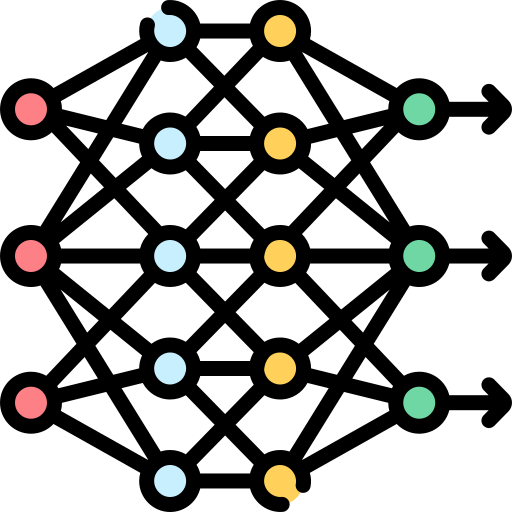
\includegraphics[width=0.75\textwidth]{figure/dlogo.png}
        \vfill
        {\Large Domenico Calò}\\
        \vspace{0.5cm}
        {\large A.A. 2024/2025}
        \vspace*{2cm}
    \end{center}
\end{titlepage}


\vspace*{\fill}

\begin{center}
    \textbf{Domenico Calò} \\
    \textit{Appunti di Deep Learning} \\
    Copyright~\textcopyright~2025
\end{center}

\vspace*{\fill}

\renewcommand{\baselinestretch}{1.2}\normalsize

\textsc{Colophon} \\
Questo lavoro è stato realizzato con \LaTeX{} su Mac utilizzando il pacchetto \textsf{ArsClassica}, uno stile ispirato a \textit{Gli elementi dello stile tipografico} di Robert Bringhurst. \\\\I nomi commerciali, i loghi, i marchi registrati menzionati negli appunti appartengono ai rispettivi proprietari, i pacchetti e le relative documentazioni ai rispettivi autori, le immagini presenti in questi appunti sono maggiormente prese dal web e appartengono ai rispettivi creatori.\\\\In caso di necessità dell'effetuare segnalazioni per eventuali, refusi aggiunte o correzioni, non esitate a contattarmi.
\vspace{1.5em}
\textsc{Contatti} \\
\faEnvelope[regular] \href{mailto:domenico.calo44@gmail.com}{\texttt{domenico.calo44@gmail.com}} · Contatta Domenico Calò
\newpage
\vspace*{\fill}

\begin{center}
    To ask the right question is harder than to answer it.\\
    — Georg Cantor
\end{center}

\vspace*{\fill}
\chapter*{Introduzione}

Questa dispensa nasce come supporto organico e approfondito al corso di \textbf{Deep Learning} tenuto dal \textbf{Prof. Vito Walter Anelli} nel secondo semestre del primo anno della \textbf{Laurea Magistrale} in \textbf{Ingegneria Informatica} presso il \textbf{Politecnico di Bari}. Il materiale raccolto e rielaborato in queste pagine ha l’obiettivo di fornire una guida completa e strutturata a tutti gli argomenti trattati durante il corso, seguendo passo dopo passo l’evoluzione delle tematiche affrontate a lezione, e integrando dove necessario approfondimenti teorici, esempi pratici e riferimenti alla letteratura scientifica, non cercando di elevare in maniera eccessiva il linguaggio di trattazione, in modo tale da risultare quanto più accessibile a tutti. Il Deep Learning è ad oggi una delle branche più attive e rivoluzionarie dell’Intelligenza Artificiale, con applicazioni che spaziano dalla visione artificiale alla comprensione del linguaggio naturale, dalla generazione di contenuti alla modellazione di fenomeni complessi. Per questo motivo, la presente dispensa non si limita a una trattazione superficiale, ma propone un percorso progressivo e dettagliato che accompagna il lettore dalla comprensione delle fondamenta teoriche fino alle architetture più avanzate e recenti della ricerca contemporanea.

Nel dettaglio, i capitoli che seguono coprono i seguenti macro-temi:
\begin{itemize}
    \item \textbf{Introduzione al Deep Learning}: origini, motivazioni, contesto storico e differenze rispetto al Machine Learning tradizionale;
    \item \textbf{Architetture di base}: reti neurali feedforward, backpropagation e capacità di rappresentazione;
    \item \textbf{Learning Representation}: apprendimento di rappresentazioni distribuite e significative;
    \item \textbf{Funzioni di attivazione e di costo}: ruolo, forme comuni e impatto sull’ottimizzazione;
    \item \textbf{Ottimizzatori}: algoritmi per la discesa del gradiente, tecniche avanzate e analisi della convergenza;
    \item \textbf{Normalization Layers}: normalizzazione dei dati all’interno delle reti per migliorare la stabilità dell’apprendimento;
    \item \textbf{Convolutional Neural Networks (CNN)}: architetture per il trattamento dei dati strutturati spazialmente (immagini);
    \item\textbf{Recurrent Neural Networks (RNN)}: modelli sequenziali e gestione della memoria nel tempo;
    \item\textbf{Generalizzazione e Overfitting}: tecniche e strategie per migliorare la capacità predittiva del modello su dati non visti;
    \item\textbf{Autoencoder}: modelli non supervisionati per la compressione e la generazione dei dati;
    \item\textbf{Generative Adversarial Networks (GAN)}: modelli generativi basati su apprendimento competitivo;
    \item\textbf{Transformer}: architettura basata sull’attenzione che ha rivoluzionato l’elaborazione sequenziale;
    \item\textbf{Modelli di Diffusione}: tecniche generative recenti, basate su processi stocastici inversi;
    \item\textbf{Graph Neural Networks (GNN) e Graph Convolutional Networks (GCN)}: reti neurali estese a dati strutturati come grafi;
\end{itemize}
Ogni capitolo è pensato per essere il più auto-contenuto possibile, pur mantenendo connessioni logiche con gli altri argomenti, in modo da offrire al lettore sia una visione modulare che sistemica della disciplina. Gli argomenti più complessi sono accompagnati da esempi, schemi esplicativi e, ove necessario, approfondimenti matematici volti a chiarire i meccanismi interni dei modelli. Questa dispensa vuole dunque porsi come un ponte tra teoria e pratica, utile non solo per la preparazione all’esame ma anche utile per stimolare la curiosità altrui, ad approfondire alcune tematiche trattate, come accade nel Capitolo~\ref{cap:14} e nel Capitolo~\ref{cap:15}.


\chapter*{Ringraziamenti}

Ringrazio in primis Lorenzo Pantieri, il quale inconsapevolmente, ha arricchito le mie personali conoscenze di \LaTeX, facendomi innamorare di questo mondo, semplicemente grazie ad alcuni suoi commenti presenti all'interno del forum del Gruppo Utilizzatori Italiani di \TeX{} e \LaTeX, ancora più in generale mi permetto di ringraziare inoltre tutti gli utenti e tutti i membri dello staff, che rendono quel forum una risorsa stupenda e meravigliosa di approfondimento, questo è l'internet che ci meritiamo e che personalmente gradisco e spero che non sparisca mai. Mi permetto di ringraziare il Prof. Vito Walter Anelli, il quale è stato in grado di raggiungermi con la sua passione per la materia del Deep Learning portandomi a scrivere questi appunti, senza di lui tutto ciò non sarebbe nemmeno esistito. Un ringraziamento speciale va ai miei colleghi che mi hanno accompagnato nel mio percorso universitario e che mi hanno arricchito personalmente, in particolare: Luca Crispino, Ivan Belvito, Antonio Favuzzi, Vincenzo Gentile, Monica Avella, Marzia Capuano, Elena De Michele, Fabrizio Ficarella e Luigi Racamato. Infine ci tengo a ringraziare tutti i futuri lettori di questi appunti, augurandoli un buono studio.
\tableofcontents
\listoffigures
\listoftables
\newpage

\chapter{Di cosa stiamo parlando}

In questo primo capitolo ci occuperemo di una semplice introduzione generale al Deep Learning, concentrandoci sul suo apetto a livello sociale ed effettuando anche dei riferimenti storici. Ovviamente tutto ciò che verrà trattato in questo capitolo, viene trattato con un livello di dettaglio, notevolmente ridotto, sorvolando anche su alcune cose, ma ciò può essere un ottimo punto di partenza, per poter approfondire diversi aspetti, sviluppando la curiosità del lettore. I modelli di Deep Learning sono oggi onnipresenti: li troviamo negli ospedali per la diagnosi automatica, in agricoltura per il monitoraggio delle colture, nella domotica per la gestione intelligente degli ambienti, negli assistenti virtuali, nei sistemi di rilevamento delle frodi, nella manutenzione predittiva degli impianti industriali e in molto altro.

\section{Applicazioni}

Le applicazioni del Deep Learning sono estremamente varie e in continua espansione, pertanto sarebbe pressocché impossibile elencarli tutti, di seguito elenchiamo solo alcuni dei possibili esempi di campi di applicazione:

\begin{itemize}
    \item Traduzioni automatiche (es. Google Translate, Google Lens, DeepL, Wordvice AI, ecc\dots);
    \item Sistemi di guida autonoma (es. Tesla Model S, EQS di Mercedes, BMW iX, e-tron GT di Audi, ecc\dots);
    \item Sistemi di raccomandazione (es. Netflix, Spotify, E-commerce, Outbrains, ecc\dots);
    \item Generazione automatica di testi, poesie, e immagini (es. DALL-E, Chat-GPT; Gemini, ecc\dots);
    \item Creazione di NPC (Non-Playable Characters) intelligenti nei videogiochi;
    \item Agenti intelligenti in grado di competere o superare gli esseri umani in diversi giochi.
\end{itemize}

\section{Evoluzione dei Modelli di AI}

Bisogna effettuare una precisazione prima di passare all'elenco di vari modelli, che hanno portato una rivoluzione nel mondo del Deep Learning. La storia dell'intelligenza artificiale, del Machine Learning e successivamente del Deep Learning, ha radici profonde, essa è fortemente radicata fin dai primi anni '50 grazie ad Alan Turing, il quale è stato un grande teoreta e svolse un importante ruolo durante la seconda guerra mondiale per quanto riguarda l'intercettazione dei messaggi dei tedesci, cifrati tramite algoritmi crittografici. A seguito di Turing, tutti questi argomenti hanno vissuto momenti di interessamento notevole da parte della comunità scientifica, e altri momenti di completo disinteresse, negli ultimi anni, in particolare a partire dagli anni '90, vi è stato un notevole incremento di interesse rispetto a queste tematiche, e pertanto ci limiteremo a raccontare alcuni eventi che si concentrano principalmente a partire da questo periodo.

\marginpar{\href{https://courses.cs.umbc.edu/471/papers/turing.pdf}{Turing, A. M. (1950). Computing machinery and intelligence. Mind, LIX(236), 433–460.~\cite{turing1950computing}}}
\subsubsection{1997 - Deep Blue}

Nel 1997, IBM sviluppa \textbf{Deep Blue}, il primo sistema di intelligenza artificiale in grado di sconfiggere il campione mondiale di scacchi in carica di quel momento, Garry Kasparov. Si trattava di un sistema basato su un’enorme potenza computazionale e un algoritmo di ricerca ottimizzato, allenato su numerose partite di scacchi, facendo sentire per la prima volta un umano, il quale aveva investito la sua intera vita per essere il campione mondiale di scacchi, impotente davanti a una macchina.

\subsubsection{2011 - Watson}

Nel 2011, sempre IBM, presenta \textbf{Watson}, un sistema in grado di rispondere a domande in linguaggio naturale. Watson vince il quiz televisivo \emph{Jeopardy!} contro i migliori concorrenti umani, dimostrando una capacità impressionante di comprensione del linguaggio e accesso alla conoscenza.

\subsubsection{2016 - AlphaGo}

Nel 2016, DeepMind (azienda di Google) sviluppa \textbf{AlphaGo}, il primo programma in grado di battere un campione mondiale di Go, Lee Sedol. A differenza di Deep Blue, AlphaGo invece utilizza delle tecniche più avanzate di deep learning e reinforcement learning, avendo un impatto ancor più straordinario, anche perché il gioco del Go, è sempre stato considerato un gioco più complesso degli scacchi.

\begin{figure}[htbp]
    \centering
    \begin{tcolorbox}[colframe=cyan!50!black, colback=cyan!10, boxrule=0.8mm, top=2mm, bottom=2mm, left=2mm, right=2mm]
        \begin{subfigure}[b]{0.45\textwidth}
            \centering
            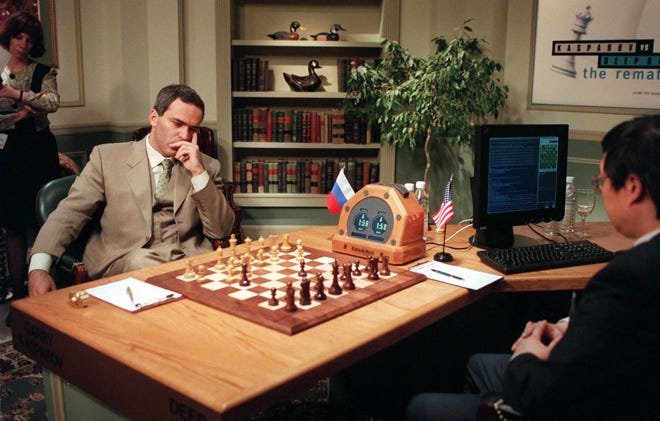
\includegraphics[width=\linewidth]{figure/GKDB.jpg}
            \caption{La celebre partita tra Kasparov e Deep Blue.}
            \label{fig:kasparovAndDeepBlue}
        \end{subfigure}
        \hspace{1cm}
        \begin{subfigure}[b]{0.45\textwidth}
            \centering
            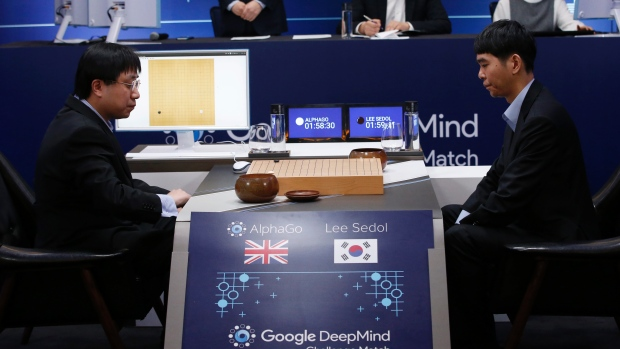
\includegraphics[width=\linewidth]{figure/AGLS.jpg}
            \caption{La storica sfida tra Lee Sedol e AlphaGo.}
            \label{fig:leeSedolAndAlphaGo}
        \end{subfigure}
    \end{tcolorbox}
    \caption{Sfide emblematiche tra esseri umani e intelligenze artificiali.}
    \label{fig:kasparovAndLeeSedol}
\end{figure}

\subsubsection{2017 - AlphaZero}

Nel 2017, DeepMind sviluppa \textbf{AlphaZero}, un sistema generalista capace di imparare a giocare a Go, scacchi e Shogi esclusivamente tramite autoapprendimento, senza l’ausilio di partite umane pregresse. Questo rappresenta un punto di svolta nell’addestramento tramite self-play.

\subsubsection{2017 - Agenti per StarCraft}

Blizzard, in collaborazione con DeepMind, inizia a sviluppare agenti intelligenti capaci di giocare a \emph{StarCraft II}, un gioco particolarmente complesso per via dell’alto numero di azioni e della parziale informazione, segnando questo agente come uno dei primi in assoluto a essere in grado di interagire con un videogioco.

\subsubsection{2016–2019 - OpenAI Five}

Tra il 2016 e il 2019, OpenAI sviluppa \textbf{OpenAI Five}, un agente capace di giocare a \emph{Dota 2}, vincendo contro team professionisti in una modalità 5 contro 5. Si tratta di una delle dimostrazioni più sofisticate di intelligenza artificiale collaborativa.

\subsubsection{2019 - AlphaStar}

Nel 2019, DeepMind introduce \textbf{AlphaStar}, che raggiunge prestazioni da livello campione mondiale in \emph{StarCraft II}, grazie a una combinazione di reinforcement learning, imitazione e tecniche avanzate di training multi-agente.

\subsubsection{2018–2020 - AlphaFold 2}

Tra il 2018 e il 2020, DeepMind sviluppa \textbf{AlphaFold 2}, un sistema rivoluzionario in grado di prevedere la struttura tridimensionale delle proteine con un'accuratezza senza precedenti, partendo dalla sola sequenza amminoacidica.

\subsubsection{2018–2020 - BERT}

Google introduce \textbf{BERT} (Bidirectional Encoder Representations from Transformers), un modello per la comprensione contestuale del linguaggio, che consente una rappresentazione semantica più profonda rispetto ai modelli precedenti.

\subsubsection{2021 - DALL·E}

Nel 2021, OpenAI presenta \textbf{DALL·E}, un modello generativo capace di produrre immagini realistiche a partire da descrizioni testuali.

\subsubsection{2022 - ChatGPT}

Nel 2022, OpenAI introduce \textbf{ChatGPT}, un \textbf{LLM} (Large Language Model) capace di generare risposte coerenti e plausibili, con un’interfaccia conversazionale estremamente naturale, pur con limiti di accuratezza.

\subsubsection{2023 - Bard}

Nel 2023, Google rilascia \textbf{Bard}, un LLM concorrente di ChatGPT. Tuttavia, a causa di alcune imprecisioni e problemi di affidabilità nelle risposte, viene rapidamente ritirato.

\subsubsection{2023 - Gemini}

Sempre nel 2023, Google lancia \textbf{Gemini}, un modello multimodale progettato per gestire contemporaneamente testo, immagini e audio, aprendo la strada a interazioni AI più complesse e versatili.

\begin{center}
    \begin{tikzpicture}[scale=0.75, every node/.style={transform shape, draw, rounded corners, align=center, font=\small, text width=2.5cm}, node distance=0.8cm]
        \node (1997) [fill=red!30] {1997\\Deep Blue};
        \node (2011) [fill=blue!30, below=of 1997] {2011\\Watson};
        \node (2016) [fill=green!30, right=of 2011] {2016\\AlphaGo};
        \node (2017) [fill=yellow!30, below=of 2016] {2017\\AlphaZero};
        \node (2019) [fill=purple!30, right=of 2017] {2019\\AlphaStar};
        \node (2020) [fill=orange!30, below=of 2019] {2020\\AlphaFold 2};
        \node (2021) [fill=cyan!30, right=of 2020] {2021\\DALL·E};
        \node (2022) [fill=pink!30, below=of 2021] {2022\\ChatGPT};
        \node (2023) [fill=gray!30, right=of 2022] {2023\\Bard/Gemini};
        
        \draw[->, thick] (1997) -- (2011);
        \draw[->, thick] (2011) -- (2016);
        \draw[->, thick] (2016) -- (2017);
        \draw[->, thick] (2017) -- (2019);
        \draw[->, thick] (2019) -- (2020);
        \draw[->, thick] (2020) -- (2021);
        \draw[->, thick] (2021) -- (2022);
        \draw[->, thick] (2022) -- (2023);
    \end{tikzpicture}
    
    \vspace{0.5em}
    \textbf{Figura 1:} Evoluzione cronologica dei principali modelli di Deep Learning dal 1997 al 2023.
\end{center}

\subsubsection{Conclusione}

Quelli analizzati finora rappresentano solo una minima parte dell'enorme ecosistema di modelli di Deep Learning sviluppati negli ultimi decenni. Sono stati scelti solo alcuni di essi legati, alla loro rilevanza nel corso del Prof. Anelli. L'esplosione e la diffusione di questi modelli sono dovute a ingenti investimenti specialmente da parte di aziende private ma anche da parte di enti governativi, rendendo l'Intelligenza Artificiale un settore strategico globale. Tutto ciò ci permette di comprendere a grandi linee qual è stata la progressione naturale e i maggiori focus su degli specifici task su cui ci si è soffermati negli ultimi anni da parte dell'AI, in modo da permetterci di capire soprattutto come siamo giunti agli attuali sviluppi.

\section{Aspetti Etici e Sicurezza}

L'espansione dell'intelligenza artificiale ha sollevato specialmente degli interrogativi etici, sociali e legali. Tra le principali preoccupazioni troviamo la sostituzione dell’essere umano in diversi settori lavorativi, la perdita di privacy, i rischi legati alla sicurezza e l’insufficiente trasparenza di molti sistemi. Il ruolo delle istituzioni pertanto, diventa centrale nell'effettuare una giusta regolamentazione, ma anche i ricercatori hanno la responsabilità di considerare le implicazioni etiche delle tecnologie che sviluppano, ovviamente è risaputo come effettuare dei controlli sulla sicurezza porta un dispendio di costi ulteriore e dei rallentamenti dal punto di vista commerciale, e proprio per questo molte aziende che si occupano di ciò sottovalutano questi aspetti concentrandosi principalmente su un fine commerciale.

\subsection{Banche dati esposte}

In diversi casi, database contenenti dei dati biometrici, come il riconoscimento facciale o tattile, sono stati archiviati senza aver adottato in precedenza delle adeguate misure di sicurezza, esponendo i dati sensibili degli utenti a rischi di uso improprio, questa cosa si è venuta a verificare molto spesso in dei contesti autoritari o militari, dunque dei contesti nei quali la perdita di informazioni di una tale sensibilità è notevolmente pericolosa.

\subsection{Bias}

L’intelligenza artificiale può riflettere e amplificare i bias presenti nei dati di addestramento. Un bias è un preconcetto, che una determinata persona può avere, a causa del contesto in cui si è cresicuti e alle cose a cui si è stati esposti, portandola a pensare in una determinata maniera, al di fuori dall'astrazione di una qualsivolgia forma di oggettività, infatti possono esistere delle persone le quali hanno delle ideologie politiche, idee religiose, sociali, culturali diverse, portando a un Bias rilevante nel momento in cui si cerca di giudicare un argomento in maniera quanto più oggettiva possibile. L'inteliggenza artificiale è fortemente condizionata dai Bias, presenti nei dataset sui quali viene allenata, alcuni esempi includono discriminazioni razziali nei modelli di giustizia predittiva o disparità di genere in modelli di selezione automatica del personale.

\subsection{Filter Bubble}
La \textit{filter bubble} (in italiano: bolla di filtraggio) è un concetto sviluppato da Eli Pariser nel suo libro \textit{The Filter Bubble: What the Internet Is Hiding from You (2011)}. Indica un ambiente informativo personalizzato in cui un individuo è esposto principalmente a contenuti che confermano le sue convinzioni preesistenti, mentre informazioni opposte o divergenti vengono filtrate o nascoste da algoritmi online. Una filter bubble si crea quando algoritmi (di Google, Facebook, YouTube, TikTok, ecc\dots) selezionano e mostrano contenuti in base ai tuoi interessi, click, like, cronologia di navigazione, e comportamenti passati, limitando così l’esposizione a idee differenti o contrastanti.

\subsection{Polarization Effect}

Una conseguenza della filter bubble, è sicuramente la polarizzazione, la quale scatena il polarization effect: gruppi omogenei finiscono per rafforzare le proprie opinioni in modo estremo, con conseguente aumento della divisione sociale, come visibile nei dibattiti online su temi sensibili. Questa cosa sicuramente non restituisce un'immagine reale della realtà poiché si vede tutto in maniera polarizzata, per l'appunto, dando pieno valore ai pareri estremi e non valutando tutte le possibili sfumature di grigio le quali possono essere presenti all'interno di un discorso.

\subsection{Adversarial Attacks}

Un \textit{adversarial attack} (in italiano: attacco avversario) è una tecnica utilizzata per ingannare un modello di machine learning, in particolare i modelli di deep learning, introducendo piccole perturbazioni appositamente progettate nei dati di input, tali da causare errori di classificazione o comportamenti indesiderati, senza che l’errore sia evidente a un osservatore umano. Un classico esempio è quello di immaginarsi un modello che classifica correttamente un’immagine come "papera". Se aggiungiamo una perturbazione invisibile all’occhio umano, il modello potrebbe classificare questa papera come "cavallo" con altissima confidenza e sicurezza, pur sembrando a noi ancora un papera (Figura~\ref{fig:adattack}).

\begin{figure}
    \centering
    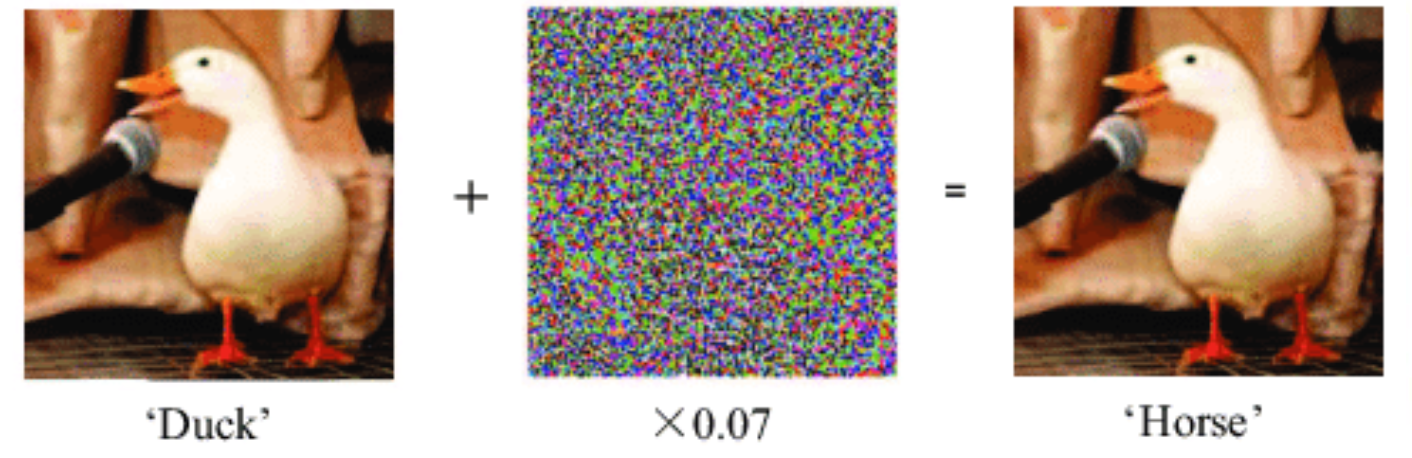
\includegraphics[width=0.75\textwidth]{figure/AdversarialAttack.png}
    \caption{Esempio di Adversarial Attack, in cui una papera viene classificata come cavallo a seguito dell'aggiunta di un rumore esterno.}
    \label{fig:adattack}
\end{figure}

\subsection{Data Poisoning}
Il \textit{data poisoning} è una forma di attacco contro i sistemi di machine learning in cui un attaccante manipola i dati di addestramento allo scopo di compromettere il comportamento del modello durante l’inferenza. Il data poisoning è come "avvelenare il cibo del cervello dell’IA": se il modello impara da dati falsificati o manipolati, finirà per imparare cose sbagliate. Questa tipologia di attacco risulta essere una vera e propria minaccia per la sicurezza e affidabilità dei modelli, soprattutto in contesti critici (sanità, difesa, veicoli autonomi). Questo è anche un ruolo molto critico, difficile da rilevare, specialmente nei modelli addestrati su dati pubblici o crowdsourced (es. GitHub, Kaggle, internet).


\subsection{Federated Learning}

Il \emph{federated learning} è un paradigma che consente l’addestramento distribuito del modello direttamente sui dispositivi degli utenti, migliorando la privacy e riducendo la necessità di centralizzare dati sensibili (Figura~\ref{fig:FedLearning}).

\begin{figure}
    \centering
    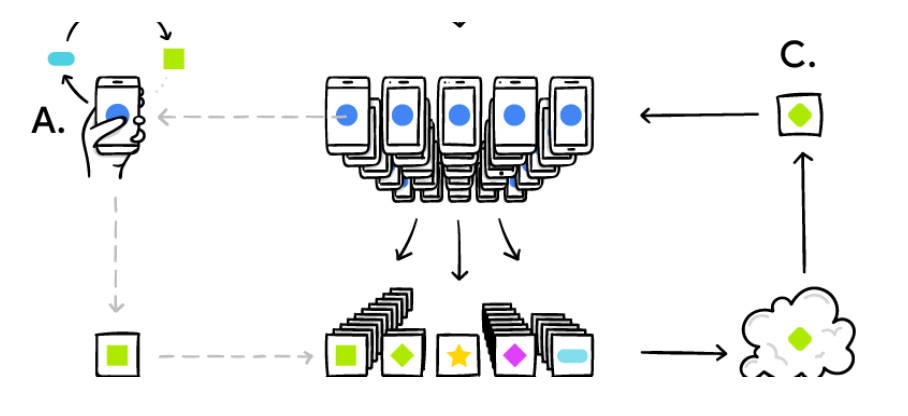
\includegraphics[width=0.85\textwidth]{figure/FederatedLearning.png}
    \caption{Architettura rappresentativa del Federated Learning.}
    \label{fig:FedLearning}
\end{figure}

\subsection{Sostenibilità e AI}

L’addestramento dei modelli di AI comporta un notevole consumo energetico. Ad esempio, GPT-3 ha richiesto risorse ingenti, contribuendo significativamente all’impatto ambientale. È quindi fondamentale sviluppare tecnologie più sostenibili, attraverso hardware efficiente e tecniche di training più leggere.

\subsection{AI Act}

L’\textbf{AI Act} dell’Unione Europea è una proposta legislativa che mira a classificare i sistemi di intelligenza artificiale secondo il livello di rischio. I sistemi ad alto rischio saranno soggetti a requisiti più stringenti, mentre quelli a basso rischio avranno meno restrizioni, promuovendo al contempo trasparenza e responsabilità.

\chapter{Introduzione al Deep Learning}

Ciò che bisogna consolidare prima di immergerci nello studio del Deep Learning è la differenza fra Machine Learning e Deep Learning. Per far questo bisogna analizzare quello che si fa con i programmi di Machine Learning, riferiamoci a uno specifico caso d'uso. Partiamo considerando il riconoscimento di un'immagine. Nel Machine Learning si parte dal creare un programma, il quale deve essere in grado, data un'immagine, di estrarre alcuni attributi per poi utilizzarli all'interno di un modello di ML e riconoscere immagini della stessa tipologia. Il passo ulteriore che viene effettuato nel Deep Learning è a monte, ossia durante la selezione degli attributi, quì noi costruiamo una gerarchia degli stessi, avendo la possibilità di stabilire attributi di basso, medio e alto livello. Questa selezione avviene con la combinazione di modelli di Machine Learning, creando nella sua complessità un meccanismo automatico più raffinato e profondo, da cui nasce il Deep Learning.

\begin{figure}
    \centering
    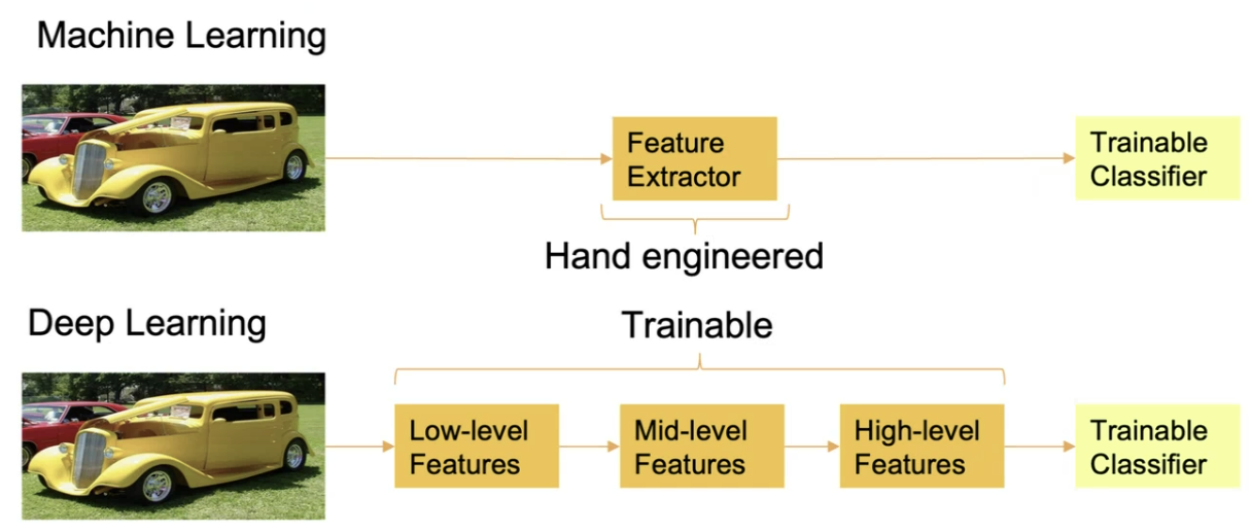
\includegraphics[width=0.75\linewidth]{figure/DeepMachineDiff.png}
    \caption{Schema rappresentativo della principale differenza fra un modello di Machine Learning e di Deep Learning}
    \label{fig:DLMLDiff}
\end{figure}

\section{Definizione}
Il Deep Learning dunque è una sotto-disciplina del Machine Learning la quale utilizza reti neurali profonde, ossia delle reti neurali con numerosi hidden-layer, per poter estrarre delle rappresentazioni gerarchiche dai dati. A differenza dei metodi tradizionali di Machine Learning, i quali richiedono l'ingegnerizzazione manuale delle caratteristiche, il Deep Learning è in grado di apprendere automaticamente rappresentazioni multi-livello, direttamente dai dati grezzi. Questo approccio, si è dimostrato particolarmente efficace in campi come la visione artificiale, il riconoscimento vocale e l'elaborazione del linguaggio naturale.

\section{Esempio: Il dataset MNIST}
MNIST è un dataset ampiamente utilizzato per il riconoscimento di cifre scritte a mano. Composto da 60.000 immagini di addestramento e 10.000 immagini di test, ognuna delle quali è una griglia $28\times28$ di pixel in scala di grigi. L'obiettivo di un modello di apprendimento automatico addestrato su MNIST, risulta essere quello di classificare correttamente ogni immagine in una delle 10 categorie (da 0 a 9). Questo dataset viene spesso utilizzato come benchmark, per poter valutare le prestazioni di nuovi algoritmi di apprendimento profondo.
\\
\begin{figure}[ht]
    \centering
    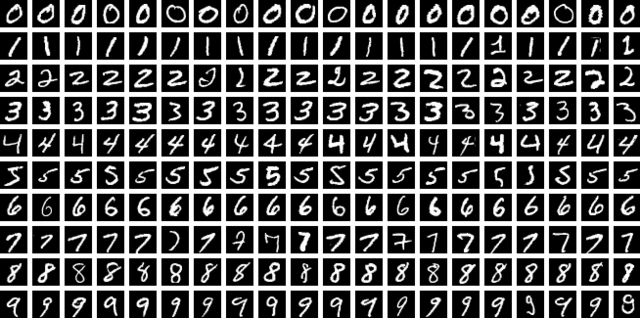
\includegraphics[width=0.75\textwidth]{figure/MNIST_dataset_example.png}
    \caption{Un estratto delle immagini presenti all'interno del dataset del MNIST.}
\end{figure}

\section{Grafi Computazionali}
Un Grafo computazionale rappresenta il flusso di operazioni effettuate tra variabili, viene utilizzato per modellare i calcoli svolti da una rete neurale. Ogni nodo del grafo rappresenta un'operazione matematica, mentre i bordi o archi, rappresentano i flussi di dati. Utilizzando questa struttura, possiamo visualizzare il flusso delle informazioni e il processo di apprendimento della rete. Ad esempio, in una rete neurale profonda, ogni livello applica una trasformazione, tramite l'utilizzo di una funzione di attivazione generando un output, il quale verrà poi propagato fino al livello finale, per ottenerne una previsione. Il modello utilizzato da noi, distingue nettamente i vari elementi tramite l'utilizzo di forme e colori, in modo da essere maggiormente intuitivo, avendo una differenza fra input, funzioni deterministiche e funzioni scalari (Figura~\ref{fig:parModel}).

\begin{figure}
    \centering
    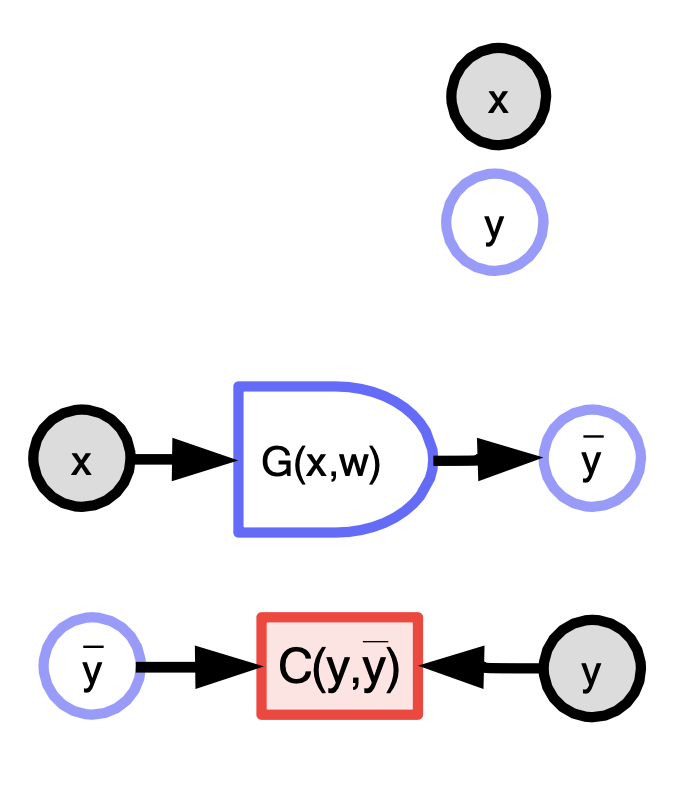
\includegraphics[width=0.40\linewidth]{figure/ParametriModel.png}
    \caption{Notazione dei nostri modelli, dall'alto verso il basso ci sono: Variabili, Funzione deterministica e Funzione scalare}
    \label{fig:parModel}
\end{figure}

\section{Funzione di costo}
Una \textbf{Funzione di Costo} è un'operazione riportabile tramite l'utilizzo dei nostri grafi computazionali (Figura~\ref{fig:costFunction}). Questa funzione misura l'errore pesente tra l'output fornito dal modello, dunque una predizione e l'output desiderato, essa, risulta essere fondamentale per il processo di apprendimento. Il modello, cerca di minimizzare questa funzione di costo, in inglese Loss Function (per questo si parla spesso di perdita), aggiustando i pesi della rete di volta in volta attraverso un algoritmo di ottimizzazione. Una delle funzioni di costo più comuni è la Mean Squared Error (MSE), definita come:
\begin{equation}
    C(y, \hat{y}) = \frac{1}{n} \sum_{i=1}^{n} (y_i - \hat{y}_i)^2
\end{equation}
Dove $y_i$ rappresenta il valore reale e $\hat{y}_i$ l'output predetto dal modello per il campione $i$-esimo. Minore è il valore della funzione di costo, migliore sarà la capacità del modello di effettuare previsioni accurate.

\begin{figure}
    \centering
    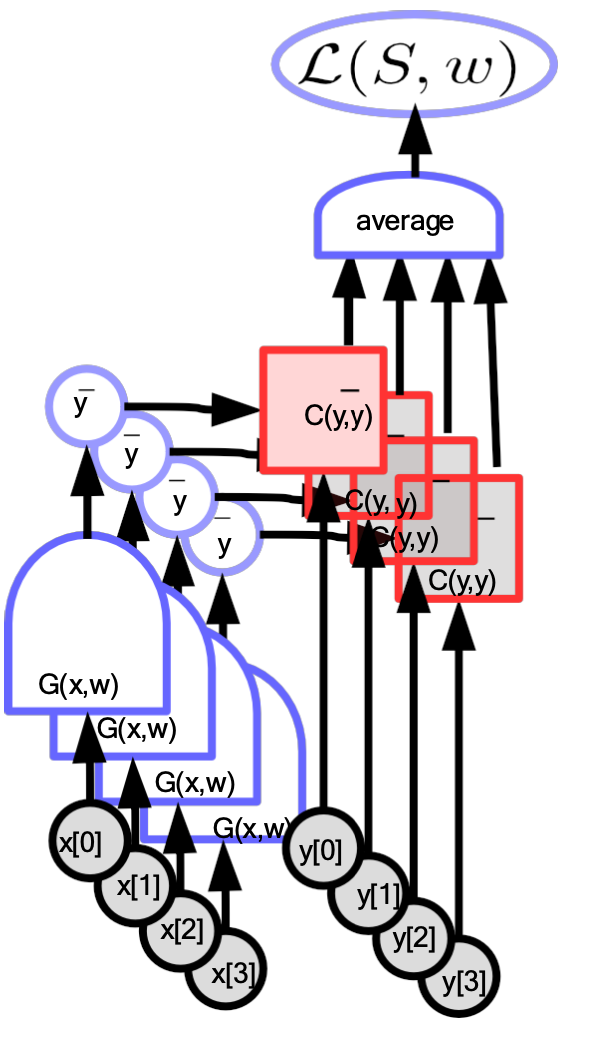
\includegraphics[width=0.30\linewidth]{figure/CostFunction.png}
    \caption{Rappresentazione tramite l'utilizzo di un grafico computazionale della funzione di costo, utilizzando la MSE}
    \label{fig:costFunction}
\end{figure}

\section{Reti Neurali}
Una Rete Neurale, tramite i nostri grafi computazionali, risulta essere una pila di blocchi funzionali lineari e non lineari. Le loro entità fondamentali prendono il nome di neuroni(Figura~\ref{fig:neuralNet}). Ogni \textbf{neurone} calcola una somma pesata degli input ricevuti e applica una funzione di attivazione per introdurre non linearità nel modello. Questa architettura, permette alla rete di apprendere rappresentazioni complesse dei dati. Un singolo neurone in una rete neurale può essere rappresentato come segue:
\begin{equation}
    z = \sum_{i=1}^{n} w_i x_i + b
\end{equation}
Dove $w_i$ sono i pesi associati agli input $x_i$, e relativi al bias $b$ (un peso costante che va sommato agli altri pesi). Successivamente, viene applicata una funzione di attivazione $\sigma(z)$ in modo tale da ottenere un output finale:
\begin{equation}
    y = \sigma(z)
\end{equation}

Le reti neurali, sono strutture complesse composte da tanti neuroni, i quali possono essere completamente collegati fra loro, generando le \textit{Fully-Connected Neural Network}, oppure collegate parzialemente creandone di diversa tipologia, i neuroni vengono concatenati formando diversi strati, dando la possibilità di formare delle archittetture profonde, composte da diversi strati.

\begin{figure}[ht]
    \centering
    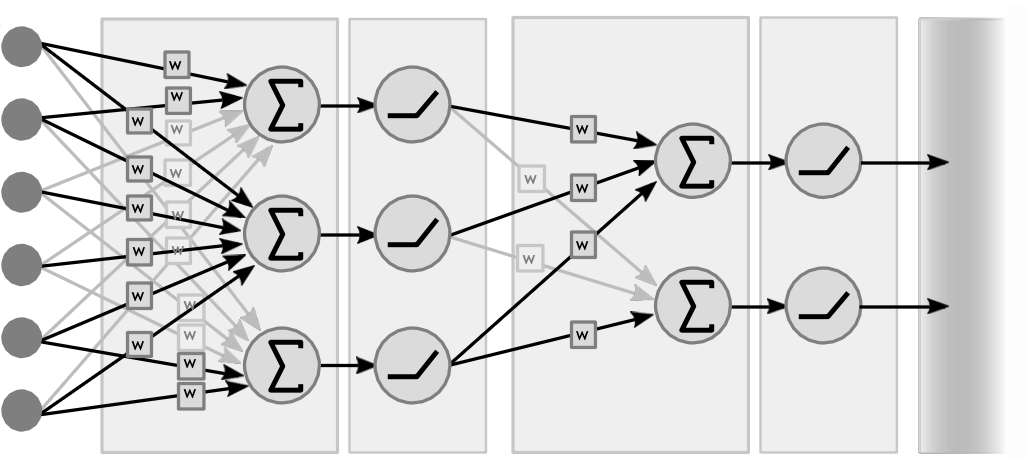
\includegraphics[width=0.85\textwidth]{figure/NeuralNet.png}
    \caption{Figura rappresentativa di un esempio di rete neurale con diversi strati nella sua architettura.}
    \label{fig:neuralNet}
\end{figure}

\section{Backpropagation}
La \textbf{Backpropagation} (retropropagazione), è uno degli algoritmi principali quando si parla di reti neurali, poiché permette di allenare la rete, basandosi sulla \textbf{discesa del gradiente}.
\begin{Definizione}
    La discesa del gradiente è un algoritmo di ottimizzazione che trova il valore minimo di una funzione, spostandosi iterativamente nella direzione opposta al suo gradiente. 
\end{Definizione}
L'idea della Backpropagation, è quella di propagare all'indietro l'errore generato dalla predizione e dal valore effettivo, in modo da aggiornare i pesi della rete, in modo che venga ridotto l'errore complessivo (la loss function). Il processo di Backpropagation consente di calcolare i gradienti dell'errore, rispetto ai pesi della rete e poter propagare questi gradienti attraverso la rete all'indietro, in modo tale da aggiornare i pesi e ottenere dei risultati sempre più accurati di volta in volta fintantoché non si raggiunge a una convergenza dei valori dei pesi.

\subsection{Calcolo dei Gradienti}
Il cuore della Backpropagation risiede nel calcolo dei gradienti della loss function rispetto ai pesi, utilizzando la \textbf{regola della catena}.
\begin{Definizione}
    La regola della catena afferma che se $f(x)$ e $g(x)$ sono funzioni derivabili, allora la derivata della funzione composta $h(x) = f(g(x))$ è:
    \[
    \frac{\partial h}{\partial x} = \frac{\partial f}{\partial g} \cdot \frac{\partial g}{\partial x}
    \]
\end{Definizione}
\marginpar{\href{https://cannydatascience.medium.com/backpropagation-come-apprende-una-rete-neurale-91c0c900fbc}{Approfondimento sulla Backpropagation}}
L'algoritmo di Backpropagation calcola i gradienti da ogni layer e li propaga all'indietro, aggiornando i pesi della rete. Il gradiente indica la direzione nella quale i pesi devono essere aggiornati per ridurre l'errore complessivo. La formula generale per la derivata della funzione di costo rispetto ai pesi è la seguente:
\begin{equation}
    \frac{\partial C}{\partial W} = \frac{\partial C}{\partial y} \cdot \frac{\partial y}{\partial W}
\end{equation}
Dove $C$ rappresenta la funzione di costo, $y$ l'output del modello e $W$ il peso da aggiornare. Questo processo viene ripetuto per ogni livello della rete, fino all'ottimizzazione del valore dei pesi. Questa procedura può essere facilmente sintetizzata in un grafo computazionale (Figura~\ref{fig:backPropGraph}). Nell'algoritmo della backpropagation è possibile applicare qualunque grafo che sia diretto e aciclico. Nel caso in cui il grafo presentasse dei loop, sarà necessario scioglierli.

\begin{figure}
    \centering
    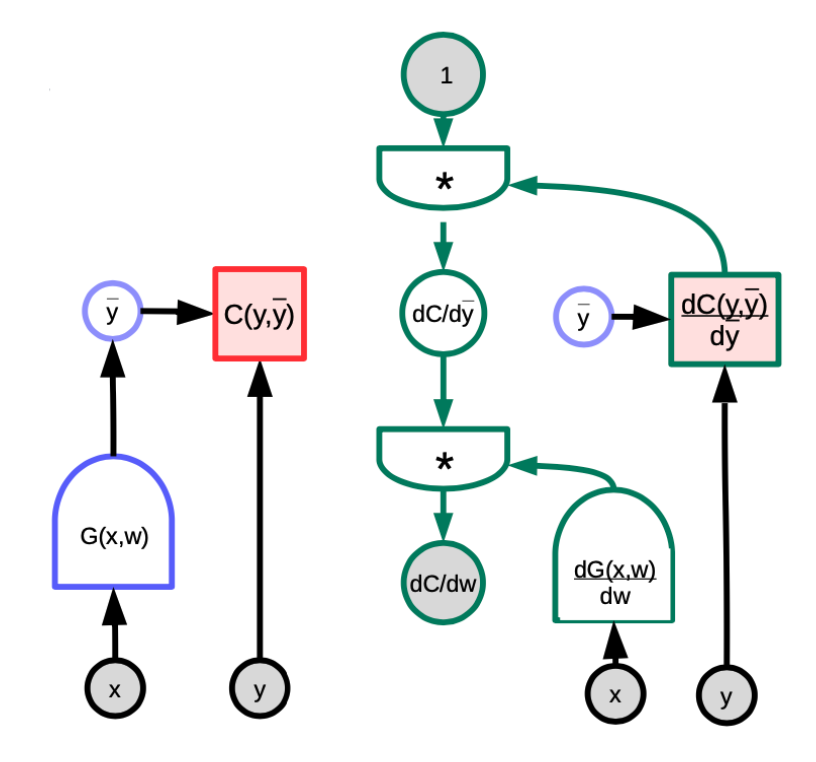
\includegraphics[width=0.5\linewidth]{figure/BackPropGraph.png}
    \caption{Grafo computazionale della Backpropagation, che si integra con quello già precedentemente visto della funzione di costo in modo tale da raffinare gli esiti finali correggendosi dinamicamente}
    \label{fig:backPropGraph}
\end{figure}

\section{Problemi della Backpropagation}
La Backpropagation soffre di due principali problemi ossia quello del \textit{gradiente che scompare} e quello che \textit{esplode}. Questi due problemi si verificano quando il gradiente della funzione di costo, rispetto ai pesi, risulta essere molto piccolo o molto grande nei livelli più profondi della rete.

\begin{itemize}
    \item \textbf{Gradiente che scompare:} nelle reti molto profonde, i gradienti calcolati per i livelli iniziali diventano sempre più piccoli man mano che vengono propagati all'indietro. Questo provoca degli aggiornamenti minimi dei pesi nei primi livelli, rallentando drasticamente l'addestramento o impedendo alla rete di apprendere;
    \item \textbf{Gradiente che esplode:} al contrario, se i gradienti aumentano esponenzialmente durante la propagazione all'indietro, i pesi della rete possono diventare estremamente grandi, portando a instabilità nell'addestramento e rendendone difficile la convergenza.
\end{itemize}

Con il passare degli anni il Machine Learning evolvendosi e specializzandosi nel Deep Learning, portando allo sviluppo di diverse soluzioni per queste problematiche:

\begin{enumerate}
    \item \textbf{Funzioni di attivazione avanzate:} L'utilizzo di altre funzioni come \textbf{ReLU} (Rectified Linear Unit) la quale ha ridotto il problema del gradiente che scompare rispetto alla funzione $\operatorname{sigmoid}$ e $\operatorname{tanh}$. Varianti come $\operatorname{Leaky\,ReLU}$ e $\operatorname{Parametric\,ReLU}$ migliorano ulteriormente l'apprendimento;
    \item \textbf{Inizializzazione dei pesi:} Metodi di inizializzazione dei pesi come \textbf{Xavier} per l'assegnamento dei pesi stabilizzano i gradienti all'inizio dell'addestramento;
    \item \textbf{Batch Normalization:} Tecnica la quale permette di normalizzare le attivazioni intermedie riducendo la varianza dei gradienti durante la propagazione.
\end{enumerate}

L'introduzione infatti di queste e altre tecniche, hanno permesso al Deep Learning di diventare un campo di studio sempre più interessante, divenendo anche più efficace come tecnica rispetto all'utilizzo di metodi tradizionali postulati dal Machine Learning.

\section{Implementazione con PyTorch}
Per effettuare una parallelizzazione della teoria, con l'aspetto implementativo del Deep Learning, quì mostriamo come implementare una rete neurale utilizzando \textbf{PyTorch}, per far ciò possiamo utilizzare la classe \texttt{nn.Module} in modo tale da definire la nostra architettura. Di seguito un esempio di una semplice rete con due livelli nascosti:
\\
\begin{python}[frame=trBL]
    import torch
    from torch import nn

    class MyNet(nn.Module):
        def __init__(self, input_dim, hidden_dim, output_dim):
            super().__init__()
            self.fc1 = nn.Linear(input_dim, hidden_dim)
            self.fc2 = nn.Linear(hidden_dim, output_dim)
    
        def forward(self, x):
            x = torch.relu(self.fc1(x))
            x = self.fc2(x)
            return x
    model = MyNet(784, 128, 10)
\end{python}
\vspace{0.5em}
La rete in questo codice prende in input delle immagini di 28x28 pixel (convertite in vettori di 784 elementi), le elabora utilizzando un livello nascosto con 128 neuroni e produce infine un output di 10 neuroni corrispondenti alle 10 classi del dataset MNIST.
\chapter{Architetture di Base}

Quando si parla di Deep Learning, si usano spesso delle strutture grafiche, aggiungendo dei livelli di astrazione, per poter semplificare la comprensione delle architetture complesse, queste strutture prendono il nome di \textbf{Grafi Computazionali}. La rappresentazione grafica di alcuni dei modelli più complessi, permette di comprendere al meglio come vengono implementate alcune nuove tecniche. Adesso vedremo, semplici implementazioni, per dare un'idea di utilizzo, e lasciare a chi legge, la possibilità di adottarle nei propri progetti.

\section{Moduli moltiplicativi}
Iniziamo da delle architetture semplici: i moduli moltiplicativi. Creiamo immediatamente un collegamento con questi moduli, sfruttando un esempio pratico. Nel processo di backpropagation essi vengono utilizzati, poiché si può effettuare tale processo, rispetto agli input, o rispetto ai pesi. La differenza fra operare rispetto agli uno o gli altri si trova nell'impossibilità di imparare direttamente i pesi, come avviene per gli input. In molti hanno pensato cosa succederebbe nel caso in cui i pesi fossero gli output di un'altra Rete Neurale, questa possibilità viene sfruttata tramite i moduli moltiplicativi.

\begin{equation}
    s_i = \sum_{j}w_{ij}x_{j}\,:\, w_{ij}=\sum_ku_{ijk}z_k \Rightarrow s_i=\sum_{jk}u_{ijk}z_kx_j
    \label{eq:weightAsInput}
\end{equation}

Come vediamo nella formula di cui sopra, possiamo notare come, essa sia una sostituzione semplice, ottenendo comunque un risultato desiderato, senza modificare il senso dell'operazione. Questa semplice sostituzione, è stata adottata in molti contesti di Deep Learning.
\begin{figure}[htbp]
    \centering
    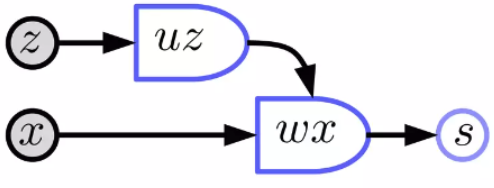
\includegraphics[width=0.4\linewidth]{figure/WeightAsInput.png}
    \caption{Grafo computazionale corrispettivo all'equazione~\ref{eq:weightAsInput}}
    \label{fig:wai}
\end{figure}

Se avessimo una Rete Neurale che si occupa del controllo dei pesi, saremmo in grado di crearne una nuova con una semplice variazione di essi, potendo persino ampliarne la portata riuscendo a controllarne molte reti con una a supervisionare. Questo non è un lavoro semplice, dovremmo effettuare delle limitazioni per non incorrere in problematiche di esplosione della rete stessa. Dunque la rete neurale al di sopra delle altre, funziona come un "controllore", pesando di più una sottorete piuttosto che un'altra (Figura~\ref{eq:attentionMod}). Questo meccanismo si implementa adoperando la funzione \textbf{SoftMax}, che tratteremo più avanti, essa ci permette di calcolare nuovi pesi ed effettuare un'attivazione. Questa architettura prende il nome di \textbf{Modulo dell'attenzione}, dando più o meno importanza in base all'input ricevuto alle singole reti neurali.

\begin{equation}
    s_i = \sum_jw_jx_{ij} \,:\,w_j=\frac{e^{z_{j}}}{\sum_ke^{z_k}}
    \label{eq:attentionMod}
\end{equation}

\begin{figure}[htbp]
    \centering
    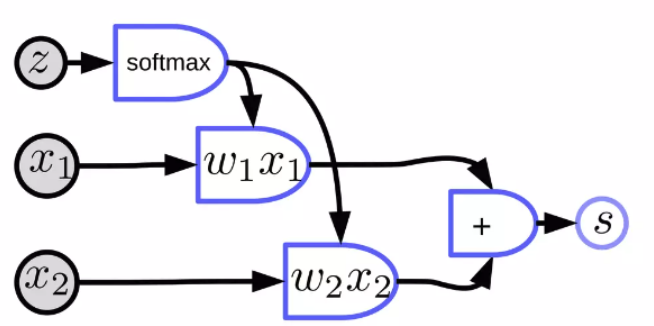
\includegraphics[width=0.4\linewidth]{figure/AttentionModule.png}
    \caption{Grafo computazionale rappresentante il Modulo dell'attenzione, in cui ci sono più reti, controllate da una singola, la quale da più o meno importanza alle sottoreti in base all'input ricevuto.}
    \label{fig:AttentionMod}
\end{figure}

\subsubsection{Mixture of Experts}
L'idea che stiamo analizzando, inserendo più reti neurali in un'unica architettura, prende il nome di \textbf{Mixture of Experts}, partendo da una semplice rete neurale con $x_1$ e $x_2$ come ingressi, la estendiamo rendendola un'\textit{esperta}, creando una rete con all'interno milioni di parametri. Il modello Mixture of Experts è una rete neurale, la quale controlla diversi task, spezzati nelle singole sottoreti, selezionando su quale fare affidamento a seconda della necessità (Figura~\ref{fig:mixExp}). I modelli di linguaggio, utilizzano questa strategia, prendono in considerazione una combinazione di reti specializzate in diverse attività (es. Traduzione, riassunto, calcoli, ecc\dots). 

\begin{figure}[htbp]
    \centering
    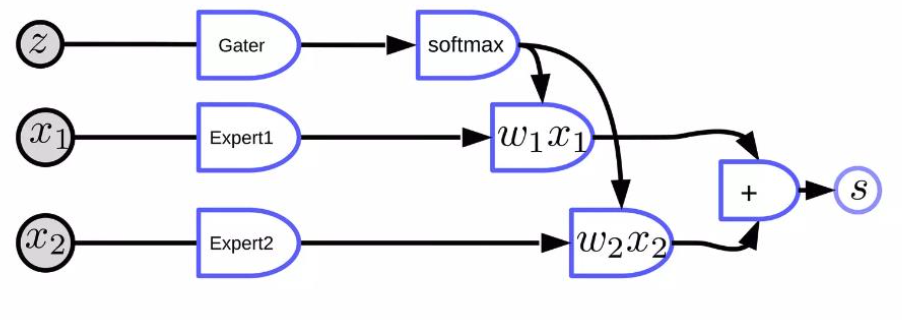
\includegraphics[width=0.5\linewidth]{figure/MixtureOfExpert.png}
    \caption{Grafo computazionale, del modello Mixture of Experts, vari modelli specializzati in compiti specifici, attivati o disattivati da un'altra rete neurale tramite l'utilizzo della funzione softmax.}
    \label{fig:mixExp}
\end{figure}

\subsubsection{Parameter Transoformation}

Un modo generale per concettualizzare architetture come la Mixture of Experts è attraverso l'idea di \textbf{Parameter Transformation}. Invece di considerare i parametri di un modello, come i pesi $W$, dei valori statici appresi una sola volta, li concepiamo come l'output dinamico di un altro modulo. In pratica, la rete impara a generare o selezionare i parametri più adatti in base al contesto fornito dall'input. L'architettura Mixture of Experts (MoE) può essere vista come un caso specifico di questo principio. In una MoE, la rete generale non crea nuovi pesi, ma seleziona quale set di parametri (quello di un "esperto") utilizzare. Differentemente la Parameter Transformation è un'operazione di selezione dinamica. Una delle applicazioni più diffuse di questo concetto è la \textit{Weight Sharing}. Questa tecnica consiste nell'utilizzare lo stesso modulo parametrico, definito da un set di pesi $w$, applicandolo ripetutamente in diverse parti di un modello o per elaborare porzioni differenti dell'input (Figura~\ref{fig:wshar}).

\begin{figure}[htbp]
    \centering
    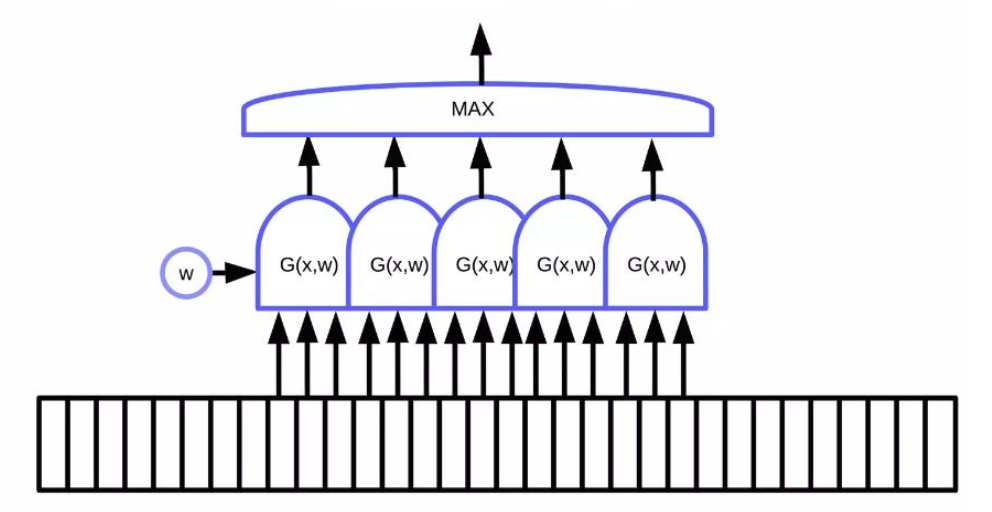
\includegraphics[width=0.65\linewidth]{figure/WeightShar.png}
    \caption{Esempio di grafo computazionale che implementa la Weight Sharing. Un unico set di parametri, il kernel $w$, riutilizzato ripetutamente dalla funzione $G$ su diverse sezioni dell'input.}
    \label{fig:wshar}
\end{figure}

Quindi si ha un modulo generatore di pesi, iniettato in diversi punti della rete principale permettendo di avere due vantaggi principali:

\begin{itemize}
    \item \textbf{Efficienza:} Invece di dover apprendere e memorizzare un set di pesi indipendente per ogni operazione, si apprende un unico e più compatto modulo che sa come generarli. Riduce drasticamente il numero totale di parametri del modello, rendendolo più leggero ed efficiente;
    \item \textbf{Generalizzazione:} Durante l'addestramento, il processo di backpropagation diventa particolarmente efficace. Se lo stesso modulo di pesi condivisi viene utilizzato in $N$ contesti diversi, esso riceverà i gradienti di errore da tutte e $N$ le funzioni di costo parziali. Questo "costringe" il modulo ad apprendere parametri che non siano specifici per un singolo compito, ma che siano abbastanza robusti da funzionare bene in tutte le situazioni. Porta a un risultato con una migliore capacità di generalizzazione.
\end{itemize}

\chapter{Learning Rappresentation}
\section{Introduzione}
Uno degli obiettivi fondamentali del Deep Learning è imparare rappresentazioni significative a partire da dei dati grezzi. Un buon modello di Deep Learning non si limita a classificare gli input, ma è in grado di riuscire a estrarre delle caratteristiche gerarchiche le quali semplificano notevolmente i compiti di analisi e previsione.

\section{Classificatori Lineari e i loro Limiti}
I classificatori lineari, i quali solitamente ci siamo trovati durante il corso di Machine Learning a interfacciarci, suddividono lo spazio degli input in due regioni separate da un iperpiano. Tuttavia, questa soluzione risulta essere molto limitata:
\begin{itemize}
    \item Non è in grado di gestire problemi con dati non linearmente separabili;
    \item La probabilità che una distribuzione casuale di punti $P$ sia separabile linearmente diminuisce all'aumentare della dimensionalità $N$ nel momento in cui $P \ge N$ (Teorema di Cover, 1966).
\end{itemize}

Per forza di cose nel caso in cui andassimo ad aumentare la dimensione di $N$ per cercare di arginare il problema, a causa del teorema di Cover dobbiamo fare anche attenzione anche alla \textit{Curse of Dimensionality}, la quale è anch'essa campo di studio.

\begin{figure}[!ht]
    \centering
    \begin{subfigure}[b]{0.45\textwidth}
        \centering
        \begin{tikzpicture}[scale=0.75]
            \draw[->, thick] (-1,0) -- (5,0) node[anchor=north] {\textbf{x1}};
            \draw[->, thick] (0,-1) -- (0,5) node[anchor=east] {\textbf{x2}};
            \node[below] at (2,0) {\textbf{-b/w1}};
            \draw[thick, dashed] (0.5,0) -- (4.5,4);
            \foreach \x/\y in {
                2/3.5, 1.2/3.8, 3.5/4, 2.8/4.2, 4/3.7,
                3.8/3.3, 3.2/4.1, 2.2/3.4, 3/3.8, 1.7/3.2
            } {
                \fill[blue] (\x,\y) circle (3pt);
            }
            \foreach \x/\y in {
                1/0.5, 2/1.5, 1.8/0.8, 3/1.2, 4/0.7,
                2.5/1.3, 3.5/0.9, 1.5/0.5, 3.2/1.7, 2.2/0.6
            } {
                \fill[red] (\x,\y) circle (3pt);
            }
        \end{tikzpicture}
        \caption{Dati linearmente separabili}
    \end{subfigure}
    \hfill
    \begin{subfigure}[b]{0.45\textwidth}
        \centering
        \begin{tikzpicture}[scale=0.75]
            \draw[->, thick] (-1,0) -- (5,0) node[anchor=north] {\textbf{x1}};
            \draw[->, thick] (0,-1) -- (0,5) node[anchor=east] {\textbf{x2}};
            \foreach \x/\y in {
                2/2, 2.2/2.2, 1.8/1.8, 2.1/1.9, 1.9/2.1,
                2/1.7, 2.3/2, 1.7/2.3, 2.1/2.4, 1.6/1.9
            } {
                \fill[blue] (\x,\y) circle (3pt);
            }
            \foreach \x/\y in {
                1/1, 3/3, 3.5/2.5, 2.5/3.5, 1.2/3.3,
                3.7/1.5, 0.8/2, 3.3/3.3, 2.8/0.8, 0.5/1.5
            } {
                \fill[red] (\x,\y) circle (3pt);
            }
            \fill[blue] (4.1,4.5) circle (3pt);
            \node[right] at (4.2,4.5) {\textbf{Classe 1}};
            \fill[red] (4.1,4) circle (3pt);
            \node[right] at (4.2,4) {\textbf{Classe 2}};
        \end{tikzpicture}
        \caption{Dati non linearmente separabili}
    \end{subfigure}

    \caption{Confronto tra un dataset linearmente separabile (a sinistra) e uno non linearmente separabile (a destra).}
    \label{fig:linear-vs-non-linear}
\end{figure}

\subsection{Soluzione: Rappresentazioni (Features)}
Per superare i limiti dei classificatori lineari, ci sono varie metodologie, una di queste è quella approfondita attraverso l'esempio della funzione \textbf{XOR}, visto nel corso di Machine Learning, dove per definizione la funzione XOR genera dei dati che non sono linearmente separabili, ma attraverso la combinazione di modelli più semplici, i quali ci permettono di attura la separabilità lineare, riusciamo a ottenere la funzione complessiva attraverso una rete neurale. Di seguito alcune metodologie per far fronte ai limiti dei classificatori lineari:
\begin{itemize}
    \item Estrarre caratteristiche rilevanti dall'input grezzo;
    \item Trasformare i dati in una rappresentazione in cui la separabilità lineare sia più semplice;
    \item Usare estrattori di caratteristiche non lineari, come reti neurali profonde.
\end{itemize}

\section{Metodi di Estrazione}
Alcuni metodi per estrarre caratteristiche utili includono:
\begin{itemize}
    \item \textbf{Tiling dello spazio}: suddivisione dello spazio in regioni più piccole.
    \item \textbf{Proiezioni casuali}: trasformazioni casuali per aumentare la dimensione dello spazio.
    \item \textbf{Classificatori polinomiali}: utilizzo di combinazioni di variabili di input per migliorare la separabilità.
    \item \textbf{Macchine a kernel}: mappatura non lineare dei dati in uno spazio a più alta dimensionalità.
\end{itemize}

Generalmente l'idea alla base di tutte queste possibilità è quella di poter espandere le dimensioni della nostra rappresentazione, per far sì che i nostri dati risultino essere facilmente lineramente separabili.

\begin{Osservazione}
    Ci potremmo chiedere del perché dovremmo usare soltanto le features in maniera lineare. La risposte è che diventa più semplice nella pratica, poiché nel momento in cui vado a considerare delle features che non lo sono, tutto risulterà più complesso a livello di costo computazionale.
\end{Osservazione}

\section{Reti Neurali Poco Profonde}
Per poter far fronte a quesat problemati, si possono utilizzare le strategie quì di seguito elencate:

\begin{itemize}
    \item Le macchine a vettori di supporto (SVM) e i metodi a kernel utilizzano uno strato con funzioni di base non lineari, seguito da uno strato lineare;
    \item Utilizzare delle reti neurali con due strati diventando degli approssimatori universali~\ref{th:Cybenko_1989}, tuttavia richiedono un numero elevato di neuroni per rappresentare funzioni complesse.
\end{itemize}

\begin{Teorema}
    Una rete con 2 strati (con 1 strato nascosto), è un approssimatore universale, può cioè approssimare in modo arbitrariamente preciso ogni funzione continua $g(u_1,u_2,\dots,u_d)$ (pur di prendere un numero sufficiente di neuroni).
    \label{th:Cybenko_1989}
\end{Teorema}

A fronte di questo teorema potremmo chiederci del perché con il Deep Learning, ci dobbiamo spingere a utilizzare delle reti neurali più profonde, visto che ogni funzione continua sia possibile rappresentarla anche con semplicemente un singolo layer nascosto.

\subsubsection{Perché le Architetture Profonde?}
La risposta viene trovata facilmente, poiché una rete neurale profonda è in grado di rappresentare funzioni complesse in modo più efficiente rispetto a una rete poco profonda, ma soprattuto, nel momento in cui passiamo a una rete neurale più profonda avremo un risultato in meno tempo, quindi abbiamo rinunciato a dello spazio per risparmiare del tempo. Inoltre esse hanno:
\begin{itemize}
    \item Maggiore capacità di modellare strutture gerarchiche nei dati  (es. riconoscimento visivo, riconosco una figura a seconda di sue diverse caratteristiche, ognuna analizzata in un layer);
    \item Possibilità di apprendere trasformazioni sempre più astratte dei nostri dati.
\end{itemize}

\section{Ipotesi del Manifold}
Un concetto molto importante del Deep Learning è l'ipotesi del \textbf{Manifold}, se volessimo riconoscere la faccia di una persona prendendo in analisi quella nella Figura~\ref{fig:manifold}, noi possiamo notare che in ognuna delle sottofigure vi è la stessa persona, è corretto interrogarsi sul perché noi umani, riusciamo a dire ciò. Molto semplicemente ci sono delle caratteristiche che noi riusciamo a riconoscere che appartengono alla stessa persona. Il nostro cervello, e più in generale, la nostra realtà si trova in uno spazio dimensionale che non è della stessa grandezza della figura che possiamo creare.

\begin{figure}[h]
    \centering
    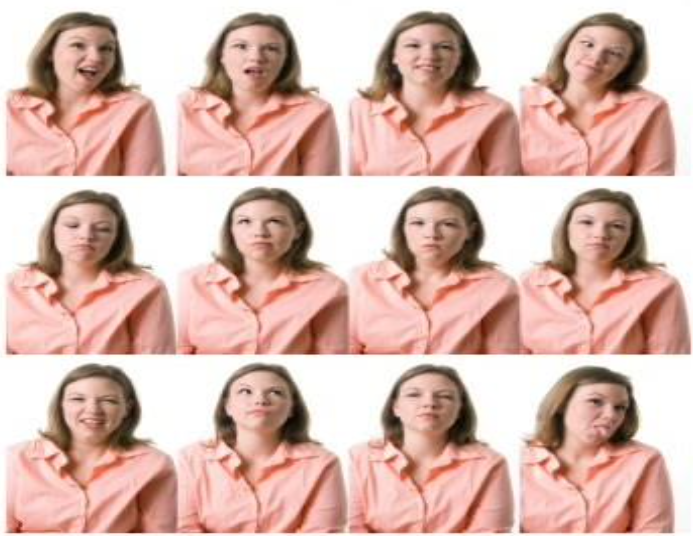
\includegraphics[width=0.45\textwidth]{figure/Manifold.png}
    \caption{Esempio dell'ipotesi del manifold.}
    \label{fig:manifold}
\end{figure}

\marginpar{L'argomento della Data Manifold, viene trattato di più in: \href{https://ieeexplore.ieee.org/stamp/stamp.jsp?tp=&arnumber=1640964}{Hadsell et al. CVPR 2006~\cite{hadsell2006dimensionality}}}

È stato dimostrato come noi umani, siamo in grado di riconoscere una faccia di una persona rappresentando meno di 56 variabili, mentre differentemente nel momento in cui usiamo un'immagine composta da $1000$x$1000$ pixel avrò $1\,000\,000$ di dimensioni per il nostro calcolatore. Questa è la così detta ipotesi del Manifold, ossia che la realtà vive in una dimensione molto minore rispetto alla dimensione che utiliziamo per rappresentarla. 

\subsubsection{Correlazione con cio che stiamo facendo}
Se avessimo un estrattore ideale, potremmo essere in grado di prendere questa immagine da un milione di dimensioni, e semplicemente estrarre queste 56 features, in modo tale da essere in grado di riconoscere l'immagine. Pertanto noteremo come muovendoci su un piano cartesiano, spostandoci lungo una singola dimensione cambieremo solo ed esclusivamente una singola features (Figura~\ref{fig:cartesianFig}).

\begin{figure}
    \centering
    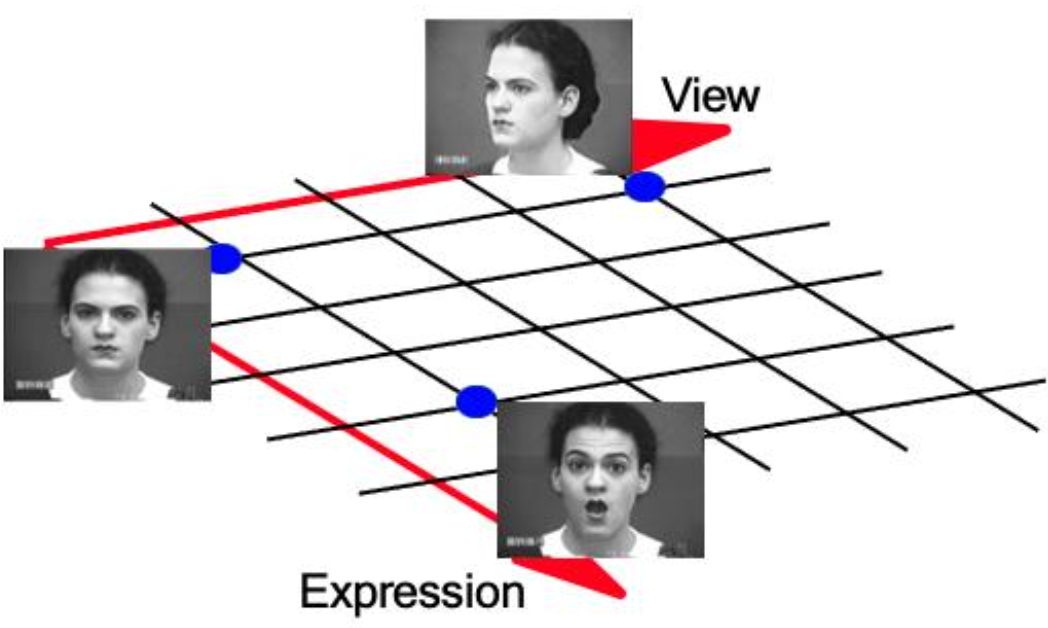
\includegraphics[width=0.45\linewidth]{figure/cartesianFig.png}
    \caption{Rappresentazione di una possibile idealizzazione su un piano cartesiano di un estrattore di features}
    \label{fig:cartesianFig}
\end{figure}
\section{Struttura Gerarchica dei Dati}
Le architetture multilivello riflettono la natura composizionale dei dati, analizzando le parti di esse di volta in volta, queste possono diventare delle ottime possibilità per spostarci verso un estrattore ideale, permettendo un'efficiente rappresentazione delle informazioni:

\begin{itemize}
    \item \textbf{Visione}: pixel $\Rightarrow$ bordi $\Rightarrow$ texture $\Rightarrow$ oggetti
    \item \textbf{Testo}: caratteri $\Rightarrow$ parole $\Rightarrow$ frasi $\Rightarrow$ discorso
    \item \textbf{Audio}: campioni $\Rightarrow$ bande spettrali $\Rightarrow$ fonemi $\Rightarrow$ parole
\end{itemize}

\section{Conclusione}
Le reti neurali profonde pertanto non fanno altro che bilanciare tempo e spazio, facendo sì che più livelli implicano più operazioni sequenziali, riducono la necessità di risorse computazionali parallele e infine consentono una rappresentazione più compatta delle funzioni complesse.
\chapter{Funzioni di attivazione}\label{chpt:5}
Le funzioni di attivazione sono molto importanti nelle reti neurali, in quanto introducono la non-linearità nel modello, permettendo di apprendere relazioni complesse nei dati. Senza funzioni di attivazione, una rete neurale profonda risulterebbe equivalente a una semplice trasformazione lineare.

\section{Vanishing Gradient Problem}
Uno dei problemi nell'addestramento delle reti neurali profonde è il \textbf{Vanishing Gradient Problem}, una problematica che viene a verificarsi, quando il gradiente venendo propagato all'indietro diventa molto piccolo, a causa di ciò, smetterà di imparare. È un problema frequente nell'utilizzare funzioni di attivazione come la \textbf{sigmoide} e la \textbf{tangente iperbolica}, poiché visionando i loro grafici, possiamo notare come ci siano grandi tratti dedicati al valore zero e al valore unitario. A causa di questa polarizzazione, i valori non si distinguono fra loro in maniera netta, pertanto tenderanno a scomparire.

\begin{figure}[h]
    \centering
    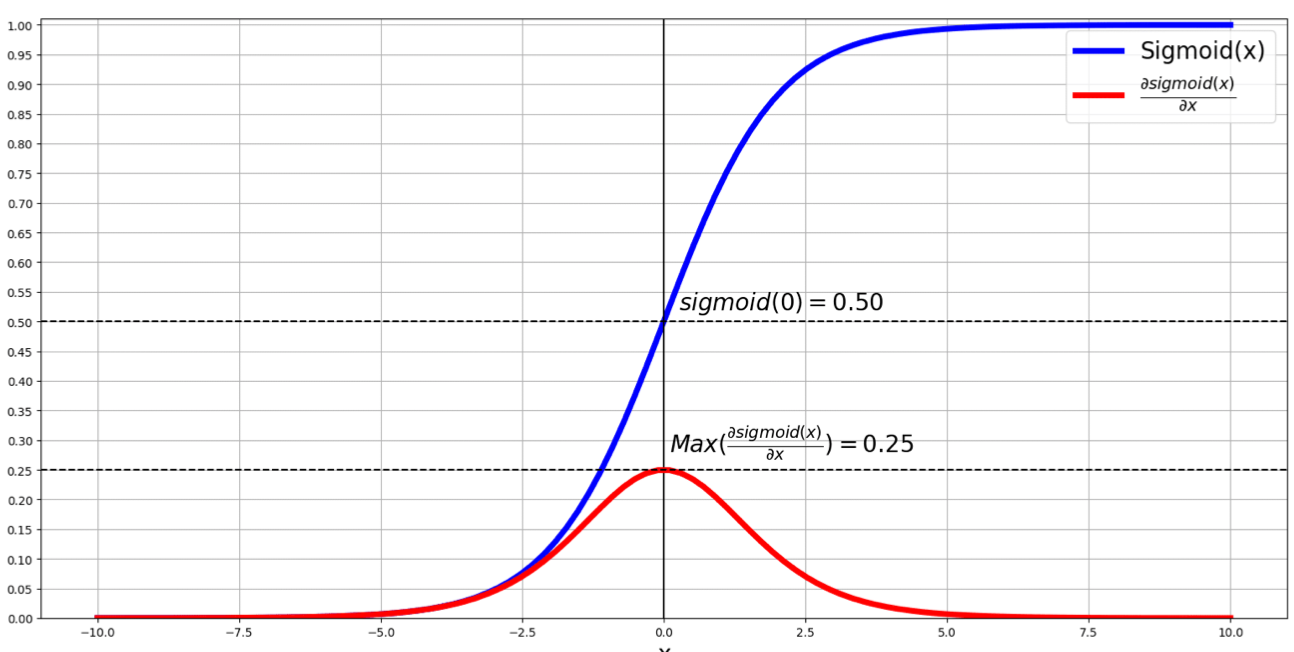
\includegraphics[width=0.85\textwidth]{figure/VanishingGradientProblem.png}
    \caption{Grafico descrittivo del Vanishing Gradient Problem, come possiamo vedere la derivata (in rosso) risulta essere molto ridotta per la gran parte dei valori.}
\end{figure}

\section{Funzioni non saturanti}
Per risolvere il problema, vengono utilizzate funzioni di attivazione dette \textbf{non-saturanti}, come:
\begin{itemize}
    \item \textbf{ReLU (Rectified Linear Unit):} elimina i valori negativi rendendo i calcoli più efficienti, crea però dei problemi legati al gradiente dei valori negativi, rendendoli tutti uguali e anche una mancata derivabilità nell'origine;
    \begin{equation}
        \operatorname{ReLU}(x) = \max(0, x)
    \end{equation}
    \item \textbf{Leaky ReLU:} introduce una piccola pendenza per i valori negativi, riuscendo a ridurre il problema creatosi con la \textit{ReLU};
    \begin{equation}
        \operatorname{LeakyReLU}(x) = \max(\alpha x, x)
    \end{equation}
    \item \textbf{PReLU (Parametric ReLU):} simile a Leaky ReLU, unica differenza è la pendenza dei valori negativi, il quale viene appreso durante l'addestramento, permettendo di avere una pendenza più incisiva;
    \item \textbf{RReLU (Randomized ReLU)}: la pendenza anche qui viene appresa durante l'addestramento, ma si basa su una variabile casuale.
\end{itemize}

\begin{figure}[h]
    \centering
    \begin{tikzpicture}
        \begin{axis}[xlabel={$x$}, ylabel={$f(x)$}, legend pos=north west, domain=-5:5, samples=100, grid]
            \addplot[color=deepblue, thick] {max(0,x)}; \addlegendentry{ReLU}
            \addplot[color=cadmiumorange, thick] {x >= 0 ? x : 0.01*x}; \addlegendentry{Leaky ReLU}
            \addplot[color=deepgreen, thick] {x >= 0 ? x : 0.1*x}; \addlegendentry{PReLU}
        \end{axis}
    \end{tikzpicture}
    \caption{Grafico di ReLU, Leaky ReLU e PReLU, tutti e tre i grafici dopo l'origine si sovrappongono, e seguono lo stesso andamento.}
\end{figure}

\section{Funzioni di Attivazione Avanzate}
Oltre alle funzioni non saturanti, esistono altre funzioni di attivazione avanzate, le quali puntano a gestire diversamente il problema dell'appiattimento dei valori negativi e della non differenziabilità nel punto di coordinata zero:
\begin{itemize}
    \item \textbf{ELU (Exponential Linear Unit):} permette l'utilizzo di valori negativi tramite una decrescita esponenziale, migliorando la stabilità;
    \item \textbf{SELU (Scaled ELU):} nei valori positivi lavora esattamente come una funzione lineare scalata, mentre per quelli negativi si ricurva gradualmente, come succede nella ELU, tuttavia utilizzando un fattore di scala, permettendo di prevenire che i neuroni diventino inattivi;
    \item \textbf{GELU (Gaussian Error Linear Unit):} utilizza una distribuzione gaussiana, utilizzata moltiplicandola per i valori ottenuti e avere delle transizioni più fluide fra i valori positivi e negativi;
    \item \textbf{Softplus}: è un'approssimazione allisciata della funzione rampa vista precedentemente grazie alla funzione non saturante ReLU, la quale permette di avere delle transizioni più dolci.
\end{itemize}

\begin{figure}[h]
    \begin{subfigure}{0.35\textwidth}
        \begin{tikzpicture}[scale=0.65]
            \begin{axis}[xlabel={$x$}, ylabel={$f(x)$}, domain=-5:5, samples=100,grid]
                \addplot[color=deepblue, thick] {x >= 0 ? x : (exp(x)-1)};
                \addplot[color=deepred, thick] {x >= 0 ? x : 1.05*(exp(x)-1)};
            \end{axis}
        \end{tikzpicture}
        \caption{ELU e SELU}
    \end{subfigure}
    \qquad\qquad\quad
    \begin{subfigure}{0.35\textwidth}
        \begin{tikzpicture}[scale=0.65]
            \begin{axis}[xlabel={$x$}, ylabel={$f(x)$}, domain=-5:5, samples=100,grid]
                \addplot[color=deepgreen, thick] {x >= 0 ? x : (exp(x)-1)};
                \addplot[color=cadmiumorange, thick] {0.5*x*(1+tanh(sqrt(2/pi)*(x+0.044715*x^3)))};
            \end{axis}
        \end{tikzpicture}
        \caption{CELU e GELU}
    \end{subfigure}
    \caption{Nel grafico sono rappresentate le varie funzioni di attivazione avanzate, a sinistra, vi è il confronto fra ELU (in blu) e SELU (in rosso), a destra invece il confronto fra CELU (in arancione) e GELU (in verde).}
\end{figure}

Tutte queste funzioni di attivazione, permettono di avere un taglio non netto, fra valori negativi e positivi, garantendo una similarità fra i valori presenti prima e dopo l'origine.

\section{Funzioni Normalizzanti}
Oltre alle moderne funzioni non saturanti, che sono diventate lo standard nella maggior parte delle reti profonde, esiste un'altra categoria di funzioni storicamente importanti o utilizzate in contesti specifici. A differenza delle funzioni come ReLU, il cui scopo principale è introdurre non-linearità mitigando il problema dei gradienti che svaniscono, le funzioni che seguono sono progettate per limitare i valori di output in modi molto specifici. Sebbene alcune di esse, come la funzione soglia (Treshold), siano oggi computazionalmente superate per l'addestramento di reti profonde, la loro comprensione è utile sia dal punto di vista storico sia perché i loro concetti di base riemergono in contesti più avanzati, come la regolarizzazione e l'elaborazione dei segnali.

\begin{itemize}
    \item \textbf{Hardtanh:} la $\operatorname{tanh}$ ha una curva a forma di "S" che si avvicina asintoticamente a $-1$ e $+1$, la $\operatorname{Hardtanh}$ sostituisce questa curva con una funzione lineare a tratti. È una retta con pendenza 1 nell'intervallo $[-1, 1]$ e assume valori costanti al di fuori di questo intervallo. Evita il calcolo di funzioni esponenziali, e sebbene saturi in valori al di fuori dell'intervallo la transizione è netta e non graduale, il che in alcuni contesti può aiutare a gestire meglio il problema dei gradienti che svaniscono;
    \item \textbf{Threshold:} Questa è la funzione di attivazione più semplice e storicamente, la prima ad essere stata utilizzata, fra gli anni '60 e '70, ispirata al modello "tutto o niente" del neurone biologico. Essendo la sua derivata zero, praticamente ovunque, è stata immediatamente rigettata per gli studi sulle rete neurali profonde;
    \item \textbf{Shrink Functions (Tanhshrink, Softshrink, Hardshrink):} Queste funzioni non sono tipicamente usate come attivazioni principali negli strati nascosti, ma piuttosto in contesti di regolarizzazione, sparse coding (codifica sparsa) o elaborazione dei segnali. Il loro scopo è quello di "contrarre" (shrink) i valori di input verso lo zero, eliminando o riducendo il "rumore" di bassa ampiezza.
\end{itemize}

\section{Funzioni Probabilistiche}
Fino ad ora, abbiamo analizzato funzioni di attivazione che operano in modo scalare, ovvero trasformano l'output di ogni singolo neurone indipendentemente dagli altri. Esiste, tuttavia, una classe di funzioni che opera a livello vettoriale, trasformando un intero vettore di output in una distribuzione di probabilità. Queste funzioni sono fondamentali nello strato di output dei modelli di classificazione multiclasse, dove l'obiettivo non è semplicemente ottenere un punteggio per ogni classe, ma interpretare questi punteggi come la probabilità che l'input appartenga a ciascuna di esse. Convertendo i valori grezzi del modello (logits) in probabilità, possiamo non solo selezionare la classe più probabile, ma anche quantificare la fiducia del modello nella sua previsione.

\begin{itemize}
    \item \textbf{Softmax:} questa funzione di attivazione trasforma un vettore in una distribuzione di probabilità all'interno di un range, essa inoltre enfatizza le differenze assegnando a valori più grandi una probabilità più alta, mentre quelli piccoli vengono schiacciati vicino allo zero, la somma di tutti i valori è pari a 1 amplificando la differenza fra i valori scalandoli a elementi dopo la virgola;
    \begin{equation}
        \operatorname{Softmax}(x_i) = \frac{e^{x_i}}{\sum_je^{x_j}}
    \end{equation}
    \item \textbf{Softmin:} la differenza rispetto alla Softmax è l'utilizzo del segno meno all'esponente, dunque una semplice inversione. Questo fa sì che valori più piccoli abbiano una probabilità maggiore, mentre i valori più grandi abbiano probabilità più piccole, essa inoltre è simmetrica rispetto al softmax;
    \begin{equation}
        \operatorname{Softmin}(x_i) = \frac{e^{-x_i}}{\sum_je^{-x_j}}
    \end{equation}
    \item \textbf{LogSoftmax:} quest'altra tipologia di funzione di attivazione invece è una variante della Softmax, in cui si applica il logaritmo alla funzione Softmax per migliorare la stabilità numerica e semplificare il calcolo della perdita nelle reti neurali.
    \begin{equation}
        \operatorname{LogSoftmax}(x_i) =\log( \frac{e^{x_i}}{\sum_je^{x_j}})
    \end{equation}
\end{itemize}

\begin{Osservazione}
    La funzione Softmax può essere vista come la generalizzazione della funzione Sigmoide dal caso binario al caso multiclasse. In altre parole, la Sigmoide è un caso speciale di Softmax quando le classi da predire sono solo due ($K=2$).
\end{Osservazione}

\chapter{Loss Function}
Una \textbf{funzione di costo} (o loss function) è un elemento fondamentale nel Deep Learning, perché misura \textit{quanto è sbagliata la predizione di un modello} rispetto ai valori reali. L'obiettivo dell'apprendimento automatico è quello di minimizzare questa funzione, in modo che il modello faccia previsioni più accurate, la misurazione delle funzioni di costo, come abbiamo già detto in precedenza è fondamentale per un criterio valutativo, ma anche per effetuarvi la Backpropagation nelle reti neurali.
\section{MSE Loss}
La funzione \texttt{nn.MSELoss()} calcola l'errore quadratico medio (MSE) tra le predizioni e i valori target, questa tipologia di funzione di costo utilizza la L2 Norm:
\begin{equation}
L = \frac{1}{N} \sum_{i=1}^{N} (x_i - y_i)^2
\end{equation}
Questa funzione di costo è sensibile agli outlier poiché gli errori vengono elevati al quadrato.
\section{L1 Loss}
La \texttt{nn.L1Loss()} invece misura l'errore assoluto medio (MAE) tra le predizioni e i valori target, questa tipologia di funzione di costo utilizza la L1 Norm:
\begin{equation}
L = \frac{1}{N} \sum_{i=1}^{N} |x_i - y_i|
\end{equation}
Questa funzione di costo, rispetto alla precedente risulta essere più robusta agli outlier.
\section{L1 vs L2}
Ci si è chiesti pertanto quale delle due è maggiormente corretto utilizzare, si è giunti a delle considerazioni sulla base di visioni sperimentali. Infatti seguono due diversi comportamenti. Si è mostrato come il comportamento ottenuto con L2, qui tutti i valori vengono distribuiti uniformemente, mentre con L1 i risultati sono leggermente più netti. Questa caratteristica può essere visualizzata attraverso l'utilizzo di modelli di computer vision, infatti si è potuto verificare sperimentalmente come in effetti L1 sia migliore quando ci sono delle immagini più spigolose, diversamente otteniamo un risultato migliore con L2 in immagini che risultano essere più morbide nelle loro forme (Figura~\ref{fig:l1l2diff}).

\begin{figure}
    \centering
    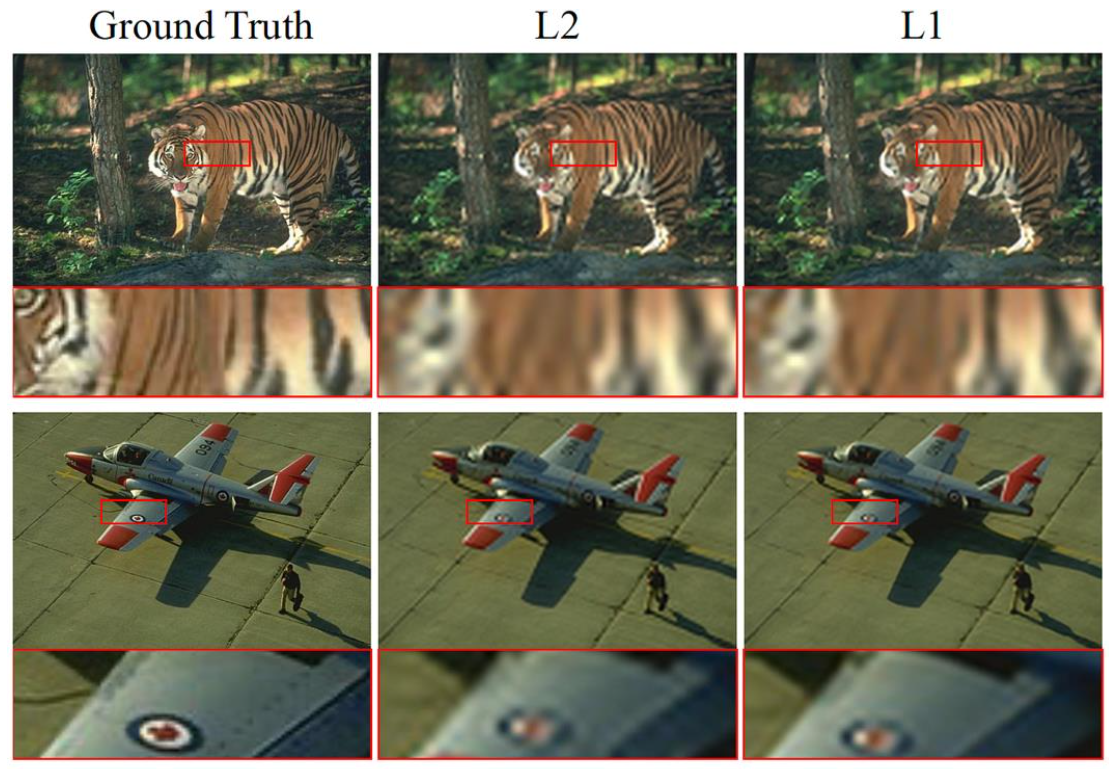
\includegraphics[width=0.75\linewidth]{figure/L1andL2.png}
    \caption{Utilizzando un modello di computer vision possiamo notare come è più accurata la norma 2 per figure meno spigolose, come quella della tigre, differentemente per l'immagine in cui vi è l'aereo la norma 1 è migliore poiché l'immagine risulta più spigolosa.}
    \label{fig:l1l2diff}
\end{figure}

\section{Smooth L1 Loss}
Per far sì che si trovi un equilibrio fra le due si è optato per creare una combinazione tra L1 e MSE per gestire gli outlier al meglio e la stabilità numerica, implementando la Smooth L1 Loss:
\begin{equation}
L(x, y) = \begin{cases} 
\frac{1}{2} (x - y)^2, & \text{se } |x - y| < 1 \\
|x - y| - \frac{1}{2}, & \text{altrimenti}
\end{cases}
\end{equation}

Qui pertanto abbiamo una combinazione delle due precedenti, in alcuni casi viene utilizzata la norma 2 in altri viene applicata la norma 1, favorendo un'ottimizzazione più netta.
\section{Negative Log Likelihood Loss}
La Negative Log Likelihood Loss (NLL Loss) è una funzione di costo comunemente usata nei problemi di classificazione multi-classe, soprattutto quando l'output del modello è espresso in log-probabilità (tramite LogSoftMax). Quando il dataset risulta essere sbilanciato, la NLL Loss tende a favorire le classi più frequenti, portando il modello a ignorare quelle meno rappresentate. Per risolvere questo problema, si può modificare la NLL Loss aggiungendo pesi per ogni classe. Essa è definita come segue, la seguente equazione la mostra considerando quella media basata su N esempi:

\begin{equation}
    L = -\frac{1}{N}\sum^{N}_{i=1}\log P(y_i|x_i)
\end{equation}

\subsection{Problema delle classi sbilanciate}
Se un dataset risulta essere sbilanciato, il modello tenderà a imparare a minimizzare la loss predicendo sempre la classe più frequente.

\begin{Esempio}
    Se il dataset ha 90\% di classe A e 10\% di classe B, il modello potrebbe semplicemente predire sempre classe A per minimizzare la loss, portando a un'accuratezza apparente alta ma con prestazioni pessime per la classe B.
\end{Esempio}

La soluzione a questa possibilità, è quella di aggiungere ulteriori pesi alle classi nella NLL Loss. Il bilancaimento viene effettuato nel seguente modo:

\begin{equation}
    L = -\frac{1}{N}\sum^{N}_{i=1}w_{y_i}\log P(y_i|x_i)
\end{equation}

Introducendo molto semplicemente un peso $w_{y_i}$ a ogni classe. Valorizzando in maniera migliore la classe minoritaria, che altrimenti verrebbe inevitabilmente schiacciata dall'altra allenando dunque il nostro modello nella maniera scorretta. Aumentare i pesi però non è la stessa cosa di avere un dataset bilanciato, pertanto è necessario chiedersi quali potrebbero essere altre soluzioni che potremmo adottare per poter bilanciare i dati.

\section{Cross Entropy Loss}
La funzione \texttt{nn.CrossEntropyLoss()} combina \texttt{LogSoftmax} e \texttt{NLLLoss} in un'unica funzione ed è la più utilizzata nei problemi di classificazione multi-classe. La perdita di entropia incrociata è definita come:
\begin{equation}
L = - \sum_{i=1}^{N} \sum_{j=1}^{C} y_{i,j} \log(\hat{y}_{i,j})
\end{equation}
dove:
\begin{itemize}
    \item $C$ è il numero di classi,
    \item $y_{i,j}$ è 1 se l'osservazione $i$ appartiene alla classe $j$, altrimenti è 0,
    \item $\hat{y}_{i,j}$ è la probabilità predetta per la classe $j$.
\end{itemize}
L'entropia incrociata permette di misurare la distanza tra due distribuzioni di probabilità: quella vera dei dati e quella predetta dal modello. Più le due distribuzioni sono simili, più bassa è la perdita. Un valore alto della perdita indica che le probabilità predette si discostano fortemente dai valori reali. Un aspetto cruciale dell'entropia incrociata è la sua connessione con la \textit{divergenza di Kullback-Leibler} (KL). La KL-divergence misura quanto una distribuzione differisce da un'altra e può essere espressa come:
\begin{equation}
D_{KL}(P||Q) = \sum_{i} P(i) \log \frac{P(i)}{Q(i)}
\end{equation}
dove $P$ rappresenta la distribuzione reale e $Q$ quella predetta. La cross-entropy include implicitamente questa metrica, motivo per cui è così efficace nei problemi di classificazione.

\section{Adaptive Log Softmax with Loss}
Quando si hanno problemi con molte classi, l'uso di una softmax standard può essere inefficiente. Per questo motivo si introduce \texttt{nn.AdaptiveLogSoftmaxWithLoss()}, che suddivide le classi in gruppi gerarchici e riduce il costo computazionale.

\section{Binary Cross Entropy Loss}
Per problemi di classificazione binaria, MSE non è ideale perché non gestisce correttamente la probabilità logaritmica. Si introduce quindi la funzione \texttt{nn.BCELoss()}:
\begin{equation}
L = - \frac{1}{N} \sum_{i=1}^{N} -w_i\left[y_i \log({x}_i) + (1 - y_i) \log(1 - x_i) \right]
\end{equation}
Questa funzione penalizza maggiormente le previsioni errate con alta confidenza, risultando più efficace rispetto a MSE per la classificazione.

\section{Kullback-Leibler Divergence Loss}
BCELoss assume che la distribuzione target sia binaria, ma a volte vogliamo misurare quanto una distribuzione di probabilità predetta si discosti da quella reale. Per questo si usa la KL Divergence:
\begin{equation}
D_{KL}(P||Q) = \sum_{i} P(i) \log \frac{P(i)}{Q(i)}
\end{equation}
Questa misura è utile per modelli probabilistici come le reti neurali bayesiane.

\section{BCE Loss with Logits}
Un problema della BCE standard è che richiede l'utilizzo della funzione sigmoide in maniera separata, questo fattore potrebbe causare instabilità numerica. Per risolvere questo problema pertanto, la \texttt{nn.BCEWithLogitsLoss()} incorpora direttamente la sigmoide nella perdita.
\begin{equation}
    L = - \frac{1}{N} \sum_{i=1}^{N} -w_i\left[y_i \log(\sigma({x}_i)) + (1 - y_i) \log(1 - \sigma({x}_i) \right]
\end{equation}

\section{Hinge Embedding Loss}
Quando si lavora con problemi di similarità (es. metric learning), vogliamo una funzione di costo che enfatizzi la distanza tra esempi simili e dissimili. \texttt{nn.HingeEmbeddingLoss()} è utile in questi casi. Infatti se la nostra distanza è inferiore a un certo limite otterrò la selezione all'interno di un valore dando come risultato un valore, alternativamente avrò come esito un altro.

\section{Margin Ranking Loss}
Simile alla Hinge Loss, ma si usa in compiti di ranking dove dobbiamo garantire che un elemento corretto abbia punteggio più alto rispetto a un elemento errato, questo ci permette al nostro sistema di ordinare qualcosa al meglio.
\begin{equation}
    L = \max(-y\,(x_1-x_2)+\text{margin},\,0) 
\end{equation}

\section{Triplet Margin Loss}
Per migliorare la distinzione tra classi, \texttt{nn.TripletMarginLoss()} è ciò che viene utilizzato, questa confronta un'ancora, con un esempio positivo e uno negativo, questo ci permette anche di considerare più di due singole categorie:
\begin{equation}
L = \max(0, d(a, p) - d(a, n) + \text{margin})
\end{equation}
Questa funzione risulta essere cruciale per l'apprendimento di embedding robusti, come nel riconoscimento facciale.

\section{Soft Margin Loss}
Una variante della Hinge Loss che introduce una penalità logistica per evitare margini rigidi:
\begin{equation}
L = \sum_{i=1}^{N} \log(1 + e^{-y_i x_i})
\end{equation}

Questa funzione di costo non fa altro che integrare la funzione di softmax, a quella logistica, volendo fare in modo che i valori positivi siano più vicini fra loro e spingeranno i valori negativi lontani aggiungendo un decadimento esponenziale alla funzione di costo.

\section{Multi-Class Hinge Loss}
Quando abbiamo più di due classi, una semplice Hinge Loss non è sufficiente. \texttt{nn.MultiLabelMarginLoss()} estende il concetto a problemi multi-classe. 

\section{Cosine Embedding Loss}
Giungiamo ora all'ultima funzione di costo, nel nostro caso partiamo prendendo in considerazione un esempio partendo da delle frasi, immaginiamo che vogliamo creare una situazione in cui le frasi con lo stesso significato, possano essere legate, e se avessimo diverse frasi vogliamo trovare un modo per valutare se stanno parlando della stessa cosa o meno. Sicuramente se abbiamo due frasi diverse verranno poste in posizioni diverse nel nostro spazio latente, anche se sono leggermente diverse e parlano dello stesso contesto. Tuttavia se abbiamo la necessità di unificarle, rischiamo di perdere informazioni appiattendo la varietà di linguaggio basata su tono, espressività, gergo, ecc\dots
\begin{figure}[h]
    \centering
    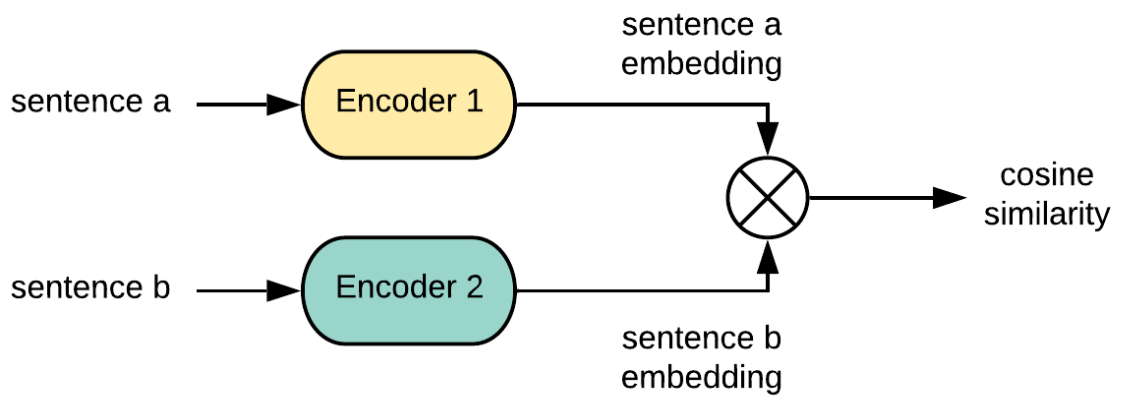
\includegraphics[width=0.75\linewidth]{figure/CosineSim.png}
    \caption{Rappresentazione di come che vorrei trattare due frasi per determinarne la loro similarità}
    \label{fig:coSim}
\end{figure}
Ciò che i ricercatori sono riusciti a capire che due parole seguono lo stesso vettore, sebbene siano leggermente differenti, possiamo fare ciò attraverso la \textbf{Cosine similarity}. Ossia si calcola il coseno dell'angolo compreso fra due vettori. Se i due vettori sono uguali fra loro la risposta sarà zero differentemente non lo sarà.
\begin{Osservazione}
    Se due vettori sono completamente diversi fra loro, idealmente i due vettori saranno posizionati ortogonalmente fra loro.
\end{Osservazione}
    
Per misurare la similarità tra vettori in uno spazio di embedding, si usa la \texttt{nn.CosineEmbeddingLoss()}:
\begin{equation}
L = \begin{cases} 
1 - \cos(x_1, x_2), & \text{se } y = 1 \\
\max(0, \cos(x_1, x_2) - \text{margin}), & \text{se } y = -1
\end{cases}
\end{equation}
\\
Questa funzione risulta essere fondamentale nei sistemi di retrieval e riconoscimento facciale.
\chapter{Ottimizzazione}
Una delle parti più importanti del Deep Learning è quella legata alla parte di \textbf{Ottimizzazione}. Fino ad ora, noi conosciamo lo 	\textbf{Stochastic Gradient Descent}, sappiamo però che molto spesso implementandolo attraverso le sue varianti (Batch, MiniBatch, ecc\dots), si possono incontrare diversi problemi nell'allenare il modello. Dunque, questo capitolo ha lo scopo di andare oltre queste metodologie tradizionali per ottimizzare il nostro modello. La superficie d'errore in cui ci ritroviamo può essere rappresentata da una parabola o, in più dimensioni, da una sfera. Tuttavia, nella pratica, le nostre curve di errore assumono la forma di ellissi, poiché le scale delle varie feature sono diverse fra loro (Figura~\ref{fig:error_surface}). Pertanto, la discesa del gradiente diventa inefficiente, subendo rallentamenti e oscillazioni, che ne compromettono la convergenza.

\begin{figure}[h]
\centering
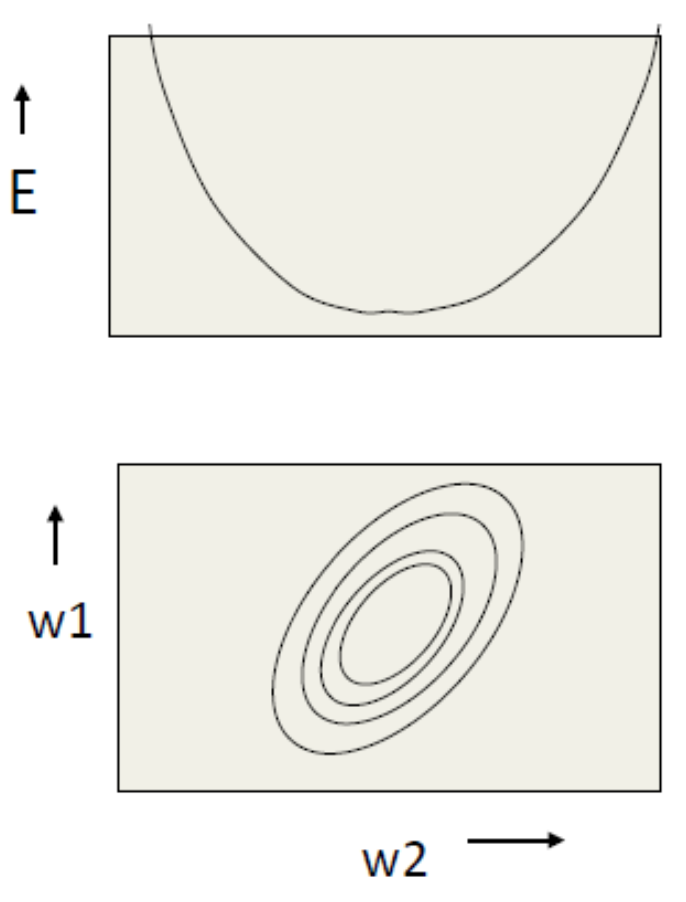
\includegraphics[width=0.55\textwidth]{figure/error_surface.png}
\caption{Rappresentazione della superficie d'errore}
\label{fig:error_surface}
\end{figure}

\section{Discesa del Gradiente}
Se il dataset risulta essere altamente ridondante, il gradiente nella prima metà dei dati sarà praticamente identico a quello presente nella seconda metà. Dunque, invece di calcolare l'intero gradiente, possiamo computarlo solo su una porzione dei dati e riutilizzarlo sulla restante parte. L'idea successiva a questa considerazione, è quella di utilizzare piccoli batch dell'intero dataset in modo tale che essi siano rappresentativi delle classi in analisi. Questo porta all'uso della discesa del gradiente stocastica con mini-batch, una soluzione che migliora l'efficienza computazionale e la stabilità dell'addestramento.

\subsection{Scegliere il learning rate}
Per poter scegliere il learning rate, inizialmente decidiamo di impostarlo a un valore elevato, in modo tale da evitare di collassare su un minimo locale troppo presto. Successivamente, attraverso tecniche di decay, lo riduciamo progressivamente per aumentare la probabilità di convergere verso un minimo globale o comunque un minimo locale migliore rispetto a quelli precedenti. Tra le strategie più comuni per il decay del learning rate possiamo considerare le seguenti:
\begin{itemize}
\item\textbf{Step Decay}: il learning rate viene ridotto di un fattore fisso dopo un certo numero di epoche;
\item\textbf{Exponential Decay}: il learning rate diminuisce esponenzialmente nel tempo;
\item\textbf{Adaptive Learning Rate}: tecniche come Adam e RMSprop regolano dinamicamente il learning rate per ogni parametro della rete.
\end{itemize}

\begin{figure}[!ht]
    \centering
    \begin{tikzpicture}[scale=0.8]
        \begin{axis}[
            width=12cm, height=7cm,
            xlabel={Epochs},
            ylabel={Learning Rate},
            xmin=0, xmax=50,
            ymin=0, ymax=0.12,
            legend style={
                at={(0.5,1.2)},
                anchor=north,
                legend columns=3
            },
            xtick={0,10,20,30,40,50},
            ytick={0.02,0.04,0.06,0.08,0.1,0.12},
            grid=both,
            thick,
            every axis plot/.append style={line width=1pt},
        ]

        % Step decay
        \addplot[blue, domain=0:50, samples=51] 
            {0.1 * (x<10 ? 1 : (x<30 ? 0.05 : 0.025))};
        \addlegendentry{Step Decay}

        % Exponential decay
        \addplot[red, domain=0:50, samples=200]
            {0.1 * exp(-0.05*x)};
        \addlegendentry{Exponential Decay}

        % Adaptive (manually simulated)
        \addplot[green!60!black, mark=*] 
            coordinates {
                (0, 0.1) (5, 0.1) (10, 0.09) (15, 0.09)
                (20, 0.06) (25, 0.06) (30, 0.045)
                (35, 0.045) (40, 0.03) (45, 0.03) (50, 0.02)
            };
        \addlegendentry{Adaptive Learning Rate}

        \end{axis}
    \end{tikzpicture}
    \caption{Confronto tra diverse strategie di decadimento del learning rate.}
    \label{fig:lr_decay}
\end{figure}

\subsection{Inizializzazione dei pesi}
Un altro problema rilevante riguarda l'inizializzazione dei pesi nelle reti neurali. A differenza della regressione lineare, in cui l'ottimizzazione è più diretta, nelle reti neurali l'algoritmo di backpropagation può essere compromesso se i pesi iniziali non sono scelti correttamente. Se due pesi all'interno di uno stesso layer hanno valori iniziali identici, l'errore propagato attraverso la rete genererà aggiornamenti identici per entrambi, portando dunque alla simmetria dei pesi, questo impedirà alla rete di apprendere in maniera efficiente. Inoltre, se i pesi sono inizializzati con valori troppo grandi o troppo piccoli, si possono verificare problemi di vanishing o exploding gradient o ancora il problema dell'overshoot in cui non si giunge a convergenza, ma vi è un'oscillazione continua dei valori.

\subsubsection{Fan-in e Fan-out}
\marginpar{\href{https://proceedings.mlr.press/v9/glorot10a/glorot10a.pdf}{"Understanding the difficulty of training deep feedforward neural networks" by Xavier Glorot et al. (2010)~\cite{glorot2010understanding}}}
Il Fan-In e il Fan-Out sono concetti legati alla distribuzione dei pesi negli strati di una rete neurale e vengono usati in tecniche di inizializzazione dei pesi come quella Xavier (Glorot).
\begin{itemize}
    \item \textbf{Fan-in}: il numero di neuroni che alimentano un dato neurone in un layer successivo;
    \item\textbf{Fan-out}: il numero di neuroni che un dato neurone alimenta nel layer successivo;
\end{itemize}

\begin{Esempio}
    Consideriamo un layer completamente connesso (fully connected, FC) con: 256 neuroni in ingresso, dunque il fan-in sarà 256, e con 512 neuroni in uscita, dunque il fan-out sarà 512.
\end{Esempio}


L'inizializzazione dei pesi deve tener conto di questi valori per evitare che le attivazioni diventino troppo grandi o troppo piccole. Tecniche come Xavier prendono in considerazione questi aspetti, utilizzando distribuzioni gaussiane o uniformi adeguate. Basti pensare che nel momento in cui inizializiamo i pesi in maniera casuale, se venissero scelti con una varianza troppo grande, i valori dell'attivazione esplodono strato dopo strato (exploding activations). Se la varianza è troppo piccola, i segnali si riducono progressivamente (vanishing activations), rendendo difficile l'apprendimento.

\subsection{Xavier Initialization}
L’idea chiave della \textbf{Xavier Initialization} è scegliere i pesi in modo tale che:
\begin{enumerate}
    \item La varianza dell'output di un neurone sia simile alla varianza del suo input (per evitare esplosioni o annullamenti del segnale);
    \item La varianza dei gradienti rimanga costante tra gli strati (per evitare la degenerazione del training);
\end{enumerate}
Consideriamo $x$ l'input di un neurone e $W$ il vettore dei suoi pesi, l'output del neurone pertanto sarà dato da $z=Wx$, se supponiamo che $x$ abbia media nulla e varianza $\operatorname{Var}[x]$, allora la varianza del nostro output sarà chiaramente $\operatorname{Var}[Wx]$. Se assumiamo che i pesi e gli input siano indipendenti fra loro e che i pesi abbiano media nulla e varianza $\sigma^2$ otteniamo che la varianza sarà $\operatorname{Var}[z]=n_{in}\sigma^2\operatorname{Var}[x]$, dove ricordiamo come $n_{in}$ sia il fade-in. Se vogliamo mantenere la varianza costante tra gli strati ci basta imporre che $n_{in}\sigma^2=1$, in questo modo ricavo facilmente $\sigma^2=\frac{1}{n_{in}}$, e ovviamente riuscendo a ricavare il valore della deviazione standard, questo mi suggerisce che i valori possano seguire una distribuzione normale a media nulla e deviazione standard calcolata:
\begin{equation}
    \mathcal{N}\left(0,\,\frac{1}{n_{in}}\right)
\end{equation}

Se volessimo aggiungere la correlazione con il fan-out rendendo l'assegnazione più robusta la aggiungeremo al denominatore della deviazione standard come segue:
\begin{equation}
       \mathcal{N}\left(0,\,\frac{1}{n_{in}+n_{out}}\right) 
\end{equation}
 
oppure in maniera più semplice possiamo utilizzare una distribuzione uniforme la quale sarà ottenuta come segue:
\begin{equation}
    \mathcal{U}\left(-\frac{\sqrt{6}}{\sqrt{n_{in}+n_{out}}},\,\frac{\sqrt{6}}{\sqrt{n_{in}+n_{out}}}\right)
\end{equation}

La Xavier Initialization risulta essere un miglioramento rispetto all'inizializzazione a zero o quella casuale arbitraria, perché bilancia la propagazione del segnale nei vari strati. Tuttavia, non è sempre ideale per funzioni di attivazione non lineari come ReLU, per cui esiste una variante chiamata \textit{He initialization} che utilizza un 2 al numeratore nella distribuzione gaussiana.

\subsection{Correlazione fra le Features}
Per normalizzare i dati, possiamo utilizzare tecniche come la \textit{min-max normalization} e la \textit{z-score normalization}, che rendono il dataset più coerente e scalabile. Tuttavia, queste tecniche assumono che le feature siano scorrelate, un'ipotesi raramente valida nel mondo reale. Un obiettivo fondamentale è quindi quello di decorrelare gli input in modo efficace. Questo può essere ottenuto mediante:
\begin{itemize}
\item\textbf{Principal Component Analysis (PCA)}: una tecnica che trasforma le feature originali in nuove variabili non correlate;
\item\textbf{Whitening}: una trasformazione che rende le feature scorrelate e con varianza unitaria;
\item\textbf{Batch Normalization}: una tecnica che normalizza le attivazioni durante l'addestramento per migliorare la stabilità e accelerare la convergenza.
\end{itemize}

\begin{table}[!ht]
    \centering
    \caption{Confronto tra PCA, Whitening e Batch Normalization}
    \begin{adjustbox}{width=\textwidth}
    \begin{tabular}{@{} lccc @{}}
        \toprule
        \textbf{Caratteristica} & \textbf{PCA} & \textbf{Whitening} & \textbf{Batch Normalization} \\
        \midrule
        \textbf{Tipo} & Preprocessing & Preprocessing & In-training normalizzazione \\
        \textbf{Obiettivo} & Riduzione dimensionalità & Decorrelazione delle feature & Accelerare il training \\
        \textbf{Agisce su} & Intero dataset & Intero dataset & Mini-batch durante il training \\
        \textbf{Rende varianza uniforme?} & No & Sì (varianza unitaria) & No (mantiene varianza originale) \\
        \textbf{Rende feature ortogonali?} & Sì & Sì & No \\
        \textbf{Mantiene struttura dati?} & Parzialmente & Meno rispetto a PCA & Sì \\
        \textbf{Uso tipico} & Compressione dati, pretraining & Preprocessing per ICA, SVM & Normalizzazione nei layer di Reti Neurali \\
        \textbf{Effetto su reti neurali} & Riduce dimensionalità in input & Raramente usato direttamente & Migliora stabilità e velocità di training \\
        \bottomrule
    \end{tabular}
    \end{adjustbox}
\end{table}

\section{Momentum}
Come abbiamo visto durante il corso di Machine Learning l'algoritmo più semplice per l'aggiornamento dei pesi è la discesa del gradiente standard, essa aggiorna un peso $w$ seguendo la direzione negativa del gradiente della funzione di costo nella seguente maniera :
\begin{equation}
    w_{t+1} = w_t - \eta\frac{\partial J}{\partial w_t} 
\end{equation}

Il problema che viene a verificarsi in questo caso è la convergenza lenta, se la funzione di costo ha una superficie irregolare, come in una valle stretta e lung, il gradiente può essere molto grande in una direzione e molto piccolo in un'altra. Questo causerà delle oscillazioni, invece di una discesa verso il minimo.

\begin{Esempio}
    Immaginiamo di far rotolare una pallina giù per una montagna con una valle molto stretta. Se muovo la pallina solo in base alla pendenza locale, questa potrebbe oscillare avanti indietro nella valle, invece di muoversi rapidamente verso il basso e poi fermarsi.
\end{Esempio}

Il \textbf{Momentum} risolve infatti questa problematica accumulando la storia dei gradienti precedenti, aggiungendo un termine di velocità che aiuta a mantenere il movimento nella direzione giusta e a smorzare le oscillazioni, dunque adesso non avrò più una singola iterazione, ma ben due:

\begin{equation}
    \left\{\begin{array}{c}
    p_{k+1} = \beta p_k + \eta\,\nabla L(X,\,y,\,w_k)
    \\
    w_{k+1} = w_k - \gamma\,p_{k+1}
    \end{array}\right.
\end{equation}
\\
In questo caso $p$ sarebbe il \textit{Momentum Parameter} il quale prende in analisi la velocità di discesa fino a un determinato momento, mentre $\beta$ è il così detto \textit{Damping Factor}, un valore che controlla quanto la velocità passata influenza quella attuale, compreso fra zero e uno, se fosse zero, staremmo facendo semplicemente la discesa del gradiente, mentre se fosse uno avrei un'esplosione del gradiente nella nostra rete neurale. Il valore del damping factor, ci permette di vedere come più piccolo è più il cambio di direzione è veloce.

\begin{figure}[ht]
    \centering
    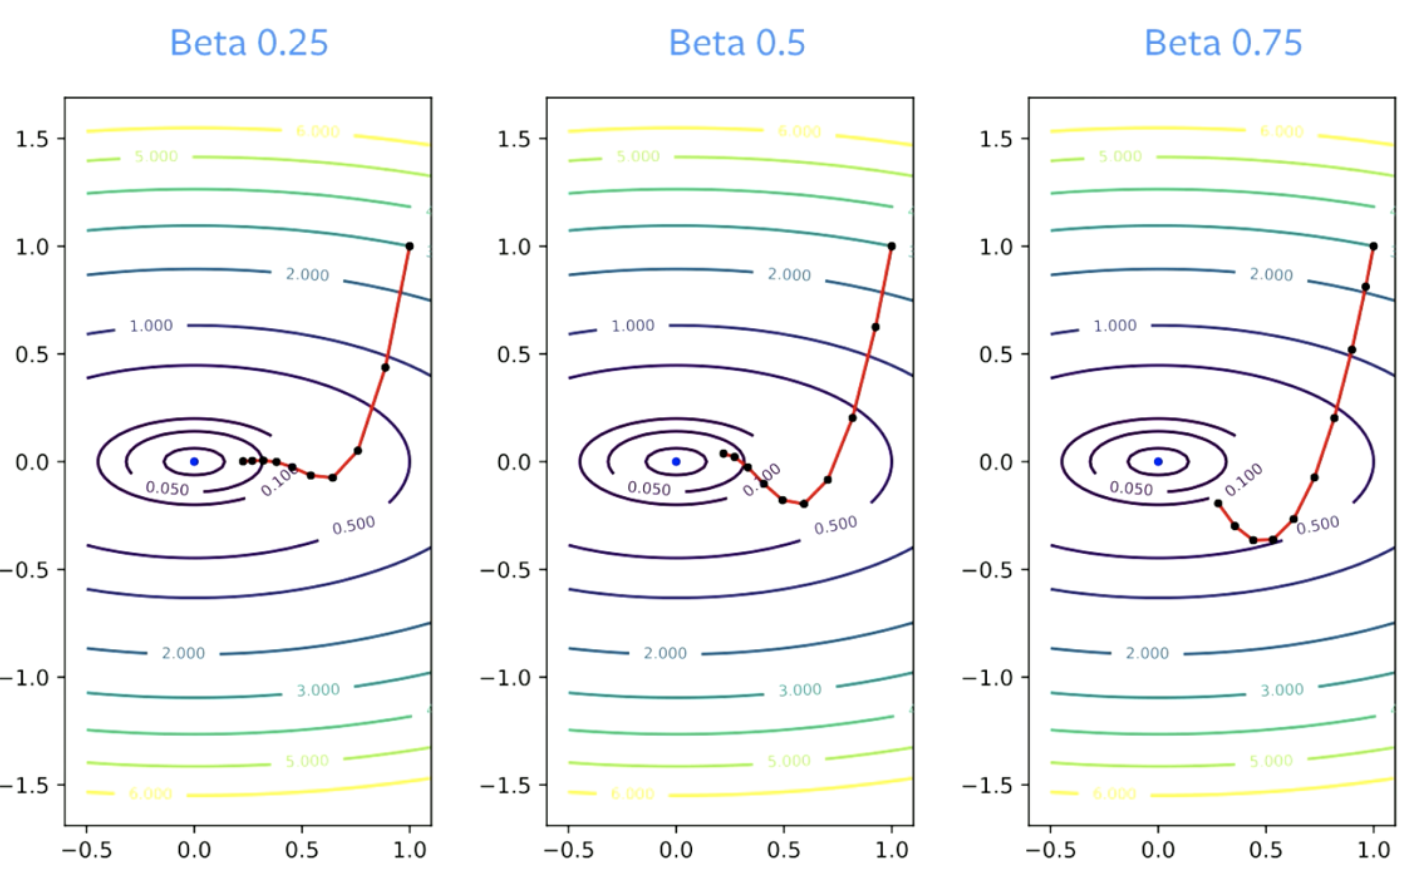
\includegraphics[width=\textwidth]{figure/DampingFactMomentum.png}
    \caption{Confronto delle traiettorie per diversi valori di $\beta$ nel Momentum}
\end{figure}

\section{Nesterov Accelerated Gradient}
Il Momentum classico aiuta la discesa del gradiente accelerando il processo e smorzando le oscillazioni, ma ha un problema: aggiorna i pesi basandosi sulla direzione del gradiente calcolato nella posizione attuale, senza considerare dove il peso si troverà dopo l'aggiornamento. Il matematico Yurii Nesterov nel 1983 propose una modifica intelligente al Momentum classico, chiamata \textbf{Nesterov Accelerated Gradient} (NAG), che migliora la velocità di convergenza e la stabilità dell’ottimizzazione. L'analogia possibile da effettuare è quella di una persona che va in bicicletta: quando usiamo il momentum classico, è come se spingessi forte sui pedali senza guardare avanti, basandomi solo sulla velocità che ho accumulato. Se la strada curva improvvisamente, potrei andare troppo veloce nella direzione sbagliata e dover correggere bruscamente. Con il momentum di Nesterov, invece, è come se guardassi avanti prima di spingere, capendo dove sto andando. Se vedessi che la strada curva, potrò correggere prima il mio movimento, evitando di andare fuori strada e pedalando in modo più intelligente.
\begin{figure}
    \centering
    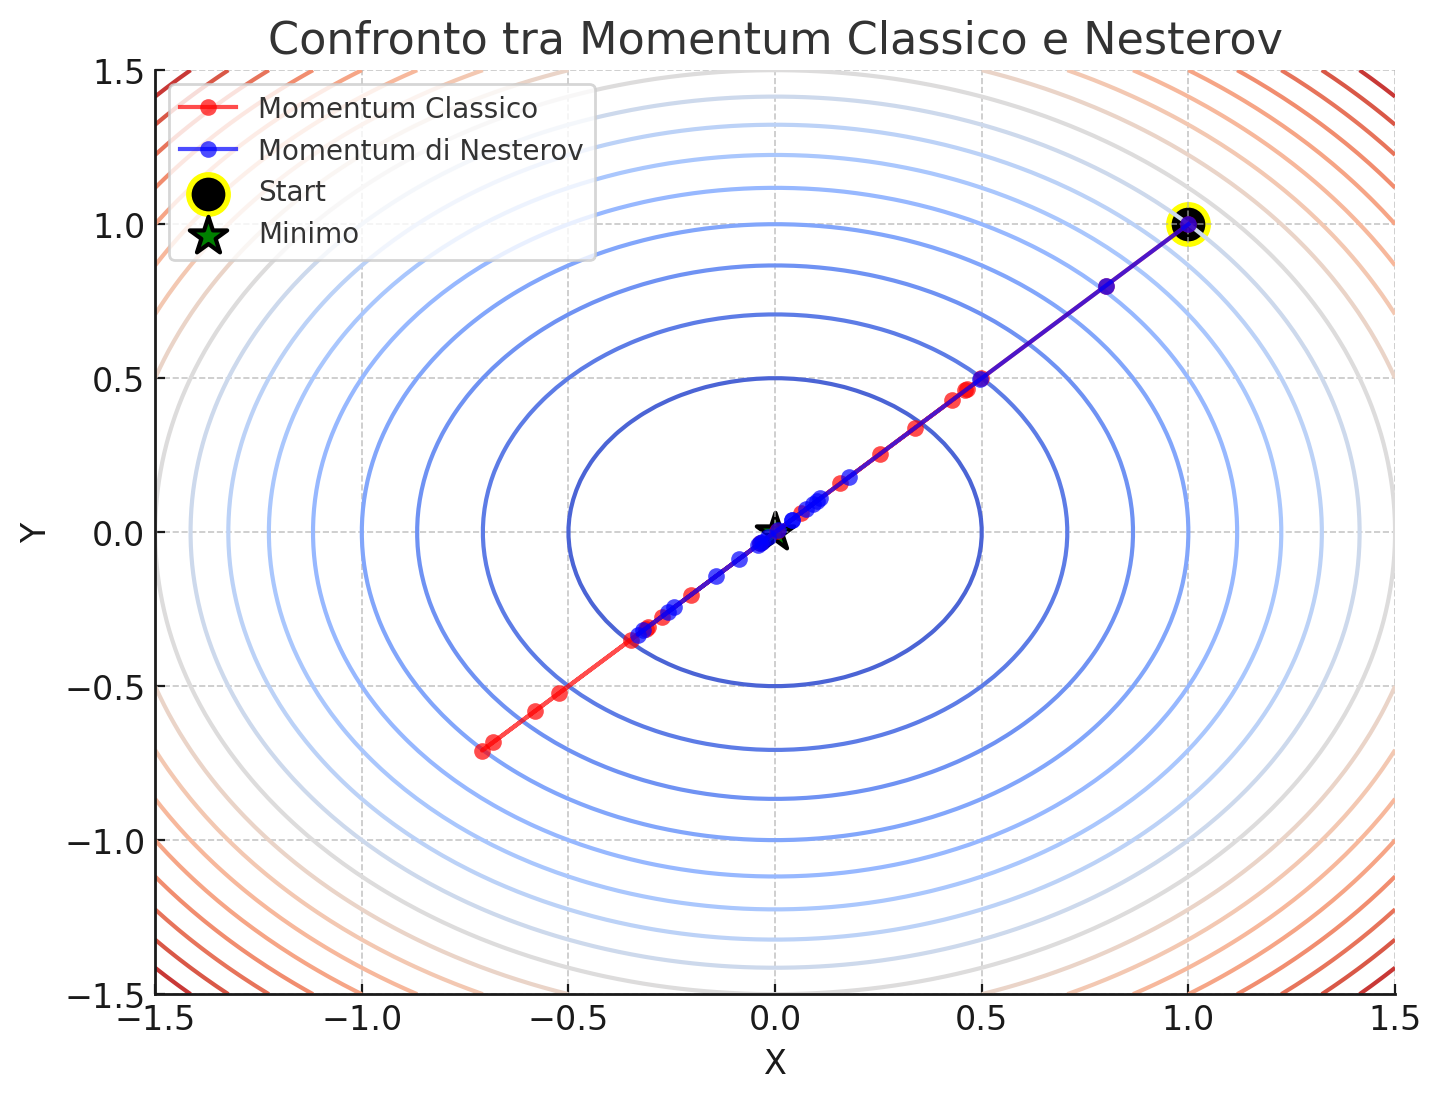
\includegraphics[width=0.75\textwidth]{figure/momenest.png}
    \caption{Nel grafico è possibile vedere la velocità di convergenza confrontando i due Momentum entrambi partendo da uno stesso punto d'inizio, il Momentum classico come potevamo aspettarci avrà delle oscillazioni molto più grandi rispetto a quelle del Momentum di Nesterov.}
    \label{fig:MomentumVS}
\end{figure}
Pertanto come fa il Momentum di Nesterov a essere più efficiente, semplicemente calcolando il gradiente in una posizione successiva l'algoritmo ha un'idea di dove il peso sta andando, evitando overshooting, inoltre poiché il gradiente viene calcolato in una posizione più realistica, l'algoritmo può correggere la direzione prima di fare un grande aggiornamento. E infine Nesterov aiuta a mantenere un'alta velocità senza instabilità, specialmente in funzioni di costo con superfici curve e strette.

\begin{equation}
\left\{\begin{array}{c}
    p_{k+1} = \beta p_k\,+\,\eta\,\frac{\partial J}{\partial(w_k\,+\,\beta\,p_k)}\\
    w_{k+1} = w_k\,+\,v_{k+1}
    \end{array}\right.
\end{equation}

Nesterov è un piccolo ma potente miglioramento rispetto al Momentum classico. Questo metodo viene spesso usato negli ottimizzatori moderni come Adam, RMSprop con Momentum, e molte varianti di SGD, perché migliora stabilità e velocità di convergenza.

\subsection{Ma perché proprio funziona il Momentum ?}
Il Momentum funziona principalmente per due motivi:
\begin{enumerate}
    \item Accelerazione dell'ottimizzazione;
    \item Attenuazione del rumore;
\end{enumerate}

\subsubsection{Accelerazione dell'ottimizzazione}
Alla fine come abbiamo già cercato di capire in altri modi, l'idea del momentum è come spingere un carrello in discesa, se do un piccolo colpo, esso si muoverà piano, se continuo a spingere il carrello guadagnerà velocità, e qual'ora smettessi di spingere, esso continuerà a muoversi a causa dell'inerzia. E matematicamente questo viene aggiunto grazie all'aggiornamento dei pesi tramite l'utilizzo di un valore che tiene conto dei valori precedenti nel calcolo del gradiente. Pertanto se i gradienti puntano nella stessa direzione per più step, la velocità aumenta e il modello converge più velocemente.
\subsubsection{Attenuazione del rumore}
Con il momentum, invece di seguire ogni piccolo cambiamento nel gradiente, accumuliamo un valore mediato nel tempo, riducendo il rumore casuale. Se il rumore nei gradienti punta in direzioni casuali, questi si annullano nel tempo, il movimento risulta più fluido e meno oscillante e infine permette di superare piccoli ostacoli senza rimanere bloccati in minimi locali poco profondi. Il momentum di Nesterov come già detto, migliora ulteriormente entrambi gli aspetti anticipando il passo successivo prima di aggiornare la velocità, evitando così di andare troppo oltre e migliorando la precisione.
\section{Learning Rate adattivo}
L'idea del learning rate adattivo nasce dal fatto poché i diversi parametri di un modello possono avere scale di aggiornamento diverse. Ci potrebbero essere casi in cui alcune direzioni richiederebbero un learning rate più grande e altre più piccolo, pertanto se ne usassimo uno fisso per tutti i parametri potremmo avere delle problematiche relative alle oscillazioni, o alle tempistiche di convergenza. Per far fronte a ciò si decide di adattare il learning rate in modo indipendente per ogni parametro, basandosi sull'andamento del gradiente.

\subsection{Additive increase multiplicative decrease}
L'idea di adattare il learning rate individualmente per ogni peso con un piccolo incremento e un decremento moltiplicativo nasce per bilanciare due aspetti fondamentali:
\begin{itemize}
    \item Se il gradiente è coerente in una direzione → Aumentiamo il learning rate per accelerare la convergenza;
    \item Se il gradiente cambia direzione frequentemente → Riduciamo il learning rate per evitare oscillazioni.
\end{itemize}

Questa tecnica è utilizzata in metodi come \textbf{Adadelta}, \textbf{Rprop} (Resilient Propagation) e alcune varianti di \textbf{Adam}. Il suo funzionamento è molto semplice: nel momento in cui valuto i singoli learning rate, se il gradiente mantiene la stessa direzione, aumento il valore del learning rate per fare passi più grandi, diversamente se cambia di segno, significa che stiamo oscillando troppo, perciò ridurremo il learning rate per stabilizzarlo.

\section{Resilient Propagation}
La grandezza del gradiente può essere molto diversa a seconda dei pesi, e ovviamente può modificarsi durante l'allenamento. La variante della \textbf{Resilient Propagation} (rprop) può essere utilizzata nel momento in cui trattiamo un apprendimento con full batch, utilizzando solo il segno del gradiente. Rprop usa proprio questa strategia, ma senza dipendere dal valore del gradiente, usando solo il segno:

\begin{equation}
    w_i^{(t+1)}=w_i^t\,-\,\operatorname{sign}(g_i)\,\cdot\,\eta^{(t+1)}
\end{equation}

Dove la funzione segno è la direzione del gradiente (+1 o -1), grazie a questa implementazione:
\begin{itemize}
    \item Il learning rate aumenta gradualmente se siamo sulla giusta strada;
    \item Si riduce rapidamente se il gradiente cambia segno (per evitare di andare avanti e indietro). 
\end{itemize}

\section{Root Mean Square Propagation}

La Root Mean Square Propagation (rmsprop) è equivalente a utilizzare il gradiente ma anche dividendo il tutto per la grandezza del gradiente, il perché viene usata quest'altra tecnica è poiché nella rprop ha un problema con i mini-batch, poiché li dividiamo tutti per un valore differente, mentre con questa tecnica non facciamo altro che forzare il numero per cui dividiamo a essere simile per i mini-batch adiacenti. Questa tecnica infatti mantiene una media mobile dei gradienti al quadrato per ogni singolo peso.

\begin{equation}
    \operatorname{MeanSquare}(w,t) = \beta \operatorname{MeanSquare}(w,t-1) + (1-\beta)\,g_i^2
\end{equation}

\section{Adagrad}
Adagrad è un altro metodo di ottimizzazione, esso adatta il tasso di apprendimento ai parametri, eseguendo aggiornamenti più grandi per i parametri poco frequenti e più piccoli per quelli meno frequenti. Difatto esso modifica semplicemente l'elemento il learning rate come si può vedere nella seguente formula:
\begin{equation}
    \theta_{t+1,\,i} = \theta_{t,i} - \frac{\eta}{\sqrt{G_{t,ii} + \epsilon}}\cdot g_{t,i}
\end{equation}

Dove la matrice $G$ è una matrice diagonale in cui ogni elemento non è altro che la somma dei quadrati dei gradienti rispetto a $\theta_i$ fino allo step $t$, mentre $\epsilon$ è un termine di "lisciatura", molto piccolo, il quale permette di evitare divisioni per zero. L'utilizzo di questo metodo di ottimizzazione è sostanzialmente poiché nella pratica si è visto che quando ho uno spazio delle feature molto grande, molte di esse sono irrilevanti, mentre quelle rare sono molto spesso le più rilevanti.

\subsubsection{Pro e contro}
\begin{itemize}
    \item \textbf{Pro}: elimina la necessita di effettuare il fine tuning sul learning rate;
    \item \textbf{Contro}: l'accumulazione dei gradienti al quadrato al denominatore, nel caso in cui tutti i termini sommati siano positivi, la somma continua a crescere durante l'allenamento, rendendo il learning rate infinitamente piccolo.
\end{itemize}

Proprio per risolvere la problematica relativa al rimpicciolimento del learning rate, si è optato per un altro algoritmo chiamato \textbf{Adadelta}.

\section{Adadelta}
Nello stesso periodo in cui venne pubblicato Adagard, venne proposto quest'altra tipologia di algoritmo di ottimizzazione che permetteva di risolvere i problemi di Adagard, chiamato \textbf{Adadelta}. Invece di accumulare tutti i precedenti gradienti elevati al quadrato, esso restringe la finestra di accumulazione a una lunghezza fissata. Definendo la somma dei gradienti precedenti in maniera ricorsiva come una media decadente di tutti i passati gradienti. La media al tempo $t$ dipenderà solo dalla media precedente:

\begin{equation}
    E[g^2]_t = \gamma\,E[g^2]_{t-1} + (1-\gamma)g^2_t
\end{equation}

Dove l'aspettazione come detto sopra rappresenta la media esponenziale dei gradienti elevati al quadrato, mentre $\gamma$ controlla quanto della storia passata vogliamo mantenere. Inoltre viene anche stimata l'aggiornamento dei pesi medio al quadrato nel seguente modo:
\begin{equation}
    E[\Delta w^2]_t = \gamma E[\Delta w^2]_{t-1} + (1-\gamma)\Delta w^2_t
\end{equation}

E una volta fatto ciò viene calcolato l'aggiornamento medio usando la Root Mean Squared (RMS) per poi aggiornare infine i pesi come si può vedere di seguito:

\begin{equation}
    \left\{\begin{array}{c}
    \Delta w_t = - \frac{\sqrt{E[\Delta w^2]_{t-1}\,+\,\epsilon}}{E[g^2]_t\,+\,\epsilon}g_t\\
    w_{t+1}= w_t + \Delta w_t
    \end{array}
    \right.
\end{equation}

Quindi con Adadelta possiamo notare come non abbiamo nemmeno il bisogno di fissare un valore del learning rate di default, dal momento che esso è stato eliminato dalla regola di aggiornamento.

\section{Adam}
\textbf{Adam} è il metodo più utilizzato dalla comunitòà dei ricercatori, l'acronimo sta per \textit{Adaptive Moment Estimation}, oltre ad effettuare cose già fatte con Adadelta e RMSprop, esso mantiene una media dei gradienti passati, similmente al momentum e ne calcola sia il primo momentum che il secondo per poi usarli nell'aggiornamento dei pesi:
\begin{equation}
    \left\{\begin{array}{c}
    m_t = \beta_1 m_{t-1}\,+\, (1-\beta_1)g_t
    \\
    v_t = \beta_2 v_{t-1}\,+\, (1-\beta_2)g_t^2
    \end{array}\right.
\end{equation}

Così però ci si rese conto di una problematica, ossia una volta effettuata un'inizializzazione iniziale, i valori dei due momentum erano influenzati a essere molto piccoli, pertanto venne introdotta la stima dividendoli per $1-\beta$, generando $\hat{m_t}$ e $\hat{v_t}$ per poi infine calcolare i pesi come segue:

\begin{equation}
    \theta_{t+1} = \theta_t - \frac{\eta}{\sqrt{\hat{v_t}}+\epsilon}\hat{m_t} 
\end{equation}
\begin{figure}
    \centering
    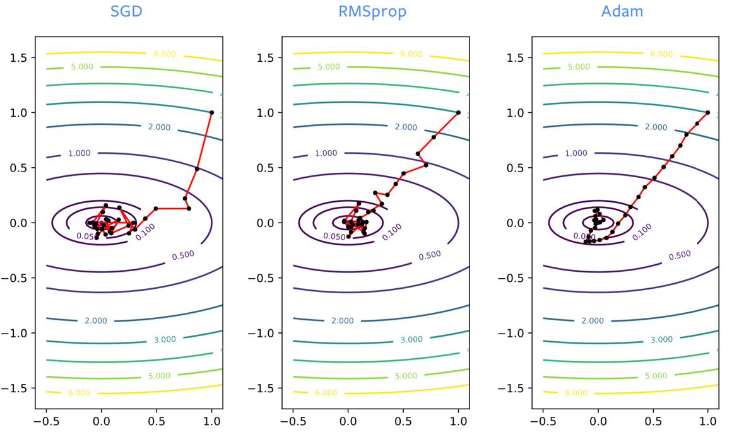
\includegraphics[width=0.7\textwidth]{figure/sgrmspropadam.png}
    \caption{Grafico che mette in luce le differenze nella convergenza fra lo SGD, la RMSprop e Adam}
    \label{fig:diffAdamSGDRMSprop}
\end{figure}

\subsection{Limitazioni di Adam}
Ovviamente Adam non è perfetto, in fatti incorre in alcune limitazioni:

\begin{itemize}
    \item\textbf{Sovra-adattamento ai dati rumorosi}: Adam si adatta velocemente, ma può reagire troppo a gradienti rumorosi, riducendo la capacità del modello di generalizzare bene;
    \item \textbf{Decay inefficace del peso}: Adam non fa un vero weight decay come la discesa del gradiente classica. Nel SGD viene incluso il parametro di regolarizzazione, questa cosa viene effettuata in Adam, nel learning rate adattivo, dunque è meno efficace;
    \item\textbf{Rallentata convergenza finale}:Adam spesso converge rapidamente all'inizio, ma poi rallenta molto nel trovare il minimo ottimale. Questo poiché i learning rate adattivi riducono troppo la velocità di aggiornamento nelle fasi finali.
\end{itemize}

\subsection{AdamW}
Per risolvere il problema del weight decay inefficace, è stato introdotto \textbf{AdamW}, dove la penalizzazione viene separata dall’aggiornamento di Adam.

\begin{equation}
        \theta_{t+1} = \theta_t - \frac{\eta}{\sqrt{\hat{v_t}}+\epsilon}\hat{m_t}\,-\,\eta\lambda \theta_t
\end{equation}

\section{Lion}
Sebbene Adam sia l'ottimizzatore più utilizzato dalla comunità scientifica, esso non è il migliore, basti pensare che nel Febbraio del 2023, è stato proposto un ottimizzatore completamente diverso da quelli precedenti, questo perché era stato proposto da un Agente di Intelligenza Artificiale. La forza di farlo fare a un calcolatore, e che le formule vennerò convertite naturalmente in linee di codice, e questa cosa ci permetteva automaticamente di calcolarne il costo computazionale, avendo preso in analisi le operazioni atomiche. E per rendere più compatto il codice l'agente ha introdotto una funzione che è esattamente quella presente in tutti gli ottimizzatori che abbiamo visto fin'ora, ossia quella di interpolazione, in modo tale da poterla inserire all'interno di varie sequenze di codice. Questo algoritmo non fa altro che prendere in analisi vari algoritmi migliorati nei vari cicli di aggiornaemnto e ne fa una sorta di torneo, combinando i migliori, generandone dei figli i quali prendono le parti migliori dei genitori, per raffinare sempre più, esattamente come le manipolazioni geniche.

\begin{python}[frame=trBL]
    def train(weight, gradient, momentum, lr):
        update = interp(gradient, momentum, (*@$\beta_1$@*))
        update = sign(update)
        momentum = interp(gradient, momentum, (*@$\beta_2$@*))
        weight_decay = weight * (*@$\lambda$@*)
        update = update + weight_decay
        update = update * lr
    return update, momentum
\end{python}

\section{Gradiente e Curvatura}
Se scegliamo una direzione in cui muoverci e continuiamo ad andare in quella direzione, di quanto diminuisce l'errore prima di ricominciare a salire? Questa è una domanda lecita che possiamo porci nel momento in cui calcoliamo il gradiente, solitamente noi assumiamo che la curvatura si acostante, cioè che si tratti duna superficie di errore quadratica, assumiamo nella nostra analisi che l'entità del gradiente diminuisca man mano che ci spostiamo verso il basso, la riduzione massima dell'errore dipende dal rapporto fra il gradiente e la curvatura, e una buona direzione nella quale è efficiente muoversi è quella con un elevato rapporto fra gradiente e curvatura, come possiamo trovare la giusta curvatura è la domanda spontanea che ci verrebbe da chiederci.

\section{Metodo di Newton}
Il Metodo di Newton si trova come soluziona a questa domanda, infatti esso integra sia la curvatura che il gradiente moltiplicando la matrice Hessiana con il gradiente. Prima di andare nel dettaglio con il metodo di Newton, ricordiamo un paio di concetti.

\subsubsection{Gradiente}
Sia $f:\mathbb{R}^n \rightarrow \mathbb{R}$ un campo scalare. Il gradiente $\nabla f:\mathbb{R}^n \rightarrow \mathbb{R}^n$ è un vettore tale che $(\nabla f)_i = \frac{\partial f}{\partial x_i}$. Poiché ogni punto nel dominio di $f$ è mappato in un vettore, allora $\nabla f$ è uno spazio vettore.

\subsubsection{Jacobian}
Sia $\mathbf{F}:\mathbb{R}^n \rightarrow \mathbb{R}^m$ è un campo vettoriale. Allora il Jacobiano può essere considerato come il campo vettoriale delle detivate. Considerando ogni componente di $\mathbf{F}$ come una singola funzione, il Jacobiano pertanto è una matrice la quale i-esima riga è il gradiente dell'i-esima componente di $\mathbf{F}$, dunque se il Jacobiano è $J$ allora:
\begin{equation}
    J_{i,j} = \frac{\partial F_i}{\partial x_j}
\end{equation}

\subsubsection{Hessiano}
Essa è la matrice delle derivate seconde parziali di ogni combinazione di elementi:
\begin{equation}
H_{ij} = \frac{\partial^2 J}{\partial x_i \partial x_j}
\end{equation}
\begin{itemize}
    \item Le \textbf{componenti diagonali} indicano la curvatura lungo un singolo asse, e coincidono con la derivata seconda;
    \item Gli \textbf{elementi fuori diagonale} descrivono le interazioni tra i pesi.
\end{itemize}
Ogni elemento nella matrice Hessiana specifica come il gradiente si modifica in una direzione, nel momento in cui ci muoviamo in un'altra direzione diversa da quella del gradiente.

Il metodo di Newton infatti introduce tramite l'utilizzo dell'inversione della matrice Hessiana la seguente relazione:

\begin{equation}
    \Delta w = -\epsilon H(w)^{-1}\frac{d E}{d w}
\end{equation}

Tuttavia questo è problematico poiché calcolare una matrice inversa oltre ad essere computazionalmente elevato, non sempre è possibile.

\subsection{Metodi Alternativi per Gestire l'Hessiano}
Poiché calcolare e invertire \( H \) è difficile, si usano approcci approssimati, per esempio quello proposto dal \textbf{Metodo Hessian-Free}, che è volto ad approssimare \( H \) e usare il metodo del gradiente coniugato per minimizzare l'errore.

\section{Gradiente Coniugato}
Il metodo del gradiente coniugato è un'alternativa al metodo di Newton per trovare il minimo di una funzione di costo senza dover invertire l'Hessiano. 
\begin{enumerate}
    \item Si sceglie una direzione iniziale basata sul gradiente;
    \item Si aggiorna il peso minimizzando lungo quella direzione;
    \item Si calcola una nuova direzione che sia coniugata alla precedente (ovvero, perpendicolare);
    \item Si ripete fino alla convergenza.
\end{enumerate}

La grandezza di questo metodo e che dopo \( N \) passi in uno spazio \( N \)-dimensionale, garantisce il minimo su una superficie quadratica, evitando inoltre oscillazioni e velocizzando la convergenza rispetto alla discesa del gradiente standard, ma soprattuto ci permette di non calcolare esplicitamente l'inversa della matrice Hessiana.

\chapter{Normalization Layers}
La normalizzazione è una tecnica cruciale nell’addestramento di reti neurali profonde. Essa viene introdotta per migliorare l’ottimizzazione e stabilizzare l'apprendimento. In particolare, si fa riferimento alla \textbf{Batch Normalization (BN)} come metodo per affrontare problemi legati al cosiddetto \textit{internal covariate shift}.

\section{Covariate Shift}
Il \textbf{Covariate Shift} rappresenta un cambiamento nella distribuzione degli input tra il training e il test. Nelle CNN \textit{(Convolutional Neural Network)} (che vedremo nel capitolo successivo), i cambiamenti nei pesi degli strati inferiori modificano la distribuzione degli input per gli strati successivi, rallentandone pertanto l'addestramento. Questo fenomeno è noto come \textit{internal covariate shift}, vi è un vero e proprio problema, legato al fatto che ci si deve continuamente adattare a nuove distribuzioni, e questa cosa inevitabilmente non farà che rallentarne la convergenza.

\subsection{Problemi di Ottimizzazione}
La BN normalizza gli input degli strati intermedi, imitando un \textit{whitening} (decorrelazione con media zero e varianza unitaria). 
Questo processo è simile alla normalizzazione iniziale degli input delle reti, ma applicato a ogni batch durante l’addestramento.

\subsection{Perché il metodo classico non funziona}
Un approccio classico, ossia allenare una rete e successivamente effettuare la normalizzazione, porta a fallire. Questo poiché la normalizzazione effettuata post hoc, non fa altro che rompere il flusso del gradiente portando a bias esplosivi. La disconnessione fra ottimizzazione e normalizzazione causa dei problemi, per esempio il gradinete non tiene contro dell'effetto della normalizzazione. Pertanto una soluzione proposta è quella di inserire un layer di normalizzazione (Figura~\ref{fig:bn-layer}) all'interno del modello, in questo modo il gradiente lo "vede" e può essere in grado di correggere i parametri della rete in maniera coerente.
\begin{figure}
    \centering
    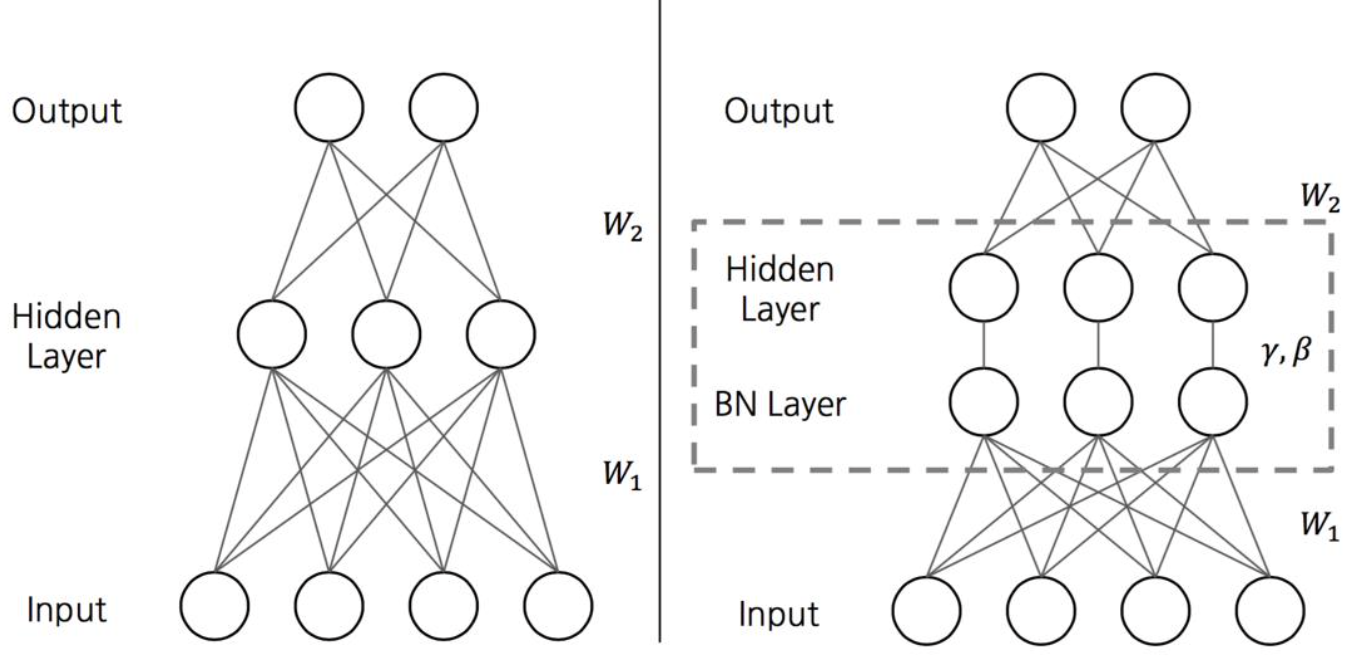
\includegraphics[width=0.85\linewidth]{figure/BNlayer.png}
    \caption{Inserimento di un layer utilizzando la Batch Normalization}
    \label{fig:bn-layer}
\end{figure}
\begin{quote}
“Il layer BN può imparare anche l’identità, rendendo reversibile la normalizzazione se necessario.”
\end{quote}

Analiziamo passo passo, quali sono i passaggi effettuati per giungere a ciò che ottimizza al meglio la Normalizzazione:
\begin{itemize}
  \item Ogni feature è normalizzata separatamente;
  \item Si usa la normalizzazione Z-score;
  \item Le stime di media e varianza vengono calcolate sul batch;
  \item Sono presenti due parametri appresi: $\gamma$ (scaling) e $\beta$ (bias), per mantenere la capacità rappresentativa.
\end{itemize}

Sia $x$ un input, $x^{(k)}$ la $k$-esima feature:

\begin{equation*}
    \mu^{(k)} = \frac{1}{m} \sum_{i=1}^m x_i^{(k)} \quad\quad \sigma^{2(k)} = \frac{1}{m} \sum_{i=1}^m (x_i^{(k)} - \mu^{(k)})^2
\end{equation*}
\begin{equation*}
    \hat{x}_i^{(k)} = \frac{x_i^{(k)} - \mu^{(k)}}{\sqrt{\sigma^{2(k)} + \epsilon}} \quad\quad y_i^{(k)} = \gamma^{(k)} \hat{x}_i^{(k)} + \beta^{(k)}
\end{equation*}

Se non ci fossero i due parametri $\beta$ e $\gamma$ la distribuzione dei valori di output, avrebbe una media nulla e una varianza unitaria e questa cosa non sarebbe utile, pertanto questi due valori non fanno altro che mantenere la forza rappresentativa della rete neurale complessiva.


\subsubsection{Perché la Batch Normalization è efficace}
\begin{itemize}
  \item Rende più stabili le distribuzioni di attivazione;
  \item Riduce l’effetto di gradienti esplosivi/vanescenti;
  \item Permette l’uso di learning rate più alti;
  \item Consente di usare attivazioni sature (e.g. sigmoid);
  \item Diminuisce la necessità di tecniche di regularizzazione;
  \item Riduce il tempo di training;
  \item Migliora la generalizzazione;
  \item Aumenta l'accuratezza.
\end{itemize}

Esistono inoltre varie tipologie di normalizzazione ed essi differiscono semplicemente per la dimensione del gruppo di campioni usati per la normalizzazione, per esempio lungo i canali, i batch presi in considerazioni o ancora la scelta di un singolo esempio.


\subsection{Conclusioni}
Sebbene la normalizzazione funzioni bene nella pratica, le ragioni della sua efficacia sono ancora controverse. In origine, la normalizzazione è stata proposta per ridurre il "Covariate Shift", ma alcuni studiosi hanno dimostrato che questa possibilità non avviene, attraverso degli esperimenti. Tuttavia, la normalizzazione è chiaramente una combinazione dei seguenti fattori:

\begin{itemize}
    \item Le reti con strati di normalizzazione sono più facili da ottimizzare, consentendo l'uso di tassi di apprendimento più elevati;
    \item La normalizzazione ha un effetto di ottimizzazione che accelera l'addestramento delle reti neurali;
    \item Le stime di media e deviazione standard, sono rumorose a causa della casualità dei campioni nel batch. Questo rumore extra si traduce in una migliore generalizzazione in alcuni casi. La normalizzazione ha un effetto di regolarizzazione;
    \item La normalizzazione riduce la sensibilità all'inizializzazione del peso.
\end{itemize}

Di conseguenza, la normalizzazione consente di essere più tranquilli: dando la possibilità di combinare quasi tutti i possibili blocchi di una rete neurale qualsiasi, avendo la possibilità di addestrarne una senza dover considerare quanto essa possa essere mal condizionata.
\chapter{Convolutional Neural Networks}

Le \textbf{Convulutional Neural Network} (CNN) sono ispirate dal funzionamento dell'organizzazione della corteccia visiva animale: così come il nostro cervello riconosce volti, forme, oggetti a partire da stimoli visivi grezzi, le CNN imparano a rilevare caratteristiche visive come bordi, texture e forme, combinandole per riconoscere oggetti più complessi. Le reti neurali che noi conosciamo bene, sono quelle completamente connesse, non adatte per elaborare delle immagini grandi. Considerando il dataset \textbf{CIFAR-10}, le immagini al suo interno sono 32x32x3 pixel, pertanto se dovessimo considerare una rete neurale completamente connessa, essa avrebbe nel suo primo layer ben 3072 pesi per un singolo neurone, il che è un numero notevolmente elevato. Nel momento in cui ci spostiamo a immagini con dimensioni più grandi (e.g 200x200x3) avrò molti più pesi per neurone (e.g 120.000). Questo è uno spreco, portando con gran probablità all'overfitting e inefficienza computazionale. La grande forza delle reti convoluzionali risiede nella ricezione degli input trattandoli come un volume tridimensionale, poiché ha unità che garantiscono ben tre dimensioni (Larghezza, Altezza e Profondità), e ogni layer permette di produrre un nuovo volume tridimensionale chiamato \textit{Activation Volume}. Ogni neurone, a differenza della \textit{fully connected} è connesso solo a una porzione locale dello spazio, chiamata \textit{receptive field}, il valore dell'estensione di questo campo di connettività è un iperparametro.
\begin{Osservazione}
    L'estensione della connettività lungo l'asse della profondità è sempre uguale alla profondità del volume di input. Dunque è necessario evidenziare questa trattazione completa della dimensione della profondità rispetto alle altre.
\end{Osservazione}

\begin{figure}
    \centering
    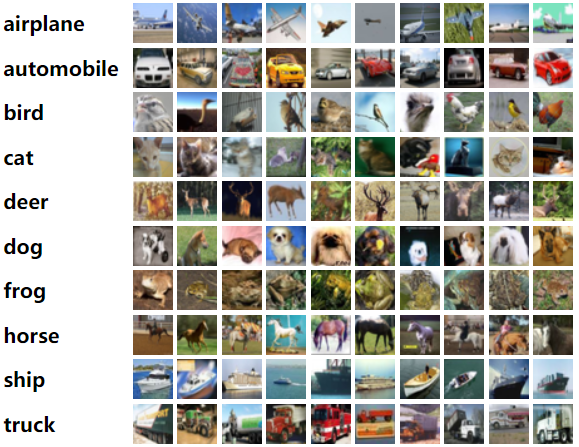
\includegraphics[width=0.40\linewidth]{figure/Cifar_dataset.png}
    \caption{Rappresentazione di una piccola parte del Cifar Dataset, contenente una delle collezioni di immagini più utilizzate nel campo del deep learning e della computer vision, per l’addestramento e la valutazione di reti neurali.}
    \label{fig:cifar_ds}
\end{figure}

\section{Analisi dell'architettura}
La rete convoluzionale è sviluppata diversamente essa è suddivisa in livelli, i quali si occupano di manipolazioni dei dati in maniere differenti e di volta in volta vi è: uno strato convoluzionale, uno strato di attivazione, uno strato di polling e uno strato completamente connesso che viene posto a conclusione della rete. Le \textbf{CNN}, applicano dei filtri, immaginabili come dei piccoli parallelepipedi aventi il compito di concentrarsi su una specifica caratteristica dell'immagine, il filtro scorre attraverso l'altezza e la larghezza della nostra immagine e apporta una convoluzione delle due, ottenendo un risultato, generando una mappa di attivazione (Figura~\ref{fig:convolution_layer}).

\begin{figure}[htbp]
    \centering
    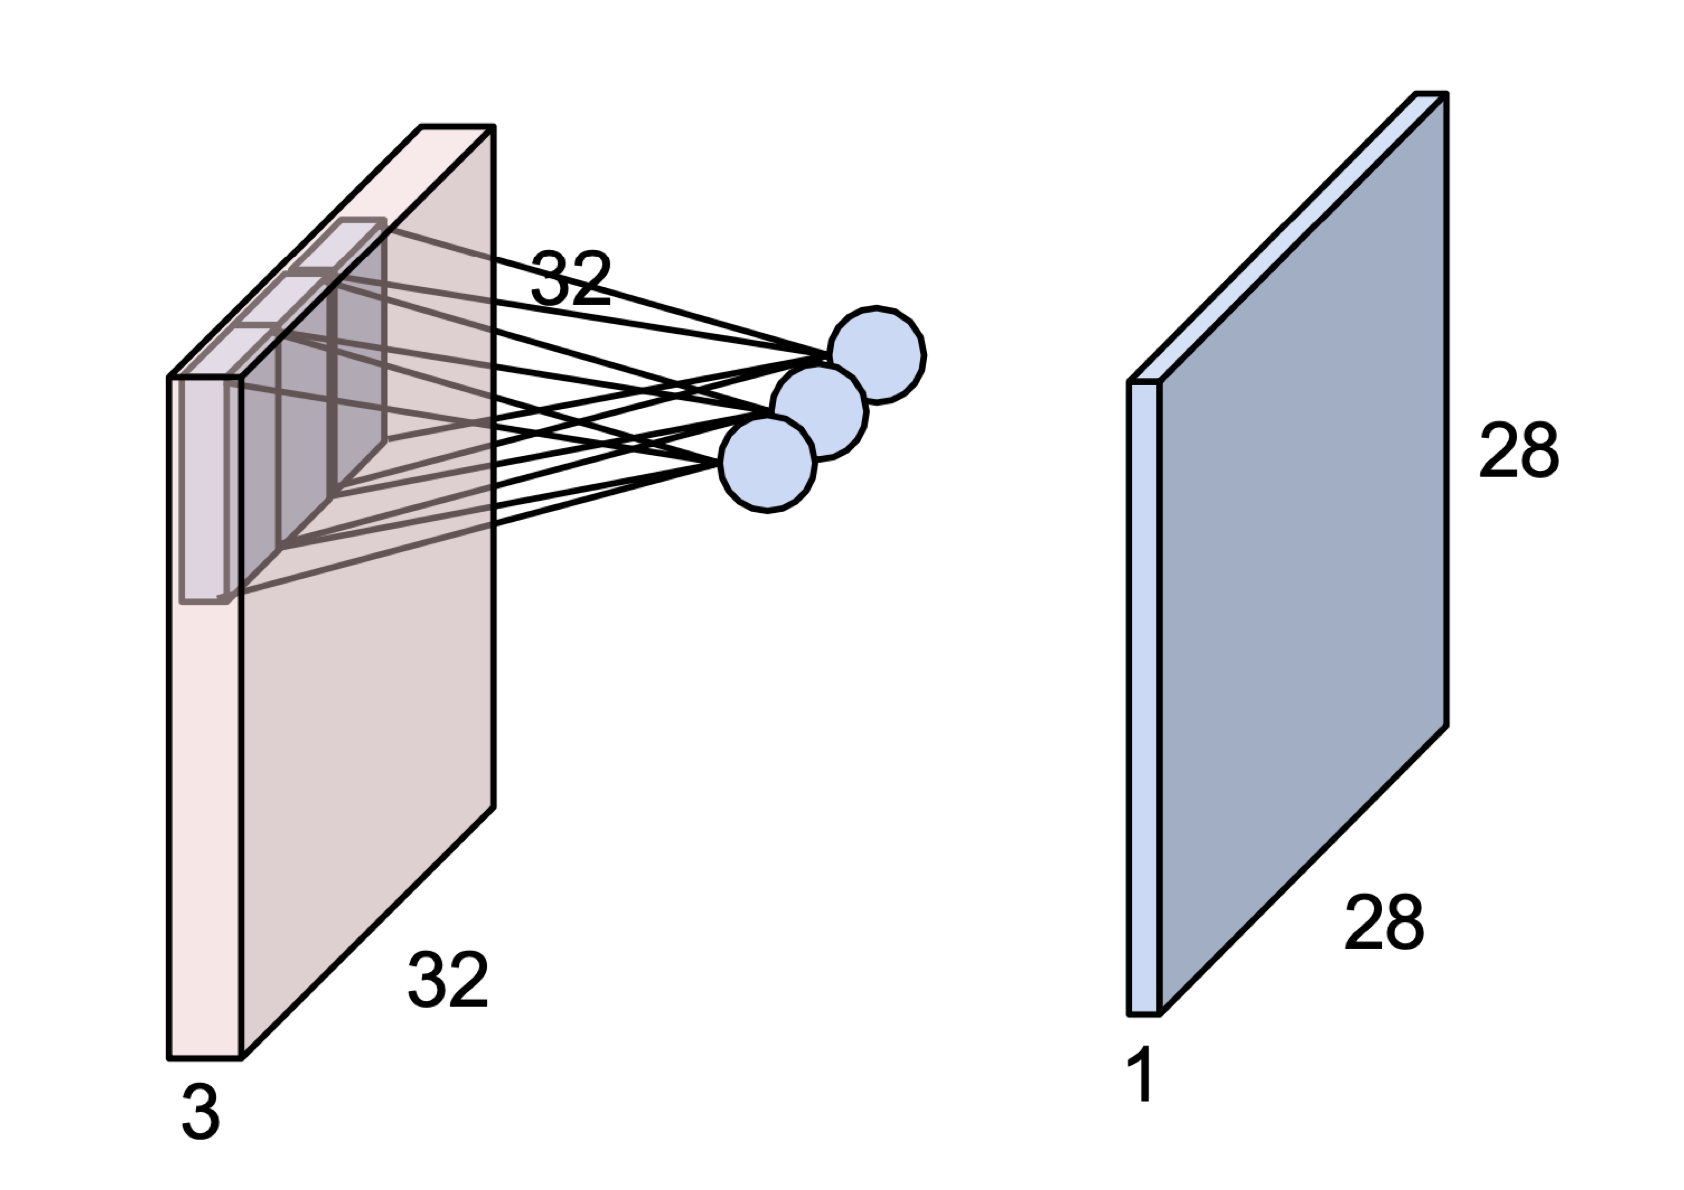
\includegraphics[width=0.55\textwidth]{figure/CNNConv.png}
    \caption{A sinistra abbiamo la rappresentazione intera dei nostri input al quale vengono applicati dei filtri, i piccolo parallelepipedi blu, i quali generano degli output, che poi una volta applicati a tutti gli input, portano alla creazione dell'activation layer, visibile in figura sulla destra.}
    \label{fig:convolution_layer}
\end{figure}

Se dovessimo limitarci esclusivamente a una singola caratteristica la rappresentazione presente in Figura~\ref{fig:convolution_layer}, ci potrebbe persino bastare. Per avere un'efficiente riconoscitore d'immagine, si utilizzano però, più filtri compattati, come se fossero un unico filtro, in modo tale da ottenere un'analisi più approfondita, ottenendo ciò che è visibile in figura~\ref{fig:convolution_layer_multifilter}. Prima di generare lo strato di attivazione vi è un'attivazione degli output ottenuti dallo strato di convoluzione, solitamente viene utilizzata la funzione \textbf{ReLU}, ma al posto di questa possiamo utilizzare una qualunque delle funzioni di attivazione presenti nel capitolo~\ref{chpt:5}.


\begin{figure}[htbp]
    \centering
    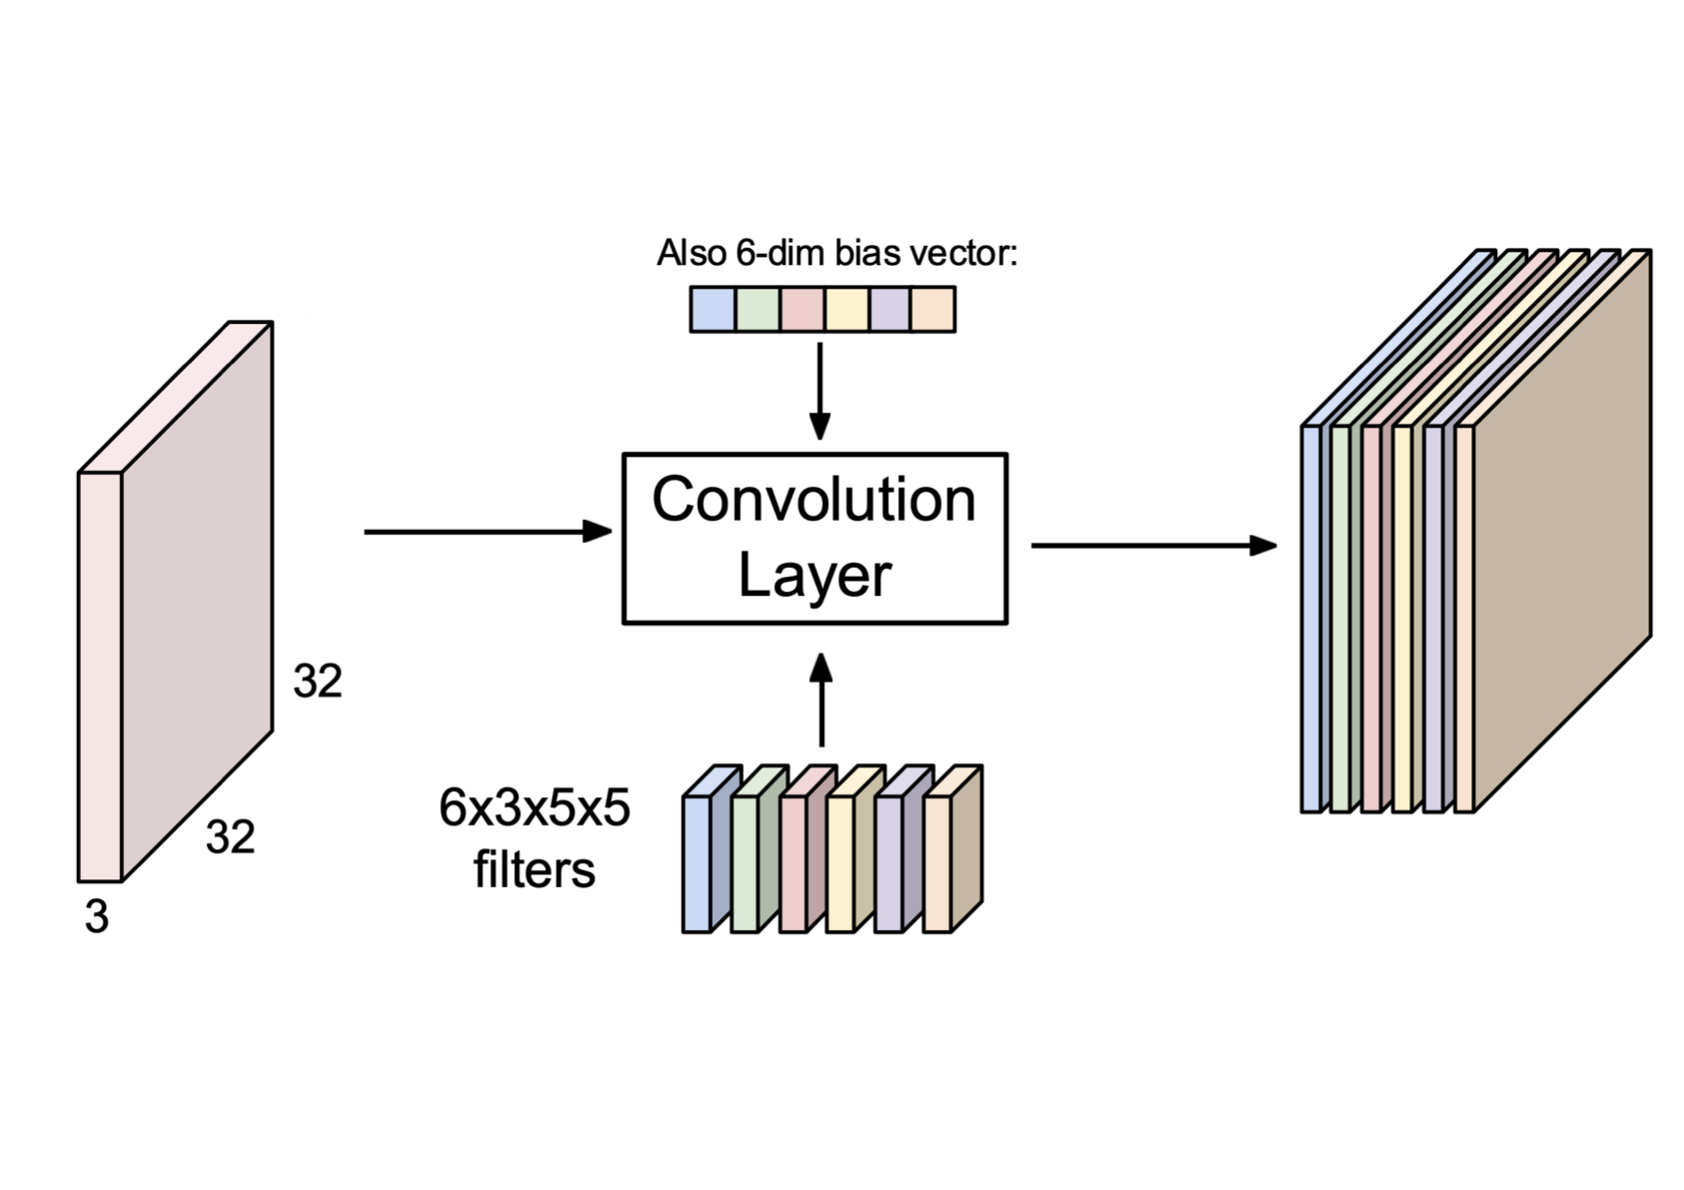
\includegraphics[width=0.85\textwidth]{figure/CNNConvolution2.png}
    \caption{Viene applicata la convoluzione con un multi filtro che permette di rilevare più feature in un'unica volta, il quale ci genera uno stack di attivazione più profondo, di quello di partenza, ma con dimensioni ridotte nelle altre dimensioni.}
    \label{fig:convolution_layer_multifilter}
\end{figure}

\section{Il filtro e le sue caratteristiche}

Quando analizziamo le reti convoluzionali, ci sono diversi layer, i quali si occupano di attività differenti. Adesso soffermiamoci su un layer, nello specifico, in una parte della costituzione di un layer, ossia il filtro. Esso può essere utilizzato in diverse maniere, per poter estrarre il layer di attivazione, la decisione della dimensionalità del filtro non è effettuata a caso, ma deve essere opportunatamente scelta in base alla dimensione dell'input layer. Una caratteristica del filtro molto importante da considerare, è il passo (stride) con cui scorre al di sopra del nostro input layer, ossia di quanto si discosta una volta che ho applicato il filtro la prima volta prima di essere applicato una seconda (Figura~\ref{fig:filter_stride}). 
\begin{figure}
    \centering
    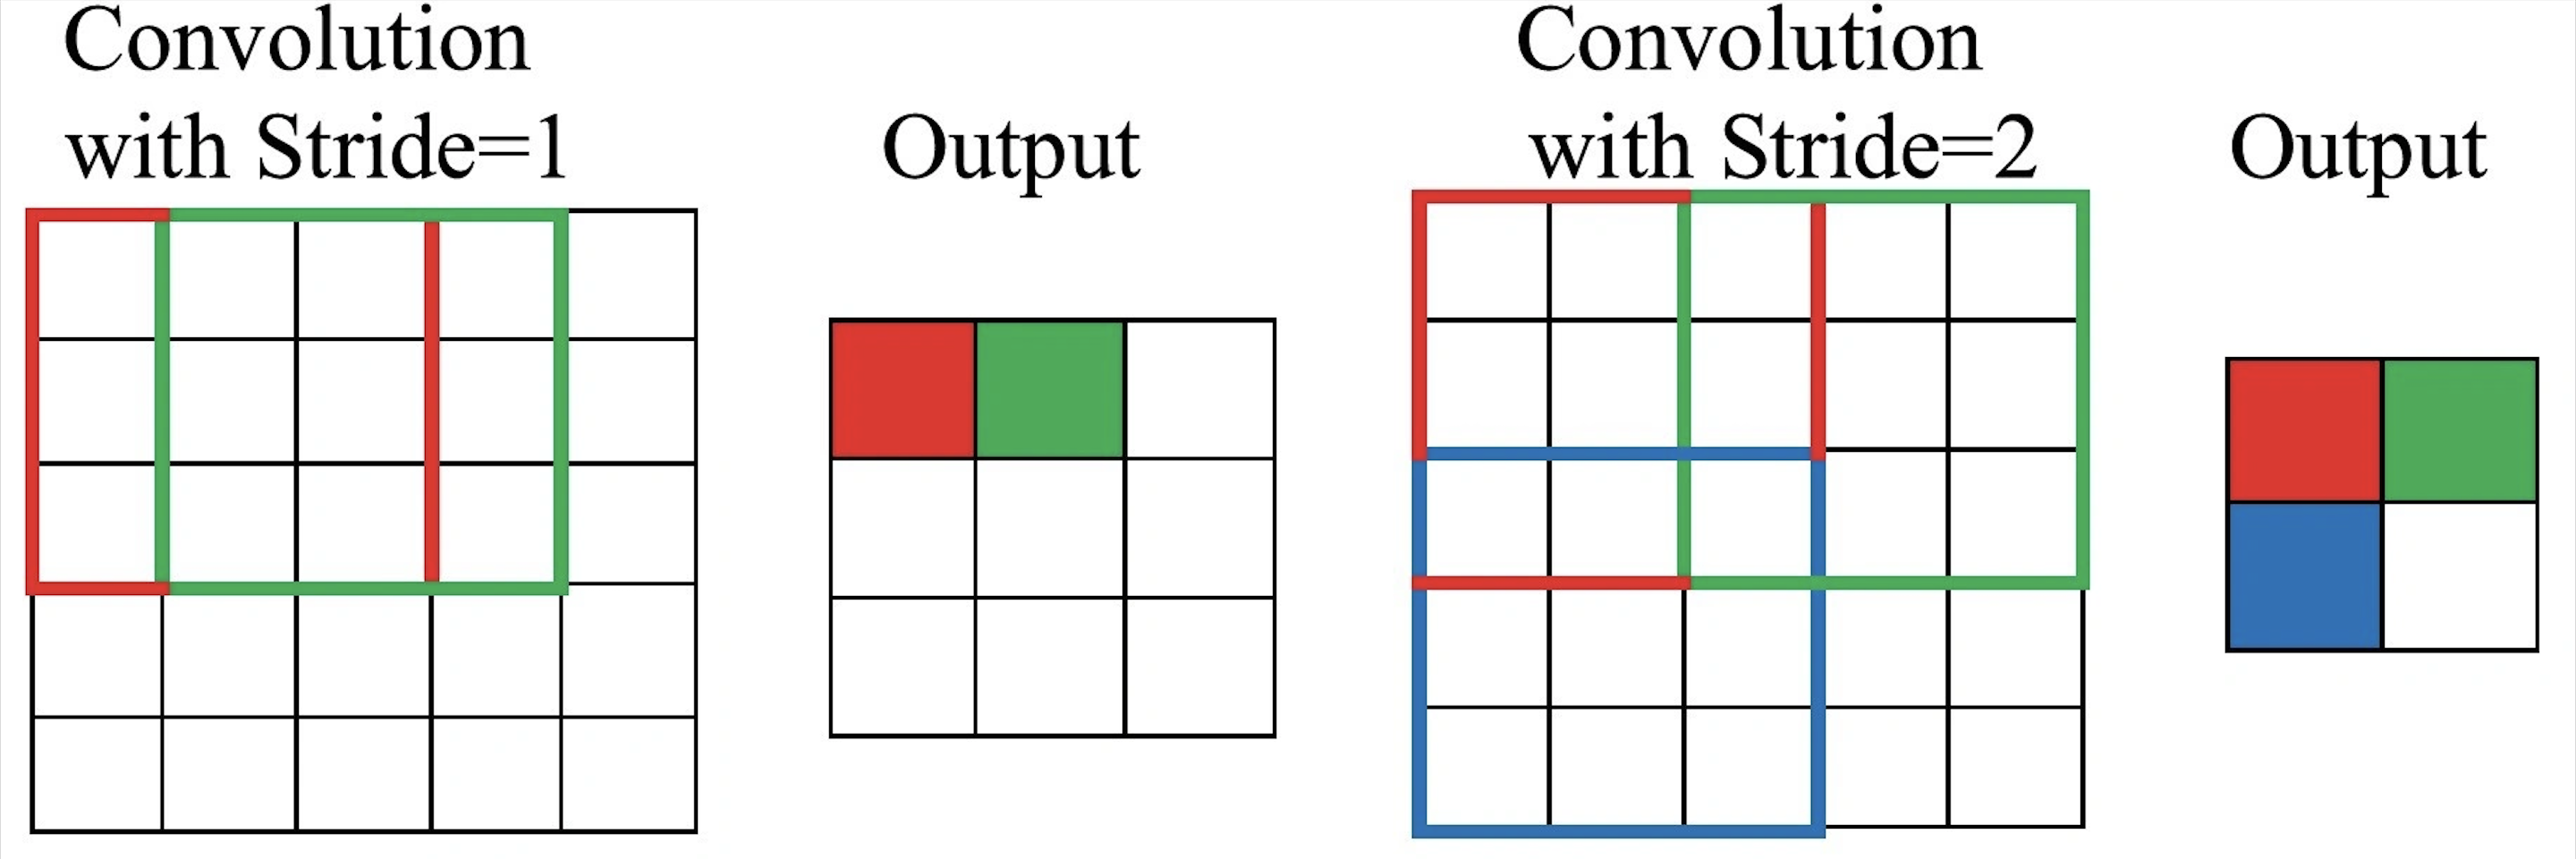
\includegraphics[width=0.90\textwidth]{figure/Filtering_stride.png}
    \caption{Applicazione di un filtro a uno stesso input layer, con a sinistra uno passo di uno, mentre a destra con un passo di due, generando a un output layer di dimensionalità differente.}
    \label{fig:filter_stride}
\end{figure}

Per calcolare invece la dimensione dell'output, si utilizza una semplice equazione, la quale tiene conto della dimensione dell'input ($N$), la dimensione del filtro ($F$) e la dimensione dello stride utilizzato ($S$).

\begin{equation}
    Output = \frac{N-F}{S} + 1
\end{equation}

Nella pratica invece, viene aggiunto un padding intorno al nostro input layer, prima ancora che venga applicato il filtro con il suo stride. Questo avviene perché, nel momento in cui andiamo ad applicare il filtro, privato di questo padding, riceveremo un rimpicciolimento dell'immagine, che in realtà è il nostro scopo reale, tuttavia dopo numerosi strati l'immagine giunge a delle dimensioni molto ridotte, pertanto non risulta più una riduzione efficiente. Se non applicassimo il padding, i pixel posti ai bordi verrebbero utilizzati molto meno nel calcolo della convoluzione, invece con il padding, tutti i pixel partecipano con la stessa frequenza e importanza a ogni convoluzione. Non utilizzare il padding inoltre, porterebbe a una perdita d'informazione, poiché viene tagliata la parte più esterna dell'immagine, mentre utilizzandolo si conserverebbe più contesto visivo. L'equazione della dimensione dell'otuput pertanto si modifica nel seguente modo:

\begin{equation}
    Output = \frac{N+2P-F}{S} +1
\end{equation}

\subsection{Filtri 1x1}

I filtri 1x1 nelle reti neurali convoluzionali (CNN) possono sembrare controintuitivi, ma svolgono ruoli fondamentali nell'ottimizzazione e nella potenza espressiva delle reti. Un filtro 1x1 applica una convoluzione su ogni pixel, considerando però tutti i canali (eg. R, G, B) contemporaneamente. Non modifica la dimensione spaziale (altezza e larghezza), ma agisce sulla profondità (numero di canali). Esso può servire per:

\begin{itemize}
    \item \textbf{Riduzione della dimensionalità:} Un filtro 1×1 può ridurre il numero di canali, diminuendo così i parametri e i costi computazionali. Ad esempio, da 256 canali a 64;
    \item \textbf{Aumento della dimensionalità:} Al contrario, può aumentare i canali per arricchire la rappresentazione dei dati;
    \item \textbf{Aggiunta di non linearità:} Combinato con funzioni di attivazione (eg. ReLU), introduce non-linearità, migliorando la capacità di apprendimento della rete;
    \item \textbf{Interazione tra canali:} Permette di combinare informazioni tra diversi canali, facilitando l'apprendimento di caratteristiche complesse.
\end{itemize}


\section{Receptive Fields Estesi}

Il Receptive Field (campo recettivo) è la porzione dell’immagine originale che influenza l’attivazione di un singolo neurone in uno specifico strato. Più si va in profondità nella rete, più il campo visivo del neurone si espande: cominciando a vedere regioni più grandi dell'immagine (Figura~\ref{fig:recp_field}). Questo perché se mi muovo in un layer più profondo oltre a visualizzare alcuni neuroni, vedrò anche ciò che vedono i singoli neuroni a loro volta, e per questo espandero il mio campo recettivo, avendo una visione di insieme, sempre più espansa.
\begin{figure}
    \centering
    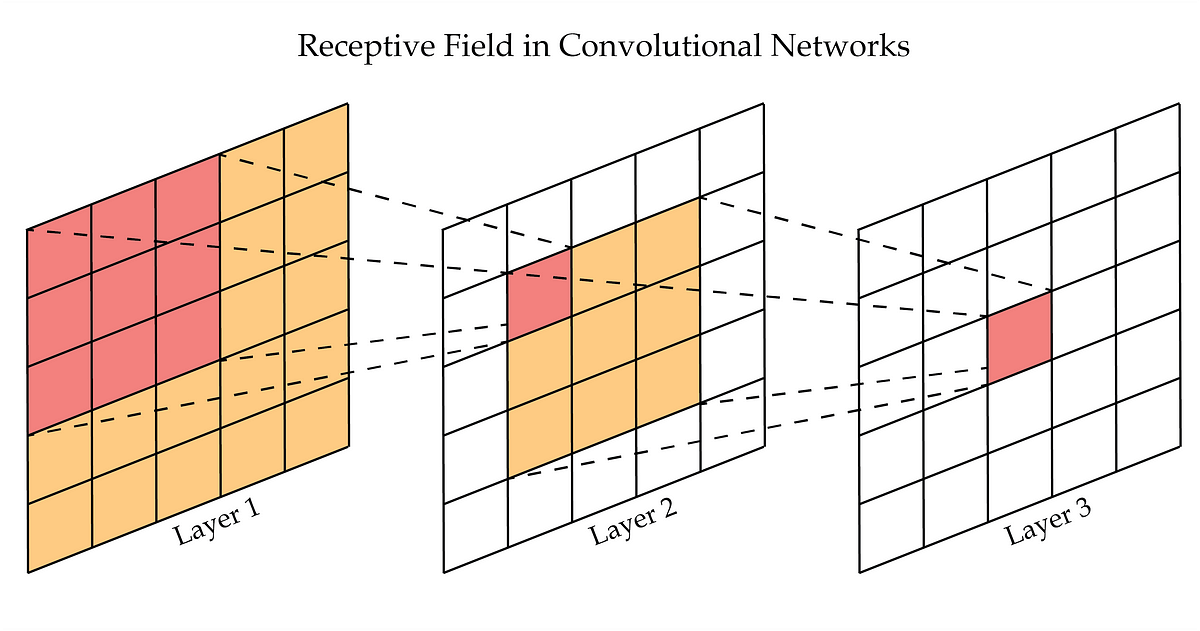
\includegraphics[width=0.75\textwidth]{figure/receptive_field.png}
    \caption{Rappresentazione del receptive field, su tre layer}
    \label{fig:recp_field}
\end{figure}
Considerando $L$ come il layer in cui ci troviamo e $K$ come il numero di dimensione del filtro, possiamo calcolare il Receptive Field ($R$), nel seguente modo:
\[
R = 1 + L \cdot (K - 1)
\]
Dunque possiamo arrivarci intuitivamente, per ottenere una visione globale dell'immagine che stiamo analizzando, avremo bisogno di numerosi layer convoluzionali.
\section{Pooling Layer}

I livelli di \textit{Pooling} sono tipicamente interposti tra strati convoluzionali all'interno delle reti neurali convoluzionali (CNN). La loro funzione principale è quella di ridurre progressivamente la dimensione spaziale delle mappe di attivazione, attraverso un processo di \textit{downsampling}. Questo consente di diminuire il numero di parametri e il carico computazionale della rete, mitigare il rischio di overfitting e favorire l’invarianza a piccole traslazioni dell’input. Le operazioni di pooling più comuni includono:
\begin{itemize}
    \item \textbf{Max Pooling:} seleziona il valore massimo all'interno di una finestra locale (kernel) sull'immagine di input;
    \item \textbf{Average Pooling:} calcola la media dei valori nella regione coperta dal kernel;
    \item \textbf{Sum Pooling:} somma tutti i valori nella regione considerata;
\end{itemize}

Attraverso il pooling si ottiene una rappresentazione più compatta delle mappe di caratteristiche, preservando le informazioni più salienti. Questo processo di sottocampionamento permette alla rete di concentrarsi sulle caratteristiche più significative, riducendo al contempo la sensibilità a piccole variazioni locali. Combinando in modo efficace strati convoluzionali e di pooling, una CNN è in grado di apprendere progressivamente rappresentazioni gerarchiche dell’input, rilevando strutture sempre più complesse come bordi, texture, oggetti o intere scene. Infine, l’output dello strato convoluzionale finale viene \textit{appiattito} in un vettore monodimensionale, che viene successivamente fornito a uno o più strati completamente connessi (\textit{fully connected}) per eseguire il compito di classificazione.

\begin{figure}[ht]
    \centering
    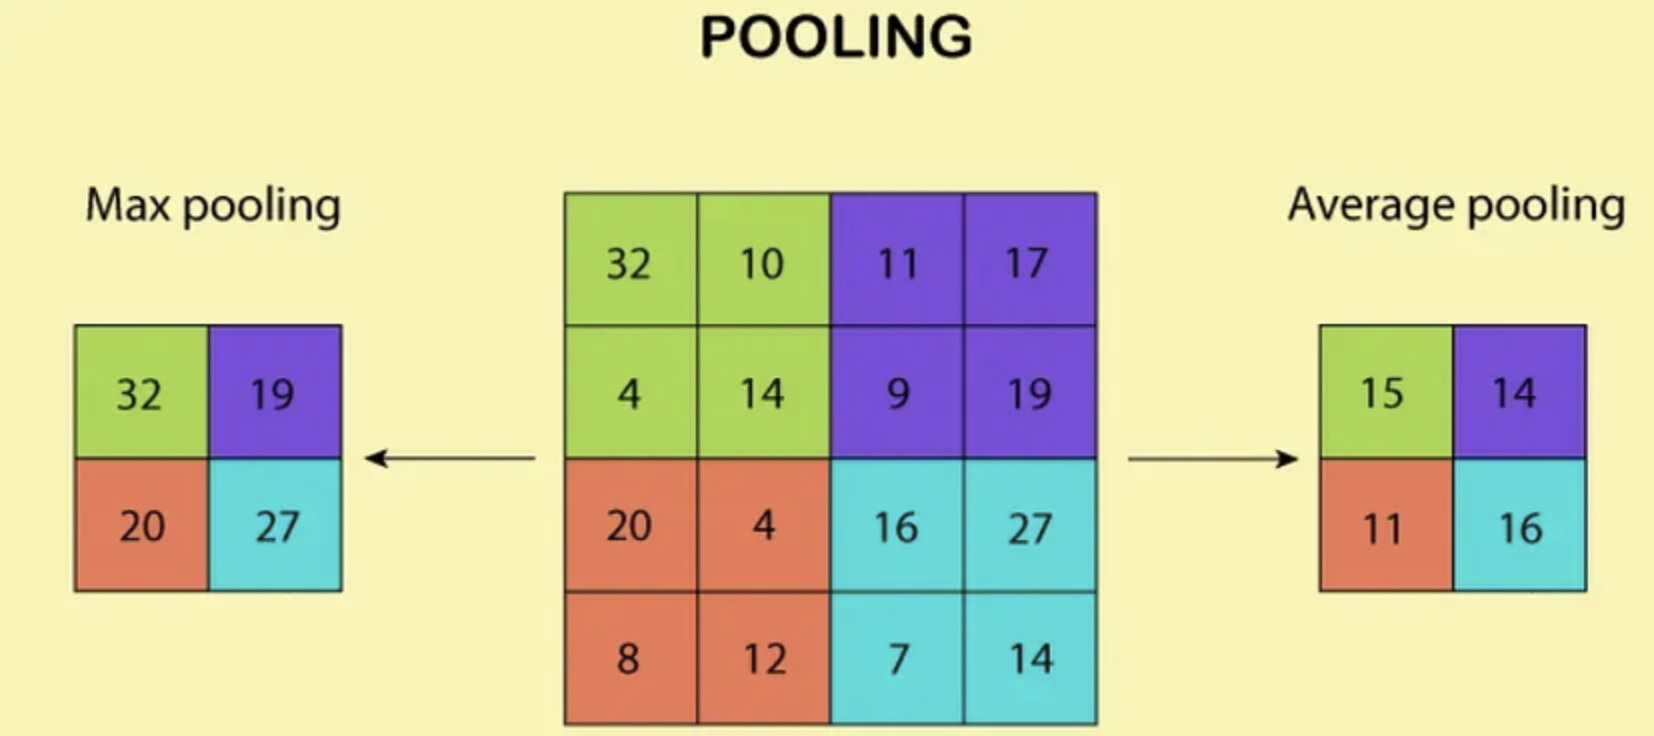
\includegraphics[width=0.55\textwidth]{figure/Pooling.png}
    \caption{Effetto del pooling applicato con kernel $2 \times 2$ e stride 2: a sinistra, il valore massimo selezionato per ciascuna finestra (Max Pooling); a destra, la media dei valori nella stessa finestra (Average Pooling).}
    \label{fig:pooling}
\end{figure}

\section{Conclusioni}

Le reti neurali convoluzionali (CNN) sfruttano in modo efficiente la struttura spaziale delle immagini attraverso tre principi fondamentali: la connettività locale, la condivisione dei pesi mediante l’impiego di filtri convoluzionali, e l’organizzazione gerarchica dei livelli. Questi elementi architetturali consentono una significativa riduzione del numero di parametri, migliorano la capacità di generalizzazione del modello e rendono la rete scalabile su immagini di grandi dimensioni. L’uso della connettività locale permette di concentrarsi su porzioni limitate dell’input, mentre la condivisione dei pesi garantisce l’invarianza traslazionale e riduce il costo computazionale. Al termine della sequenza di strati convoluzionali e di pooling, le mappe di attivazione vengono appiattite e passate a uno o più strati completamente connessi (\textit{fully connected layers}), i quali svolgono la fase finale di classificazione. Questo approccio modulare e gerarchico rende le CNN particolarmente adatte a compiti complessi di riconoscimento visivo, come dimostrato in molteplici contesti applicativi già trattati in corsi precedenti.

\begin{figure}[ht]
    \centering
    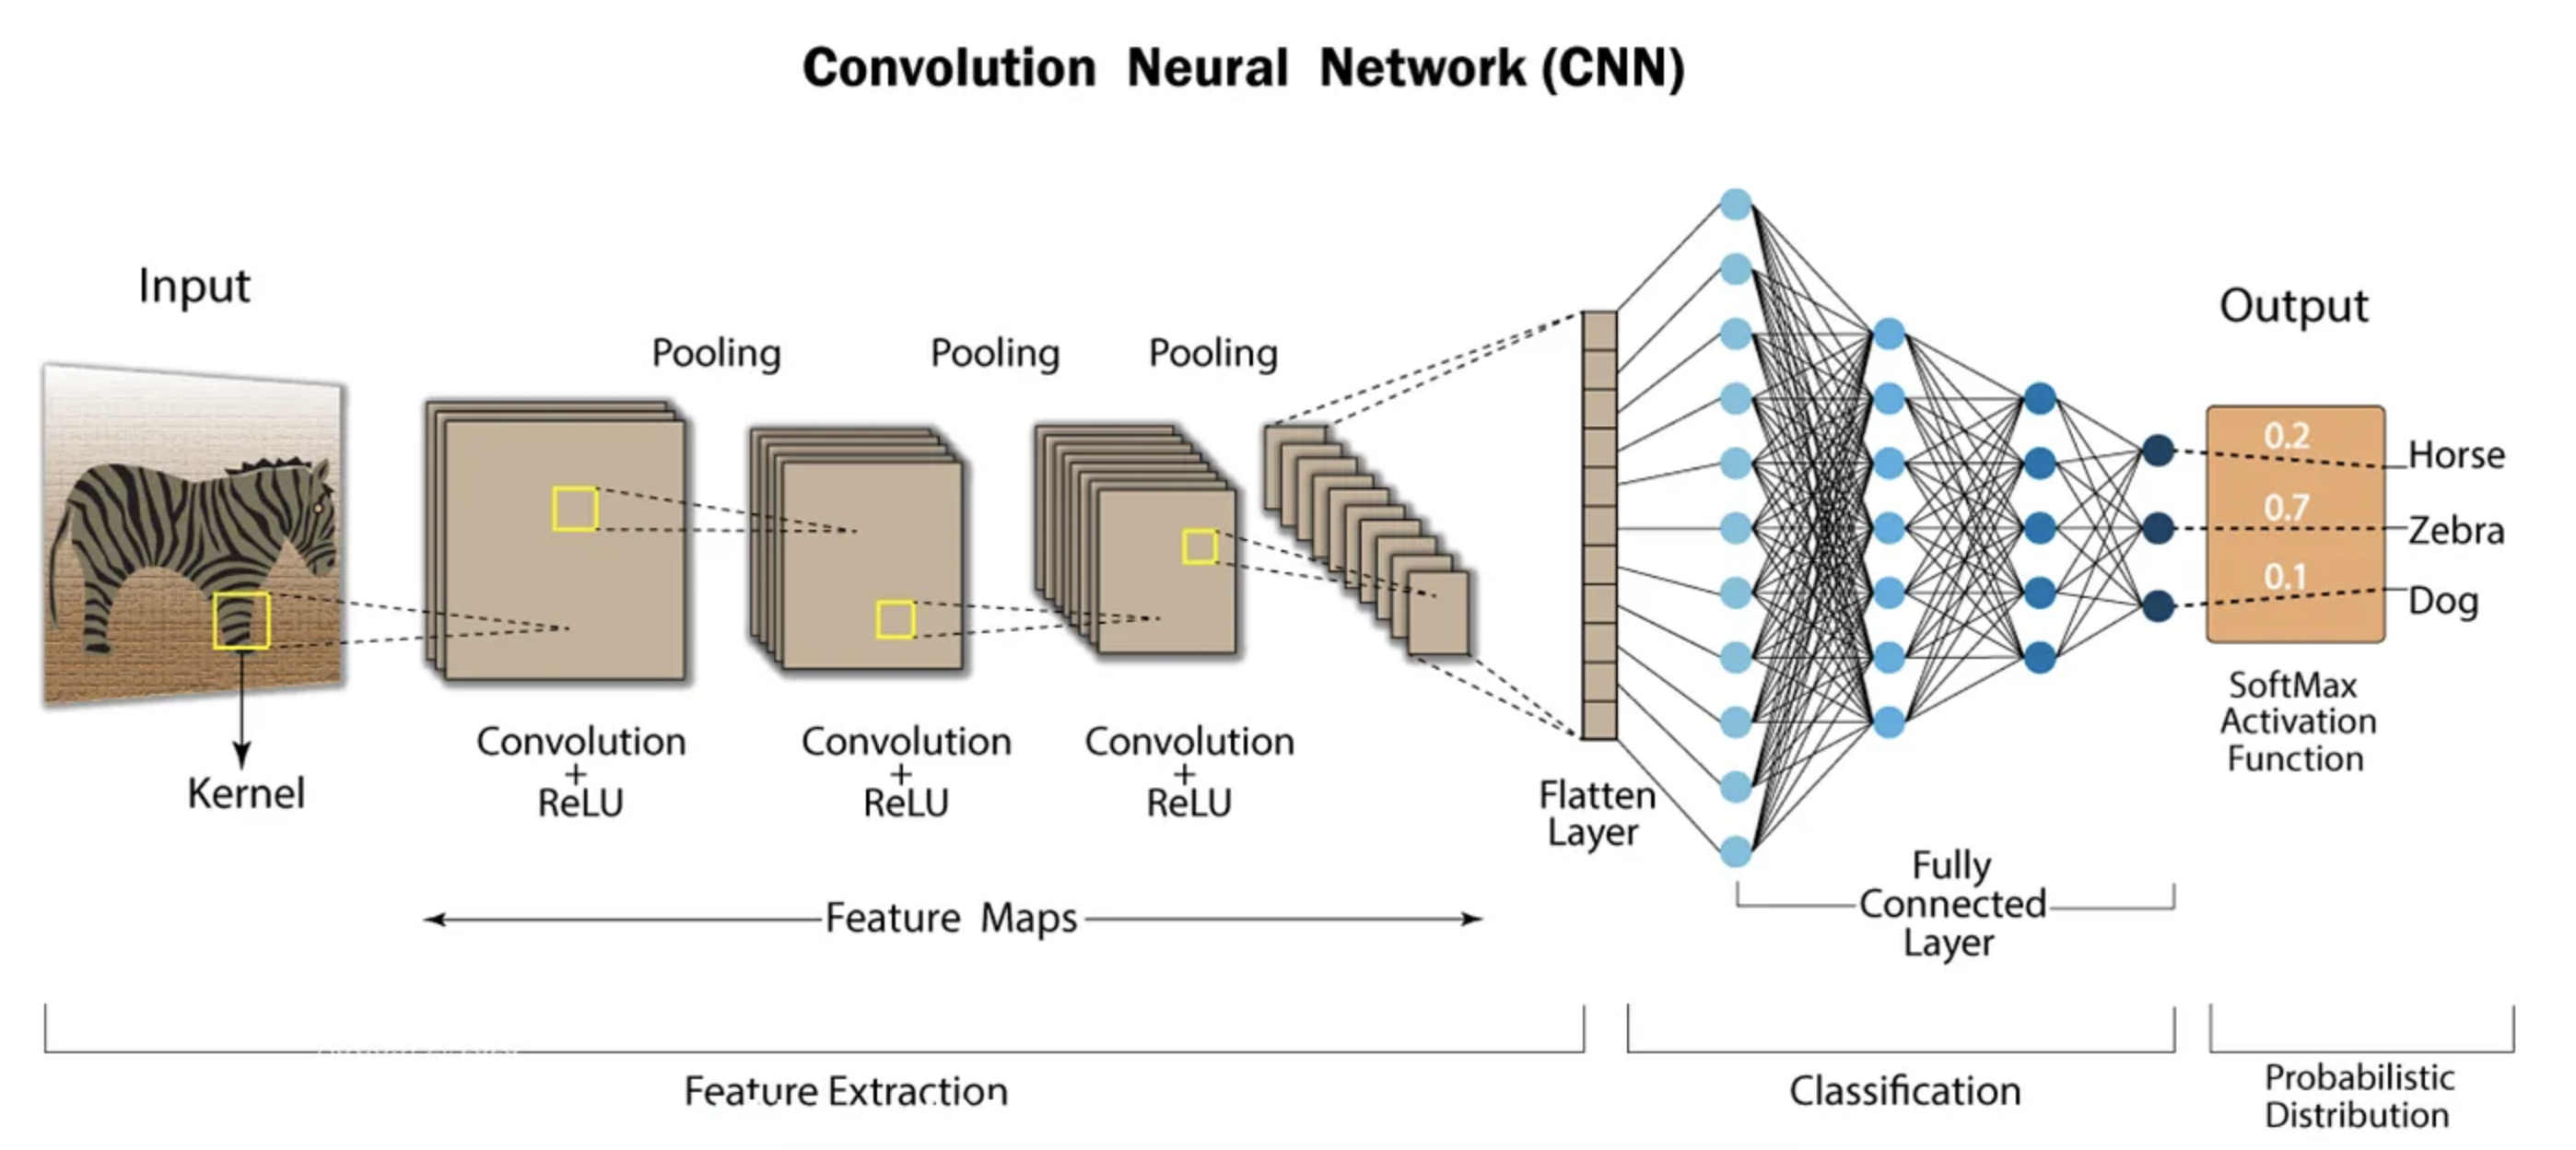
\includegraphics[width=\textwidth]{figure/ConvNN.png}
    \caption{Rappresentazione schematica di una rete neurale convoluzionale. Ogni livello svolge un’operazione distinta, contribuendo all’estrazione progressiva delle caratteristiche rilevanti dall’immagine.}
    \label{fig:ConvNN}
\end{figure}


\begin{table}[ht]
    \centering
    \caption{Confronto tra reti convoluzionali (CNN) e reti completamente connesse (Dense)}
    \label{tab:cnn_vs_dense}
    \begin{adjustbox}{width=\textwidth}
    \begin{tabular}{p{4.5cm}|p{4.5cm}|p{4.5cm}}
        \hline
        \textbf{Caratteristica} & \textbf{Reti Dense} & \textbf{Reti Convoluzionali} \\
        \hline
        Architettura & Ogni neurone connesso a tutti gli altri & Connettività locale tra neuroni \\
        \hline
        Numero di parametri & Elevato, cresce rapidamente con la dimensione dell’input & Ridotto grazie alla condivisione dei pesi \\
        \hline
        Efficienza computazionale & Bassa per immagini ad alta risoluzione & Alta, grazie all’uso di kernel \\
        \hline
        Invarianza traslazionale & Non intrinseca & Intrinseca grazie ai filtri convoluzionali \\
        \hline
        Adattabilità alle immagini & Limitata, richiede preprocessing intenso & Alta, adatte all’elaborazione visiva diretta \\
        \hline
        Capacità di generalizzazione & Tende a overfittare su dataset piccoli & Migliore grazie al minor numero di parametri \\
        \hline
    \end{tabular}
    \end{adjustbox}
\end{table}

\chapter{Recurrent Neural Networks}

Le \textbf{Recurrent Neural Networks} (RNN) costituiscono una classe di architetture neurali progettate specificamente per l’elaborazione di dati sequenziali, come segnali temporali, testi o serie temporali. A differenza delle reti neurali \textit{feed-forward}, che elaborano gli input in maniera indipendente, le RNN sono dotate di una memoria interna che evolve dinamicamente nel tempo. Questa memoria consente al modello di conservare informazioni riguardanti gli stati precedenti della sequenza, rendendo possibile la modellazione delle dipendenze temporali o contestuali tra gli elementi della serie. Tale proprietà è fondamentale in applicazioni dove il significato di un dato dipende fortemente dal contesto, come nella traduzione automatica, nel riconoscimento vocale o nella generazione di testo. L'introduzione dello stato ricorrente permette dunque di superare i limiti delle architetture tradizionali, che trattavano ogni istante temporale come isolato, senza tenere conto delle relazioni tra eventi consecutivi.

\section{Predizione sequenziale}

Consideriamo il caso di un'immagine che mostra una sfera in una determinata posizione. Una domanda naturale che potremmo porci è: \textit{quale sarà il prossimo movimento della sfera? In quale direzione si sposterà?} L'obiettivo, dunque, è predire il movimento futuro della sfera basandosi su una sequenza di osservazioni precedenti. Questo tipo di compito si adatta perfettamente all'architettura delle \textbf{Recurrent Neural Networks} (RNN), in quanto tali modelli sono in grado di mantenere uno stato interno che evolve nel tempo e che cattura le dipendenze temporali tra gli input. Nello specifico, la sfera e il suo movimento possono essere rappresentati come una sequenza temporale, dove lo stato corrente è influenzato dagli stati precedenti. Un altro esempio emblematico è il testo: possiamo infatti interpretare una frase come una sequenza di parole, dove ciascuna parola dipende in misura più o meno forte da quelle che la precedono. In tale contesto, le RNN risultano particolarmente efficaci, poiché riescono a conservare informazioni contestuali pregresse utili sia alla comprensione che alla generazione del linguaggio.

\section{Predizione della parola successiva}

Consideriamo ora la frase: \textit{This morning I took my cat for a walk}. L'obiettivo è prevedere l'ultima parola conoscendo le precedenti. Questo problema è tipico nei modelli linguistici, dove si cerca di stimare la distribuzione di probabilità condizionata per una parola data una sequenza di parole precedenti. Le RNN si rivelano utili in questo contesto, poiché riescono ad utilizzare l'intero contesto passato per calcolare la probabilità della parola successiva. Tuttavia, anche queste reti incontrano difficoltà nel trattare contesti molto lunghi, a causa di problemi noti come la \textbf{scomparsa del gradiente}, che ostacolano l’apprendimento di dipendenze a lungo termine.

\subsection{Finestra fissa}

Una strategia alternativa consiste nell'utilizzare una \textbf{finestra temporale fissa} di parole per predire la successiva. In questo caso, solo un numero limitato di parole precedenti viene considerato come input per la previsione. Tuttavia, questa scelta comporta una perdita di contesto: se la finestra è troppo piccola, il modello rischia di ignorare informazioni fondamentali; se è troppo grande, può diventare inefficiente e soggetta a instabilità, a causa del già citato problema della scomparsa del gradiente. Nel nostro esempio, se considerassimo soltanto le due parole precedenti, sarebbe molto improbabile riuscire a predire correttamente la parola finale. L’ampliamento della finestra può sembrare una soluzione, ma deve essere bilanciato per evitare un aumento eccessivo della complessità computazionale.

\subsection{One-hot encoding}

Una rappresentazione comune delle parole è il \textbf{one-hot encoding}, dove ogni parola è codificata come un vettore binario in cui un solo elemento è attivo (cioè pari a 1), mentre tutti gli altri sono a zero. Sebbene semplice, questa rappresentazione è poco efficiente dal punto di vista semantico, poiché non cattura alcuna relazione tra parole simili. Per superare tali limitazioni si introducono i \textbf{word embeddings}, rappresentazioni dense e continue che posizionano le parole in uno spazio vettoriale tale che termini semanticamente simili risultino geometricamente vicini.

\subsection{Bag of Words}

Un ulteriore approccio è il \textbf{Bag of Words} (BoW), in cui l'intera frase viene rappresentata come un vettore che indica la presenza o assenza di ogni parola, indipendentemente dalla loro posizione. Tuttavia, tale metodo ignora completamente l’ordine delle parole, il quale è invece cruciale per la comprensione sintattica e semantica del linguaggio. Un cambiamento minimo nell’ordine delle parole può alterare radicalmente il significato di una frase. Le RNN, al contrario, preservano l’ordine sequenziale degli input e permettono di modellare strutture linguistiche complesse, grazie alla loro capacità di mantenere la memoria temporale e adattarsi a dipendenze di lungo periodo.

\begin{table}[htbp]
\centering
\footnotesize
\caption{Confronto tra approcci per la rappresentazione del testo e la predizione sequenziale.}
\begin{adjustbox}{width=\textwidth}
\begin{tabular}{l|p{3.8cm}|p{3.5cm}|p{3.5cm}}
\hline
\textbf{Metodo} & \textbf{Caratteristiche principali} & \textbf{Vantaggi} & \textbf{Svantaggi} \\
\hline
\textbf{Finestra fissa} & Considera solo $n$ parole precedenti & Computazionalmente semplice & Non gestisce dipendenze a lungo termine \\
\hline
\textbf{One-hot encoding} & Rappresentazione binaria con un solo 1 attivo & Facile da implementare & Non cattura relazioni semantiche \\
\hline
\textbf{Bag of Words (BoW)} & Rappresenta la presenza o frequenza delle parole ignorando l’ordine & Semplice e interpretabile & Perde completamente l’informazione sull’ordine \\
\hline
\textbf{Word Embeddings} & Vettori densi che catturano somiglianze semantiche & Efficienza e rappresentazione semantica & Richiede training e risorse computazionali \\
\hline
\end{tabular}
\end{adjustbox}
\label{tab:metodi_sequenziali}
\end{table}

\section{Architettura delle RNN}

Le reti neurali \textit{feedforward} elaborano gli input in un'unica direzione, dall'input all'output, senza tenere conto della sequenzialità o della dipendenza temporale dei dati. In tal modo, presuppongono che ogni input e output sia indipendente dagli altri. Questa assunzione le rende inadatte a compiti in cui il contesto o l'ordine temporale sono fondamentali (es. traduzione, modellazione linguistica, riconoscimento vocale). Le Reti Neurali Ricorrenti (RNN), invece, sono progettate per lavorare su sequenze, riconoscendo pattern temporali grazie alla capacità di mantenere una \textit{memoria} implicita dello stato precedente della rete. In altre parole, una RNN può sfruttare informazioni precedenti per influenzare le previsioni successive, rendendola adatta a compiti dove la storia è rilevante.
\begin{figure}
\centering
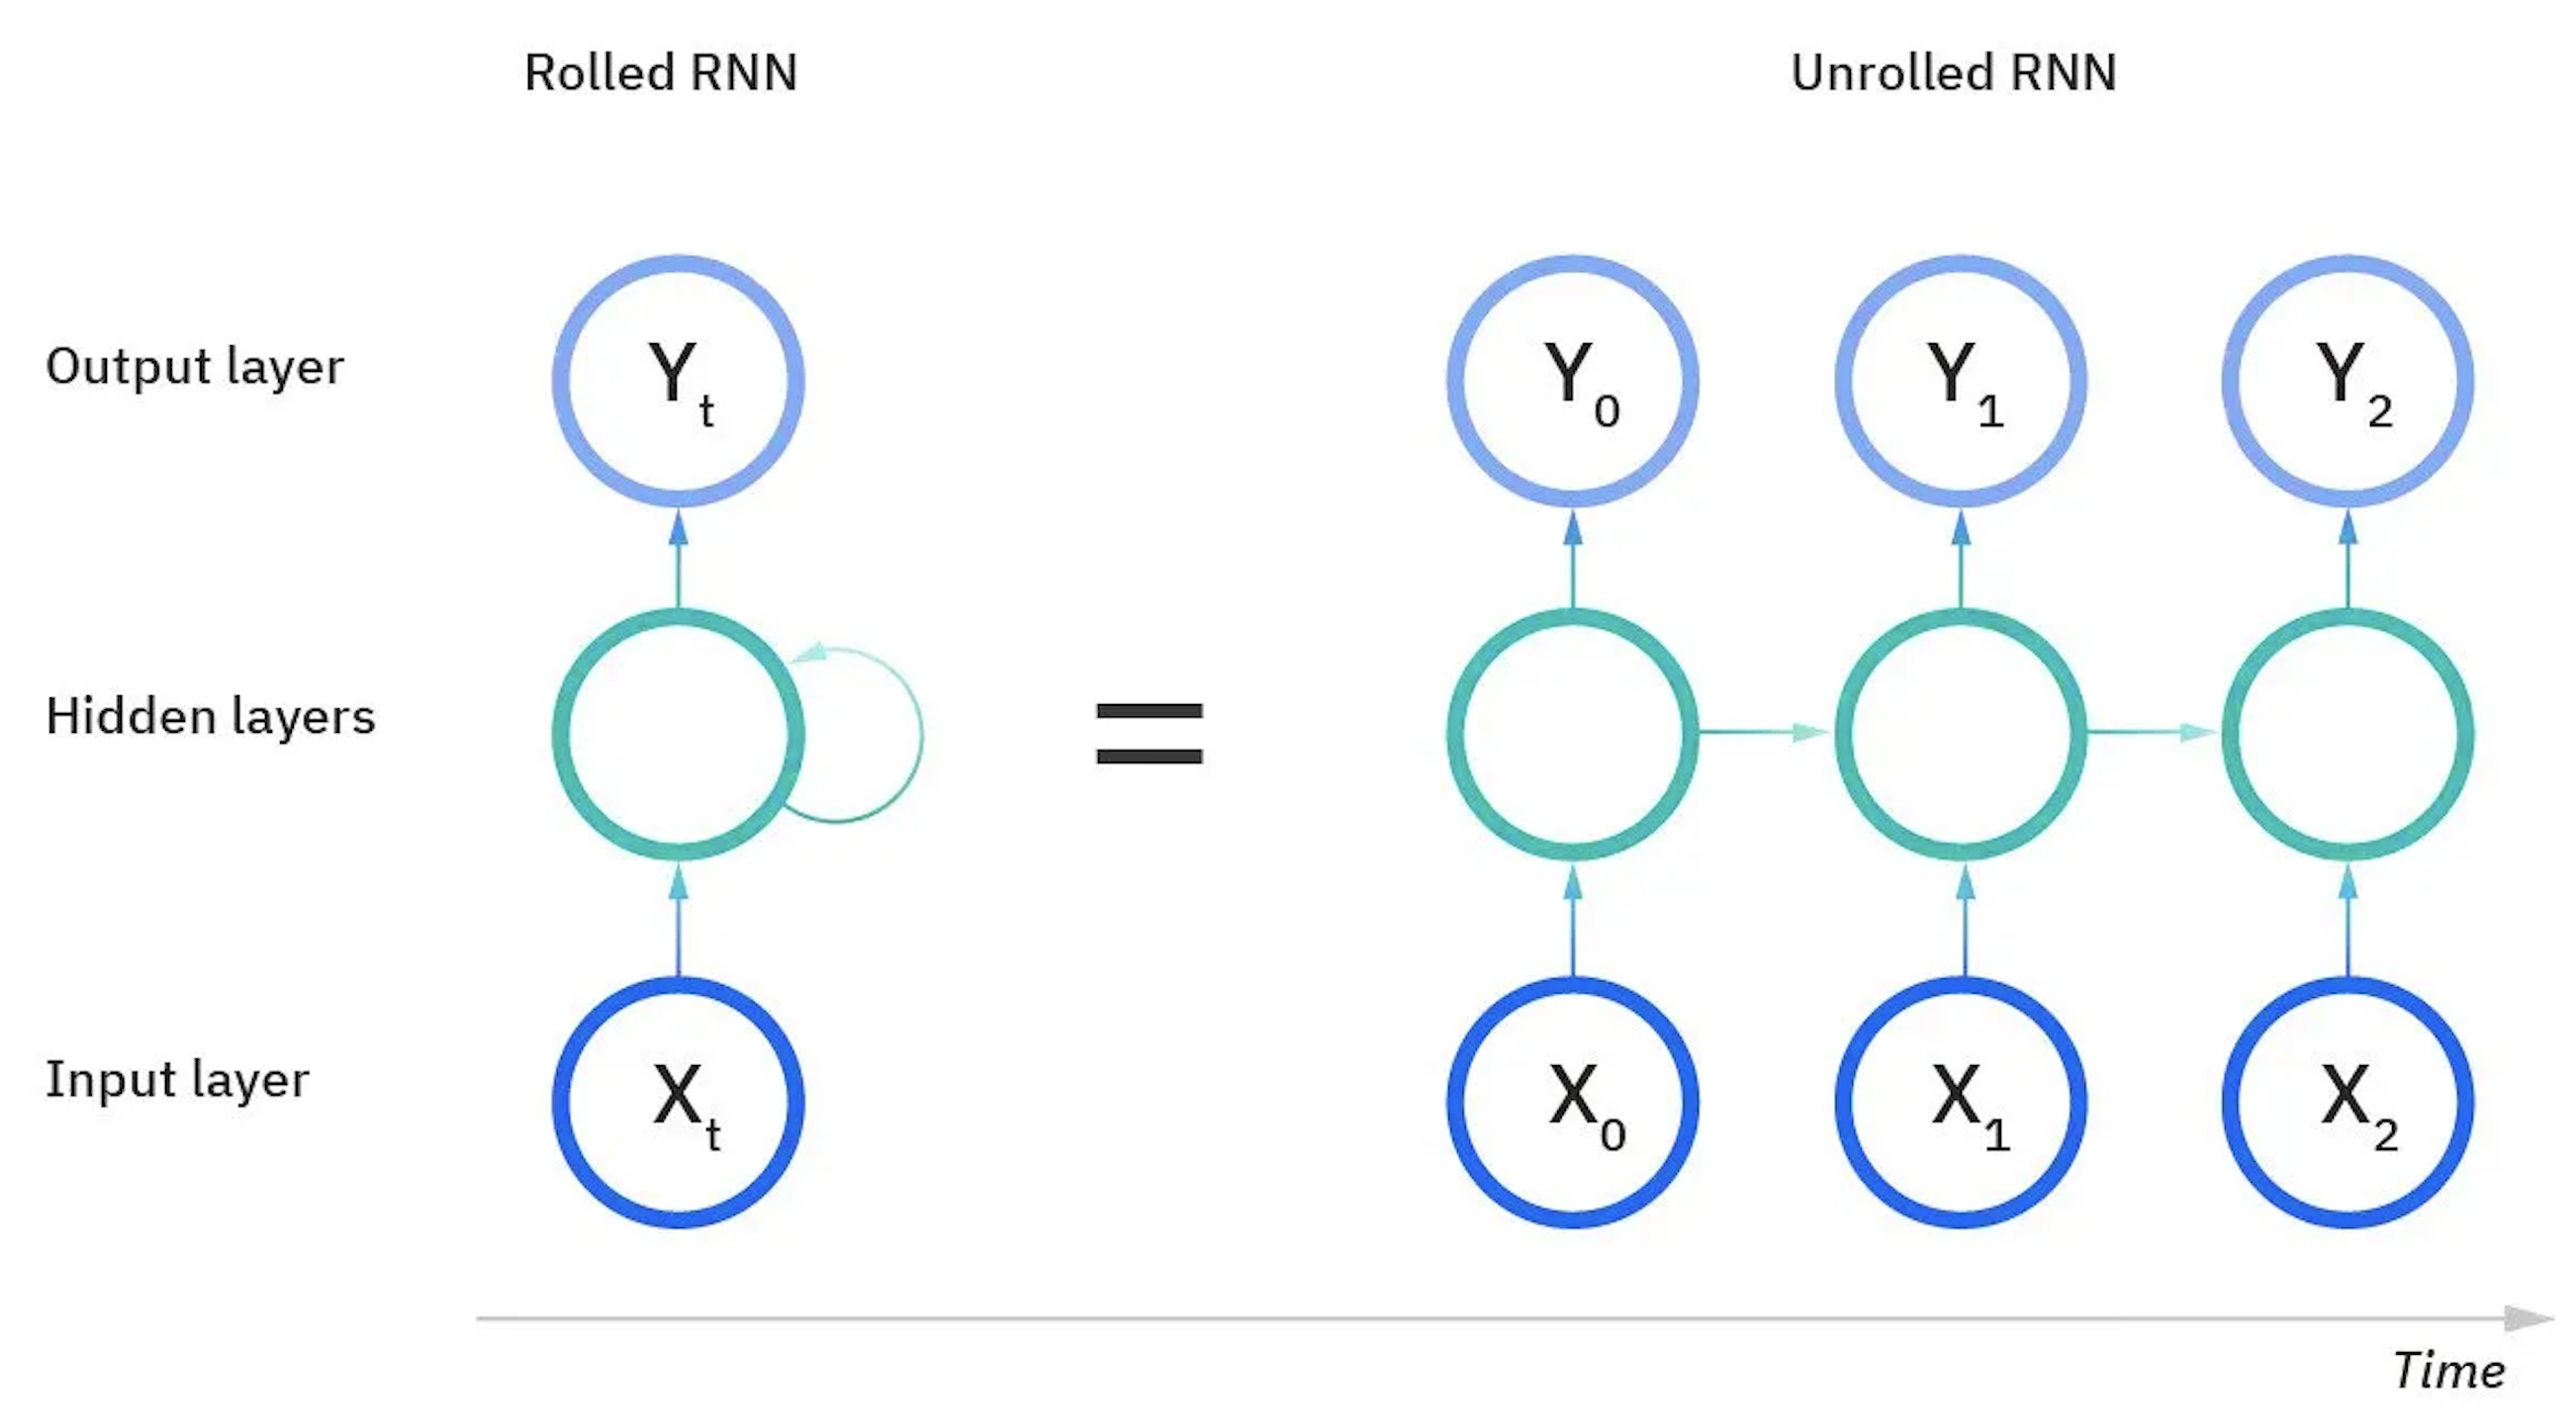
\includegraphics[width=0.70\textwidth]{figure/RNNRoll.png}
\caption{Rappresentazione schematica di una Recurrent Neural Network, nella versione "arrotolata" (a sinistra) e "srotolata" (a destra).}
\label{fig:rolledRNN}
\end{figure}
Per comprendere meglio il concetto, consideriamo l'espressione idiomatica inglese "feeling under the weather", comunemente usata per indicare che qualcuno è malato. L'espressione ha senso solo se le parole vengono pronunciate in quell'ordine specifico. Una RNN è in grado di interpretarla correttamente perché, elaborando ogni parola nel contesto delle precedenti, riesce a mantenere il significato dell'intera sequenza. La vista "arrotolata" della Figura~\ref{fig:rolledRNN} rappresenta l'intera rete come una singola entità che incorpora memoria. La vista "srotolata" invece mostra i diversi \textit{timestep}, ognuno dei quali corrisponde a un'istanza temporale della rete (ad esempio: "I", "love", "recurrent", "neural"). Ogni nodo tiene conto dello stato nascosto accumulato nel tempo per predire il token successivo, come "networks!".

\subsection{La cella di ricorrenza}

La caratteristica distintiva delle RNN è la presenza di una struttura ricorsiva che consente di mantenere uno \textit{stato nascosto} (\textit{hidden state}) lungo la sequenza (Figura~\ref{fig:recurrency_cell}). A ogni istante temporale, la rete riceve l'input corrente e lo stato nascosto precedente, aggiornando lo stato attuale tramite una funzione parametrizzata.
\begin{figure}
    \centering
    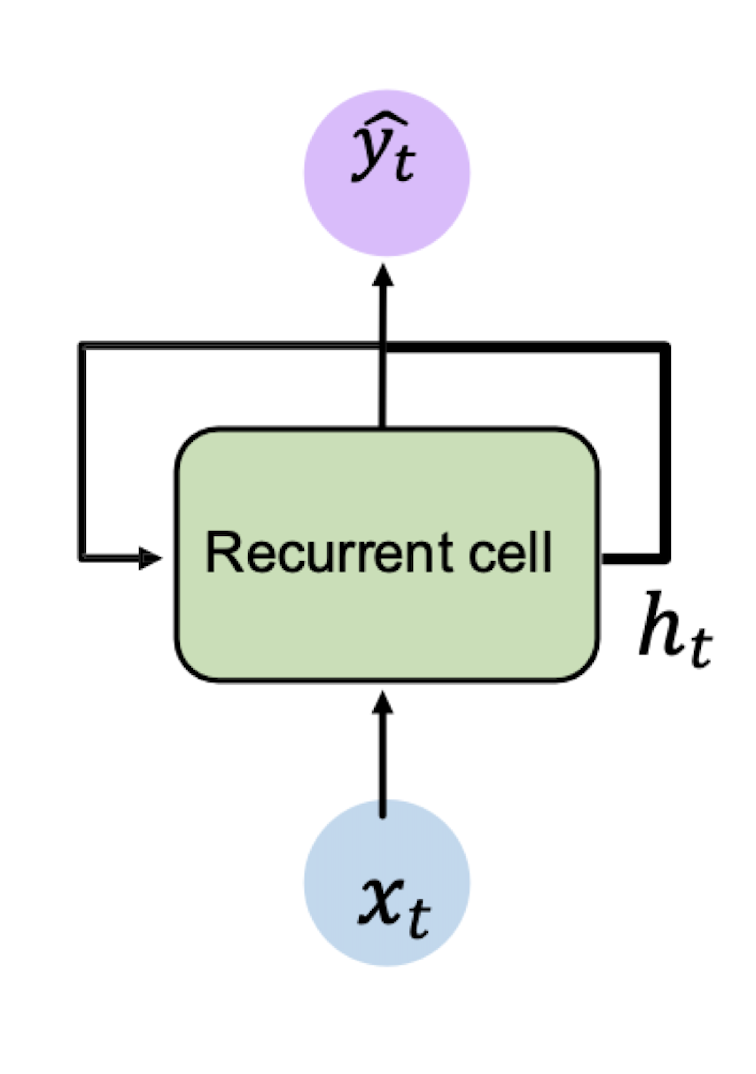
\includegraphics[width=0.32\textwidth]{figure/Recurrency_RNN.png}
    \caption{Rappresentazione della cella di ricorrenza, che integra input corrente e stato precedente attraverso la catena di retroazione.}
    \label{fig:recurrency_cell}
\end{figure}
Questo comportamento si può formalizzare tramite la seguente equazione:
\begin{equation}
    h_t = f_W(x_t, h_{t-1})
\end{equation}

Dove:
\begin{itemize}
    \item $h_t$ rappresenta lo stato nascosto corrente,
    \item $x_t$ è l'input al tempo $t$,
    \item $h_{t-1}$ è lo stato precedente,
    \item $f_W$ è una funzione non lineare parametrizzata dai pesi $W$.
\end{itemize}

Un esempio semplificato di utilizzo in pseudocodice Python è il seguente:
\vspace{0.5em}
\begin{python}
my_rnn = RNN()
hidden_state = [0, 0, 0, 0]

sentence = ["I", "love", "recurrent", "neural"]
for word in sentence:
    prediction, hidden_state = my_rnn(word, hidden_state)

nextWordPrediction = prediction
# >>> "networks!"
\end{python}
\vspace{0.5em}
Matematicamente, l'aggiornamento dello stato nascosto e il calcolo dell'output possono essere espressi così:
\begin{equation}
    h_t = \tanh(W_{hh}^T\,h_{t-1} + W_{xh}^T\,x_t) \qquad \hat{y}_t = W_{hy}^T\,h_t
\end{equation}

Come visibile nella Figura~\ref{fig:rolledRNN}, una RNN può essere vista come una rete "srotolata" nel tempo, dove ogni copia della cella condivide i medesimi parametri, ma riceve input e stato differenti. Questo riduce il carico computazionale rispetto a una rete profonda convenzionale e consente di modellare sequenze con efficienza. Inoltre, questa struttura consente di valutare la funzione di costo per ciascun intervallo temporale, rendendo esplicito come il modello gestisca la dipendenza tra istanti.

\subsection{Modellazione della sequenza}

La modellazione temporale può variare in base al tipo di task e al modo in cui si desidera produrre l'output. In Figura~\ref{fig:seqMod} sono illustrate diverse strategie:

\begin{itemize}
    \item \textbf{Many-to-One}: intera sequenza come input e un solo output finale (es. sentiment analysis);
    \item \textbf{One-to-Many}: un input iniziale e sequenza di output (es. image captioning);
    \item \textbf{Many-to-Many}: input e output sequenziali (es. machine translation).
\end{itemize}

\begin{figure}
    \centering
    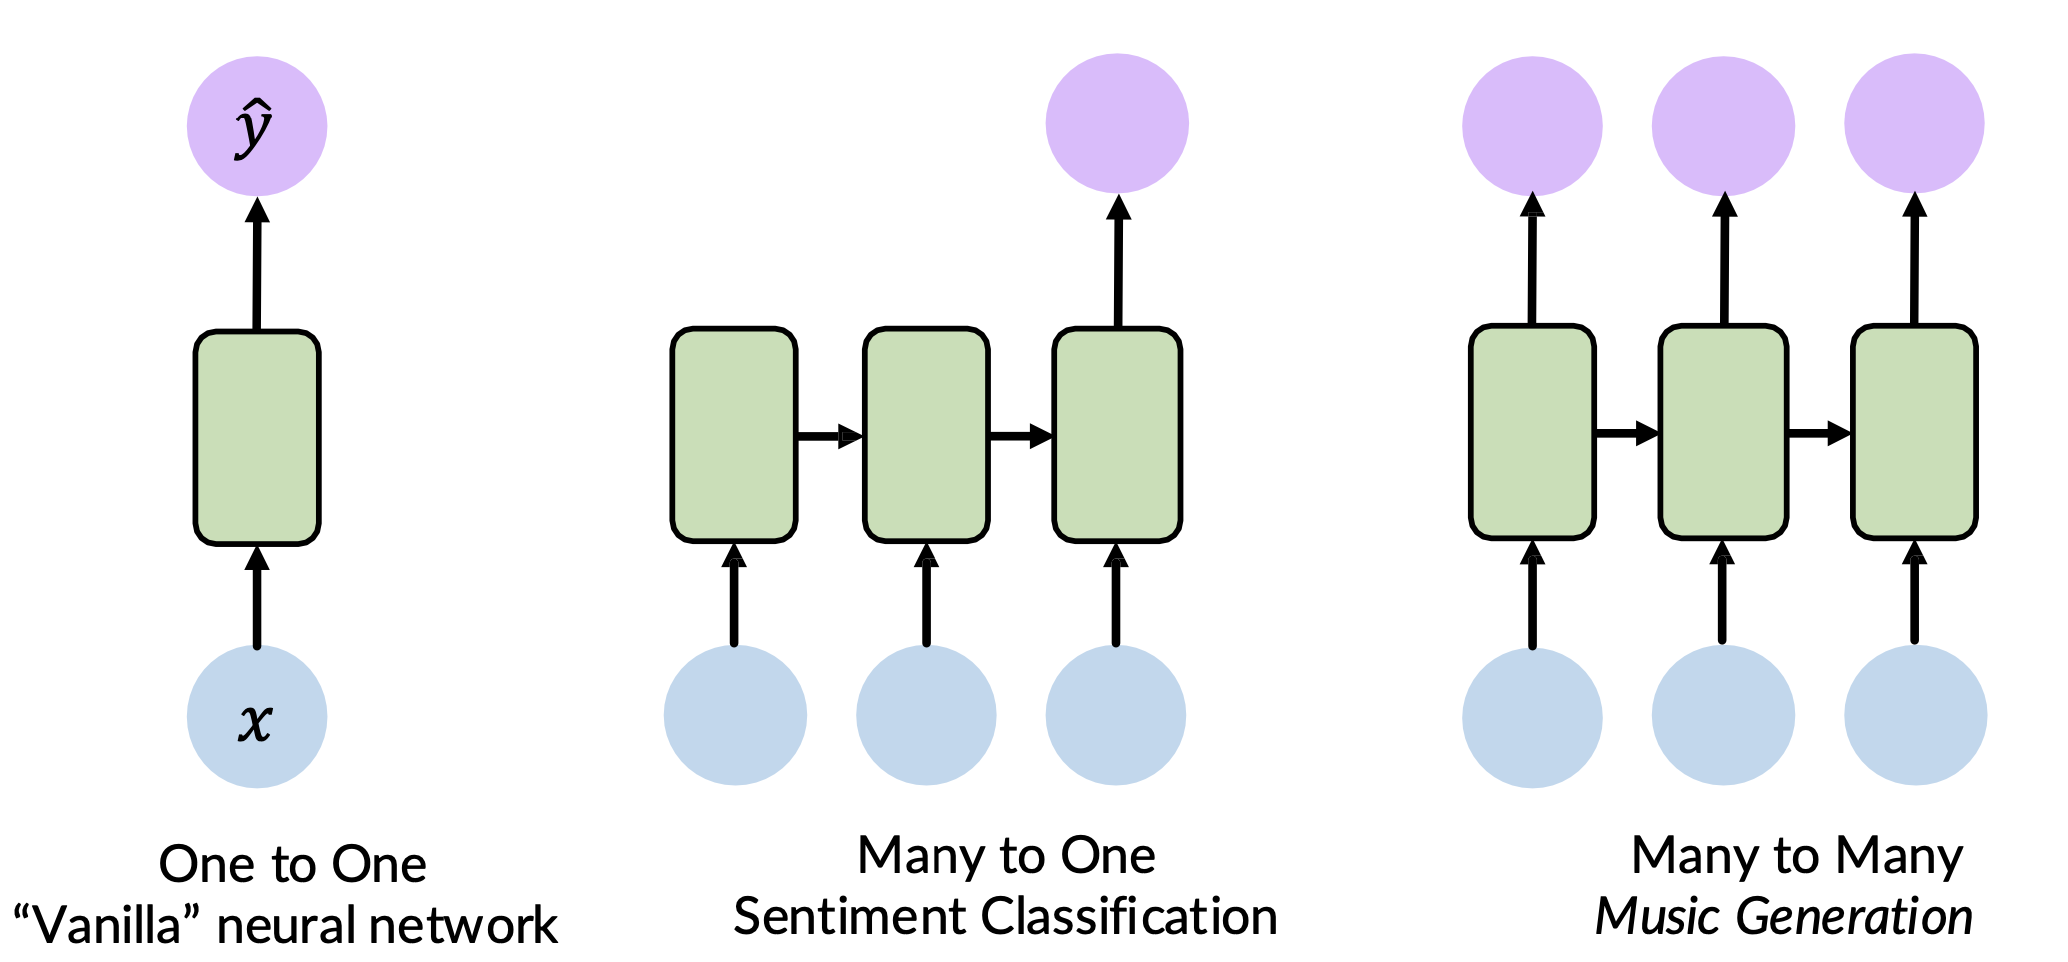
\includegraphics[width=0.85\textwidth]{figure/SequenceModeling.png}
    \caption{Esempi di modellazione della sequenza in RNN, adattabili al tipo di problema.}
    \label{fig:seqMod}
\end{figure}

\section{Backpropagation Through Time}

Quando si applica l'algoritmo di backpropagation a una RNN, lo si estende lungo la dimensione temporale: tale tecnica prende il nome di \textbf{Backpropagation Through Time} (BPTT). A ogni istante, la rete produce un output e aggiorna lo stato nascosto; durante la retropropagazione, vengono calcolati i gradienti a ritroso su tutti i \textit{timestep}, condividendo i pesi e sommando i contributi al gradiente.

\begin{equation}
    \frac{\partial L}{\partial W_{hh}} = \sum_{t = 1}^T \frac{\partial L_t}{\partial W_{hh}}
\end{equation}

Tuttavia, poiché lo stato nascosto $h_t$ dipende ricorsivamente da tutti gli stati precedenti, la derivata totale si espande in una lunga catena:
\begin{equation}
    \frac{\partial L}{\partial W} = \sum_{t=1}^T \frac{\partial L_t}{\partial h_t} \cdot \frac{\partial h_t}{\partial h_{t-1}} \cdots \frac{\partial h_1}{\partial W}
\end{equation}

\begin{figure}[!ht]
\centering
\begin{tikzpicture}[
  rnn/.style={draw, rectangle, rounded corners=5pt, minimum height=1.2cm, minimum width=1.8cm, fill=blue!10},
  arrowfwd/.style={->, thick, blue},
  arrowbwd/.style={->, thick, red, dashed},
  every node/.style={font=\small}
]

\node[rnn] (rnn0) at (0,0) {RNN$_0$};
\node[rnn, right=of rnn0] (rnn1) {RNN$_1$};
\node[rnn, right=of rnn1] (rnn2) {RNN$_2$};

\node[above=0.6cm of rnn0] (x0) {$x_0$};
\node[above=0.6cm of rnn1] (x1) {$x_1$};
\node[above=0.6cm of rnn2] (x2) {$x_2$};

\node[below=0.6cm of rnn0] (y0) {$\hat{y}_0$};
\node[below=0.6cm of rnn1] (y1) {$\hat{y}_1$};
\node[below=0.6cm of rnn2] (y2) {$\hat{y}_2$};

\draw[arrowfwd] (x0) -- (rnn0);
\draw[arrowfwd] (x1) -- (rnn1);
\draw[arrowfwd] (x2) -- (rnn2);

\draw[arrowfwd] (rnn0) -- (rnn1);
\draw[arrowfwd] (rnn1) -- (rnn2);

\draw[arrowfwd] (rnn0) -- (y0);
\draw[arrowfwd] (rnn1) -- (y1);
\draw[arrowfwd] (rnn2) -- (y2);

\draw[arrowbwd] (rnn2.south west) to[out=210,in=330] (rnn1.south east);
\draw[arrowbwd] (rnn1.south west) to[out=210,in=330] (rnn0.south east);

\end{tikzpicture}
\caption{Illustrazione della Backpropagation Through Time (BPTT), in cui gli errori si propagano all’indietro lungo la sequenza temporale.}
\end{figure}

Questa struttura porta inevitabilmente a due problemi noti:
\begin{itemize}
    \item \textbf{Vanishing Gradient:} i gradienti si riducono esponenzialmente man mano che si propaga l’errore, impedendo l’apprendimento delle dipendenze a lungo termine.
    \item \textbf{Exploding Gradient:} i gradienti crescono esponenzialmente, destabilizzando l’ottimizzazione.
\end{itemize}

In entrambi i casi, il modello fatica a gestire sequenze molto lunghe o con relazioni temporali distanti. Per risolvere queste problematiche, sono state introdotte le \textbf{Gated Cells}, che vedremo nella prossima sezione.

\section{Gated Cell}
L'idea alla base delle \textbf{Gated Cell} è quella di utilizzare unità ricorrenti più sofisticate, in grado di controllare dinamicamente quali informazioni devono essere mantenute o dimenticate lungo la sequenza temporale. Questo approccio risolve i limiti delle RNN standard nel memorizzare informazioni a lungo termine. Nel 1997, Hochreiter e Schmidhuber introdussero le \textit{Long Short Term Memory} (LSTM), che grazie a strutture semplici ma potenti — come moduli lineari e logistici con operazioni moltiplicative — riuscivano a decidere quando scrivere, leggere o conservare un'informazione in memoria, a seconda dello stato di specifici \textit{gate}. Diverse architetture implementano queste logiche con variazioni e nomi differenti. In questo capitolo ci concentreremo su due tra le più diffuse: le \textbf{Long Short Term Memory} (LSTM) e le \textbf{Gated Recurrent Unit} (GRU).

\begin{figure}[!ht]
    \centering
    \begin{tikzpicture}[scale=0.8]
    \node[draw=black, fill=darkpastelgreen!60, text=white, rounded corners=15pt, thick, minimum width=6cm, minimum height=3cm, align=center, font=\bfseries\large] 
    at (0,0) {Gated cell\\LSTM, GRU, etc...};
    \end{tikzpicture}
\end{figure}

\subsection{Long Short Term Memory Networks}
In una RNN classica, i blocchi ripetuti sono costituiti da semplici nodi computazionali. Le LSTM, invece, introducono una struttura interna più articolata (Figura~\ref{fig:LSTMSchema}), capace di gestire efficacemente il flusso informativo nel tempo. Questa architettura permette alla rete di conservare informazioni anche per sequenze molto lunghe. In \texttt{TensorFlow}, una cella LSTM può essere facilmente implementata con il comando \texttt{tf.keras.layers.LSTM(numUnits)}. Il cuore delle LSTM sono i \textit{gate}, che regolano l'informazione tramite funzioni sigmoidi e moltiplicazioni punto a punto:

\begin{figure}
    \centering
    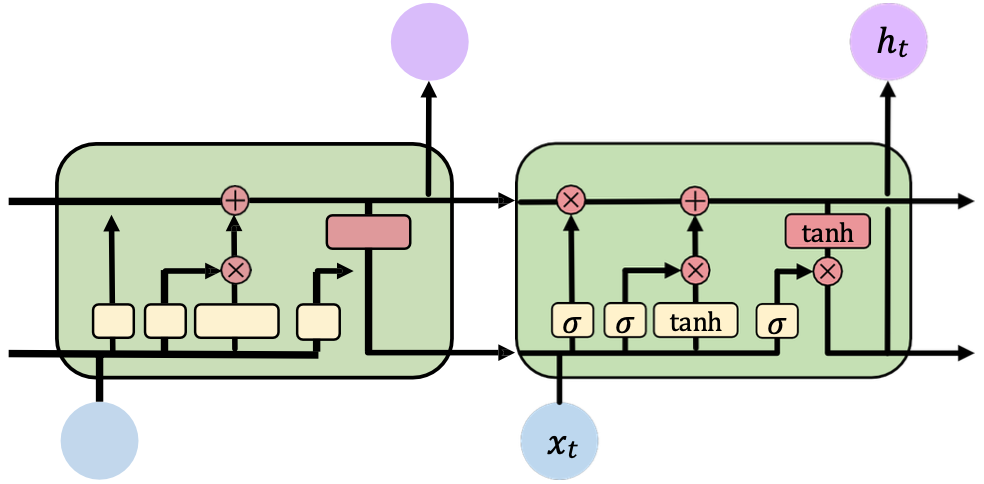
\includegraphics[width=0.85\textwidth]{figure/LSTMSchema.png}
    \caption{Rappresentazione della cella LSTM, che interagisce con un timestep precedente}
    \label{fig:LSTMSchema}
\end{figure}

\subsubsection{Forget Gate}
Il \textit{forget gate} decide quali informazioni dello stato precedente devono essere mantenute. Per farlo, combina l'input corrente con lo stato nascosto precedente, e li elabora tramite una funzione sigmoide. I valori prodotti, compresi tra 0 e 1, indicano il grado con cui ciascun elemento della memoria deve essere conservato: più vicino a 0 indica dimenticare, più vicino a 1 conservare.

\begin{figure}[!ht]
    \centering
    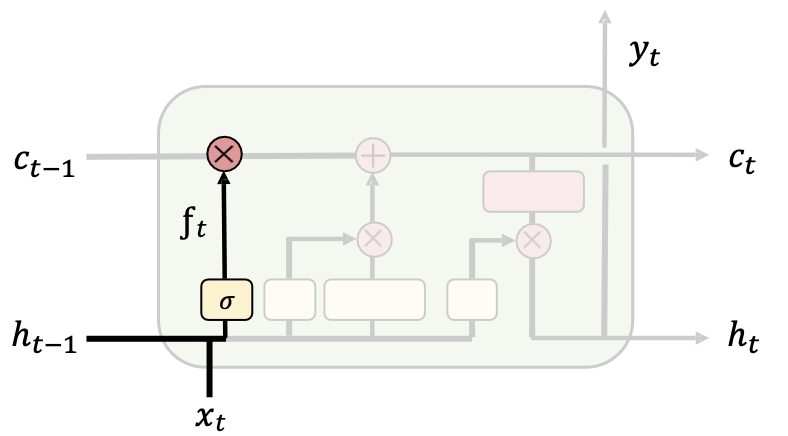
\includegraphics[width=0.55\textwidth]{figure/ForgetLSTM.png}
    \caption{Rappresentazione del gate Forget della cella LSTM}
    \label{fig:LSTMForget}
\end{figure}

\subsubsection{Store (o Input Gate)}
Lo \textit{store gate}, o \textit{input gate}, determina quali nuove informazioni devono essere aggiunte alla memoria della cella. Anche qui, input e stato nascosto precedente sono elaborati da due percorsi:
\begin{itemize}
    \item Una funzione sigmoide, che seleziona le componenti informative da aggiornare;
    \item Una funzione $\tanh$, che normalizza i nuovi valori da memorizzare in un intervallo tra -1 e 1.
\end{itemize}
Il prodotto tra questi due risultati indica quali parti della nuova informazione saranno effettivamente aggiunte allo stato interno.

\begin{figure}[!ht]
    \centering
    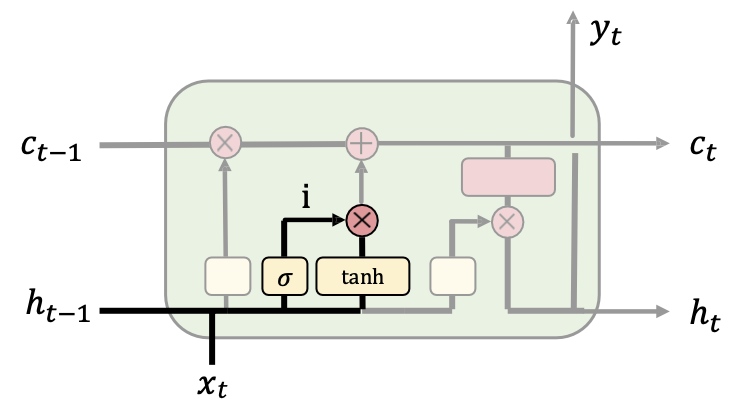
\includegraphics[width=0.55\textwidth]{figure/StoreLSTM.png}
    \caption{Rappresentazione del gate Store della cella LSTM}
    \label{fig:LSTMStore}
\end{figure}

\subsubsection{Update Gate}
L’\textit{update} rappresenta il cuore del funzionamento della LSTM. Qui lo stato della cella viene aggiornato combinando:
\begin{itemize}
    \item Lo stato precedente, pesato dal forget gate;
    \item Le nuove informazioni, selezionate dallo store gate.
\end{itemize}
La somma dei due produce il nuovo stato della cella, considerando tutti i valori che adesso la rete neurale ritiene rilevanti.

\begin{figure}[!ht]
    \centering
    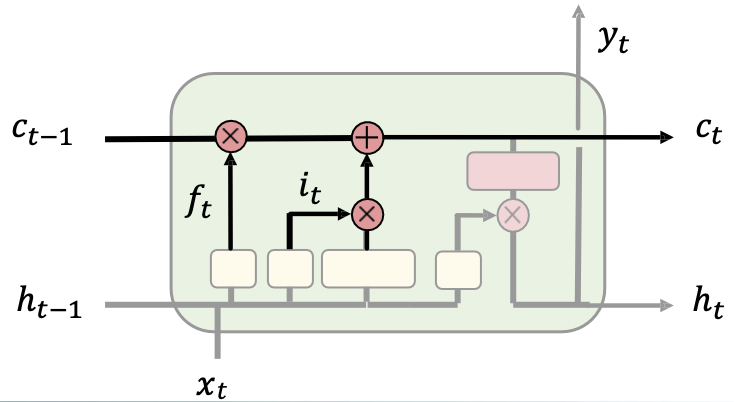
\includegraphics[width=0.55\textwidth]{figure/UpdateLSTM.png}
    \caption{Rappresentazione del gate Update della cella LSTM}
    \label{fig:LSTMUpdate}
\end{figure}

\subsubsection{Output Gate}
Infine, l’\textit{output gate} decide quale informazione deve essere trasmessa al prossimo timestep, ovvero il nuovo stato nascosto. L'input e lo stato nascosto precedente vengono processati da una funzione sigmoide, mentre lo stato interno aggiornato attraversa una funzione $\tanh$. Il prodotto punto a punto di questi due risultati rappresenta l'output finale della cella.

\begin{figure}[!ht]
    \centering
    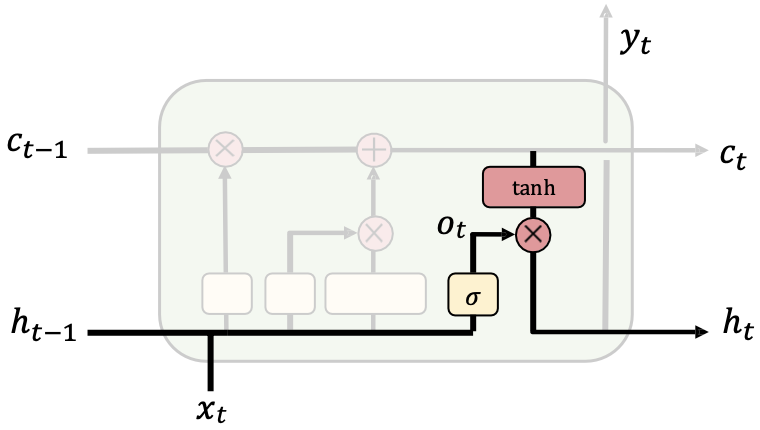
\includegraphics[width=0.55\textwidth]{figure/OutputLSTM.png}
    \caption{Rappresentazione del gate Output della cella LSTM}
    \label{fig:LSTMOutput}
\end{figure}

\subsubsection{Backpropagation solved}
Grazie alla struttura interna della cella, le LSTM mitigano i problemi del gradiente che scompare o esplode: le informazioni vengono propagate tramite somme e moltiplicazioni punto a punto, evitando lunghe catene di moltiplicazioni tra matrici che potrebbero alterare drasticamente i gradienti.

\subsection{Gated Recurrent Unit}
Le \textbf{Gated Recurrent Unit} (GRU) sono una versione semplificata delle LSTM, ma mantengono ottime capacità di apprendimento del contesto. Le GRU impiegano due gate:
\begin{itemize}
    \item Il \textbf{reset gate}, che decide quanto dello stato precedente deve essere dimenticato;
    \item L’\textbf{update gate}, che controlla quanto del nuovo contenuto deve essere incorporato nel nuovo stato nascosto.
\end{itemize}

\begin{figure}[hbtp]
    \centering
    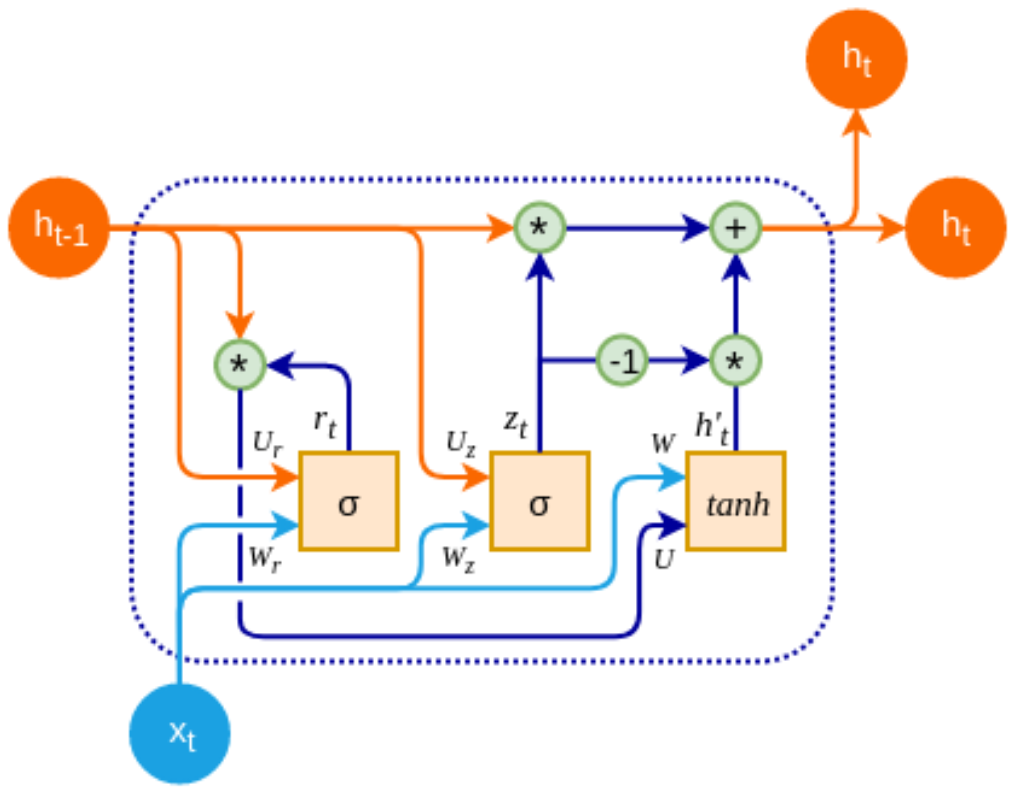
\includegraphics[width=0.70\textwidth]{figure/GNU.png}
    \caption{Rappresentazione della cella GNU, con tutti i suoi gate}
    \label{fig:GNU}
\end{figure}

\subsection{Applicazioni}
Le RNN — e in particolare le loro varianti LSTM e GRU — trovano impiego in moltissimi ambiti: generazione musicale, analisi del sentimento, traduzione automatica, e altro ancora. Queste applicazioni si basano spesso sul \textbf{meccanismo dell'attenzione}. Il \textit{meccanismo dell’attenzione} consente alla rete di concentrarsi sulle parti più rilevanti della sequenza, simulando l'apprendimento umano del linguaggio. Proprio come un bambino associa significati alle parole tramite contesto e ripetizione, l’attenzione permette alla rete di catturare relazioni semantiche tra parole, senza alcuna codifica esplicita delle regole grammaticali.\marginpar{\href{https://arxiv.org/pdf/1706.03762}{"Attention Is All You Need", by Ashish Vaswani et al. (2017)~\cite{vaswani2017attention}}}A ogni parola è associato un vettore numerico molto lungo. Questi vettori possono essere visualizzati come punti in uno spazio semantico, la cosa straordinaria è che la vicinanza tra punti, riflette affinità semantiche tra parole.
\begin{figure}
    \centering
    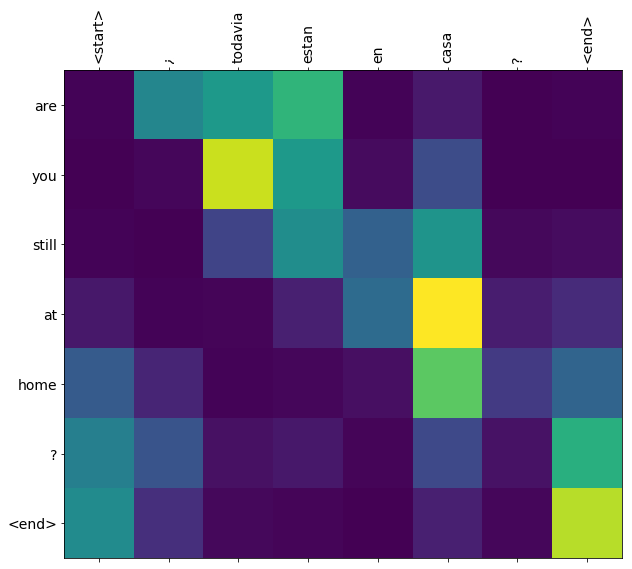
\includegraphics[width=0.50\textwidth]{figure/AttentionEx.png}
    \caption{Rappresentazione del meccanismo dell'attenzione in un compito di traduzione: le zone più gialle indicano alta probabilità di corrispondenza tra parole.}
    \label{fig:AttEx}
\end{figure}
L'algoritmo dell'attenzione calcola il prodotto scalare tra ogni parola e tutte le altre, identificando le relazioni più rilevanti. Questo approccio non è limitato al linguaggio: può essere applicato anche a note musicali, pixel o altri dati sequenziali.

\subsection{Bi-LSTM}
Le \textbf{Bi-LSTM} (Bidirectional LSTM) estendono le LSTM standard eseguendo due elaborazioni:
\begin{enumerate}
    \item Una in avanti, dalla prima all'ultima parola;
    \item Una all’indietro, dall’ultima alla prima parola.
\end{enumerate}
I risultati vengono poi combinati (di solito tramite concatenazione o somma), fornendo un contesto bidirezionale. Questo è particolarmente utile, ad esempio, per prevedere una parola mancante in una frase: serve sia il contesto passato che futuro.
\begin{figure}
    \centering
    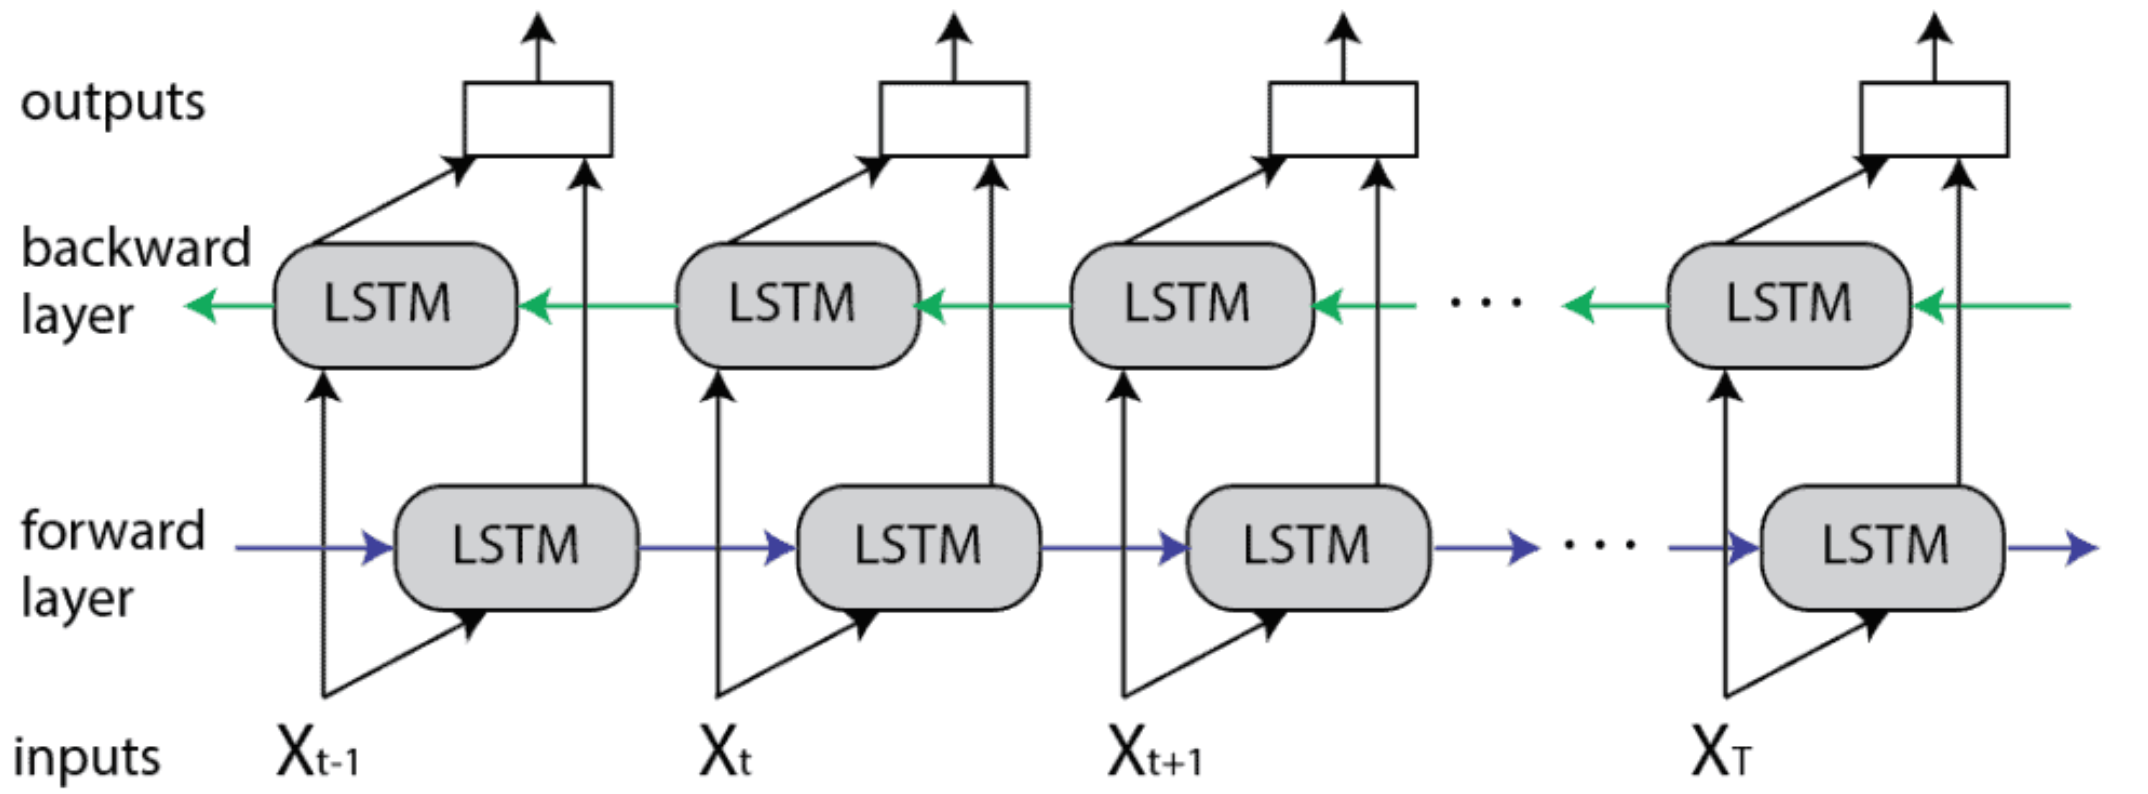
\includegraphics[width=0.8\textwidth]{figure/Bi-LSTM.png}
    \caption{Architettura di una Bi-LSTM}
    \label{fig:bilstm}
\end{figure}
Questa potenza ha un costo: due reti LSTM devono essere addestrate simultaneamente, il che comporta un maggiore uso di memoria e tempi di addestramento più lunghi.

\subsection{Bi-LSTM con Attenzione}
Un limite delle Bi-LSTM è che, nonostante processino la sequenza in entrambe le direzioni, alla fine restituiscono un singolo vettore che riassume l'intera sequenza. Questo può essere problematico se la sequenza è molto lunga o se alcune parti sono più rilevanti di altre. Il \textbf{meccanismo dell'attenzione} risolve questo problema: assegna un peso $\alpha_t$ a ciascun passo temporale, indicando quanto ogni stato nascosto deve contribuire all'output finale.

\begin{figure}[hbtp]
    \centering
    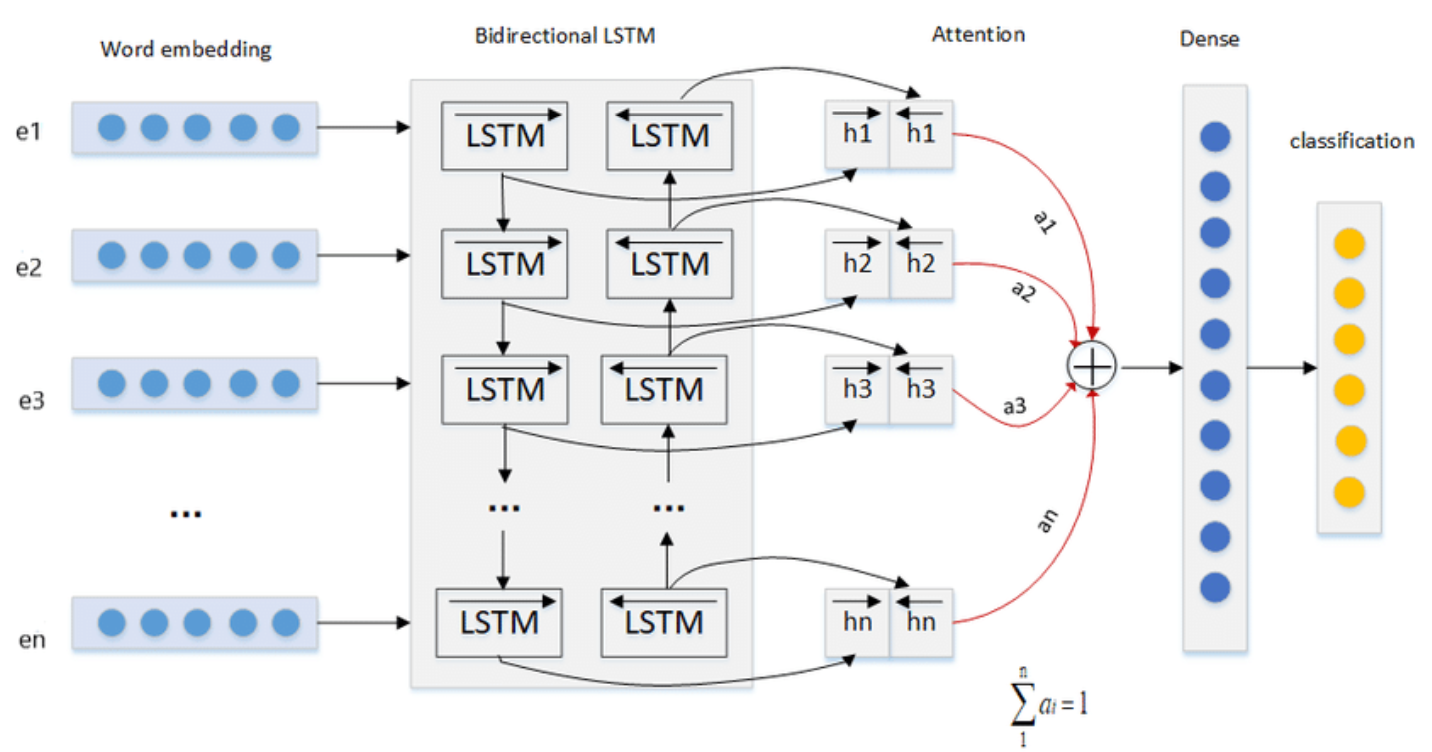
\includegraphics[width=0.8\textwidth]{figure/Bi-LSTMAtt.png}
    \caption{Architettura di una Bi-LSTM con meccanismo di attenzione}
    \label{fig:bilstmatt}
\end{figure}
\chapter{Migliorare la Generalizzazione}

La \textbf{Generalizzazione} rappresenta il cuore del Machine Learning: un modello non deve semplicemente memorizzare i dati del training set, ma dev’essere in grado di effettuare previsioni accurate anche su esempi mai visti prima. Per questo motivo, i dataset sono solitamente suddivisi in training set e test set: quest’ultimo non viene mostrato al modello durante l’addestramento, ma serve a valutare la capacità di generalizzazione. Nel Deep Learning, la questione diventa ancora più delicata: i modelli hanno un’elevata capacità espressiva e possono facilmente adattarsi in modo eccessivo ai dati di addestramento, fenomeno noto come \textbf{Overfitting}.

\section{Overfitting}

L’\textbf{Overfitting} si verifica quando un modello si adatta troppo ai dati di training, arrivando a modellare anche rumore e irregolarità accidentali, spesso dovute a errori di campionamento. In questi casi, il modello perde la capacità di distinguere tra regolarità significative e dettagli irrilevanti. Questo accade in particolare con modelli molto flessibili, che hanno una capacità sufficiente per apprendere qualsiasi cosa, incluse le fluttuazioni casuali dei dati.

\begin{quote}
\emph{"Se un modello è abbastanza potente da spiegare tutto, finirà per spiegare anche ciò che non è rilevante."}
\end{quote}

\begin{Osservazione}
    Visualizzare il fenomeno dell'overfitting, basta immaginare una persona che si veste con delle taglie di vestiti diverse, se un vestito risulta essere troppo aderente parleremo di overfitting, quando un vestito è troppo largo parleremo di underfitting.
\end{Osservazione}

\subsection{Prevenire l’Overfitting}

Per prevenire l’Overfitting, si possono adottare tre strategie principali, oltre a quelle già viste nel corso base di Machine Learning:

\begin{itemize}
    \item \textbf{Espandere il dataset}, ovvero ottenere più dati. È la soluzione più efficace, ma spesso difficile da realizzare nella pratica;
    \item \textbf{Utilizzare modelli con capacità adeguata}, evitando reti troppo semplici (Underfitting) o troppo complesse (Overfitting);
    \item \textbf{Combinare più modelli} (ensemble), utilizzando architetture diverse o addestramenti su sottoinsiemi dei dati.
\end{itemize}

L’espansione del dataset aiuta a ridurre il rumore e aumenta la significatività statistica. I modelli troppo complessi rischiano l’Overfitting, mentre quelli troppo semplici non riescono a catturare la struttura dei dati (Underfitting). Infine, l’ensembling permette di mediare tra i diversi comportamenti, bilanciando bias e varianza, questa possibilità viene effettuato utilizzando tecniche di \textit{Bagging} e di \textit{Boosting}, su cui ci soffermeremo più avanti.

\section{Limitare la capacità di un modello}

La capacità di un modello può essere controllata in diversi modi:

\begin{itemize}
    \item \textbf{Architettura:} definizione del numero di layer e neuroni;
    \item \textbf{Early Stopping:} interrompere l’addestramento prima che inizi l’Overfitting;
    \item \textbf{Weight Decay:} aggiungere una penalizzazione ai pesi grandi tramite regolarizzazione L1 o L2;
    \item \textbf{Noise Injection:} aggiungere rumore agli input o alle attivazioni per migliorare la robustezza;
    \item \textbf{Dropout:} È una delle forme di regolarizzazione più potenti e specifiche per il Deep Learning. Durante ogni passo dell'addestramento, una frazione casuale di neuroni viene temporaneamente "spenta" (le loro uscite vengono impostate a zero).
\end{itemize}

Tutte queste tecniche mirano a ridurre la complessità effettiva del modello, favorendo una maggiore capacità di generalizzazione,vediamole ora meglio.

\subsection{Early Stopping}

L’\textbf{Early Stopping} è una tecnica che interrompe l’addestramento nel momento in cui il modello inizia a sovra-adattarsi ai dati. Nelle prime fasi, i pesi sono piccoli e i neuroni operano nella regione lineare; col progredire dell’allenamento, i pesi aumentano, i neuroni entrano nella regione non lineare e il modello diventa più potente, rischiando però l’Overfitting. Fermare l’allenamento nel momento opportuno consente di mantenere una buona capacità predittiva. È pratica comune utilizzare un \textbf{Validation Set} per monitorare l’andamento dell’errore e decidere quando arrestare l’addestramento.

\subsection{Weight Decay}

La regolarizzazione L2 introduce un termine additivo nella funzione di costo per penalizzare i pesi grandi:

\begin{equation}
J(\theta) = \mathcal{L}(\theta) + \lambda \sum_i \theta_i^2
\end{equation}

Questo termine forza i pesi a rimanere piccoli, evitando soluzioni troppo complesse. Il parametro $\lambda$ controlla l’intensità della penalizzazione:

\begin{itemize}
\item $\lambda$ troppo grande $\Rightarrow$ Underfitting;
\item $\lambda$ troppo piccolo $\Rightarrow$ rischio di Overfitting.
\end{itemize}

La regolarizzazione L1 $ (\sum_i |\theta_i|)$ è un’alternativa che induce \textbf{sparsità}, cioè tende a portare molti pesi a zero, dunque adoperando una sorta di selezione delle features.

\subsection{Noise Injection}

Aggiungere rumore ai dati d’ingresso o ai pesi agisce come regolarizzatore. Ad esempio aggiungendo un \textbf{rumore Gaussiano}:
\[
x_t^{(noisy)} = x_t + \mathcal{N}(0, \sigma^2)
\]
Il rumore, amplificato dai pesi, penalizza indirettamente pesi grandi. L’effetto è simile al weight decay: il modello diventa più robusto e meno dipendente da feature specifiche.

\subsection{Dropout}

Il \textbf{Dropout} è una tecnica di regolarizzazione che disattiva casualmente neuroni durante l’addestramento. Ogni forward pass attiva una sottorete diversa, riducendo la dipendenza da co-attivazioni specifiche. Con \( H \) neuroni, si campionano \( 2^H \) reti. I pesi sono condivisi, quindi ogni sottorete è fortemente regolarizzata, il dropout permette di ridurre gli adattamenti complessi tra neuroni e rafforza la robustezza della rete.
\begin{figure}
    \centering
    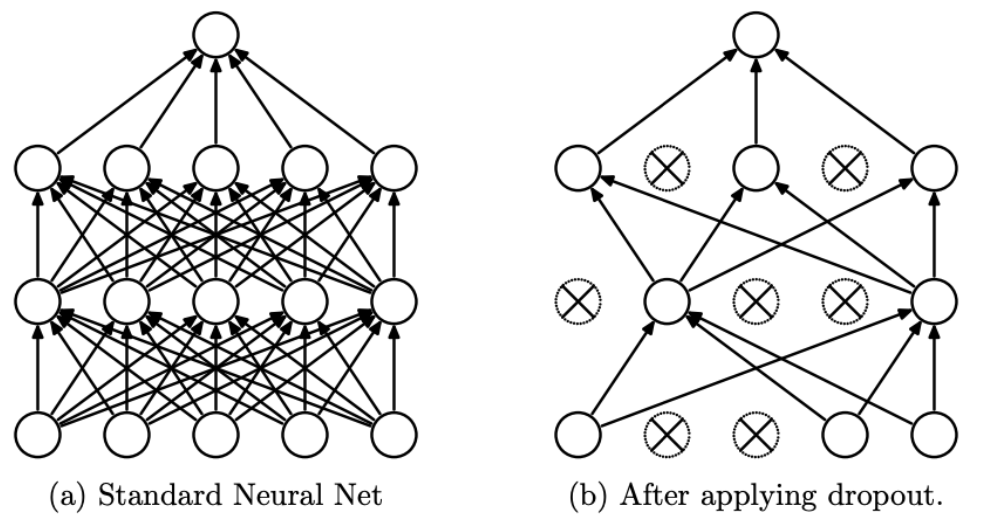
\includegraphics[width=0.85\textwidth]{figure/Dropout.png}
    \caption{Una Rete Neurale completamente connessa (a sinistra). La stessa Rete Neurale dopo che è stato applicato il Dropout (a destra).}
    \label{fig:dropout}
\end{figure}
Di conseguenza questa tecnica permette di avere due effetti principali:
\begin{enumerate}
    \item \textbf{Forza la robustezza:} I neuroni non possono fare affidamento sulla presenza di altri neuroni specifici e sono costretti a imparare feature utili e robuste in modo indipendente
    \item \textbf{Simula un ensemble:} Ad ogni iterazione, si addestra una "sottorete" diversa. Il risultato finale è un'approssimazione efficiente dell'addestramento e della media di un numero esponenziale di reti diverse che condividono i pesi.
\end{enumerate}

Pertanto il Dropout non è solo una forma di regolarizzazione numerica, ma impone una \textit{robustezza strutturale}, in cui ogni neurone dev’essere \textbf{indipendentemente utile}. Questo argomento può essere approfondito in Srivastava et al. 2014~\cite{srivastava2014dropout}.

\section{Ensembling}
Invece di cercare un singolo modello perfetto, le tecniche di ensemble combinano le previsioni di più modelli per ottenere un risultato più robusto e accurato. L'errore di un modello può essere scomposto in Bias (quanto le previsioni sono sistematicamente sbagliate) e Varianza (quanto le previsioni cambiano al variare del training set). L'ensemble è un modo potente per ridurre la varianza.

\[
\text{Errore totale} = \text{Bias}^2 + \text{Varianza} + \text{Rumore}
\]

Affinché un ensemble funzioni, i modelli che lo compongono devono essere diversi tra loro. La diversità può essere ottenuta addestrando modelli con architetture diverse, iperparametri diversi o su sottoinsiemi diversi dei dati. Le due strategie principali per creare ensemble sono:

\begin{itemize}
  \item \textbf{Bagging:} Si addestrano più modelli indipendentemente su diversi sottoinsiemi del training set, creati tramite campionamento con rimpiazzo. Le previsioni vengono poi aggregate (e.g media o voto di maggioranza). Il Bagging è particolarmente efficace nel ridurre la varianza di modelli complessi (basso bias, alta varianza);
  \item \textbf{Boosting:} Si addestrano modelli in sequenza. Ogni nuovo modello si concentra sugli errori commessi dai modelli precedenti, dando più peso agli esempi classificati erroneamente. Il Boosting è ottimo per ridurre il bias di modelli semplici (alto bias, bassa varianza).
\end{itemize}

\begin{figure}
    \centering
    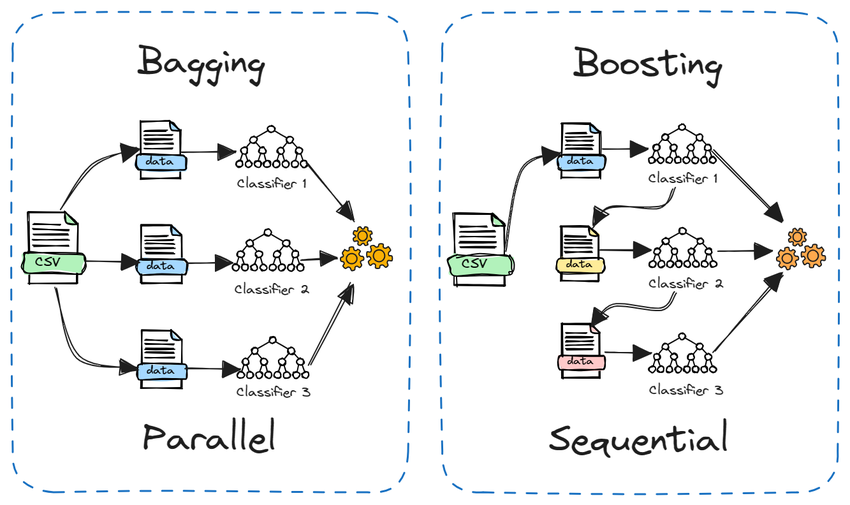
\includegraphics[width=0.6\textwidth]{figure/BagBoost.png}
    \caption{Rappresentazione dell’Ensemble tramite Bagging (modelli in parallelo) e Boosting (modelli in sequenza).}
    \label{fig:bagBoost}
\end{figure}

\section{Riepilogo delle Tecniche}
Non esiste una singola tecnica valida per ogni problema. Nella pratica, le strategie per migliorare la generalizzazione vengono spesso combinate. Ad esempio, è comune usare Data Augmentation, Weight Decay e Dropout contemporaneamente all'interno di una rete neurale. La scelta e la calibrazione di queste tecniche sono una parte fondamentale del processo di sviluppo di un modello di successo.

\begin{table}[h]
    \centering
    \caption{Strategie per migliorare la generalizzazione nei modelli di Deep Learning}
    \begin{adjustbox}{width=\textwidth}
    \begin{tabular}{@{}l|l@{}}
    \toprule
    \textbf{Tecnica} & \textbf{Descrizione} \\
    \midrule
    \textbf{Aumento dei dati} & Espandere il dataset con esempi reali o sintetici \\
    \textbf{Architettura adeguata} & Scegliere la capacità del modello con attenzione \\
    \textbf{Early Stopping} & Interrompere l’addestramento in tempo utile \\
    \textbf{Weight Decay} & Penalizzare pesi grandi nella funzione di loss \\
    \textbf{Noise Injection} & Aggiungere rumore a input o attivazioni \\
    \textbf{Ensemble} & Media di modelli diversi per ridurre la varianza \\
    \textbf{Bagging} & Campionamento con rimpiazzo per ensemble \\
    \textbf{Boosting} & Addestramento sequenziale di modelli deboli \\
    \textbf{Dropout} & Spegnere neuroni casualmente evitando adattamenti \\
    \bottomrule
    \end{tabular}
    \end{adjustbox}
\end{table}

\chapter{Autoencoder}

Un \textbf{Autoencoder} è una rete neurale progettata per apprendere una rappresentazione compressa dell’input attraverso un processo di codifica e successiva decodifica, con l’obiettivo di ricostruire fedelmente l’input stesso in output: $h_\theta (x) \approx x$. Sebbene questa formulazione possa apparire banale, il valore dell'autoencoder risiede nella sua capacità di apprendere rappresentazioni utili dei dati grazie a specifici vincoli architetturali. In particolare, l’apprendimento di una funzione identità approssimata diventa un compito non banale se si impongono vincoli strutturali quali:

\begin{enumerate}
\item \textbf{Compressione del livello nascosto}: La dimensionalità dello strato nascosto è inferiore rispetto a quella dell’input, costringendo la rete a catturare le caratteristiche più rilevanti dell’informazione.
\item \textbf{Sparsità}: Si introduce un vincolo per cui, durante la fase di training, solo un numero limitato di neuroni dello strato nascosto risulta attivo per ogni input. Ciò viene realizzato aggiungendo un termine di penalizzazione alla funzione di costo.
\end{enumerate}

\begin{figure}[h!]
\centering
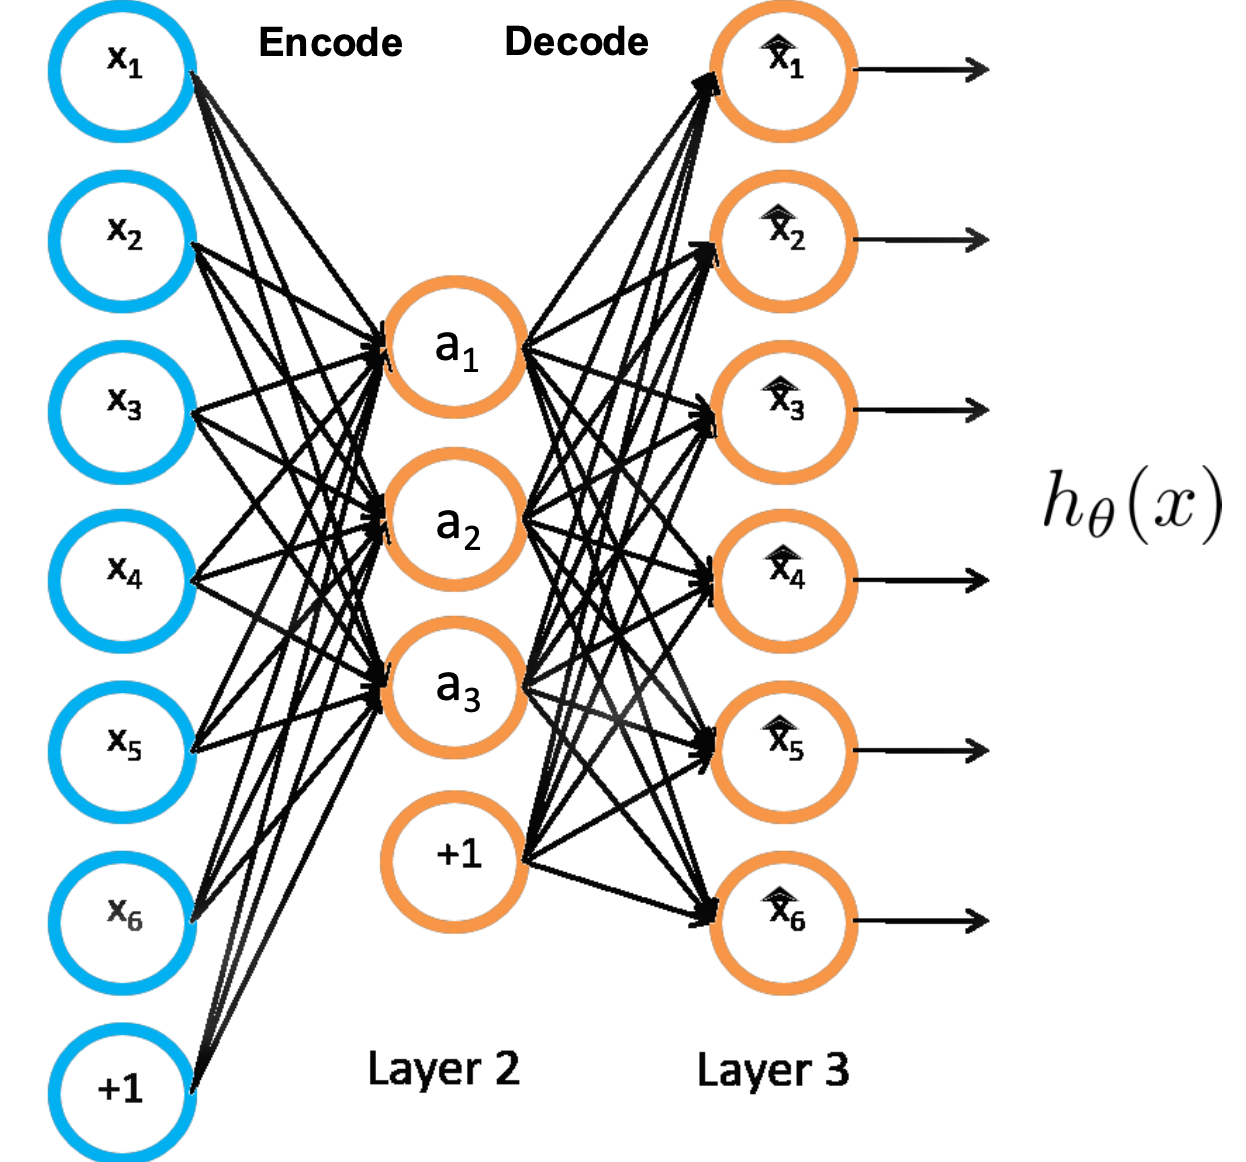
\includegraphics[width=0.5\textwidth]{figure/AAutoencoder.png}
\caption{Struttura tipica di un Autoencoder}
\label{fig:AutoEnc}
\end{figure}

\section{U-Net}

La \textbf{U-Net} è un’architettura di deep learning sviluppata specificamente per compiti di segmentazione semantica di immagini, con applicazioni rilevanti in ambito medico, come l’identificazione di lesioni o tumori. L’obiettivo è classificare ogni singolo pixel dell’immagine in una determinata categoria, restituendo una mappa binaria o multiclasse. Un esempio è illustrato in Figura~\ref{fig:cell}.

\begin{figure}[!ht]
\centering
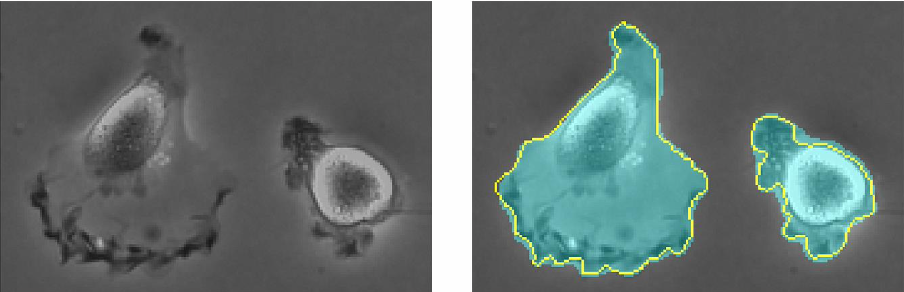
\includegraphics[width=0.75\textwidth]{figure/Cells.png}
\caption{Esempio di segmentazione semantica: a sinistra l'immagine originale, a destra la mappa segmentata. I pixel evidenziati rappresentano la classe target.}
\label{fig:cell}
\end{figure}

L’architettura della U-Net è suddivisa in tre componenti principali: \emph{Encoder}, \emph{Decoder} e \emph{Skip Connections}.

\begin{itemize}
\item \textbf{Encoder}: Composto da blocchi convoluzionali e operazioni di downsampling (es. max pooling), estrae progressivamente feature sempre più astratte.
\item \textbf{Decoder}: Costituito da operazioni di upsampling (es. up-convolutions) e convoluzioni, ricostruisce l’immagine nella sua risoluzione originale.
\item \textbf{Skip Connections}: Collegano simmetricamente gli strati dell’encoder con quelli del decoder, trasmettendo direttamente informazioni spaziali dettagliate, utili alla ricostruzione dell’output.
\end{itemize}

\begin{figure}[!ht]
\centering
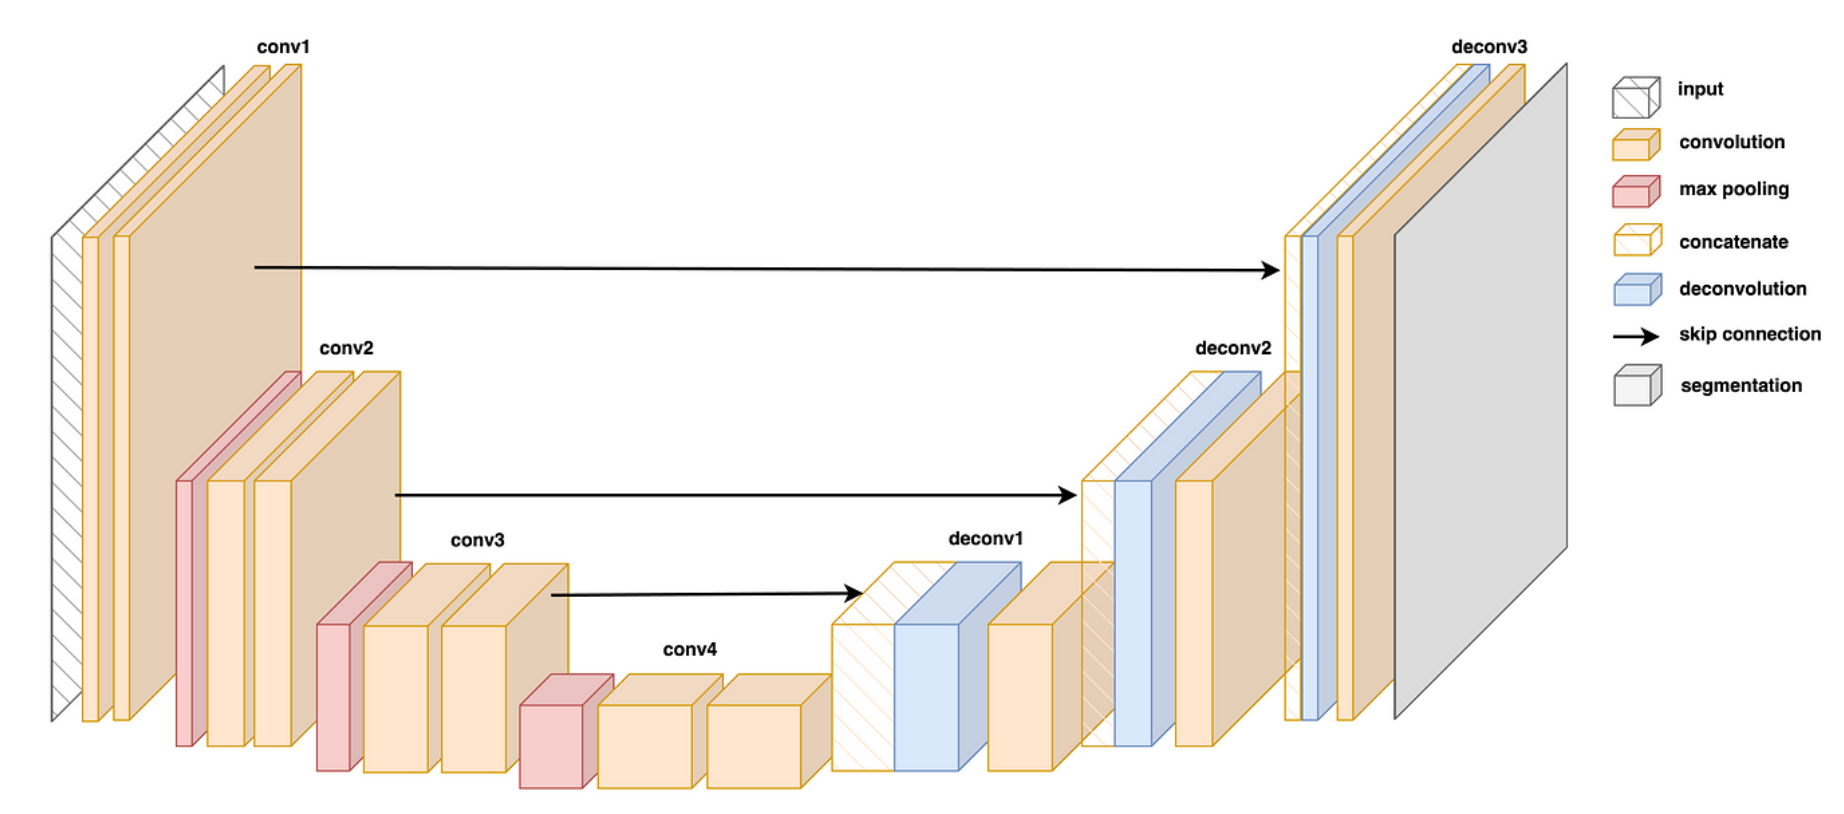
\includegraphics[width=0.85\textwidth]{figure/UNet.png}
\caption{Architettura di una U-Net}
\label{fig:unet}
\end{figure}

Durante la fase di downsampling, le informazioni spaziali precise tendono a degradarsi. Tuttavia, grazie alle skip connections, le caratteristiche di basso livello, conservate nei primi layer convoluzionali, vengono riutilizzate nel decoder per preservare la localizzazione spaziale dei dettagli. Questo migliora sensibilmente la qualità dell'output segmentato.

\section{Limitazioni degli Autoencoder}

Gli autoencoder sono efficaci per compiti di compressione, riduzione del rumore e apprendimento non supervisionato. Tuttavia, presentano alcune limitazioni nel contesto generativo. In particolare, lo spazio latente appreso non è strutturato in modo tale da garantire la generazione di nuovi esempi coerenti.

\begin{figure}[!ht]
\centering
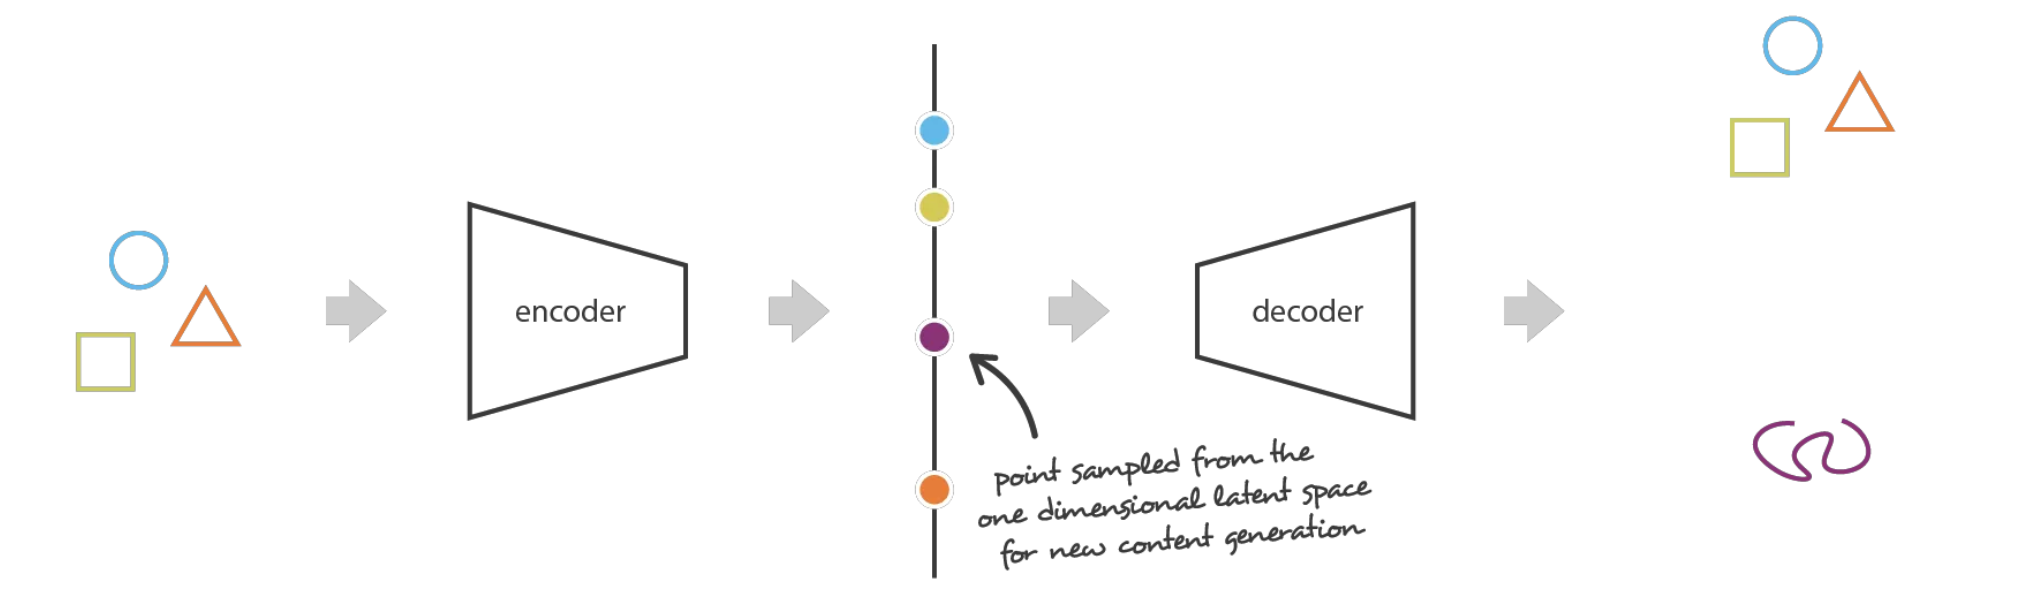
\includegraphics[width=\textwidth]{figure/EncLimit.png}
\caption{Distribuzione irregolare nello spazio latente: regioni inutilizzate o contenenti rumore}
\label{fig:enclimit}
\end{figure}

L’encoder può infatti mappare gli input in regioni isolate del latent space, lasciando vaste aree vuote. Ciò implica che, campionando casualmente un punto in questo spazio, è probabile ottenere un output privo di significato. Inoltre, non vi è garanzia che interpolazioni lineari tra due punti "validi" generino anch’esse esempi coerenti.

\section{Variational Autoencoder (VAE)}

Il \textbf{Variational Autoencoder} (VAE) è un’estensione probabilistica dell’autoencoder classico. Esso introduce una regolarizzazione nello spazio latente per consentire una generazione di dati coerente e continua. A differenza degli autoencoder tradizionali, i VAE non codificano l’input come un singolo punto nello spazio latente, ma come una distribuzione di probabilità. Il processo di training coinvolge i seguenti passaggi:

\begin{enumerate}
\item L’encoder mappa l’input in una distribuzione probabilistica (tipicamente gaussiana);
\item Viene campionato un punto da questa distribuzione;
\item Il decoder ricostruisce l’input a partire da tale punto;
\item L’errore di ricostruzione viene propagato all’indietro.
\end{enumerate}

La funzione di perdita del VAE combina due componenti, uno è il termine di ricostruzione che penalizza la differenza tra input e output, l'altro è un termine di regolarizzazione, la divergenza di Kullback-Leibler tra la distribuzione appresa e una distribuzione normale standard.

\begin{equation}\begin{split}
\mathcal{L} = \| x - \hat{x}\|^2 + \operatorname{KL}[\mathcal{N}(\mu_x,\sigma_x), \mathcal{N}(0,\operatorname{I})] =\\= \|x-\operatorname{d}(z)\|^2 + \operatorname{KL}[\mathcal{N}(\mu_x,\sigma_x), \mathcal{N}(0, \operatorname{I})]
\end{split}
\end{equation}

\subsection{Proprietà desiderate dello spazio latente}

Un buon spazio latente per la generazione di dati deve soddisfare le seguenti proprietà:

\begin{itemize}
\item \textbf{Continuità}: Piccole variazioni nel latent space devono produrre output simili;
\item \textbf{Completezza}: Qualsiasi punto dello spazio latente dovrebbe decodificarsi in un output plausibile.
\end{itemize}

Tali proprietà non sono garantite automaticamente. Le difficoltà principali includono:

\begin{itemize}
\item Encoding inadeguato: distribuzioni malformate o disgiunte non assicurano continuità o completezza.
\item Mancata regolarizzazione: il VAE può comportarsi come un autoencoder classico.
\item Distribuzioni con varianza trascurabile: rendono l’encoding troppo deterministico.
\item È necessaria una regolarizzazione sia della media che della covarianza.
\end{itemize}

\begin{figure}[!ht]
\centering
\includegraphics[width=\textwidth]{figure/RegEnc.png}
\caption{Effetti della regolarizzazione nello spazio latente}
\label{fig:regEnc}
\end{figure}

\section{Visione probabilistica dei VAE}

Consideriamo $x$ un input e $z$ una variabile latente. L’obiettivo del VAE è apprendere un modello generativo che consenta di generare nuovi campioni $x$ campionando da una distribuzione a priori su $z$, tipicamente $\mathcal{N}(0, I)$. La generazione avviene tramite:

\begin{itemize}
\item Campionamento di $z \sim p(z)$;
\item Campionamento di $x \sim p(x|z)$.
\end{itemize}

La distribuzione $p(x|z)$ è il \textit{decoder probabilistico}, mentre $p(z|x)$ è l'\textit{encoder probabilistico}. Quest’ultima risulta spesso intrattabile poiché implica il calcolo dell’integrale di marginalizzazione:

\begin{equation}
p(z|x) = \frac{p(x|z),p(z)}{p(x)} \quad,\quad p(x) = \int p(x|z),p(z),dz
\end{equation}

\subsection{Inferenza variazionale}

Per affrontare questa difficoltà, si ricorre all’\textbf{inferenza variazionale}, approssimando $p(z|x)$ con una distribuzione $q_x(z)$ scelta all’interno di una famiglia parametrica (es. gaussiana). La media e la varianza di $q_x(z)$ vengono apprese tramite funzioni $g(x)$ e $h(x)$:

\begin{equation}
\max_{(f,g,h)} \left( \mathbb{E}_{z\sim q_x}\left[-\frac{|x - f(z)|^2}{2c}\right] - \operatorname{KL}(q_x(z),|,p(z)) \right)
\end{equation}

L’obiettivo è minimizzare la distanza tra $q_x(z)$ e $p(z)$, garantendo al contempo una buona ricostruzione dell’input.

\subsection{Reparametrization Trick}

Il campionamento da $q_x(z) = \mathcal{N}(\mu_x, \sigma_x)$ non è differenziabile, impedendo l’uso diretto della backpropagation. Il \textbf{reparametrization trick} risolve questo problema: si campiona un vettore $\zeta \sim \mathcal{N}(0,I)$ e si imposta $z = \mu_x + \sigma_x \cdot \zeta$. In questo modo, il campionamento diventa un'operazione differenziabile.

\begin{figure}[!ht]
\centering
\includegraphics[width=\textwidth]{figure/RepTrick.png}
\caption{Effetto del reparametrization trick nel rendere il campionamento differenziabile}
\label{fig:repTrick}
\end{figure}

\chapter{Generative Adversarial Networks}

Le \textbf{Generative Adversarial Networks} (GAN), introdotte da \textit{Ian Goodfellow} nel 2014~\cite{goodfellow2014generative}, rappresentano una delle nuove idee nel campo dell’Intelligenza Artificiale. Si tratta di una classe di reti neurali progettate per generare dati nuovi e realistici, a partire da esempi osservati. Alla base della generazione di dati realistici c’è sempre un processo di trasformazione di semplici variabili casuali (spesso uniformi) in variabili complesse. Nonostante i calcolatori siano sistemi \textbf{deterministici} (dato un input, producono sempre lo stesso output), è comunque possibile costruire algoritmi capaci di generare sequenze numeriche che si comportano similmente a sequenze casuali. Questi algoritmi, detti \textbf{Pseudo-Random Generators}, permettono di produrre numeri che approssimano una distribuzione uniforme sull’intervallo $[0,1]$. A partire da questa base, esistono diverse tecniche per ottenere variabili casuali con distribuzioni sempre più sofisticate. Tutti questi metodi sfruttano "trucchi" matematici diversi, ma condividono un'idea comune: ottenere variabili casuali complesse come risultato di una trasformazione applicata a variabili semplici.

\section{La Trasformazione Inversa}

Una tecnica semplice è il metodo della trasformazione inversa. Supponiamo di voler generare una variabile casuale $X$ che segua una distribuzione con funzione di distribuzione cumulativa $F_X(x)$. L’idea è partire da una variabile casuale $u$ distribuita uniformemente in $\mathcal{U}(0,1)$, e ottenere $x$ tramite:
\begin{equation}
    x = F_X^{-1}(u)
\end{equation}
In questo modo, $x$ sarà distribuito secondo la legge desiderata. L’idea si può estendere anche a funzioni di trasformazione generali, che mappano variabili semplici (non necessariamente uniformi) in variabili con una distribuzione target.

\begin{figure}
    \centering
    \includegraphics[width=\textwidth]{figure/InvTrasf.png}
    \caption{In blu, la distribuzione uniforme su $[0,1]$; in arancione, una distribuzione gaussiana standard; in grigio, le linee che mostrano la mappatura dalla distribuzione uniforme a quella gaussiana.}
    \label{fig:invTrasf}
\end{figure}

\section{Modelli Generativi}

Se volessimo generare immagini in bianco e nero di cani, con dimensione $n \times n$ pixel. Ogni immagine può essere "linearizzata" in un vettore $N$ di lunghezza $n^2$, mettendo le colonne una sopra l’altra. In questo modo, ogni immagine può essere rappresentata da un punto nello spazio vettoriale $\mathbb{R}^N$. Ma attenzione: non tutti i vettori in $\mathbb{R}^N$ rappresentano cani. Solo una piccola regione di questo spazio contiene vettori che corrispondono a immagini di cani, possiamo allora immaginare l’esistenza di una distribuzione di probabilità su $\mathbb{R}^N$, che chiameremo "distribuzione dei cani", la quale assegna alta probabilità ai vettori che rappresentano immagini realistiche di cani, e probabilità molto bassa a tutto il resto. Generare un'immagine realistica significa campionare da questa "distribuzione dei cani". Tuttavia, questo ci pone di fronte a due sfide:
\begin{itemize}
    \item La distribuzione è molto complessa e vive in uno spazio ad altissima dimensione;
    \item Anche se possiamo osservarne alcuni campioni (cioè immagini vere), non sappiamo come descriverla formalmente con una formula.
\end{itemize}

Poiché non possiamo scrivere esplicitamente la distribuzione, possiamo invece lavorare sui campioni: confrontiamo immagini vere e immagini generate, e ottimizziamo il nostro modello per fare in modo che le seconde somiglino sempre di più alle prime. Questo porta a una procedura di addestramento tipica dei modelli generativi, che segue i seguenti passi:

\begin{enumerate}
    \item Generare input casuali da una distribuzione semplice (es. uniforme);
    \item Passare questi input attraverso una rete neurale generativa;
    \item Confrontare i campioni generati con quelli reali;
    \item Usare la retropropagazione per migliorare il modello e ridurre la distanza tra le due distribuzioni.
\end{enumerate}

\section{GAN}

Le \textbf{GAN} sono una potente architettura generativa che adotta una strategia diversa: invece di confrontare direttamente le distribuzioni, il modello impara attraverso un compito indiretto. In particolare, due reti neurali vengono addestrate in competizione tra loro, dette generatore e discriminatore:

\begin{itemize}
    \item Il \textbf{Generatore} cerca di produrre dati così realistici da ingannare il discriminatore;
    \item Il \textbf{Discriminatore} cerca di distinguere i dati reali da quelli generati.
\end{itemize}

Il generatore migliora cercando di ingannare sempre meglio il discriminatore, mentre il discriminatore affina le sue capacità per non farsi ingannare. Questo processo competitivo spinge entrambi i modelli a migliorare continuamente.

\subsection{Metodo diretto}

Nel metodo diretto, se conoscessimo esplicitamente la distribuzione da cui vogliamo generare i dati (per esempio una Gaussiana), potremmo confrontare la distribuzione generata con quella vera e aggiornare il generatore per ridurre la differenza. Tuttavia, come già detto, nel caso di dati complessi, come le immagini, non conosciamo la distribuzione reale in modo esplicito, pertanto questo approccio non risulta praticabile.

\subsection{Metodo indiretto}

Nel metodo indiretto, si introduce un discriminatore che ha il compito di classificare i dati come veri o falsi. Se la distribuzione dei dati generati è molto diversa da quella reale, il discriminatore li distinguerà facilmente. Quando invece le due distribuzioni iniziano a sovrapporsi, il discriminatore farà sempre più fatica, e le sue previsioni si avvicineranno al 50\%. Il generatore viene quindi addestrato per \textit{"confondere"} il discriminatore, generando dati sempre più realistici. Più riesce a farlo, più significa che le due distribuzioni si stanno avvicinando.

\subsection{Visione probabilistica}

Dal punto di vista probabilistico, il generatore prende in input una variabile latente $z$ (ad esempio, un campione da una distribuzione normale) e produce un’uscita $x' = G(z)$, che dovrebbe assomigliare a un dato reale. Il discriminatore, invece, prende un dato e restituisce la probabilità che esso sia reale: $D(x) \in [0,1]$. I due modelli vengono ottimizzati in maniera congiunta, ma con obiettivi opposti:
\begin{itemize}
    \item Il generatore cerca di far sì che $D(G(z)) \approx 1$, ovvero che il discriminatore creda che l’output generato sia reale;
    \item Il discriminatore cerca di distinguere correttamente i dati veri da quelli falsi.
\end{itemize}

Matematicamente, il generatore può essere visto come un ottimizzatore che vuole massimizzare la probabilità che i suoi output vengano classificati come reali:

\begin{equation}
    \min_G \left\{ \log(1-D(G(z))\right\}\approx \max_G\left\{-\log(D(G(z))\right\}
\end{equation}

L’intero processo può essere descritto come un problema min-max, in cui il discriminatore e il generatore si sfidano:
\begin{equation}
    \min_D\max_G\left\{-E_{x\sim Data} \log D(x) - E_{x\sim Noise}\log(1-D(G(z))\right\}
\end{equation}

Questa formulazione rappresenta il cuore delle GAN: uno sport con due giocatori che si allenano fra loro, fino a raggiungere un equilibrio in cui il generatore produce dati indistinguibili da quelli reali.
\chapter{Transformer}\label{cap:14}

I \textbf{Transformer} sono un'architettura di rete neurale introdotta nel paper \textit{"Attention Is All You Need", Vaswani et al., 2017}~\cite{vaswani2017attention}, già citato in questa serie di appunti. Essa è diventata lo standard per poter affrontare problemi relativi alle sequenze, come la traduzione automatica, linguistica o ancora problemi di visione artificiale, tutto questo grazie alla sua efficienza e capcaità di modellare realzioni a lungo termine. I Transformer si basano quasi esclusivamente su meccanismi di attenzione, elminando l'utilizzo tradizionale di reti convoluzionali o ricorrenze.

\begin{figure}
    \centering
    \includegraphics[width=0.55\textwidth]{figure/TransformerArch.png}
    \caption{La struttura Encoder-Decoder dell'architettura di un Transformer}
    \label{fig:tranArch}
\end{figure}

\section{Problemi con RNN e CNN}
Nei capitoli precedenti analizzando le reti convoluzionali e le reti ricorrenti, abbiamo notato come riscontrassero delle criticità:
\begin{itemize}
    \item \textbf{RNN}: processando i dati sequenzialmente, la difficoltà maggiore era parallelizzare i processi, un altro problema era quello relativo alla scomparsa/esplosione del gradiente su delle sequenze eccessivamente lunghe;
    \item \textbf{CNN}: queste reti neurali sono ottime per modelli locali, come per le immagini,  diventavano tuttavia molto inefficienti nel momento in cui si vuole catturare dipendenze molto lunghe, con la necessità pertanto di aumentarne la profondità.
\end{itemize}

Una delle soluzioni proposte è stata quella di usare il meccanismo dell'attenzione per modellare direttamente tutte le dipendenze in una singola sequenza, a prescindere dalla distanza, questa implementazione la ritroviamo nei Transformer.

\section{Visione ad alto livello}
Ci soffermeremo principalmente su un'applicazione dei Transformer, quella relativa alla traduzione automatica, un Transformer infatti, è in grado di prendere una frase in una lingua e generarne la traduzione in un'altra. A livello architetturale invece i Transformer si suddividono in due componenti principali:
\begin{itemize}
    \item \textbf{Encoder}: una pila di \textbf{N encoder} identici, nel paper in cui vengono presentati i Transformer ce ne sono 6, ognuno composto da due sottolivelli principali;
    \item \textbf{Decoder}: una pila di \textbf{N decoder} identici, anche in questo caso nel paper ce ne sono 6 specificando come il loro numero è strettamente collegato a quello degli encoder, anche i decoder, come gli encoder vengono strutturati in più sottolivelli.
\end{itemize}

Queste due componenti non condividono i pesi fra loro, analiziamo ora però i sottostrati degli Encoder, che sono fra loro indipendenti:

\begin{enumerate}
    \item \textbf{Self-Attention Layer}: consente all'encoder di "guardare" gli altri token presenti nella frase presa in input mentre ne elabora uno specifico per la parola presa in analisi;
    \item \textbf{Feed-Forward Neural Network}: l'output del self attention layer, viene passato a questo layer il quale applica indipendentemente le sue modifiche a ciascuna posizione del token di una frase.
\end{enumerate}

Il decoder, include gli stessi due livelli presenti nell'encoder, e ne aggiunge uno ulteriore fra i due, chiamato \textbf{Encoder-Decoder Attention}, il quale si sofferma sulle parti più rilevanti della frase mandata in input.

\begin{figure}
    \centering
    \includegraphics[width=\textwidth]{figure/EncDecTransformers}
    \caption{Rappresentazione ad alto livello di un'architettura di un Transformer, focalizzandosi principalmente sulla parte in cui vi sono gli Encoder e i Decoder}
    \label{fig:EncDecTrasf}
\end{figure}

\section{Introduzione ai Tensori}

Ogni parola data come input viene trasformata in un vettore di dimensione 512, tramite l'utilizzo di un algoritmo di embedding. L'embedding avviene solo nel primo encoder, mentre gli encoder successivi ricevono come input gli output del layer sottostante. La lunghezza della frase, dunque il numero di vettori è un \textit{iperparametro}, il quale può essere impostato durante la progettazione. Una volta effettuato l'embedding delle nostre parole, esse scorreranno all'interno dei vari layer presenti nei nostri encoder. Ogni parola segue un suo percorso indipendente all'interno dell'encoder, inoltre vengono create delle relazioni fra questi percorsi tramite il meccanismo dell'attenzione, mentre nel layer di feed-forward, non ci sono dipendenze e ciò permette l'esecuzione parallela, aumentando l'efficienza.

\section{Self-Attention}

Come già accennato in precedenza adesso, entriamo nel dettaglio per approfondire il così detto \textit{meccanismo dell'attenzione}, questo meccanismo è l'effettiva rivoluzione che viene proposta nel paper precedentemente citato, permettendo a ogni parola di ponderare la rilevanza della altre parole in una frase. Prendiamo in considerazione una frase in cui vi è un soggetto sottointesto, per noi umani risulta molto semplice determinarne chi è il soggetto, diversamente per una macchina questo risulta un meccanismo arduo. Se ci fosse un qualcosa, che permette di mettere in relazione i vari token presenti in una frase, e riuscire a determinarne le relazioni capendo effettivamente il soggetto della frase aiuterebbe molto. Infatti il \textit{self-attention mechanism}, fa proprio ciò, mettendo in relazione i singoli token e arginando questa difficoltà.

\begin{figure}
    \centering
    \includegraphics[width=0.65\textwidth]{figure/selfAttention}
    \caption{Nell'immagine possiamo vedere le singole relazioni, rappresentate dalle linee di connessione della parola \textit{it} con le altre parole della frase, più spessa è la linea, più solida riuslta essere la relazione.}
    \label{fig:selfAtt}
\end{figure}


\subsection{Self-Attention in dettaglio}

La prima fase per il calcolo della self-attention consiste nel creare ben tre vettori a partire da ogni vettore mandato in input agli encoder, nel nostro caso non sarebbero altro che gli embedding delle singole parole. Dunque vengono generati un vettore detto Query (Q), un vettore detto Key (K) e infine un vettore detto Value (V). La Self-Attention, si basa su una semplice idea: 
\begin{quote}
    Ogni parola (Query) cerca "parole chiavi" (Key), tra tutte le parole per capire da chi e quanta informazione prendere (Value).
\end{quote}

Ogni token ha un Embedding, tutti questi vengono racchiusi in un vettore degli Embedding $E$, il quale viene moltiplicato per tre matici differenti: $W^Q$, $W^K$, $W^V$, tre matrici apprese durante il training, inizialmente inizializzate a valori piccoli le quali ci permettono di ottenere rispettivamente il Query vecotr, il Key vector e il Value vector.

\begin{equation}
    Q = E \times W^Q\,,\qquad K=E\times W^K\,,\qquad V=E\times W^V
\end{equation}

Una volta calcolati i tre vettori, non facciamo altro che effettuare dei confronti, in primis calcoliamo l'affinità fra ogni $Q$ con tutte le $K$, successivamente dividiamo per la radice quadrata del valore della dimensione di $Q$ e $K$, applichiamo la funzione $\operatorname{softmax}$ che ci dirà quanto sono compatibili, e infine moltiplichiamo tutto ciò con i valori $V$, in modo tale che il token corrente mixa informazioni dagli altri token in base all'attenzione.

\begin{equation}
    \operatorname{Attention}(Q,K,V) = \operatorname{softmax}\left(\frac{Q\,K^T}{\sqrt{d_k}}\right)\,V 
\end{equation}


\subsubsection{Esempio di calcolo}
Adesso prendiamo in analisi un esempio di calcolo prendendo in considerazione di partire dalla seguente frase:
\begin{quote}
    Il gatto dorme.
\end{quote}

Ogni parola avrà un embedding corrispondente, immaginiamo in questo caso dei numeri molto semplici per facilità di comprensione:

\begin{table}[h!]
    \centering
    \caption{Embedding vettoriali delle parole}
    \begin{tabular}{@{}lc@{}}
        \toprule
        \textbf{Parola} & \textbf{Embedding} \\
        \midrule
        Il     & $\left[1, 0\right]$ \\
        Gatto  & $\left[0, 1\right]$ \\
        Dorme  & $\left[1, 1\right]$ \\
        \bottomrule
    \end{tabular}
\end{table}

Supponiamo che le nostre matrici siano delle matrici semplici, delle matrici identità o piccole trasformazioni, in modo tale che il prodotto fra matrici non sia eccessivamente complicato, nel nostro caso consideriamo che siano tutte matrici identità. Pertanto ottenendo i valori per ogni singola parola $Q,K,V$ saranno tutti la copia della singola parola presa in considerazione. Passo al confronto fra le singole parole, effettuando il prodotto scalare fra il vettore $Q$ e il vettore $K$ :

\begin{table}[h!]
    \centering
    \caption{Prodotti scalari tra Query e Key per ogni coppia di parole}
    \begin{tabular}{@{}lccc@{}}
        \toprule
        \textbf{Da} & \textbf{Il ($[1, 0]$)} & \textbf{Gatto ($[0, 1]$)} & \textbf{Dorme ($[1, 1]$)} \\
        \midrule
        Il ($Q = [1, 0]$)     & 1 & 0 & 1 \\
        Gatto ($Q = [0, 1]$)  & 0 & 1 & 1 \\
        Dorme ($Q = [1, 1]$)  & 1 & 1 & 2 \\
        \bottomrule
    \end{tabular}
\end{table}


Effettuati questi prodotti scalari, dividerò i singoli valori per la radice quadrata della grandezza dei vettori, nel nostro caso per $\sqrt{2}$ e li immetto all'interno di una \textbf{softmax}, la quale ci darà dei pesi che sommati ci porteranno a un valore unitario. Essa enfatizzerà l'importanza delle parole più rilevanti, rendendo il modello capace di contestualizzare correttamente ogni termine.

\subsubsection{L'analogia delle cartelle}
Supponiamo di avere un armadietto, al quale interno ci sono numerose cartelle, il nostro obbiettivo è trovare la cartella corrispondente al post-it che abbiamo in mano (Figura~\ref{fig:folderAn}). Il post-it in questo caso non è altro che la nostra query, le key non sono altro che l'identificativo della nostra cartella, dunque il loro nome. Una volta che trovo una corrispondenza fra la cartella e il nostro post-it, prendiamo la cartella e la poniamo al di fuori del nostro armadietto e aprendola al suo interno ci troviamo qualcosa, la quale rappresenta il value. Moltiplicare il vettore query per ogni vettore chiave produce un punteggio per ogni cartella, il quale punteggio maggiore mette in evidenza la corrispondenza più quotata fra le due parole.

\begin{figure}
    \centering
    \includegraphics[width=0.75\textwidth]{figure/FoldeAnalogy.png}
    \caption{Rappresentazione dell'analogia delle cartelle, nel quale si rappresentano i tre vettori, query vector come il post-it, key vector come l'identificativo di ogni cartella, value vector come il valore all'interno di ogni cartella, ogni cartella ha un punteggio che mappa la percentuale di corrispondenza.}
    \label{fig:folderAn}
\end{figure}

\section{Multi-Head Attention}

Il meccanismo di self-attention può essere ulteriormente potenziato tramite l'introduzione della \textbf{Multi-Head Attention}, una tecnica che migliora l'efficacia dell'attenzione secondo due principali direttrici:

\begin{enumerate}
\item Amplia la capacità del modello di focalizzarsi su posizioni differenti nella sequenza di input. Ad esempio, il vettore $z_1$ associato alla prima parola potrebbe rappresentare un misto di tutte le codifiche, ma al contempo essere fortemente influenzato dalla parola stessa;
\item Introduce molteplici \emph{sottospazi di rappresentazione} all'interno dello stesso livello di attenzione. Invece di utilizzare un singolo insieme di matrici di peso per $Q$, $K$ e $V$, si impiegano più insiemi distinti, ciascuno inizializzato in modo indipendente. Al termine dell’addestramento, ogni insieme proietta gli embedding d’ingresso in uno spazio latente diverso, catturando così vari aspetti delle relazioni tra parole.
\end{enumerate}

Questo meccanismo introduce diverse \emph{teste di attenzione} (\emph{heads}), ognuna delle quali applica il calcolo di attenzione in modo indipendente, utilizzando parametri distinti. Ogni testa analizza l’input da una prospettiva differente, permettendo al modello di cogliere vari tipi di relazioni semantiche e sintattiche tra le parole. Alla fine, i vettori prodotti da ciascuna testa ($z_i$) vengono concatenati e successivamente proiettati in uno spazio comune tramite una matrice di pesi addizionale, $W_o$, appresa durante l’addestramento. Questo passaggio ha lo scopo di restituire un singolo vettore di output da fornire al livello feed-forward della rete.

\subsubsection{Esempio}

Consideriamo nuovamente una frase semplice per illustrare il funzionamento:

\begin{quote}
Il gatto che inseguiva il topo miagolava.
\end{quote}

Focalizziamoci sulla parola \textit{miagolava}. Essa intrattiene relazioni diverse con le parole precedenti: \textit{gatto} è il soggetto che compie l’azione, \textit{inseguiva} rappresenta un’azione precedente, mentre \textit{topo} non ha relazione semantica diretta con l’azione del miagolare. Una singola testa di attenzione faticherebbe a modellare contemporaneamente tutte queste relazioni. La Multi-Head Attention risolve questo problema distribuendo l’analisi su più teste: ciascuna può concentrarsi su un tipo specifico di relazione. Alcune teste potrebbero enfatizzare il legame semantico tra soggetto e verbo, altre potrebbero evidenziare correlazioni sintattiche o ignorare completamente parole irrilevanti. Dal punto di vista grafico, ciò rende la rappresentazione visiva del meccanismo più complessa rispetto al caso della self-attention classica (Figura~\ref{fig:selfAtt}), ma allo stesso tempo più espressiva e potente (Figura~\ref{fig:multiHeadAtt}).

\begin{figure}
    \centering
    \includegraphics[width=0.5\textwidth]{figure/MultiHeadAttention}
    \caption{Esempio visivo della Multi-Head Attention: ogni testa stabilisce relazioni differenti tra la parola "it" e le altre nel contesto, evidenziate con colori distinti.}
    \label{fig:multiHeadAtt}
\end{figure}

\section{Positional Encoding}

Una limitazione intrinseca del meccanismo di self-attention è la mancanza di una nozione esplicita di ordine all'interno della sequenza. A differenza delle reti ricorrenti, i Transformer processano gli input in parallelo, senza tenere conto, di per sé, della posizione delle parole nella frase. Per colmare questa lacuna, il modello introduce un meccanismo chiamato \textbf{Positional Encoding}. Esso consiste nell’aggiunta, ad ogni embedding di input, di un vettore che codifica la posizione della parola nella sequenza. In questo modo, si conferisce al modello un senso dell’ordine, fondamentale per comprendere la struttura linguistica. I vettori di positional encoding non sono appresi durante l'addestramento, bensì definiti in modo deterministico secondo un pattern sinusoidale. La loro struttura è tale da garantire che, dopo la proiezione nei vettori $Q$, $K$ e $V$, le posizioni relative tra parole risultino distinguibili anche nel prodotto scalare dell'attenzione. In particolare, i vettori vengono definiti dalle seguenti funzioni:

\begin{equation}
    PE_{(\operatorname{pos},,2i)} = \sin\left(\frac{\operatorname{pos}}{10000^{\frac{2i}{d_{\operatorname{model}}}}}\right), \quad
    PE_{(\operatorname{pos},,2i+1)} = \cos\left(\frac{\operatorname{pos}}{10000^{\frac{2i}{d_{\operatorname{model}}}}}\right)
\end{equation}

Qui $\operatorname{pos}$ rappresenta la posizione della parola nella sequenza, $i$ è l'indice della dimensione dell'embedding, e $d_{\operatorname{model}}$ indica la dimensione totale del vettore. Ogni dimensione dell’embedding segue quindi un’onda sinusoidale con frequenza diversa, che cresce in progressione geometrica da $2\pi$ fino a $1000 \cdot 2\pi$. Questa scelta progettuale è motivata dall’intuizione che le posizioni relative tra parole possano essere modellate in modo lineare. Infatti, dato un offset $k$, il positional encoding associato alla posizione $\operatorname{pos} + k$ può essere espresso come una funzione lineare del positional encoding di $\operatorname{pos}$, facilitando il compito del modello nel cogliere le distanze relative tra parole.
\begin{figure}[hbtp]
    \centering
    \includegraphics[width=0.85\textwidth]{figure/PositionalEncoding}
    \caption{Esempio di Positional Encoding per embedding a 4 dimensioni. Ogni curva corrisponde a una dimensione del vettore.}
    \label{fig:posEncoding}
\end{figure}
Esperimenti condotti nel lavoro originale hanno dimostrato che queste funzioni sinusoidali risultano efficaci almeno quanto i positional encoding appresi, ma presentano il vantaggio di non introdurre ulteriori parametri nel modello.

\section{Residual Connections}

Nel contesto dell’architettura Transformer, le \textbf{connessioni residue} (o \textit{residual connections}) svolgono un ruolo cruciale nell’agevolare l’addestramento di reti neurali profonde e nel garantire una maggiore stabilità numerica durante la propagazione del segnale. Una connessione residua è un meccanismo architetturale che permette di sommare direttamente l’input $x$ di uno strato con il suo output trasformato $F(x)$. Formalmente, l’output risultante è dato da:

\begin{equation}
    \operatorname{Output} = F(x) + x
\end{equation}

Tale strategia è stata introdotta originariamente nelle reti ResNet, e successivamente adottata nei Transformer per i benefici che comporta in termini di stabilità e capacità di apprendimento. Essa consente al flusso informativo di "saltare" uno o più livelli, riducendo così il rischio che le trasformazioni applicate lungo la rete degradino l’informazione iniziale. Nel Transformer, ciascun blocco (sia dell’encoder che del decoder) include due moduli principali: il meccanismo di \textit{Multi-Head Attention} e il sottoblocco \textit{Feed-Forward}. Entrambi questi moduli sono avvolti da una struttura chiamata \textbf{Add \& Norm}, composta da una connessione residua e da una successiva normalizzazione (tipicamente, \textit{Layer Normalization}). In questa struttura, l’input originale viene sommato all’output del modulo, e il risultato viene poi normalizzato. Questo schema è illustrato in Figura~\ref{fig:ResAddon}.
\begin{figure}
    \centering
    \includegraphics[width=0.6\textwidth]{figure/ResidualAddon.png}
    \caption{Struttura del blocco Add \& Norm, che incapsula un modulo con connessione residua e normalizzazione.}
    \label{fig:ResAddon}
\end{figure}
L’integrazione delle connessioni residue all’interno del modello comporta numerosi vantaggi:
\begin{itemize}
    \item \textbf{Mitigazione del problema del gradiente che scompare}: facilitano la retropropagazione del gradiente anche in reti molto profonde, migliorando la stabilità dell’addestramento;
    \item \textbf{Preservazione dell’informazione originale}: permettono di conservare componenti essenziali dell’input che potrebbero essere alterate dalle trasformazioni non lineari successive;
    \item \textbf{Facilitazione dell’apprendimento}: rendono più agevole l’apprendimento di funzioni identitarie o prossime all’identità, accelerando la convergenza durante l’ottimizzazione.
\end{itemize}
Possiamo interpretare le connessioni residue come delle vere e proprie "corsie preferenziali" per il flusso informativo: il modello può scegliere se utilizzare l’informazione trasformata, conservarla intatta, o combinare entrambe. Questo è particolarmente utile in presenza di molteplici strati successivi, dove l’accumulo di trasformazioni può facilmente portare a una perdita di contenuto semantico rilevante.

\section{Decoder}

Il \textbf{decoder} ha il compito di generare la sequenza di output a partire dalla rappresentazione codificata dell’input fornita dall’encoder. In particolare, l’output dell’ultimo strato dello stack degli encoder viene trasformato in un insieme di vettori chiave ($K$) e valore ($V$), che saranno utilizzati in ogni strato del decoder all’interno del modulo \textit{Encoder-Decoder Attention}. Questo meccanismo permette al decoder di concentrarsi selettivamente su specifiche porzioni della sequenza di input, fornendo così una forma di allineamento tra input e output. Il processo si ripete iterativamente finché non viene generato un simbolo speciale di fine sequenza (\texttt{<eos>}), che segnala al modello il termine della generazione. Ad ogni passo, l’output prodotto dal decoder viene reinserito come input per il passo successivo, e tale operazione prosegue lungo la pila di decoder in maniera analoga a quanto accade per l’encoder. Anche nel decoder, viene incorporata l’informazione posizionale, attraverso apposite rappresentazioni, per permettere al modello di distinguere l’ordine delle parole nella sequenza.
\begin{figure}
    \centering
    \includegraphics[width=\textwidth]{figure/DecoderSample.png}
    \caption{Esempio del processo di generazione nel decoder al secondo step temporale. Nel primo step è stata generata la parola \textit{I} come traduzione di \textit{je}.}
    \label{fig:DecSam}
\end{figure}
Una differenza sostanziale rispetto al funzionamento dell’encoder risiede nel meccanismo di \textbf{self-attention} impiegato nel decoder. In questo caso, l’attenzione è \textit{mascherata} per evitare che il modello acceda a posizioni future della sequenza di output. Più precisamente, le posizioni successive a quella corrente vengono oscurate (mascherate) assegnando loro un valore $-\infty$ prima dell'applicazione della funzione $\operatorname{softmax}$, così da annullarne il contributo. Il modulo \textit{Encoder-Decoder Attention}, invece, opera in maniera analoga alla self-attention multi-testa, con la differenza che le matrici $K$ e $V$ provengono direttamente dall’output dello stack degli encoder, mentre le matrici $Q$ (Query) vengono calcolate a partire dallo strato sottostante del decoder stesso.

\subsection{Final Layer e Softmax}

Lo stack dei decoder, al termine della generazione, produce un vettore continuo (un vettore di float), che deve essere convertito in una parola del vocabolario. A questo scopo intervengono due componenti finali: il \textbf{Final Linear Layer} e il \textbf{Softmax Layer}. Il \textit{Final Linear Layer} è una rete completamente connessa che trasforma il vettore di rappresentazione generato dal decoder in un \textbf{vettore di logit}, detto anche \textit{logits vector}. Questo vettore ha una dimensione pari alla cardinalità del vocabolario: ad esempio, se il modello gestisce un vocabolario di 10.000 parole, il vettore sarà lungo 10.000, e ciascun valore rappresenterà il punteggio non normalizzato associato a una specifica parola. Il \textit{Softmax Layer} converte questo vettore di logit in una distribuzione di probabilità: tutti i valori risultanti saranno positivi e la loro somma sarà pari a uno. L’indice con la probabilità più alta indicherà la parola da generare in quello specifico time step.

\begin{figure}
    \centering
    \includegraphics[width=0.75\textwidth]{figure/FinalLayer.png}
    \caption{Struttura dei layer finali del decoder nel Transformer, che trasformano la rappresentazione vettoriale in una parola.}
    \label{fig:FinLay}
\end{figure}

\section{Allenamento di un Transformer}

Durante la fase di \textbf{addestramento}, il Transformer esegue un \textit{forward pass} sui dati forniti. Poiché il dataset di training è etichettato, è possibile confrontare le uscite del modello con i target attesi, valutando così la qualità delle predizioni. In presenza di discrepanze tra output previsto e desiderato, si procede con un aggiornamento dei pesi tramite backpropagation, al fine di minimizzare l’errore e migliorare la capacità predittiva del modello. I vocabolari utilizzati nei Transformer contengono generalmente un numero elevato di parole, oltre a simboli speciali come \texttt{<eos>} (\textit{end of sequence}), che indica al modello il termine della sequenza da generare. Prima dell’allenamento, ogni parola viene mappata su un vettore numerico tramite un processo di \textit{preprocessing}. Una rappresentazione comune è la \textbf{One-Hot Encoding}, in cui ogni parola è rappresentata da un vettore con tutti zeri, tranne un valore pari a uno in corrispondenza della posizione associata alla parola nel vocabolario. Nelle prime fasi di training, un modello non ancora addestrato produce uscite casuali e scorrelate dal target. L’obiettivo dell’addestramento è dunque quello di guidare il modello a produrre, per ciascun time step, una distribuzione di probabilità in cui la parola attesa abbia la probabilità più alta. Ogni distribuzione è un vettore di lunghezza pari al numero di parole nel vocabolario, e la sequenza di distribuzioni dovrebbe idealmente riflettere la sequenza di parole target. In particolare, ci si aspetta che la prima distribuzione assegni il valore di probabilità più alto alla prima parola desiderata, la seconda alla seconda parola, e così via, fino all’ultima distribuzione, in cui la probabilità più alta dovrebbe corrispondere al token \texttt{<eos>}, segnalando la fine della sequenza.

\begin{figure}
    \centering
    \includegraphics[width=0.8\textwidth]{figure/TrainExpectation}
    \caption{Distribuzioni di probabilità prodotte dal decoder: ogni posizione temporale è associata a una distribuzione su tutto il vocabolario, e ci si aspetta che la parola target sia quella con la probabilità massima.}
    \label{fig:trainExp}
\end{figure}

\section{Oltre la struttura base del Transformer}

Con la comprensione completa dell'architettura originaria del Transformer, siamo ora pronti ad analizzare alcune delle estensioni fondamentali che hanno reso questo modello uno standard de facto nel campo del deep learning. In particolare, approfondiremo come il Transformer venga adattato a contesti specifici mediante il \textbf{fine-tuning}, quali siano le sue principali \textbf{applicazioni} in scenari reali e accademici, e infine esamineremo alcune delle \textbf{varianti architetturali} che ne estendono le potenzialità, spesso superandone i limiti originali.

\section{Fine-Tuning del Transformer}

Il \textbf{fine-tuning} è una tecnica di apprendimento trasferito (\textit{transfer learning}) ampiamente adottata nel contesto dei Transformer, che consente di adattare un modello pre-addestrato a un compito specifico. Il modello viene inizialmente addestrato su un vasto corpus general-purpose (come Wikipedia o Common Crawl), apprendendo rappresentazioni linguistiche ricche e versatili. Successivamente, viene ottimizzato su un dataset mirato, spesso molto più piccolo, relativo a un task specifico (ad esempio, classificazione di sentiment, riconoscimento di entità, generazione di codice, ecc.).

Il processo si articola come segue:
    \begin{enumerate}
        \item \textbf{Pretraining}: il modello viene addestrato in maniera auto-supervisionata su un task generale (e.g. \textit{masked language modeling} o \textit{causal language modeling}).
        \item \textbf{Fine-tuning supervisionato}: si sostituisce o si estende la testa del modello con uno o più layer adatti al task target (es. classificazione), e si effettua un training supervisionato con gradient descent.
    \end{enumerate}

Uno degli aspetti cruciali del fine-tuning è la scelta del \textit{learning rate}: un tasso troppo elevato potrebbe sovrascrivere le rappresentazioni apprese nel pretraining; al contrario, uno troppo basso potrebbe non fornire l'adattamento desiderato.

\section{Applicazioni del Transformer}

L'architettura Transformer è stata adottata in una vasta gamma di applicazioni, sia in ambito linguistico che in domini non testuali. Tra le principali:

\begin{itemize}
    \item \textbf{Natural Language Processing (NLP)}: è il dominio originario del Transformer, dove viene impiegato in:
    \begin{itemize}
        \item Traduzione automatica (e.g. Google Translate)
        \item Generazione di testo (e.g. ChatGPT, GPT-4)
        \item Analisi del sentiment
        \item Estrazione di entità (NER)
        \item Riassunto automatico
    \end{itemize}
    \item \textbf{Visione artificiale (CV)}: con modelli come Vision Transformer (ViT), l'architettura viene adattata al dominio visivo per compiti come classificazione, segmentazione e object detection.\item \textbf{Bioinformatica e Chimica Computazionale}: i Transformer vengono utilizzati per la modellazione di sequenze proteiche, il drug discovery, e la predizione di interazioni molecolari.
    \item \textbf{Codice e programmazione automatica}: modelli come Codex e CodeBERT sfruttano il Transformer per comprendere e generare codice sorgente.
    \item \textbf{Musica, immagini e altre modalità}: modelli come MuseNet o DALL·E impiegano architetture Transformer per generare musica e immagini, integrando capacità multi-modali.
\end{itemize}

\section{Varianti dell'Architettura Transformer}

L'efficacia e la flessibilità del Transformer hanno portato allo sviluppo di numerose varianti architetturali, ciascuna con caratteristiche peculiari. Tra le più importanti:

\subsection{BERT (Bidirectional Encoder Representations from Transformers)}
BERT è una variante del Transformer basata esclusivamente sulla pila di encoder. Il pretraining viene effettuato tramite \textit{Masked Language Modeling} (MLM) e \textit{Next Sentence Prediction} (NSP), rendendolo particolarmente adatto per task di classificazione, QA e NER.

\subsection{GPT (Generative Pretrained Transformer)}
GPT, in particolare nelle sue versioni più recenti, utilizza esclusivamente la pila di decoder con attenzione causale. È ottimizzato per la generazione di testo autoregressiva e mostra prestazioni notevoli in numerosi task senza necessità di fine-tuning esplicito (few-shot learning).

\subsection{T5 (Text-To-Text Transfer Transformer)}
T5 propone un approccio uniforme in cui ogni task NLP è riformulato come un problema di traduzione da testo a testo, permettendo al modello di utilizzare una singola architettura per una varietà di compiti diversi, come classificazione, traduzione e completamento.

\subsection{Vision Transformer (ViT)}
ViT adatta il Transformer all’elaborazione di immagini, dividendo un’immagine in patch (simili a token testuali) e trattandole come una sequenza da processare tramite attenzione. Questa strategia ha ottenuto risultati competitivi nei benchmark di visione artificiale.

\subsection{Longformer, Performer, Linformer}
Queste varianti propongono meccanismi di attenzione ottimizzati per lunghe sequenze, affrontando il limite di complessità quadratica dell’attenzione standard, mediante sparsità, kernelizzazione o proiezioni lineari.

\begin{sidewaystable}[htbp]
    \centering
    \renewcommand{\arraystretch}{1.3}
    \caption{Confronto tra principali varianti del modello Transformer.}
    \label{tab:transformer_variants}
    \begin{tabularx}{\textwidth}{>{\bfseries}l c X X}
        \toprule
        Modello & Stack & Task Principali & Caratteristiche Peculiari \\
        \midrule
        BERT & Encoder & Classificazione, NER, QA &
        Pretraining con Masked Language Modeling (MLM) e Next Sentence Prediction (NSP). Attenzione bidirezionale. \\
        GPT & Decoder & Generazione di testo, completamento, traduzione &
        Addestramento autoregressivo (unidirezionale) tramite language modeling. \\
        T5 & Encoder-Decoder & Tutti i task NLP (in forma testo-testo) &
        Architettura unificata: ogni task è trattato come una traduzione. Buona generalizzazione. \\
        ViT & Encoder & Classificazione immagini, segmentazione &
        Applica il Transformer alla visione computazionale: utilizza patch e positional embedding. \\
        Longformer & Encoder & Elaborazione di lunghe sequenze testuali &
        Combina attenzione locale e globale per ridurre la complessità. Adatto a documenti estesi. \\
        Performer & Encoder & Elaborazione efficiente di sequenze lunghe &
        Approssima l’attenzione softmax tramite metodi kernel, riducendo la complessità a $O(n)$. \\
        Linformer & Encoder & Task sequenziali su lunghi input &
        Proietta $K$ e $V$ in spazi ridotti, ottenendo attenzione lineare. \\
        \bottomrule
    \end{tabularx}
\end{sidewaystable}


\section{BERT nel dettaglio}

\textbf{BERT} (Bidirectional Encoder Representations from Transformers) è un modello di linguaggio basato esclusivamente sulla componente Encoder dell'architettura Transformer. Proposto da Google nel 2018, è stato pre-addestrato su un ampio corpus di testi (Wikipedia e BooksCorpus), acquisendo una solida conoscenza linguistica generale. Una delle caratteristiche distintive di BERT è la sua natura \textit{bidirezionale}: il modello è in grado di analizzare simultaneamente il contesto a sinistra e a destra di una parola. Questo contrasta con i modelli precedenti, che si focalizzavano unicamente sul contesto passato (left-to-right) o futuro (right-to-left). Inoltre, BERT è \textit{contestuale}, ovvero assegna un significato a ogni parola in funzione del contesto in cui appare. Sono disponibili due versioni principali di BERT:
\begin{itemize}
    \item \textbf{BERT Base}: 12 strati Transformer, 768 unità nascoste, 12 teste di attenzione;
    \item \textbf{BERT Large}: 24 strati Transformer, 1024 unità nascoste, 16 teste di attenzione.
\end{itemize}
Entrambe le versioni utilizzano esclusivamente Encoder.

\subsection{Gestione dell'input}

\begin{enumerate}
    \item L'input testuale viene tokenizzato e successivamente trasformato in vettori di embedding;
    \item Un token speciale [CLS] viene anteposto alla sequenza, utile per i compiti di classificazione;
    \item Tra due frasi distinte viene inserito un token [SEP], che funge da delimitatore;
    \item Viene sommato un \textit{positional encoding} per preservare l'informazione sull'ordine dei token;
    \item Si aggiungono embedding di segmento per distinguere tra la frase A e la frase B;
    \item Ogni encoder layer applica un meccanismo di self-attention seguito da un feed-forward network.
\end{enumerate}

\subsection{Gestione dell'output}

\begin{enumerate}
    \item Ogni token genera un vettore di dimensione \texttt{hidden\_size} (768 nel caso di BERT base);
    \item Per i compiti di classificazione, si utilizza il vettore associato al token [CLS];
    \item Tale vettore viene poi passato a un classificatore seguito da una funzione softmax per ottenere una distribuzione di probabilità sulle classi.
\end{enumerate}

\subsection{Addestramento di BERT}

Il pretraining di BERT è risultata fondamentale per poter rendere questo modello potente e generalizzabile, giungendo a ottenere nella raccolta dati circa 3.3 miliardi di parole, esso si basa su due task principali:

\subsubsection{Masked Language Modeling (MLM)}

Il 15\% dei token viene selezionato casualmente e mascherato:
\begin{itemize}
    \item 80\% dei token selezionati viene sostituito con il token speciale [MASK];
    \item 10\% viene sostituito con un token casuale;
    \item 10\% rimane invariato.
\end{itemize}
Il modello è poi addestrato a predire il token originale, sfruttando l'intero contesto circostante.

\subsubsection{Next Sentence Prediction (NSP)}

A BERT vengono fornite coppie di frasi:
\begin{itemize}
    \item Nel 50\% dei casi, la seconda frase è effettivamente quella che segue la prima nel testo originale;
    \item Nel restante 50\%, è una frase casuale.
\end{itemize}
Questo task è pensato per insegnare al modello le relazioni semantiche tra frasi consecutive.

\subsection{Utilizzi di BERT}

BERT può essere impiegato in due principali modalità:

\begin{itemize}
    \item \textbf{Fine-tuning}: si aggiunge un classificatore in cima a BERT e si addestra l'intero modello su uno specifico task. Tutti i pesi, inclusi quelli di BERT, vengono aggiornati durante il training;
    \item \textbf{Feature extraction}: si utilizzano gli embedding contestuali generati da BERT come input per modelli esterni, sfruttando la ricca rappresentazione appresa.
\end{itemize}

\section{GPT nel dettaglio}

\textbf{GPT} (Generative Pretrained Transformer) è una famiglia di modelli linguistici autoregressivi, introdotti da OpenAI. A differenza di BERT, che si basa sull’encoder dei Transformer, GPT utilizza esclusivamente la componente \textit{decoder} dell'architettura originale (Figura~\ref{fig:GPTModel}). La versione iniziale di GPT è stata rilasciata nel 2018, seguita da GPT-2 (2019), GPT-3 (2020) e GPT-4 (2023), ciascuna caratterizzata da una scala crescente di parametri e capacità di generalizzazione.

\begin{figure}
    \centering
    \includegraphics[width=0.85\textwidth]{figure/GPTModel}
    \caption{Possiamo vedere nell'immagine le varie tipologie di modelli di GPT-2, qui vi sono a seconda della grandezza diverse dimensioni del modello, utilizzando più decoder a seconda della grandezza del modello stesso.}
    \label{fig:GPTModel}
\end{figure}

\subsection{Architettura e funzionamento}

GPT è un modello Transformer unidirezionale, ovvero genera una parola alla volta considerando solo il contesto precedente. Il principio fondamentale è l'autoregressione: il modello predice la parola successiva $x_t$ data la sequenza delle parole precedenti $(x_1, x_2, ..., x_{t-1})$.

\subsubsection{Input e Tokenizzazione}

\begin{itemize}
    \item Il testo viene tokenizzato mediante una tecnica di tipo Byte-Pair Encoding (BPE);
    \item Ogni token viene convertito in un vettore di embedding;
    \item Viene aggiunto un \textit{positional embedding} per conservare l’informazione sull’ordine dei token;
    \item A differenza di BERT, non viene inserito alcun token [CLS] o [SEP], poiché GPT non è progettato per la classificazione o il confronto fra frasi.
\end{itemize}

\subsubsection{Decoder e Self-Attention causale}

GPT utilizza unicamente blocchi decoder del Transformer. Ogni blocco è composto da:
\begin{itemize}
    \item \textbf{Masked Self-Attention}: l'attenzione è limitata ai soli token precedenti mediante una \textit{causal mask}, impedendo al modello di vedere token futuri;
    \item \textbf{Feed-forward network} applicato a ciascun token individualmente;
    \item \textbf{Layer normalization} e \textbf{residual connections}, analogamente al Transformer standard.
\end{itemize}

\subsubsection{Output e Generazione}

\begin{itemize}
    \item Il vettore finale associato all’ultimo token viene proiettato nello spazio vocabolario tramite una matrice di output;
    \item Viene applicata una softmax per ottenere una distribuzione di probabilità sulle parole successive;
    \item Il token con la probabilità più alta può essere selezionato (greedy), oppure campionato (ad es. con temperature scaling o nucleus sampling);
    \item Questo processo viene iterato per generare una sequenza coerente parola dopo parola.
\end{itemize}

\subsection{Scelta del Token successivo}
Una volta che viene effettuato tutto il processo di analisi attraversando i decoder, ciò che viene generato alla fine è un vettore in cui sono presenti diverse probabilità di preddizione relative alla parola successiva della nostra frase, per scegliere di quale parola si tratta ci sono varie modalità adottate:

\begin{itemize}
    \item\textbf{Argmax}: Scelto il token con probabilità massima;
    \item\textbf{Sampling}: Si estra un token a caso, seguendo la distribuzione di probabilità fornita;
    \item\textbf{Top-k sampling}: Si considerano solo i top-k token probabili, per poi selezionare il token fra questi;
    \item\textbf{Top-p nucleus sampling}: Vengono considerati solo i token la cui somma delle probabilità supera un valore $p$, per poi selezionare un token fra questi in maniera casuale;
    \item\textbf{Beam Search}: Vengono mantenute più sequenze candidate contemporaneamente, il costo computazionale è elevato;
\end{itemize}

\begin{Osservazione}
    L'argmax, è una specializzazione del Top-k sampling, dove il valore di k è unitario.
\end{Osservazione}

\subsection{Pretraining}

GPT viene pre-addestrato in modo non supervisionato su un ampio corpus testuale, ottimizzando la funzione di perdita cross-entropy per predire il token successivo:
\[
\mathcal{L} = -\sum_{t=1}^{T} \log P(x_t \mid x_1, ..., x_{t-1})
\]
Non vi è masking di token né predizione bidirezionale: il modello impara a generare testo in modo fluente e coerente, acquisendo conoscenza grammaticale, lessicale e semantica implicita.

\subsection{Utilizzo in downstream tasks}

GPT può essere adattato a compiti specifici in due modalità:

\begin{itemize}
    \item \textbf{Fine-tuning supervisionato}: il modello viene addestrato su dataset etichettati per compiti come classificazione, QA, traduzione, ecc. (tipico in GPT-2);
    \item \textbf{Prompt-based learning}: grazie alla sua natura generativa, GPT può essere utilizzato in modalità \textit{zero-shot}, \textit{few-shot} o \textit{one-shot}, semplicemente modificando il prompt di input per adattarsi al task desiderato (approccio introdotto con GPT-3).
\end{itemize}

\begin{table}
    \centering
    \caption{Confronto tra BERT e GPT.}
    \begin{adjustbox}{width=\textwidth}
    \begin{tabular}{|l|c|c|}
    \hline
    \textbf{Caratteristica} & \textbf{BERT} & \textbf{GPT} \\
    \hline
    Architettura & Encoder Transformer & Decoder Transformer \\
    Direzionalità & Bidirezionale & Unidirezionale (autoregressivo) \\
    Obiettivo pretraining & MLM + NSP & Language Modeling \\
    Token speciali & [CLS], [SEP], [MASK] & Nessuno \\
    Uso principale & Comprensione del linguaggio & Generazione del linguaggio \\
    Modalità di utilizzo & Fine-tuning, feature extraction & Prompting, fine-tuning \\
    \hline
    \end{tabular}
    \end{adjustbox}
\end{table}
\section*{Approfondimenti}
\section{Varianti dei modelli Transformer}

Nel corso degli anni, numerose varianti dell’architettura Transformer sono state sviluppate per migliorarne l’efficienza, la generalizzazione e l’adattabilità a specifici compiti. Di seguito si riportano alcune delle più rilevanti:

\subsection{RoBERTa (Robustly Optimized BERT Approach)}

RoBERTa è una versione migliorata di BERT, introdotta da Facebook AI, che elimina l’obiettivo NSP, utilizza una maggiore quantità di dati e addestra il modello più a lungo. Le principali modifiche includono:
\begin{itemize}
    \item Rimozione del Next Sentence Prediction (NSP);
    \item Addestramento su batch più grandi e sequenze più lunghe;
    \item Dinamica del masking modificata ad ogni epoca.
\end{itemize}
RoBERTa ha mostrato prestazioni superiori a BERT in numerosi benchmark NLP.

\subsection{ALBERT (A Lite BERT)}

ALBERT propone un modello più leggero e scalabile mediante:
\begin{itemize}
    \item Condivisione dei pesi tra i layer;
    \item Fattorizzazione della matrice di embedding;
    \item Nuovo obiettivo di pretraining: \textit{Sentence Order Prediction (SOP)}.
\end{itemize}
Queste modifiche riducono drasticamente il numero di parametri, rendendo ALBERT più efficiente senza compromettere l’accuratezza.

\subsection{GPT-2, GPT-3 e GPT-4}

Le versioni successive della famiglia GPT hanno introdotto miglioramenti principalmente attraverso la scala del modello:
\begin{itemize}
    \item \textbf{GPT-2} (2019): 1.5 miliardi di parametri, addestrato su un ampio corpus web;
    \item \textbf{GPT-3} (2020): 175 miliardi di parametri, addestrato in modo da supportare \textit{few-shot} e \textit{zero-shot learning};
    \item \textbf{GPT-4} (2023): architettura multimodale, maggiore robustezza e comprensione contestuale, con performance avanzate su molteplici benchmark.
\end{itemize}

\subsection{ChatGPT e InstructGPT}

\begin{itemize}
    \item \textbf{InstructGPT} è una versione di GPT-3 fine-tunata mediante \textit{reinforcement learning from human feedback} (RLHF) per seguire istruzioni umane;
    \item \textbf{ChatGPT} è un'applicazione conversazionale basata su InstructGPT/GPT-3.5 o GPT-4, ottimizzata per generare risposte fluide, coerenti e utili in scenari di dialogo.
\end{itemize}

\subsection{Altri modelli noti}

\begin{itemize}
    \item \textbf{DistilBERT}: versione compressa di BERT, con il 40\% di parametri in meno e il 97\% delle performance;
    \item \textbf{ELECTRA}: introduce un pretraining discriminativo invece del classico MLM;
    \item \textbf{T5 (Text-to-Text Transfer Transformer)}: unifica i compiti NLP in un’unica formulazione testuale.
\end{itemize}

\section{Applicazioni pratiche dei Transformer}

L’adattabilità dei modelli Transformer consente la loro applicazione in una vasta gamma di task di NLP, sia in modalità supervisionata (fine-tuning) che non supervisionata (prompt engineering):

\begin{itemize}
    \item \textbf{Classificazione testuale}: assegnazione di etichette a frasi, documenti, tweet, ecc. (es. analisi del sentiment);
    \item \textbf{Named Entity Recognition (NER)}: identificazione di entità rilevanti nel testo (nomi, date, organizzazioni);
    \item \textbf{Risposta a domande (QA)}: estrazione o generazione di risposte date una domanda e un contesto;
    \item \textbf{Traduzione automatica}: conversione da una lingua a un’altra (es. inglese → francese);
    \item \textbf{Generazione di testo}: produzione di frasi o paragrafi coerenti a partire da un prompt (storytelling, copywriting);
    \item \textbf{Riassunto automatico}: estrazione o generazione di versioni sintetiche di testi lunghi;
    \item \textbf{Conversational AI}: chatbot e assistenti virtuali, spesso costruiti su InstructGPT o ChatGPT;
    \item \textbf{Codice e programmazione}: generazione di codice (es. Codex), spiegazione di funzioni o completamento automatico.
\end{itemize}

\section{Evoluzione dei Transformer}

L’evoluzione dei modelli Transformer è stata caratterizzata da un rapido progresso sia in termini di architettura che di scala computazionale. Di seguito è riportata una timeline dei principali modelli:

\begin{itemize}
    \item \textbf{2017 – Transformer} \cite{vaswani2017attention}: introduzione dell’architettura self attentiva in "Attention is All You Need".
    \item \textbf{2018 – BERT} \cite{devlin2018bert}: encoder bidirezionale pre-addestrato con obiettivi MLM e NSP.
    \item \textbf{2019 – GPT-2} \cite{radford2019language}: modello autoregressivo di grandi dimensioni per generazione testuale.
    \item \textbf{2019 – RoBERTa} \cite{liu2019roberta}: ottimizzazione di BERT tramite addestramento più esteso e rimozione NSP.
    \item \textbf{2019 – DistilBERT} \cite{sanh2019distilbert}: distillazione di BERT per maggiore efficienza.
    \item \textbf{2020 – T5} \cite{raffel2020exploring}: approccio "text-to-text" per unificare i compiti NLP.
    \item \textbf{2020 – GPT-3} \cite{brown2020language}: 175 miliardi di parametri, abilità few-shot learning.
    \item \textbf{2020 – ELECTRA} \cite{clark2020electra}: discriminatore al posto di un tradizionale generatore.
    \item \textbf{2021 – InstructGPT} \cite{ouyang2022training}: RLHF per migliorare l’allineamento con le intenzioni umane.
    \item \textbf{2022 – ChatGPT}: versione ottimizzata per il dialogo basata su InstructGPT.
    \item \textbf{2023 – GPT-4}: modello multimodale con prestazioni avanzate in molti contesti.
\end{itemize}




\chapter{Diffusion Models}\label{cap:15}

In questo capitolo affrontiamo una tematica profondamente diversa da quanto visto finora: l’utilizzo dei modelli di Deep Learning per la generazione di immagini. In precedenza, abbiamo esplorato l'approccio delle \textbf{Generative Adversarial Networks} (GAN), in cui si apprende direttamente la distribuzione di probabilità da cui si desidera generare nuovi dati. Ora ci concentriamo su una nuova metodologia, oggi ampiamente diffusa: i \textbf{modelli di diffusione}. Accanto ai modelli di diffusione, è importante segnalare l’emergere di una nuova famiglia di modelli generativi sviluppati nel 2024, i quali non verranno trattati in questi appunti. I modelli di diffusione si fondano su un'intuizione tanto semplice quanto potente: corrompere progressivamente un dato (ad esempio, un'immagine) aggiungendo rumore, fino a trasformarlo in rumore puro, e poi addestrare un modello per compiere il processo inverso, ovvero rimuovere gradualmente il rumore per recuperare l’immagine originale (Figura~\ref{fig:diffMod}). L’ispirazione teorica proviene dalla termodinamica, in cui i processi stocastici descrivono il passaggio da uno stato ordinato a uno disordinato e viceversa. In questo contesto, il "rumore" rappresenta una forma di disordine che viene artificialmente introdotta e poi eliminata in maniera appresa.

\begin{figure}
    \centering
    \includegraphics[width=\textwidth]{figure/diffusionModel}
    \caption{Schema di un modello di diffusione: nel processo forward si aggiunge rumore progressivamente a un’immagine, mentre nel processo inverso (reverse diffusion) si parte dal rumore per ricostruire l’immagine originale.}
    \label{fig:diffMod}
\end{figure}

\section{Stable Diffusion}

Una delle implementazioni più rilevanti e ottimizzate dei modelli di diffusione è rappresentata dalla \textbf{Stable Diffusion}. Il suo contributo principale è l’efficienza computazionale, ottenuta spostando il processo di diffusione in uno \textit{spazio latente} compresso, piuttosto che operare direttamente sui pixel dell’immagine. Questo approccio, che ricorda quanto già discusso nei modelli autoencoder, consente di ridurre drasticamente il costo computazionale.

\section{Task dei modelli di diffusione}

Stable Diffusion consente di affrontare molteplici task generativi. Tra i più significativi vi sono:
\begin{itemize}
    \item \texttt{text2img}: generazione di immagini a partire da un prompt testuale;
    \item \texttt{text+image}: generazione o modifica di immagini a partire da un’immagine parziale e un prompt testuale (e.g., image-to-image, inpainting).
\end{itemize}

In entrambi i casi, il modello è composto da tre moduli principali:
\begin{enumerate}
    \item \textbf{Text Encoder}: converte il prompt testuale in un embedding numerico (utilizzando il modello CLIP);
    \item \textbf{Image Information Creator}: un modello U-Net, dotato di uno scheduler, che effettua il processo di denoising nello spazio latente;
    \item \textbf{Image Decoder}: decodifica lo spazio latente nell’immagine finale, tramite un Autoencoder.
\end{enumerate}

\begin{figure}
    \centering
    \includegraphics[width=\textwidth]{figure/t2imgAndtextandtext}
    \caption{A sinistra, esempio di task \texttt{text2img}; a destra, task \texttt{text+image} (image-to-image, inpainting).}
    \label{fig:stabDiff}
\end{figure}

\section{Meccanismo di diffusione}

Il processo di diffusione avviene attraverso una sequenza di step successivi. A ogni passo, il modello prende in input un vettore latente e lo aggiorna aggiungendo o rimuovendo informazioni, in funzione del task. Progressivamente, il vettore latente assume una forma sempre più coerente con l’immagine desiderata. Se si visualizzasse il risultato decodificato dopo ciascuno di questi passaggi, si otterrebbe una serie di immagini via via più definite, convergenti verso la versione finale (Figura~\ref{fig:stepDiff}).

\begin{figure}
    \centering
    \includegraphics[width=\textwidth]{figure/DiffusionStep.png}
    \caption{Output decodificato progressivamente a ogni step della diffusione inversa.}
    \label{fig:stepDiff}
\end{figure}

\section{Diffusione inversa}

Il processo inverso richiede la conoscenza del quantitativo di rumore aggiunto a un’immagine in ciascuno step. Per questo, si addestra un modello neurale — il \textbf{noise predictor} — a stimare il rumore presente in un’immagine latente. Tale modello è una rete U-Net e viene addestrato come segue:
\begin{enumerate}
    \item Si seleziona un'immagine dal dataset (es. un gatto);
    \item Si genera una quantità casuale di rumore;
    \item Si corrompe l'immagine originale sommando il rumore;
    \item Si addestra il noise predictor a stimare il rumore aggiunto.
\end{enumerate}

Una volta addestrato, il modello può essere utilizzato per il processo di \textit{denoising}: si parte da rumore puro, si stima il rumore presente e lo si sottrae iterativamente. Questo processo, ripetuto più volte, conduce alla generazione di un'immagine coerente (Figura~\ref{fig:revDiff}).
\begin{figure}
    \centering
    \includegraphics[width=\textwidth]{figure/ReverseDiffusion.png}
    \caption{Esempio di reverse diffusion: il rumore viene rimosso progressivamente fino a ottenere un’immagine pulita.}
    \label{fig:revDiff}
\end{figure}
È importante sottolineare che, in assenza di ulteriori vincoli, la generazione è \textit{incondizionata}, ovvero il contenuto dell'immagine è determinato in modo casuale.

\section{Conditioning}

Per generare immagini coerenti con un prompt testuale, è necessario condizionare il processo di diffusione. Questo avviene introducendo il testo all’interno della pipeline attraverso un \textbf{Text Encoder}, che ne produce un embedding vettoriale. Questo embedding viene poi integrato nel noise predictor tramite meccanismi di \textbf{cross-attention}, permettendo al modello di generare un contenuto visivo coerente con il linguaggio naturale.

\subsection{Cross-Attention}

Il meccanismo di \textbf{cross-attention} consente a una sequenza di essere guidata da un’altra. A differenza della \textit{self-attention}, che confronta una sequenza con sé stessa, la cross-attention confronta una sequenza (es. testo) con un’altra (es. immagine latente). Nel caso di Stable Diffusion:
\begin{itemize}
    \item Il \textbf{Text Encoder CLIP} genera un embedding del prompt;
    \item La \textbf{U-Net} utilizza sia self-attention (per coerenza interna) sia cross-attention (per coerenza col prompt);
    \item Il risultato è un’immagine generata che riflette fedelmente il contenuto testuale.
\end{itemize}

\subsubsection{CLIP}

CLIP combina un encoder per immagini e uno per testi. Durante l’addestramento, dati un’immagine e una descrizione testuale, entrambi vengono trasformati in embedding. Si massimizza poi la \textbf{cosine similarity} tra i due vettori, affinché corrispondano semanticamente. Il processo è iterato e ottimizzato tramite backpropagation.

\subsubsection{Cross-Attention nei Transformer}

Nel contesto dei Transformer, la cross-attention combina due sequenze: una da cui si calcolano le \textit{Key} e \textit{Value}, e una da cui si ottengono le \textit{Query}. Il risultato finale ha la dimensione della sequenza delle Query.
\begin{figure}
    \centering
    \includegraphics[width=0.25\textwidth]{figure/CrossTrasformer.png}
    \caption{Schema del meccanismo di cross-attention all'interno di un Transformer.}
    \label{fig:crossTrasf}
\end{figure}

\subsubsection{Algoritmo della Cross-Attention}

\begin{enumerate}
    \item Ottenere due sequenze $S_1$ (per Key e Value) e $S_2$ (per Query);
    \item Calcolare $K, V$ da $S_1$;
    \item Calcolare $Q$ da $S_2$;
    \item Calcolare la matrice di attenzione da $Q$ e $K$;
    \item Applicare la matrice di attenzione ai $V$;
    \item L’output ha dimensione pari a $S_2$.
\end{enumerate}

\begin{figure}
    \centering
    \includegraphics[width=0.7\textwidth]{figure/StableDiffusionArchitecture.png}
    \caption{Architettura completa della Stable Diffusion.}
    \label{fig:StabDiffArch}
\end{figure}

\subsubsection{Cross-Attention nel Perceiver IO}

Il \textbf{Perceiver IO} è un'architettura multimodale in grado di gestire input e output eterogenei. Utilizza la cross-attention per mescolare input multimodali in una rappresentazione latente compatta, permettendo poi la generazione di output flessibili e controllabili.

\section{Ulteriori forme di Conditioning}

Il testo non rappresenta l’unica forma di condizionamento. È possibile condizionare il modello anche tramite immagini, bordi, profondità o pose, ottenendo un controllo più preciso sulla generazione.

\subsection{Image-to-Image}

Nel metodo \textbf{Image-to-Image}, un’immagine grezza e un prompt testuale vengono utilizzati congiuntamente per generare una nuova immagine. Questo approccio, introdotto con SDEdit, segue i seguenti passaggi:

\begin{enumerate}
    \item L’immagine di input viene codificata nello spazio latente;
    \item Viene aggiunto rumore controllato all’immagine latente;
    \item La U-Net predice il rumore tenendo conto anche del prompt;
    \item Il rumore stimato viene sottratto;
    \item Si ripete il processo per più step, fino alla decodifica tramite VAE.
\end{enumerate}

\subsection{Depth-to-Image}

Il metodo \textbf{Depth-to-Image} rappresenta un’evoluzione dell’approccio precedente, introducendo un ulteriore vincolo: la mappa di profondità, stimata con il modello MiDaS. I passaggi sono:

\begin{enumerate}
    \item Codifica dell’immagine nello spazio latente;
    \item Estrazione della mappa di profondità tramite MiDaS;
    \item Aggiunta di rumore controllato;
    \item Predizione del rumore tramite U-Net, condizionata da prompt e profondità;
    \item Sottrazione progressiva del rumore e decodifica finale.
\end{enumerate}

\section{Classifier Guidance e aggiornamenti della Stable Diffusion}

Un'importante estensione dei modelli di diffusione condizionati è l'introduzione del \textbf{Classifier Guidance}, una tecnica che permette di guidare la generazione in modo più deciso verso determinati attributi, agendo come una forza aggiuntiva nel processo di diffusione inversa. In particolare, questo metodo consente di migliorare la fedeltà dell'immagine generata rispetto a una condizione desiderata (es. classe, testo, attributo).

\subsection{Classifier Guidance}

L'idea centrale è semplice: oltre al modello principale di denoising (ad esempio, una U-Net), si introduce un classificatore addestrato per prevedere la classe (o il prompt) associata a un’immagine latente corrotto da rumore. Durante il processo di generazione, si utilizza la \textbf{derivata del logaritmo della probabilità della condizione} rispetto allo stato latente per modificare il processo di denoising, dirigendo l'immagine generata verso un risultato che massimizza la probabilità della condizione desiderata. Formalmente, nel caso di generazione condizionata su una variabile $y$, si desidera campionare da $p(\mathbf{x}_0 | y)$. Per approssimare questa distribuzione, si sfrutta l'identità:
\begin{equation}
    \nabla_x \log p(x_t|y) = \nabla_x \log p(x_t) + \nabla_x \log p(y|x_t)
\end{equation}
dove:
\begin{itemize}
    \item $\mathbf{x}_t$ è lo stato latente corrotto al tempo $t$;
    \item $p(\mathbf{x}_t)$ è la distribuzione incondizionata appresa dal modello di diffusione;
    \item $p(y | \mathbf{x}_t)$ è approssimato tramite un classificatore.
\end{itemize}

Durante la diffusione inversa, si utilizza questo gradiente per modificare lo step di denoising, rafforzando il legame con la condizione desiderata. In pratica, ciò si traduce in una modifica del vettore predetto $\boldsymbol{\epsilon}_\theta(\mathbf{x}_t, t)$ dalla U-Net, aggiungendo una componente proporzionale al gradiente del classificatore:

\begin{equation}
    \epsilon_\theta^{\operatorname{guided}} = \epsilon_\theta(x_t,t) - s \cdot\sigma_t\cdot\nabla_{x_t}\log p(y|x_t)
\end{equation}

dove $s$ è un coefficiente di scala che controlla l’intensità della guida.

\subsection{Classifier-Free Guidance (CFG)}

Un’alternativa estremamente efficace e ampiamente adottata nei modelli moderni (inclusa Stable Diffusion) è il \textbf{Classifier-Free Guidance} (CFG). In questo caso, non si utilizza un classificatore esterno, ma si addestra il modello generativo sia in modalità condizionata che incondizionata. Durante l'inferenza, si combinano le due predizioni per ottenere un controllo sul grado di aderenza al prompt:
\begin{equation}
    \epsilon_\theta^{\operatorname{guided}} = (1 + w)\cdot\epsilon_\theta(x_t,t,y) - w\cdot\epsilon_\theta(x_t,t)
\end{equation}

dove:
\begin{itemize}
    \item $\boldsymbol{\epsilon}_\theta(\mathbf{x}_t, t, y)$ è la predizione condizionata (con prompt);
    \item $\boldsymbol{\epsilon}_\theta(\mathbf{x}_t, t)$ è quella non condizionata (senza prompt);
    \item $w$ è un iperparametro che controlla l'intensità della guida (tipicamente $w \in [1.5, 7.5]$).
\end{itemize}
Questa tecnica consente un'elevata fedeltà al prompt testuale, senza dover addestrare classificatori separati, semplificando l’architettura complessiva.

\subsection{Stable Diffusion 2.0 e versioni successive}

Con la crescita esponenziale della popolarità di Stable Diffusion, sono state rilasciate diverse versioni aggiornate del modello, che introducono migliorie architetturali, prestazionali e qualitative. Le principali innovazioni includono:

\begin{itemize}
    \item \textbf{Addestramento su risoluzioni più elevate} (es. 768x768), per generare immagini di qualità superiore.
    \item \textbf{Nuovi text encoder}, ad esempio OpenCLIP, per una maggiore capacità di comprensione semantica dei prompt.
    \item \textbf{Depth-conditioning} nativamente integrato, per generazioni controllate tramite mappe di profondità.
    \item \textbf{Miglioramenti al VAE decoder}, per ridurre artefatti e aumentare la fedeltà visiva.
    \item \textbf{Introduzione di ControlNet}, un'estensione che permette un controllo fine sulla generazione (e.g., pose, edge, scribble, depth).
\end{itemize}

Stable Diffusion 2.x è diventato un punto di riferimento per la generazione di immagini controllata, aprendo la strada a numerose applicazioni in ambito artistico, pubblicitario, scientifico e industriale.

\section*{Approfondimenti}

\subsubsection*{DDPM (Denoising Diffusion Probabilistic Models)}

I \textbf{DDPM} rappresentano il framework classico dei modelli di diffusione, introdotti da Ho et al. (2020)~\cite{ho2020denoising}. Il processo è modellato come una catena Markoviana di lunghezza $T$, con una forward process che aggiunge rumore gaussianamente e una reverse process approssimata da una rete neurale. Il modello apprende a predire il rumore $\boldsymbol{\epsilon}$ iniettato in $\mathbf{x}_t$:
\begin{equation}
    \mathcal{L_{\operatorname{simple}}} = \mathbb{E}_{t,x_{0},\epsilon}[\|\epsilon - \epsilon_\theta(x_t,t)\|^2]
\end{equation}

Pur offrendo alta qualità, il sampling è lento (richiede centinaia di passaggi).

\subsubsection*{DDIM (Denoising Diffusion Implicit Models)}

Proposto da Song et al. (2021)~\cite{song2021score}, \textbf{DDIM} permette un processo di campionamento deterministico (non stocastico), più rapido ed efficiente. Invece di ricampionare il rumore a ogni step, l'algoritmo definisce una traiettoria implicita nell’input space:
\begin{equation}
    x_{t-1} = \sqrt{\alpha_{t-1}}\cdot x_0 + \sqrt{1-\alpha_{t-1}}\cdot\epsilon_t
\end{equation}

DDIM consente di ridurre il numero di step di generazione (es. da 1000 a 50) senza perdita significativa di qualità.

\subsubsection*{Score-based Generative Models}

Questi modelli, sviluppati in parallelo ai DDPM, si fondano sull’apprendimento dello \textbf{score function} $\nabla_{\mathbf{x}} \log p(\mathbf{x}_t)$, sfruttando tecniche di Stochastic Differential Equations (SDEs). Le score functions vengono apprese a diversi livelli di rumore, e successivamente usate in una reverse SDE per il sampling. La connessione tra questi modelli e i DDPM è stata formalizzata, rendendoli due facce della stessa medaglia: i DDPM sono una discretizzazione specifica di un processo continuo definito dalle SDE.

\subsection*{ControlNet: Controllo strutturato nella generazione}

\textbf{ControlNet} è un'estensione di Stable Diffusion che consente di aggiungere forti vincoli spaziali o semantici durante la generazione di immagini, preservando fedelmente la struttura in input.

\subsubsection*{Motivazione}

La generazione condizionata solo sul testo può risultare ambigua o imprecisa rispetto a vincoli geometrici desiderati (pose, silhouette, contorni, ecc.). ControlNet introduce un secondo input (es. mappa di pose, bordi Canny, depth map), utilizzato per controllare la generazione a livello strutturale.

\subsubsection*{Architettura}

ControlNet replica la U-Net di Stable Diffusion, inizializzandola con i pesi pre-addestrati, ma aggiunge dei \textbf{moduli di controllo} (ad es. convolutioni residue) che elaborano l’input strutturale. Questi moduli sono inizialmente disattivati (zero-conv) e vengono addestrati separatamente. Durante il training, il modello apprende come combinare la guida testuale (prompt) e quella strutturale, garantendo coerenza visiva e semantica.

\subsubsection*{Tipologie di controllo supportate}

ControlNet supporta diverse modalità di conditioning:

\begin{itemize}
    \item \textbf{Pose estimation (OpenPose)}: genera persone in pose specifiche.
    \item \textbf{Canny edges}: preserva bordi di oggetti o silhouette.
    \item \textbf{Scribble / Sketch}: permette agli utenti di disegnare forme rudimentali.
    \item \textbf{Depth maps}: rispetta la disposizione spaziale degli oggetti.
    \item \textbf{Normal maps}: per superfici e orientamenti 3D.
\end{itemize}

Questa flessibilità rende ControlNet uno strumento potente per applicazioni artistiche, design, fashion, architettura e prototipazione visiva.

\subsection*{Modelli a confronto}

\begin{sidewaystable}[htbp]
    \centering
    \caption{Confronto tra principali modelli di generazione di immagini}
    \begin{tabularx}{\textwidth}{|l|X|X|X|X|}
    \hline
    \textbf{Caratteristica} & \textbf{Stable Diffusion} & \textbf{DALL·E 2} & \textbf{Midjourney} & \textbf{Imagen} \\
    \hline
    \textbf{Architettura} & Diffusione latente (VAE + U-Net + CLIP) & Diffusione con VQGAN e CLIP & Proprietaria (non pubblicata) & Diffusione pura + T5 encoder \\
    \hline
    \textbf{Accessibilità} & Open source, estendibile & Accesso tramite API OpenAI & Solo via Discord (chiuso) & Non disponibile al pubblico \\
    \hline
    \textbf{Controllabilità} & Alta: ControlNet, CFG, img2img & Limitata & Bassa, prompt tuning empirico & Alta, ma solo testata internamente \\
    \hline
    \textbf{Qualità visiva} & Molto alta (variabile con CFG) & Alta, dettagli precisi & Alta, stile molto curato & Eccellente, fotorealistico \\
    \hline
    \textbf{Customizzazione} & Altissima (plugin, estensioni, modelli LoRA) & Limitata & Nessuna & Nessuna \\
    \hline
    \textbf{Prompt understanding} & Buono (dipende dal modello CLIP) & Ottimo & Medio-alto & Eccellente (T5 encoder) \\
    \hline
    \textbf{Uso offline} & Sì (tutto in locale) & No & No & No \\
    \hline
\end{tabularx}
\end{sidewaystable}


\begin{Osservazione}
    \textbf{Stable Diffusion} è la soluzione preferita per chi desidera pieno controllo, estensibilità e utilizzo locale. Supporta l’intero ecosistema open-source, inclusi modelli LoRA, ControlNet, DreamBooth, ecc.
\end{Osservazione}
\begin{Osservazione}
    \textbf{DALL·E 2} è adatto a chi cerca semplicità d’uso e buone prestazioni, ma con meno flessibilità.
\end{Osservazione}
\begin{Osservazione}
    \textbf{Midjourney} produce risultati artisticamente curati e stilizzati, ma non offre controllo diretto sulla struttura.
\end{Osservazione}
\begin{Osservazione}
    \textbf{Imagen}, pur dimostrando risultati eccezionali nei paper, non è accessibile pubblicamente per motivi di sicurezza e bias.
\end{Osservazione}

\subsection*{Prompt Engineering}

Prompt ben progettati sono essenziali per ottenere immagini coerenti e di qualità. Un prompt efficace include:

\begin{itemize}
    \item \textbf{Soggetto primario}: "a futuristic city skyline"
    \item \textbf{Modificatori visivi}: "at night, with neon lights"
    \item \textbf{Stile}: "cyberpunk, digital art, trending on ArtStation"
    \item \textbf{Fotografia}: "wide-angle, bokeh, depth of field"
    \item \textbf{Compositing}: "symmetrical composition, ultra-detailed"
\end{itemize}

\subsubsection*{Prompt negativo}

Stable Diffusion supporta anche \textbf{prompt negativi}, usati per escludere elementi indesiderati:

\begin{quote}[scale=0.9]
    \texttt{--negative\_prompt="blurry, low resolution, bad anatomy, extra limbs, disfigured"}
\end{quote}

Questi aiutano a ridurre artefatti e risultati indesiderati.

\subsubsection*{Prompt chaining e combinazioni}

Tecniche avanzate includono:
\begin{itemize}
    \item \textbf{Prompt chaining}: usare l’immagine generata da un prompt come base per il successivo (img2img).
    \item \textbf{Attention weighting}: parentesi per controllare l'importanza di certe parole: \texttt{(cat:1.3)}, \texttt{[tree:0.5]}.
    \item \textbf{Multiple subjects}: separati da "AND" o virgole per composizioni complesse.
\end{itemize}

\subsubsection*{Token embedding personalizzati}

È possibile introdurre token personalizzati (es. \texttt{<sks style>}, \texttt{<johndoe face>}) associati a concetti specifici via fine-tuning o DreamBooth, utili in contesti professionali (moda, branding, VFX).
\chapter{GNN \& GCN}
Molti dati del mondo reale non seguono strutture regolari in questi casi, i grafi offrono una rappresentazione più adatta: strutture composte da nodi (gli elementi) e archi (le connessioni tra essi), in grado di modellare relazioni complesse come quelle presenti nei social network, nelle molecole, nei testi, nelle immagini, nei sistemi biologici e in quelli di raccomandazione. Questo capitolo è dedicato al Graph Machine Learning, ovvero all'applicazione del Deep Learning ai dati rappresentati come grafi. Analizzeremo le Graph Neural Networks (GNN) e le principali famiglie di modelli, i problemi che possono risolvere e le tecniche per rappresentare e manipolare i dati strutturati all’interno di una rete neurale, e ci soffermeremo sulle Graph Convolutional Networks (GCN). Approfondiremo poi modelli più recenti e avanzati, come le Graph Attention Networks (GAT), GraphSAGE e le Graph Isomorphism Networks (GIN). L’obiettivo è fornire una base teorica e pratica solida per comprendere come applicare il Deep Learning anche su dati complessi come quelli rappresentati dai grafi, aprendo la strada a nuove soluzioni per problemi reali.

\section{Grafi}

Un \textbf{grafo} è una struttura flessibile in grado di rappresentare informazioni interconnesse. È composto da elementi chiamati \textit{Nodi}, connessi tra loro mediante \textit{Archi} (o \textit{Spigoli}). A differenza di una lista o di una sequenza, un grafo non presenta un inizio o una fine ben definiti, ed è quindi ideale per descrivere dati complessi che non seguono un ordine lineare. Gli archi possono essere unidirezionali o bidirezionali, determinando la distinzione tra grafi orientati e non orientati.
\begin{figure}
    \centering
    \includegraphics[width=0.4\textwidth]{figure/Graph.png}
    \caption{Esempio di grafo non orientato composto da 6 nodi e 5 archi. Se fosse orientato, gli archi avrebbero delle frecce che ne indicherebbero la direzione.}
    \label{fig:enter-label}
\end{figure}
Ogni componente del grafo può possedere attributi, i nodi possono essere caratterizzati dalla loro identità o dal numero di connessioni (\textit{grado}), gli archi invece avere un \textit{peso} che quantifica la forza della connessione. Talvolta, si introduce anche un \textit{Nodo Centrale} (o \textit{Master Node}) che sintetizza informazioni globali sul grafo.

\subsection{Immagini come grafi}

Le immagini possono essere descritte anche tramite grafi a struttura regolare. Ogni pixel corrisponde a un nodo, collegato ai pixel adiacenti, un pixel interno ha otto vicini: sopra, sotto, destra, sinistra e lungo le diagonali. L'informazione contenuta in ciascun nodo è il vettore RGB (rosso, verde, blu) del pixel. Per rappresentare le connessioni tra i nodi si utilizza la \textbf{Matrice di Adiacenza}, una struttura che indica quali nodi sono connessi, facilitando così le operazioni computazionali sul grafo.

\begin{figure}
    \centering
    \includegraphics[width=0.5\textwidth]{figure/AdjacencyMatrix}
    \caption{Matrice di adiacenza per un'immagine $5\times5$ raffigurante una faccina sorridente. I nodi (pixel) sono connessi se condividono un lato.}
    \label{fig:adjMatrix}
\end{figure}

\subsection{Testi come grafi}

Modellare testi e immagini come grafi, è possibile, ma non comune in quanto questi dati possiedono strutture regolari. Nei testi, ogni parola è connessa solo a quella precedente e a quella successiva, producendo matrici di adiacenza fortemente strutturate, spesso con una diagonale che riflette questa linearità.
\begin{figure}
    \centering
    \includegraphics[width=\textwidth]{figure/TextGraph.png}
    \caption{Matrice di adiacenza di un testo: ogni parola è connessa alla precedente e alla successiva, dando origine a una struttura diagonale.}
    \label{fig:textGraph}
\end{figure}
L’uso dei grafi diventa veramente vantaggioso quando ci si confronta con dati irregolari e relazioni complesse non lineari.

\subsection{Graph-level task}

In un \textbf{Graph-level task}, l’obiettivo è predire una proprietà che riguarda l’intero grafo. L’analisi di molecole è un esempio: modellandole come grafi, si può cercare di predire l’odore, la tossicità, o il recettore con cui si legheranno. Questo tipo di task è analogo a quello della classificazione di immagini, in cui si assegna un’etichetta all’intera immagine, ma possiamo trovare anche nel NLP un parallelo: la \textit{Sentiment Analysis}, che determina il tono emotivo di un intero testo.

\subsection{Node-level task}

Nei \textbf{Node-level task}, l’obiettivo è classificare ciascun nodo individualmente. Un esempio classico è il \textit{Zachary’s Karate Club}, un dataset che rappresenta un social network diviso in due fazioni a seguito di un conflitto tra due leader. Il compito consiste nel prevedere a quale fazione appartiene ciascun membro.
\begin{figure}
    \centering
    \includegraphics[width=\textwidth]{figure/ZachsKarateClubProblem.png}
    \caption{Zachary’s Karate Club: a sinistra, la rete prima della divisione; a destra, i due gruppi dopo lo scisma.}
    \label{fig:ZKCProblem}
\end{figure}
Questo problema è analogo alla segmentazione nelle immagini, in cui ogni pixel viene etichettato, mentre nel NLP, un compito simile è il \textit{part-of-speech tagging}, dove si assegna a ogni parola una categoria grammaticale.

\subsection{Edge-level task}

Un'altra tipologia di problema è l’\textbf{Edge-level task}, esso riguarda la previsione delle relazioni tra coppie di nodi. Come nella comprensione di scene: una rete neurale può essere impiegata non solo per identificare oggetti, ma anche per determinare le relazioni tra essi. In questi compiti si costruisce spesso un grafo completamente connesso, per esplorare il maggior numero possibile di interazioni tra nodi e migliorare la comprensione complessiva della struttura.

\section{Computazione sui grafi}

I grafi sono modelli flessibili, questa flessibilità però implica l’assenza di una struttura fissa. Nel compito di prevedere la tossicità di una molecola in base alla sua struttura, le molecole in esame possono variare per numero e tipo di atomi, nonché per le caratteristiche dei legami chimici. Rendere questi grafi computabili richiede quindi una rappresentazione adatta al compito. Quando si usano grafi, una semplice permutazione dei nodi, può produrre matrici di adiacenza diverse pur partendo dallo stesso grafo. Questo rende evidente che non esiste un’unica rappresentazione definibile corretta, il modello dunque deve essere progettato per essere invariante a queste permutazioni.

\subsection{Ordine dei nodi}

Convertire un grafo in un vettore richiede l'ordinamento dei nodi, ma lo stesso grafo può essere rappresentato in più modi equivalenti. Per questo motivo, un buon algoritmo deve essere \textbf{invariante rispetto all’ordine dei nodi}: qualsiasi permutazione non dovrebbe alterare l’output.
\begin{figure}
    \centering
    \includegraphics[width=0.7\textwidth]{figure/OrderNode}
    \caption{Due rappresentazioni diverse di un alfabeto attraverso un grafo. Sebbene l’ordine dei nodi sia differente, il significato sottostante è identico.}
    \label{fig:ordNode}
\end{figure}

\subsection{Scalabilità}

I grafi possono raggiungere dimensioni notevoli, come accade ai grafi rappresentativi dei social network i quali contano oltre un miliardo di utenti. In questi casi, ogni nodo può avere attributi complessi, e l’insieme delle connessioni, forma strutture molto ampie. Fortunatamente, i grafi reali tendono a essere \textit{sparsi}, cioè ogni nodo è connesso solo a una piccola porzione degli altri facilitando la loro rappresentazione.

\subsection{Rappresentazione dei grafi}

I grafi possono essere rappresentati in diverse modalità, una delle più efficienti è la lista di adiacenza (Figura~\ref{fig:GraphComp}). La connettività tra i nodi viene descritta tramite delle tuple, ciascuna posta nella posizione corrispondente al nodo sorgente all'interno della lista. Consentendo di evitare la computazione e la memorizzazione di porzioni disconnesse del grafo, ipotizzando che il numero di archi sia inferiore al quadrato del numero di nodi (cioè, che la matrice di adiacenza sia sparsa). È importante sottolineare che la rappresentazione in figura, utilizza valori scalari per gli attributi dei nodi, degli archi e del contesto globale, ma nella pratica i modelli GNN operano generalmente con vettori di caratteristiche. Pertanto, anziché avere un tensore dei nodi di dimensione $[n \operatorname{nodes}]$, avremo un tensore di forma $[n \operatorname{nodes}]$, $[\operatorname{node dim}]$, analogamente per archi e attributi globali.

\begin{figure}
    \centering
    \includegraphics[width=\textwidth]{figure/ComputGraph.png}
    \caption{Rappresentazione attraverso una lista di adiacenza per un grafo computazionale.}
    \label{fig:GraphComp}
\end{figure}

\section{Graph Neural Network}

Le \textbf{Graph Neural Network} (GNN) sono modelli progettati per apprendere rappresentazioni su strutture a grafo. Una GNN è una trasformazione che agisce su tutti gli attributi del grafo, mantenendo invariata la sua struttura topologica (cioè la connettività tra nodi). Nel seguito, descriveremo le GNN seguendo il framework delle Message Passing Neural Network (MPNN), introdotto da Gilmer et al. (2017)~\cite{gilmer2017neural}, e implementato secondo lo schema delle Graph Nets proposte da Battaglia et al. (2018)~\cite{battaglia2018relational}. Questi modelli adottano una filosofia Graph-in, Graph-out: prendono in input un grafo con attributi associati a nodi, archi e contesto globale, e restituiscono un grafo trasformato, con la stessa struttura ma con rappresentazioni (embedding) aggiornate.

\subsection{La GNN più semplice}

Analiziamo l’architettura GNN più semplice, in questa configurazione, il modello apprende nuovi embedding per ogni componente del grafo, senza sfruttare le relazioni topologiche tra i nodi, cioè senza considerare la connettività. Questa GNN elementare applica un Multilayer Perceptron (MLP) separato a ciascun tipo di elemento del grafo. In particolare, a ogni nodo viene applicata una MLP che restituisce un nuovo embedding; lo stesso avviene per ogni arco e per il vettore del contesto globale. Questo layer viene comunemente definito GNN layer.

\subsection{Pooling delle informazioni}

Il termine pooling nelle GNN fa riferimento all’operazione di aggregazione delle informazioni provenienti da più elementi del grafo, con lo scopo di costruire una rappresentazione compatta dell’intero grafo o di una sua porzione. Questo è particolarmente utile nei compiti di classificazione o regressione a livello di grafo o di sotto-grafo. Nel nostro caso, consideriamo un problema di classificazione binaria a livello di nodo: se i nodi contengono già informazioni sufficienti, è possibile applicare direttamente una classificazione lineare agli embedding appresi. Tuttavia, non sempre è disponibile un'informazione utile nei nodi, in queste situazioni è necessario inferire tali informazioni aggregandole dagli archi adiacenti (Figura~\ref{fig:aggEdg}).
\begin{figure}
    \centering
    \includegraphics[width=0.8\textwidth]{figure/AggEdges.png}
    \caption{In assenza di informazioni nei nodi, è possibile inferirle aggregando quelle presenti negli archi adiacenti.}
    \label{fig:aggEdg}
\end{figure}
Il processo di pooling può essere formalizzato in due fasi principali:

\begin{enumerate}
    \item Per ciascun elemento da aggregare, si raccolgono gli embedding degli elementi correlati, e li si organizza in una matrice;
    \item La matrice ottenuta viene aggregata tramite una funzione, tipicamente una somma o una media, per ottenere un singolo embedding rappresentativo.
\end{enumerate}

Questo approccio è una strategia generica che consente di dedurre informazioni mancanti in: un nodo, un arco o nel contesto globale. Permettendoci di aggregare gli embedding degli elementi circostanti.

\subsection{Message Passing}

L’aggregazione delle informazioni è stata eseguita indipendentemente dalla connettività del grafo, una strategia ben più potente consiste nell’integrare la topologia del grafo nel processo di apprendimento. Questo è possibile grazie alla tecnica del Message Passing, gli elementi del grafo scambiano informazioni con i loro vicini, aggiornando i rispettivi embedding in base alla struttura del grafo. Questo meccanismo si articola in tre fasi:

\begin{enumerate}
    \item Per ogni nodo, si raccolgono gli embedding dei nodi adiacenti (e, se necessario, degli archi connessi);
    \item Le informazioni raccolte vengono aggregate tramite una funzione (ad esempio, una somma o una media);
    \item Il risultato dell’aggregazione viene passato a una funzione di aggiornamento (generalmente un MLP) per produrre un nuovo embedding per il nodo.
\end{enumerate}

\begin{figure}
    \centering
    \includegraphics[width=\textwidth]{figure/MessagePassing.png}
    \caption{Fasi della Message Passing: aggregazione dei nodi adiacenti, trasformazione tramite MLP, aggiornamento degli embedding.}
    \label{fig:messPass}
\end{figure}
Questo processo può essere applicato non solo ai nodi, ma anche agli archi. La grande differenza rispetto ai pixel in un’immagine, è che i nodi possono trasmettere e ricevere informazioni anche da nodi lontani, potenzialmente aggregando conoscenza da tutto il grafo. Un ulteriore miglioramento consiste nel condividere informazioni già durante il processo di message passing, anziché solo al termine. Combinare direttamente embedding di nodi e archi può non essere immediato, poiché questi vettori possono avere dimensioni diverse. Una soluzione comune è apprendere mappature lineari tra lo spazio degli archi e quello dei nodi (e viceversa). La scelta della sequenza e del tipo di aggiornamenti rappresenta un'importante decisione di progettazione dell'architettura GNN.

\subsection{Rappresentazione globale}

Una delle limitazioni delle reti descritte finora risiede nella difficoltà di trasferire efficacemente informazioni tra nodi molto distanti all’interno del grafo. Applicando la tecnica del message passing in maniera ripetuta, non sempre le informazioni si propagano efficientemente. Una soluzione è quella di fornire a ciascun nodo una \textbf{rappresentazione globale}, solitamente indicata con $U$, nota anche come \textbf{Master Node}. Questo contesto globale è connesso a tutti i nodi e archi del grafo, e agisce come un canale condiviso per lo scambio di informazioni tra le componenti del grafo. Tale approccio consente di costruire una rappresentazione più ricca e articolata dell’intero grafo, che può essere appresa durante l’addestramento.

\subsubsection{Conditioning}

Un metodo efficace per arricchire l'embedding di un nodo è il \textbf{Conditionig}, esso prevede l'integrazione delle informazioni locali con quelle provenienti dai nodi e dagli archi adiacenti, oltre al contesto globale. Questa tecnica porta alla costruzione di rappresentazioni più informative e robuste (Figura~\ref{fig:condit}).

\begin{figure}
    \centering
    \includegraphics[width=\textwidth]{figure/Conditioning.png}
    \caption{Rappresentazione del Conditioning applicato all'embedding di un nodo, arricchito mediante gli embedding dei nodi e degli archi adiacenti, e quello relativo al contesto globale.}
    \label{fig:condit}
\end{figure}

\subsection{Filtri polinomiali sui grafi}

Nelle Graph Neural Networks (GNN), i \textit{filtri polinomiali} rappresentano uno strumento chiave per estendere il concetto di convoluzione ai dati strutturati sotto forma di grafo. Nelle immagini, la convoluzione è un’operazione locale che combina i pixel vicini in base a un kernel. Nei grafi, invece, non abbiamo una griglia regolare, ogni nodo può avere un numero diverso di vicini. Per estendere il concetto di “filtro locale”, si usa il Laplaciano del grafo: un operatore che descrive come ogni nodo è collegato agli altri. In questa sezione ne descriviamo la formulazione, l’interpretazione e i vantaggi.

\subsubsection{Il Laplaciano del grafo}

Dato un grafo \( G = (V, E) \) con matrice di adiacenza \( A \), dove \(A_{ij}\) ha valore unitario, qual'ora i nodi i e j sono connessi, la \textbf{matrice dei gradi} \( D \) è definita come:
\[
  D_{ii} = \sum_{j} A_{ij}
\]
Il \textbf{Laplaciano non normalizzato} del grafo è dato da:
\[
  L = D - A
\]

Questo operatore misura "quanto un nodo differisce dalla media dei suoi vicini", una versione alternativa è il \textbf{Laplaciano normalizzato}:
\[
  \mathcal{L} = I - D^{-1/2} A D^{-1/2}
\]
Questo serve a rendere il contributo di ciascun nodo indipendente dal suo grado (cioè dal numero di connessioni). Tale operatore discreto è l’analogo del Laplaciano continuo impiegato in analisi matematica e fisica. Definito \( L \), è possibile costruire polinomi in \( L \):
\[
  p_w(L) = \sum_{k=0}^d w_k L^k
\]
dove:
\begin{itemize}
  \item \( w_k \) sono coefficienti, i parametri appresi dal modello;
  \item \( d \) è il grado del polinomio, che controlla quanto lontano guardiamo.
\end{itemize}
Applicare l’operazione \( p_w(L) x \) consente di propagare le feature \( x \in \mathbb{R}^n \), dunque le informazioni, tra nodi del grafo.

\subsubsection{Interpretazione: Convoluzione Locale}
Nel dominio delle immagini, la convoluzione è una media pesata dei pixel vicini. Sul grafo, $L^k$ ha un effetto simile: collega ogni nodo con i suoi vicini a distanza $k$.
\begin{itemize}
  \item \( L^0 x = x \): il nodo vede solo se stesso;
  \item \( Lx \): il nodo riceve informazioni solo dai suoi vicini diretti;
  \item \( L^2 x \): il nodo integra le informazioni anche dai vicini dei vicini.
\end{itemize}
Quindi, il filtro $p_w(L)$ agisce come un kernel convoluzionale con raggio $d$, dove $d$ controlla la "profondità di diffusione" nel grafo.

\subsubsection{Esempio: Filtro di grado 1}
Il caso più semplice è proprio il Filtro di grado 1:
\[
  p_w(L) = w_0 I + w_1 L
\]
Applicandolo a un vettore \( x \), otteniamo:
\[
  x' = w_0 x + w_1 Lx
\]
Quindi il primo termine, manterrà le feature originali del nodo, mentre il secondo termine aggiungerà informazioni dai nodi adiacenti. Questo è esattamente ciò che avviene nella Graph Convolutional Network (GCN)~\cite{kipf2017semi}: ogni nodo aggiorna la propria rappresentazione combinando sé stesso e i suoi vicini in modo pesato.

\subsubsection{Intuizione finale}
I filtri polinomiali rappresentano il modo "spettrale" di fare convoluzione nei grafi:

\begin{itemize}
    \item Si basano sull’eigen-decomposition del Laplaciano, cioè sulla "frequenza" delle connessioni nel grafo;
    \item Il polinomio $p_w(L)$ agisce come un filtro passa-basso, che attenua il rumore strutturale e favorisce la propagazione tra nodi collegati;
    \item Quando $d$ è basso, la propagazione è locale (pochi hop);
    \item Aumentando $d$, il filtro diventa più globale, ma può portare al problema dell’oversmoothing (i nodi diventano troppo simili tra loro).
\end{itemize}

\subsection{Chebyshev Polynomials (ChebNet)}
Abbiamo visto che nei filtri polinomiali sui grafi, la convoluzione si realizza approssimando la funzione del Laplaciano $L$ con un polinomio, il problema è che calcolare $L^k$ può risultare computazionalmente costoso e numericamente instabile. Per risolvere questa problematica Michaël Defferrard et al.~\cite{defferrard2016convolutional} introducono i polinomi di Chebyshev, base ortogonale che consente di definire filtri stabili e più efficienti sul grafo. I \textbf{Polinomi di Chebyshev} sono una famiglia di polinomi ortogonali definiti nel dominio $[-1,1]$, e hanno una forma ricorsiva molto semplice:
\[
\begin{aligned}
  T_0(x) &= 1 \\
  T_1(x) &= x \\
  T_{k+1}(x) &= 2x T_k(x) - T_{k-1}(x)
\end{aligned}
\]
Questa ricorsione è molto efficiente da calcolare e si presta perfettamente per costruire filtri che dipendono dal Laplaciano del grafo. Il filtro convoluzionale in ChebNet è definito come:
\[
  x' = \sum_{k=0}^K w_k T_k(\tilde{L}) x
\]
dove:

\begin{itemize}
    \item $w_k \rightarrow$ Parametri appresi dal filtro (uno per ogni ordine del polinomio);
    \item $T_k(L) \rightarrow$ Rappresenta la propagazione dell’informazione a distanza $k$;
    \item $\tilde{L} = \frac{2L}{\lambda_{\text{max}}(L)} - I \rightarrow$ È il Laplaciano scalato e traslato per far sì che i suoi autovalori stiano nel dominio $[-1,1]$, condizione necessaria per applicare in modo stabile i polinomi di Chebyshev.
\end{itemize}
In pratica, i \textbf{Chebyshev polynomials} offrono un modo per calcolare convoluzioni spettrali senza dover calcolare esplicitamente gli autovettori del Laplaciano, che è un’operazione costosissima $O(n^3)$.

\subsubsection{Interpretazione}

Ogni termine $Tk(\tilde{L})x$ raccoglie informazioni dai nodi a distanza $k$, in modo simile a un filtro $L^kx$, ma in maniera più stabile e bilanciata grazie alla forma ortogonale dei polinomi. Il filtro risultante è una combinazione pesata di informazioni a diversi "gradi di vicinanza" nel grafo. Si tratta quindi di una convoluzione spettrale approssimata, più efficiente delle prime formulazioni teoriche di GCN.
\subsubsection{Vantaggi dei polinomi di Chebyshev}

\begin{itemize}
  \item \textbf{Stabilità numerica:} Poiché i polinomi sono definiti su $[-1,1]$, le operazioni non esplodono né si degradano;
  \item \textbf{Efficienza:} Grazie alla ricorsione $T_{k+1}(L)=2LT_k(L)-T_{k-1}(L)$, non servono moltiplicazioni di matrici ripetute;
  \item \textbf{Località:} La convoluzione è "locale": $T_k(L)x$ dipende solo dai nodi entro $k-\operatorname{hop}$, come un kernel di dimensione limitata;
  \item \textbf{Permutational Equivariance:} L’output cambia coerentemente se si permutano i nodi del grafo (una proprietà desiderabile nelle GNN).
\end{itemize}

\subsubsection{Stacking e Non-linearità}

Analogamente alle CNN, i filtri possono essere:
\begin{itemize}
  \item Si possono impilare più strati ChebNet, ognuno che apprende una combinazione diversa di hop;
  \item Tra gli strati si applicano funzioni non lineari (come ReLU), che permettono di costruire rappresentazioni gerarchiche.
\end{itemize}
Quindi, una ChebNet è di fatto una rete convoluzionale sui grafi, in cui il kernel è approssimato da una somma di polinomi ortogonali. I Chebyshev polynomials sono una base matematica efficiente e stabile per costruire convoluzioni spettrali localizzate sui grafi. Hanno rappresentato il passaggio fondamentale tra i filtri teorici spettrali (costosi e globali) e le GCN pratiche (efficienti e locali).

\subsection{GNN in breve}

Una GNN esegue il processo di \textit{Message Passing} in modo iterativo tra i layer, la loro forma generale è:

\begin{enumerate}
    \item \textbf{Aggregazione:} per ogni nodo \( i \):
    \[
        m_i^{(l)} = \sum_{j\in \mathcal{N}(i)} f^{(l)}(h_j^{(l-1)}, h_i^{(l-1)}, e_{ij})
    \]
    dove \( h_j^{(l-1)} \) e \( h_i^{(l-1)} \) sono gli embedding al livello precedente, ed \( e_{ij} \) rappresenta le feature dell’arco;
    \item \textbf{Aggiornamento:}
    \[
        h_i^{(l)} = g^{(l)}(h_i^{(l-1)}, m_i^{(l)})
    \]
    dove \( g \) è una funzione appresa;
    \item \textbf{Readout:} una funzione aggrega le rappresentazioni dei nodi per ottenere quella dell’intero grafo.
\end{enumerate}

\section{Modern Graph Neural Networks}

Cosa accade se, invece di filtri polinomiali, adottiamo strategie di aggregazione alternative? È importante che l’aggregazione sia invariante all’ordine dei nodi, così da garantire robustezza strutturale. In questi modelli, la convoluzione viene vista come un processo di Message Passing iterato. Ogni nodo aggiorna la propria rappresentazione combinando la propria feature con quelle dei nodi adiacenti.

\subsection{Graph Convolutional Network (GCN)}

Una GCN segue due step fondamentali:
\begin{enumerate}
    \item \textbf{Aggregazione delle feature dai vicini:}
    \[
        h_v^{(k)} = f^{(k)}\left(W^{(k)} \cdot \frac{1}{|\mathcal{N}(v)|} \sum_{u \in \mathcal{N}(v)} h_u^{(k-1)} + B^{(k)} \cdot h_v^{(k-1)}\right)
    \]
    \item \textbf{Predizione finale:}
    \[
        \hat y_v = \operatorname{PREDICT}(h_v^{(K)})
    \]
\end{enumerate}
Dove $\mathcal{N}$ è l'insieme dei nodi vicini a quello preso in analisi, la funzione \( \operatorname{PREDICT} \) è una rete neurale addestrata congiuntamente al modello GCN. Le matrici \( W^{(k)} \) e \( B^{(k)} \) sono condivise tra i nodi e non dipendono dalla dimensione del grafo, il che rende il modello scalabile.

\subsection{GCN in breve}

La GCN è una GNN che utilizza convoluzioni su grafi, per ogni layer avviene:
\begin{enumerate}
    \item \textbf{Aggregazione normalizzata:}
    \[
        m_i^{(l)} = \sum_{j\in \mathcal{N}(i)} \frac{1}{\sqrt{d_i d_j}} h_j^{(l-1)}
    \]
    \item \textbf{Aggiornamento non lineare:}
    \[
        h_i^{(l)} = \sigma(W^{(l)} m_i^{(l)})
    \]
\end{enumerate}

\textbf{Conclusione:} GNN è un termine generico, mentre GCN è un’architettura specifica che applica convoluzioni sui grafi tramite aggregazione e trasformazioni lineari.

\subsection{Graph Attention Network (GAT)}
La \textbf{Graph Attention Network (GAT)} estende il paradigma delle GCN introducendo un meccanismo di \textbf{attenzione appresa}, che consente a ciascun nodo di pesare dinamicamente i contributi dei propri vicini durante l’aggregazione. In altre parole, ogni nodo decide "quanto ascoltare" ciascuno dei suoi vicini. L’aggiornamento delle feature di un nodo $v$ al livello $k$ è definito come:

\[
    h_v^{(k)} = f^{(k)}\left(W^{(k)} \cdot \sum_{u \in \mathcal{N}(v)\,\cup\, \{v\}} \alpha_{vu}^{(k-1)} h_u^{(k-1)}\right)
\]

Qui $h_v^{(k)}$ è la rappresentazione del nodo $v$ al layer $k$, $W^{(k)}$ è una matrice di pesi appresa, $f^{(k)}$ è una classica funzione di attivazione, e $\alpha_{vu}^{(k-1)}$ è il coefficiente di attenzione che indica quanto il nodo $v$ deve considerare il vicino $u$. Per ogni coppia di nodi connessi $(v,u)$ viene calcolato un punteggio di attenzione:
\begin{equation*}
    e_{vu}^{(k)} = a^{(k)}(W^{(k)}h_v^{(k-1)}, W^{(k)}h_u^{(k-1)})
\end{equation*}
Dove $a^{(k)}$ è una piccola rete neurale, tali punteggi vengono poi normalizzati tramite una \textbf{softmax} sui soli nodi adiacenti (definiti dalla matrice di adiacenza $A$:

\[
    \alpha_{vu}^{(k)} = \frac{\operatorname{exp}(e_{vu}^{(k)})}{\sum_{w\in\mathcal{N}(v)}\operatorname{exp}(e_{vw}^{(k)})}
\]
In questo modo, l’attenzione è calcolata solo sui vicini effettivi del grafo, poiché $A_{vu}=0$ implica che il nodo $u$ non viene considerato nell’aggregazione. Dopo $K$ layer di aggregazione, la rappresentazione finale del nodo $v$ è:
\[
    \hat y_v = \operatorname{PREDICT}(h_v^{(K)})
\]
I parametri \( f^{(k)}, W^{(k)}, a^{(k)} \) sono condivisi tra i nodi del grafo. Questo rende la GAT efficiente e scalabile.

\subsection{Graph SAGE}

\textbf{Graph SAGE} (Graph Sample and AggregatE) è un'architettura di GNN proposta per affrontare il problema della generalizzazione a nodi non visti durante il training, ovvero il cosiddetto \textit{inductive setting}. Invece di apprendere una rappresentazione per ogni nodo del grafo, Graph SAGE apprende una funzione di aggregazione che può essere applicata anche a nodi mai visti. Il principio di base è quello di aggiornare le rappresentazioni dei nodi tramite l'aggregazione delle feature dei vicini campionati:
\[
    h_v^{(k)} = \sigma\left(W^{(k)} \cdot \text{AGGREGATE}^{(k)}\left(\{h_v^{(k-1)}\} \cup \{h_u^{(k-1)}, \forall u \in \mathcal{N}(v)\}\right)\right)
\]
Dove:
\begin{itemize}
    \item \( h_v^{(k)} \) rappresenta l'embedding del nodo \( v \) al layer \( k \);
    \item \( \mathcal{N}(v) \) è l'insieme dei vicini di \( v \);
    \item \( \text{AGGREGATE}^{(k)} \) è una funzione (non parametrica o parametrica) che aggrega le rappresentazioni dei vicini;
    \item \( W^{(k)} \) è una matrice di pesi appresa;
    \item \( \sigma \) è una funzione di attivazione non lineare.
\end{itemize}

Alcune possibili scelte per la funzione di aggregazione includono:
\begin{itemize}
    \item \texttt{mean:} media delle rappresentazioni dei vicini;
    \item \texttt{pooling:} max-pooling o mean-pooling dopo un MLP;
    \item \texttt{LSTM:} aggregazione sequenziale tramite un LSTM.
\end{itemize}

L’approccio di Graph SAGE è particolarmente utile per scenari di \textit{streaming} o \textit{large-scale learning}, poiché permette di scalare a grafi di grandi dimensioni grazie al campionamento locale e al riutilizzo della stessa funzione aggregatrice.

\subsection{GIN}

La \textbf{Graph Isomorphism Network} (GIN) è un'architettura proposta con l’obiettivo di massimizzare il potere discriminante delle GNN. In particolare, GIN si basa sull’intuizione che molte architetture GNN esistenti non riescono a distinguere efficacemente tra strutture topologicamente diverse. GIN è costruita in modo da essere potente quanto il test di isomorfismo di Weisfeiler-Lehman (WL test), noto per la sua efficacia nel distinguere grafi non isomorfi. La formula di aggiornamento per un nodo \( v \) è la seguente:
\[
    h_v^{(k)} = \text{MLP}^{(k)} \left((1 + \epsilon^{(k)}) \cdot h_v^{(k-1)} + \sum_{u \in \mathcal{N}(v)} h_u^{(k-1)} \right)
\]
Dove:
\begin{itemize}
    \item \( \epsilon^{(k)} \) è un parametro (appreso o fisso) che bilancia il contributo del nodo rispetto ai suoi vicini;
    \item \( \text{MLP}^{(k)} \) è un multilayer perceptron che apprende una trasformazione non lineare;
    \item \( h_v^{(k)} \) rappresenta l’embedding del nodo al layer \( k \).
\end{itemize}

GIN evita normalizzazioni e pesi di attenzione, puntando su un'aggregazione semplice ma espressiva, dove l'intera struttura locale del nodo viene catturata sommando direttamente le rappresentazioni. È stato dimostrato empiricamente che GIN ottiene prestazioni molto competitive su compiti di classificazione di grafi e predizione sui nodi, grazie alla sua capacità di distinguere strutture complesse.

\begin{sidewaystable}[htbp]
    \centering
    \caption{Confronto tra le principali architetture di Graph Neural Networks.}
    \scriptsize
    \begin{tabular}{|l|c|c|c|c|}
    \hline
    \textbf{Caratteristica} & \textbf{GCN} & \textbf{GAT} & \textbf{GraphSAGE} & \textbf{GIN} \\
    \hline
    \textbf{Tipo Aggregazione} & Media normalizzata & Attenzione pesata & Custom (media, LSTM, pooling) & Somma + MLP \\
    \hline
    \textbf{Pesatura dei vicini} & Statica (matrice normalizzata) & Dinamica (self-attention) & Parametrica o fissa & Fissa (somma) \\
    \hline
    \textbf{Apprendimento Induttivo} & No & Parziale & Sì & No \\
    \hline
    \textbf{Espressività} & Limitata & Superiore a GCN & Dipende dall’aggregatore & Massima (WL test) \\
    \hline
    \textbf{Funzione di aggiornamento} & Lineare + ReLU & Lineare + Attenzione & MLP + Aggregazione & MLP su somma \\
    \hline
    \textbf{Parametri appresi} & W & W, Attenzione & W, Aggregatore (opz.) & MLP, $\epsilon$ \\
    \hline
    \textbf{Sensibile alla struttura del grafo} & Sì & Sì & Sì & Sì (con maggiore discriminatività) \\
    \hline
    \textbf{Scalabilità} & Buona & Limitata (per grafi molto grandi) & Alta (con campionamento) & Media \\
    \hline
    \textbf{Proprietà chiave} & Semplicità & Flessibilità & Generalizzazione & Massima capacità discriminante \\
    \hline
    \end{tabular}
\label{tab:GNN_comparison}
\end{sidewaystable}


\chapter{Energy-Based Models (EBM)}

I modelli basati sull'energia (Energy-Based Models, EBM) costituiscono un paradigma di modellazione che si distacca dai classici approcci discriminativi o generativi che conosciamo grazie al corso di Machine Learning. Invece di apprendere direttamente una funzione esplicita di predizione normalizzata, un \textbf{EBM} definisce un'\textit{energia} associata a ogni configurazione possibile di input $x$ e output $y$, misurandone la compatibilità. Questa energia viene definita tramite una funzione scalare $E(x, y)$, il quale obbiettivo diventa minimizzarla, e viene definito come \textit{obbiettivo inferenziale}. Gli \textbf{Energy Based Model}, si articolano principalmente in due fasi, quella di allenamento, solitamente molto costosa e quella di inferenza. 

\section{Training}
Nella prima fase, il modello impara la funzione d'energia tramite l'uso di un input e di un'etichetta di riferimento, l’idea chiave è di definire un’energia associata a ogni configurazione possibile degli input (e, se presenti, degli output), dove le configurazioni "plausibili" hanno energia bassa mentre le configurazioni "implausibili" hanno energia alta. Allenare un EBM richiede di minimizzare un loss che coinvolge questa energia, spesso confrontando l’energia di esempi reali con quella di esempi generati.
\section{Inferenza}
Una volta che il modello è stato allenato, possiamo usarlo per fare inferenza, ossia determinare quale output y (o quale input x) minimizza l’energia, in altre parole, trovare la configurazione più probabile secondo il modello. Ad esempio, in un EBM discriminativo $E(x,y)$, possiamo usare il modello per inferire l’etichetta $y$ più probabile per un dato $x$:

\begin{equation}
    \hat{y} = \arg\min_y E(x, y)
\end{equation}
In molti casi pratici il modello EBM è già allenato da qualcun altro, o con tecniche costose, noi lo usiamo solo per inferneza, cioè non modifichiamo i pesi, ma utiliziamo il modello per selezionare le configurazioni a bassa energia, ad esempio:
\begin{itemize}
    \item Trovare la label più probabile per un'immagine;
    \item Campionare un'immagine simile a un target;
    \item Scegliere tra alternative quella più compatibile con un certo contesto.
\end{itemize}

Il fenomeno dell'inferenza viene solitamente visualizzato tramite un'interpretazione grafica visibile in Figura~\ref{fig:InfGoodBad}, se la superficie è piatta, questo vuol dire che l'allenamento non è stato fatto in maniera corretta poiché non identificherà delle differenze nelle varie zone, differentemente se la superficie risulta essere ricurva, sicuraemente è stato allenato bene, distinguendo varie zone in base alla loro energia, e il passo successivo sarà semplicemente quello di trovare i valori precisi che ci generano il minimo, come spiegato nel passo inferenziale.
\begin{figure}
    \centering
    \includegraphics[width=0.7\textwidth]{figure/InferenceGoodBad.png}
    \caption{Sopra possiamo vedere un'esito dell'applicazione dell'inferenza a seguito di un buon training, sotto invece possiamo vedere l'esito a seguito di un pessimo training, poiché ignora gli input e produce valori di output identici, questo risultato la superficie energetica infatti risulta essere sempre piatta e uguale a zero in tutti i punti.}
    \label{fig:InfGoodBad}
\end{figure}

\subsection{Quando usare un EBM}
I casi d'uso degli EBM includono:
\begin{itemize}
    \item Problemi che richiedono calcoli complessi per determinare l'output;
    \item Situazioni con uscite multiple plausibili (es. futuri alternativi);
    \item Inferenza come soddisfacimento di vincoli, tipico di traduzioni linguisticamente corrette o trascrizioni fonetiche coerenti.
\end{itemize}

\section{Modelli espliciti vs impliciti}

Un modello feed-forward classico è una funzione esplicita $y = f(x)$, dunque calcola $y$ a partire da $x$, mentre un EBM definisce una relazione \textit{implicita} tra $x$ e $y$ tramite la funzione $E(x, y)$. L'inferenza consiste nel risolvere l'ottimizzazione rispetto a $y$. Questo consente l'esistenza di molteplici $y$ compatibili con uno stesso $x$, rendendo l'approccio adatto per compiti multimodali. Se $y$ è continuo, è essenziale che $E$ sia differenziabile e liscia, per consentire l'uso di algoritmi di ottimizzazione basati sul gradiente.

\begin{figure}
    \centering
    \includegraphics[width=0.7\textwidth]{figure/LowEnHighEn.png}
    \caption{Visualizzazione dell'energia, vicino ai datapoint abbiamo un'energia più bassa, mentre man mano che ci si allontana l'energia aumenta.}
    \label{fig:lEnhEn}
\end{figure}

\section{EBM per predizione multimodale}

Due degli approcci ampiamente utilizzati, ma anche molto diversi fra loro i quali estendono il paradigma classico degli EBMs, sfruttati in particolare in ambiti come multimodalità e modellazione generativa profonda, sono i seguenti:

\begin{itemize}
    \item \textbf{Joint Embedding Architectures}: basate sulla distanza nello spazio delle feature;
    \item \textbf{Latent Variable Models}: introducono variabili latenti per rappresentare fattori di variazione non osservati.
\end{itemize}

\subsection{Joint Embedding}

In un \textbf{Joint Embedding} EBM, si definisce una funzione di energia sullo spazio latente condiviso tra input e output, tipicamente tramite embedding (proiezioni). È utilizzato in modelli contrastivi e multimodali (es. immagine-testo). Algoritmi noti includono Siamese Networks e tecniche di metric learning (\cite{bromley1993signature, chopra2005learning, hadsell2006dimensionality}). Il vantaggio principale è l'assenza di necessità di ricostruzione a livello di pixel. Considerando $x$ come un'immagine di input e $y$ come output testuale e $f(x)$ e $g(y)$ due reti neurali che proiettano $x$ e $y$ in uno spazio comune nella seguente maniera:

\begin{equation}
    E(x,y) = - \langle f(x)\,,\,g(y)\rangle
\end{equation}

L'energia pertanto viene ottenuta come il prodotto scalare o cosine similarity delle due reti neurali, l'energia risulterà di un basso valore se $x$ e $y$ risultassero compatibili fra loro, fornendo una grande similarità. Esempi reali di applicazione includono:
\begin{itemize}
    \item DeepFace~\cite{taigman2014deepface}
    \item PIRL~\cite{misra2019pirl}, MoCo~\cite{he2019moco}
    \item SimCLR~\cite{chen2020simclr}
\end{itemize}

L'obbiettivo finale è ovviamente quello di minimizzare l'energia e dunque massimizzare la similarità per le coppie vere, mentre massimizzare l'energia e minimizzare la similarità per le coppie false.

\subsection{Latent Variable EBMs}
In questa tipoliga di modello vengono sfruttate le variabili latenti $z$, le quali parametrizzano lo spazio delle predizioni. Idealmente rappresentano dei fattori indipendenti, tuttavia la loro capacità informativa deve essere minimizzata in modo tale da evitare che tutta l'informazione della predizione passi da $z$, ma venga solo influenzata parzialmente da essa.

\begin{figure}
    \centering
    \includegraphics[width=0.6\textwidth]{figure/ebm-face.png}
    \caption{Confronto tra due architetture Energy-Based: (a) un EBM discriminativo semplice, e (b) un EBM con variabile latente. 
    Nel primo caso, la funzione di energia $E(W, Y, X)$ valuta direttamente la compatibilità tra l'immagine $X$ e l'etichetta binaria $Y$. Nel secondo caso, viene introdotta una variabile latente $Z$ che rappresenta la posizione del volto, e il modello calcola l'energia congiunta $E(W, Z, Y, X)$. Questo consente al modello di apprendere rappresentazioni strutturate e di migliorare la localizzazione e classificazione del volto all'interno dell'immagine.}
    \label{fig:ebm-face}
\end{figure}

Alcuni esempi applicativi di questa tipologia di modello si riversano nella lettura di parole scritte a mano, permettendo di sapere dove iniziano e finiscono i caratteri di una parola, ma anche nella comprensione del parlato, riuscendo a segmentare in fonemi o parole un intero discorso, rendendo il tutto molto utile.

\subsection{EBM con variabili latenti condizionali}
Come abbiamo detto precedentemnte nel modello con variabili latenti, vi è il rischio che la variabile latente prenda il soppravvento sulle informazioni fornite in input, pertanto è utile introdurre un regolarizzatore $R(z)$ che limiti la capacità informativa di $z$. Altrimenti, ogni $y$ potrebbe essere ricostruito perfettamente, risultando in una superficie energetica piatta. Alcuni approcci includono:
\begin{itemize}
    \item Quantizzazione/discretizzazione;
    \item Penalizzazioni tipo L0, L1;
    \item Inibizione laterale;
    \item Aggiunta di rumore controllato (es. VAE).
\end{itemize}

\section{Training degli Energy-Based Models}

Per allenare un EBM, si parametrizza la funzione $F(x, y; \theta)$ e si apprendono i parametri $\theta$ usando coppie $(x^{(i)}, y^{(i)})$ osservate. Si desidera:
\begin{equation}
    F(x^{(i)}, y^{(i)}) < F(x^{(i)}, y), \quad \forall y \neq y^{(i)}
\end{equation}

\subsection{Due approcci principali}
\begin{enumerate}
    \item \textbf{Metodi contrastivi:} minimizzano l'energia sulle coppie corrette e la massimizzano su quelle scorrette;
    \item \textbf{Metodi con regolarizzazione o architetturali:} limitano il volume delle regioni a bassa energia.
\end{enumerate}

\subsection{Problemi con il massimo di verosimiglianza}
L'approccio probabilistico cerca di creare un "canyon" infinitamente stretto e profondo attorno alla distribuzione dei dati. Questo rompe la liscezza della funzione energetica, rendendo difficile l'inferenza tramite gradiente. Per ovviare a questo problema, si impiegano approcci regolarizzati.

\subsection{Distribuzione di Gibbs}
In un'ottica probabilistica, l'energia può essere interpretata come negativo del logaritmo di una distribuzione non normalizzata:
\begin{equation*}
    P(y|x) \propto e^{-\beta F(x, y)}.
\end{equation*}

Il parametro $\beta$ è associato alla temperatura (\emph{inverse temperature}). Tuttavia, calcolare la normalizzazione è spesso complesso, perciò è sconsigliato stimare probabilità esplicite almeno che non sia strettamente necessario, poiché la formula è quella visibile di seguito.

\begin{equation}
    P(y\,|\,x)= -\frac{e^{-p\,E(x,y)}}{\int_{y'}e^{-p\,E(x,y')}}
\end{equation}

\section{Contrastive Methods}

Questi metodi allenano $E$ abbassando l'energia delle coppie corrette $(y, W)$ e alzandola per tutte le altre $(Y,W)$. 

\begin{equation}
    P(Y\,|\,W)= -\frac{e^{-\beta\,E(Y,W)}}{\int_{y'}e^{-\beta\,E(y,W)}}
\end{equation}
\begin{equation}
    L(Y,W) = E(Y,W) + \frac{1}{\beta}\,\log\int_ye^{-\beta\,E(y,W)}
\end{equation}

\subsection{Esempi di contrastive training}
\begin{itemize}
    \item Contrastive Divergence con campioni reali e negativi ottenuti via MCMC;
    \item Funzioni di loss con margine non nullo (es. Square-Square, negative log-likelihood);
    \item Embedding contrastivo: distanza tra campioni nello spazio delle feature.
\end{itemize}

\section{Embedding non contrastivo}

Superano il problema del mining dei negativi difficili usando pesi lievemente differenti tra i due rami di una rete siamese. Esempi:
\begin{itemize}
    \item SimSiam~\cite{chen2021simsiam};
    \item BYOL (Bootstrap Your Own Latent).
\end{itemize}

Non trattiamo questi esempi, poiché porterebbero a un livello di dettaglio ulteriore, il quale porterebbe ad andare al di fuori delle competenze richieste dal corso, tuttavia possono essere approfonditi attraverso la lettura dei paper citati.

\section{Self-Supervised Learning (SSL)}

Gli esseri umani apprendono osservando, accumulando conoscenza implicita del mondo. Questo processo è alla base del concetto di self-supervised learning, il quale si basa proprio dalla tipologia di apprendimento seguita dai bambini: osservazioni e piccole interazioni con ciò che li circonda. Questo infatti permette ai bambini di apprendere un enorme quantitativo di informazioni riguardo la struttura del mondo e la fisica intrinseca delle cose. Il \textbf{Self-Supervised Learning} è in grado di predirre qualsiasi parte dell'input a partire da una singola porzione dello stesso, predirre il futuro a partire dal passato, predirre la parte invisibile da quella visibile, essere in grado di predirre le parti mascherate/corrotte a partire da quelle disponibili. Quindi come se fosse in grado di ricostruire qualcosa che manca, avendone già una buona parte, una vera e propria funzione di completamento.

\subsection{Applicazioni di SSL}
Wav2Vec 2.0 si basa proprio su questa tipologia, venendo allenato su 960 ore di testo parlato, non etichettato e allenato in 10 minuti riesce ad eguagliare un modello meno evoluto con lo stesso training set il quale per ottenere le stesse performance dovrebbe essere allenato per ben 100 ore. Modelli come BERT, GPT e simili sono esempi di successo di SSL. Le loro performance su benchmark come RACE dimostrano la potenza della predizione contestuale da input parziali, ottenendo una percentuale di successo che si aggira fra il 45\% e il 90\%.


\chapter{Flow Matching \& SD3}

Un modello generativo ha lo scopo di modellare la distribuzione di probabilità di un insieme di dati. Se abbiamo un dataset con i seguenti dati osservati $\{x^{(1)},x^{(2)},\,\dots\,,x^{(N)}\}$, l'obbiettivo sarà quello di imparare una distribuzione in modo tale che:
\[
    p_{\operatorname{model}}(x)\approx p_{\operatorname{data}}(x)
\]

Dove $p_{\operatorname{data}}(x)$ è la distribuzione reale da cui i dati sono stati campionati, a noi sconosciuta, mentre $p_{\operatorname{model}}(x)$ è la distribuzione appresa dal modello generativo. Una volta appresa possiamo ottenere nuovi dati realistici, simili a quelli presenti nel dataset, stimare quanto è plausibile un nuovo dato, completare dati come riempire le parti mancanti in un'immagine o in una frase e condizionare la generazione su un'informazione generando per esempio una didascalia a partire da un'immagine.

\section{Mappatura diretta e Processi di Markov}
Un primo approccio consiste in una \textbf{mappatura diretta} tramite un modello deterministico $f: \mathbb{R}^d \to \mathbb{R}^d$ tale che $x_1 = f(x_0)$, dove $x_0 \sim p_{\operatorname{data}}(x)$. Questo approccio funziona, ma è rigido: per fenomeni complessi (come immagini ad alta dimensione), non basta una mappa unica, serve un processo graduale e continuo, che trasformi progressivamente una distribuzione in un’altra. È qui che entra in gioco il concetto di flusso continuo, modellato come un processo di Markov continuo nel tempo, dove lo stato evolve secondo una certa velocità $v_t(x)$

\section{Flusso e Velocità}
Il \textbf{flusso} è il modo in cui la distribuzione cambia nel tempo. Ogni punto $x$ "si muove" nello spazio dei dati seguendo un campo di velocità $v_t(x)$. La dinamica è modellata tramite un'equazione differenziale ordinaria (ODE):
\begin{equation}
    \frac{dx}{dt} = v_t(x), \quad x(0) \sim p_{\operatorname{data}}(x)
\end{equation}

Quindi il modello impara come spostare i punti nel tempo per trasformare una distribuzione iniziale $p_0$ (es. rumore gaussiano) in una distribuzione finale $p_1$ (es. immagini reali).

\section{I modelli da cui ci discostiamo}

Affrontiamo in breve i modelli da cui ci discostiamo per poter giungere all'idea del \textbf{Flow Matching} con una base più solida. In primis ci sono i modelli di Stable Diffusion, già approfonditi nel capitolo~\label{chapter15}, essi si basano sulla costruzione e ricostruzione di un'immagine su flussi stocastici. Questi flussi sono diversi da quelli citati tramite le equazioni differenziali ordinarie, poiché segueno un approccio probabilistico invece di un approccio deterministico. Oltre a questi ci sono i \textit{Normalizing Flows} e i \textit{Continuous Normalizing Flows}

\subsection{Normalizing Flows}
I \textbf{Normalizing Flows} (NF) invece sono deterministici e invertibili. Essi trasformano una distribuzione semplice (e.g una gaussiana) in una complessa (e.g immagini) usando trasformazioni invertibili $f_\theta$. Si può quindi calcolare esattamente la densità risultante grazie al cambiamento di variabili:

\begin{equation}
    \log p(x) = \log p_z(f_\theta^{-1}(x)) + \log \left|\det\left(\frac{\partial f_\theta^{-1}(x)}{\partial x}\right)\right|
\end{equation}
Il limite di questi modelli è la complessità del calcolo del determinante jacobiano, che rende difficile scalare a reti profonde.

\subsection{Continuous Normalizing Flows}
Per superare il limite del determinante, i Continuous Normalizing Flows (CNF)~\cite{} modellano la trasformazione come un flusso continuo nel tempo:

\begin{equation}
    \frac{dx}{dt} =f_\theta(x,t)
\end{equation}

In pratica, usano un’ODE per "spingere" la distribuzione nel tempo. Il vantaggio è che il log-determinante del Jacobiano può essere calcolato in modo più efficiente come integrale nel tempo (usando l’equazione di continuità).
%Fonte: Chen et al., "Neural Ordinary Differential Equations", NeurIPS 2018

\section{Flow Matching}
Il \textbf{Flow Matching} (FM)~\cite{lipman2023flow} nasce come una via di mezzo tra i modelli di diffusione (stocastici) e i CNF (deterministici). Invece di simulare flussi completi e calcolare likelihood complesse, il Flow Matching: impara direttamente il campo di velocità $v_t(x)$ che collega le due distribuzioni. Immaginiamo di voler insegnare a un'auto a guida autonoma ad andare dal punto $x_0$ (rumore) al punto $x_1$ (immagine di un gatto), il modello traccerà una linea retta da $x_0$ a $x_1$. Poi posizionerà l'auto in un punto qualsiasi di questa linea $\gamma_t$ e le viene chiesto quale sia la direzione e la velocità esatta per rimanere su questa linea (velocità target $v_t$), che il modello proverà a indovinare($\hat{v}_t$.

\subsection{Loss di Flow Matching}
La \textbf{Flow Matching Loss} diventa molto intuitiva a seguito di questa osservazione:
\begin{equation}
    \mathcal{L}_{FM} = \mathbb{E}_{x_0,x_1,t} \left[ \left\| \hat{v}_t(\gamma_t) - v_t(\gamma_t) \right\|^2 \right]
\end{equation}

La $\hat{v}_t(\gamma_t)$ è la velocità predetta dal modello, mentre la $v_t(\gamma_t)$ è la velocità corretta, che conosciamo bene poiché abbiamo definito noi il percorso rettilineo. La loss misura semplicemente la differenza tra la previsione del modello e la realtà. L'obiettivo è minimizzare questo errore, cioè insegnare al modello a dare sempre le istruzioni di guida corrette per seguire il percorso semplice che gli abbiamo imposto. Addestrare il modello su punti intermedi ($\gamma_t$) lungo il percorso, e non solo agli estremi, rende l'apprendimento molto più stabile ed efficiente. È come fare delle correzioni a un guidatore a metà curva, invece di aspettare che arrivi a destinazione per dirgli che ha sbagliato tutto.

\subsection{Marginalization Trick}

L’obiettivo del Marginalization Trick è evitare di campionare intere traiettorie e calcolare le velocità target in modo efficiente. Invece di definire una loss sulla traiettoria completa tra $x_0$ e $x_1$, si considera la distribuzione condizionata $\psi_t(x | x_0, x_1)$, che definisce la probabilità di essere in un certo punto $\gamma_t$ lungo il percorso e calcoliamo esattamente quale dovrebbe essere la sua velocità in quel punto per rimanere sulla rotta, una volta fatto ciò marginelizzerò il processo. Questo approccio consente un calcolo efficiente dei target di velocità senza dover simulare interamente le traiettorie, ma farmi un'idea in base ai punti casuali campionati.

\begin{equation}
    \mathcal{L}_{FM} =\mathbb{E}_{x_0,x_1}\left[\mathbb{E}_t\left[\mathbb{E}_{\gamma_t\sim\psi_t(\cdot|x_0,x_1)}\|f_\theta(\gamma_t,t) - v_t(\gamma_t|x_0,x_1)\|^2\right]\right]
\end{equation}
L'addestramento diventa un compito molto più semplice e veloce. Non dobbiamo risolvere equazioni differenziali complesse durante il training, ma solo fare un semplice calcolo puntuale.

\subsection{Percorsi Affini e Gaussiani}
Il parametro $\gamma_t$ può essere calcolato anche tramite degli studi differenti, tramite l'utilizzo dei Percorsi Affini o quelli Gaussiani:

\subsubsection{Percorso affine}
Sono le traiettorie lineari definite come:
\begin{equation}
    \gamma_t = (1-t)\,x_0 + t\,x_1
\end{equation}
Questa è la via più semplice immaginabile: una linea retta a velocità costante. È come tracciare una linea con un righello tra il punto di partenza e quello di arrivo. È prevedibile, facile da calcolare e perfetto per insegnare al modello la direzione generale del movimento. La velocità in ogni punto di questo percorso è semplicemente $x_1-x_0$.

\subsubsection{Percorso Gaussiano}

\begin{equation}
    \gamma_t = (1-t)\,x_0 + t\,x_1 + \sqrt{t\,(1-t)}\cdot\epsilon, \qquad \epsilon\sim\mathcal{N}(0,I)
\end{equation}
Questo percorso è una linea retta a cui viene aggiunto un po' di rumore casuale (gaussiano). La quantità di rumore è massima a metà percorso ($t=0.5$) e zero agli estremi. È come se fosse un aereo che vola da una città all'altra. La rotta principale è una linea retta, ma piccole turbolenze lo fanno deviare leggermente. Questo rende il modello più robusto. Impara non solo a correggere la rotta quando si trova esattamente sulla linea retta, ma anche quando è un po' fuori rotta. Questo lo prepara meglio a gestire situazioni complesse durante la generazione vera e propria, rendendolo più simile ai modelli a diffusione.

\subsection{Metodologia di Addestramento}
Ci sono ben tre tipologie di addestramento per il Flow Matching, le quali sono descritte in breve quì di seguito:
\begin{itemize}
    \item \textbf{Simulation-Free:} il flusso è definito direttamente tramite la specifica del percorso di probabilità e ottimizzando il campo vettoriale di conseguenza, evitando delle simulazioni costose;
    \item \textbf{Gradient-Based:} ottimizzazione con discesa del gradiente per ottimizzare i parametri;
    \item \textbf{Conditional Flow Matching:} il flow matching definisce una funzione obbiettivo chiamata; \textbf{Conditional Flow Matching Objective}, la quale garantisce stime prive di bias dei gradienti e un efficiente allenamento.
\end{itemize}

Come abbiamo potuto vedere solitamente ci troviamo in una situazione in cui abbiamo due distribuzioni: una inziale e una target. Ovviamente per giungere da una all'altra ci saranno delle fasi intermedie, e vi è una procedura di training che viene adottata. Inizialmente si prendono in considerazione in maniera casuale coppie di punti rispettivamente uno della distribuzione inziale e uno della distribuzione target, e muoviamo questi punti lungo una traiettoria rettilinea a una velocità costante, pratica visualizzabile in Figura~\ref{fig:FMTrain}.
\begin{figure}
    \centering
    \includegraphics[width=0.5\textwidth]{figure/FMTrain.png}
    \caption{Visualizzazione 3D della procedura di Training, in blu la distribuzione iniziale dei datapoint, in arancione la distribuzione target.}
    \label{fig:FMTrain}
\end{figure}
Il Problema della Confusione è una difficoltà, nel momento in cui accoppiamo due punti fra rumore e target, i loro percorsi rettilinei quasi certamente si incroceranno. Nel punto di incrocio, il modello riceve segnali contraddittori non sapendo quale traiettoria seguire. Però il modello non è progettato per imparare i percorsi individuali dei singoli punti. È progettato per imparare il campo di velocità complessivo, cioè la "mappa del vento" che sposta l'intera distribuzione (la nuvola di punti) da una forma all'altra. È un po' come versiamo una caraffa d'acqua (distribuzione iniziale) in un bicchiere (distribuzione target). Se seguissimo due gocce d'acqua a caso, i loro percorsi saranno caotici e si incroceranno. Ma il flusso complessivo dell'acqua ha una direzione chiara e non si "incrocia" con se stesso. Il modello neurale, vedendo milioni di esempi di gocce, ignora il caos individuale e impara il flusso aggregato e liscio del liquido. Il codice di seguito nella classe \texttt{VelocityNet} è il "cervello" che impara questa mappa del vento. Prende in input una posizione x e un tempo t e restituisce la velocità che un punto dovrebbe avere in quel punto dello spazio-tempo

\begin{python}[frame=trBL]
import torch.nn as nn
import torch.nn.functional as F

class VelocityNet(nn.Module):
    def __init__(self, input_dim, h_dim=64):
        super().__init__()
        self.fc_in  = nn.Linear(input_dim + 1, h_dim)
        self.fc2    = nn.Linear(h_dim, h_dim)
        self.fc3    = nn.Linear(h_dim, h_dim)
        self.fc_out = nn.Linear(h_dim, input_dim)
    
    def forward(self, x, t, act=F.gelu):
        t = t.expand(x.size(0), 1)  
        # Ensure t has the correct dimensions
        x = torch.cat([x, t], dim=1)
        x = act(self.fc_in(x))
        x = act(self.fc2(x))
        x = act(self.fc3(x))
        return self.fc_out(x)

# Instantiate the model
input_dim = 2
model = VelocityNet(input_dim)
\end{python}

La parte più complessa del Flow Matching è la maniera attraverso la quale alleniamo questa rete, per ogni training step dobbiamo seguire i seguenti step:

\begin{enumerate}
    \item Campionare punti casuali dalle distribuzioni di origine e di destinazione e accoppiare i punti;
    \item Campionare tempi casuali compresi tra 0 e 1;
    \item  Calcolare le posizioni in cui questi punti si troverebbero in quei momenti se si muovessero a velocità costante dalla sorgente al bersaglio;
    \item Calcolare la velocità che avrebbero in quei punti se si muovessero a velocità costante, questa cosa viene effettuata dalla rete neurale, per tanto dovrà scoprire da se la velocità costante;
    \item Addestrare la rete a prevedere queste velocità, che finiranno per "cercare la media" quando la rete dovrà fare lo stesso per molti, molti punti.
\end{enumerate}

\begin{figure}[hbtp]
    \centering
    \includegraphics[width=0.8\textwidth]{figure/TrajFM}
    \caption{Rappresentazione di ciò che accade dopo il training alle traiettorie che seguiranno i punti fino a giungere alla distribuzione target.}
    \label{fig:trajFM}
\end{figure}

Anche se le traiettorie risultino essere lisce e non incrociate, la loro curvatura significa che dobbiamo integrare lentamente e con attenzione per evitare di accumulare errori significativi. Ci sono stati dei paper i quali hanno approfondito questo dettaglio~\cite{lipman2023flow}, offrendo un modo efficace per accelerare l'integrazione "raddrizzando" le traiettorie curve, attraverso un metodo che chiamano \textbf{Reflow}.

\subsection{Reflow}

Una volta addestrato, il nostro modello ha imparato un campo di velocità che produce traiettorie lisce ma spesso curve. Per seguire una curva con precisione, bisogna fare tanti piccoli passi, rendendo la generazione (inferenza) molto lenta. Il \textbf{Reflow} è il processo che si occupa di migliorare questo flusso permettendo di "raddrizzare" queste curve.

\begin{enumerate}
    \item \textbf{Primo Giro:} Addestriamo il modello con percorsi rettilinei e otteniamo un modello che genera traiettorie curve ma corrette (come prima;
    \item \textbf{Secondo Giro:} Applico il Reflow, usiamo il modello del primo giro per generare una traiettoria completa da un punto $x_0$ a un punto finale simulato $x_1'$. Questa traiettoria sarà curva;
    \item \textbf{Nuovo addestramento:} Dimentichiamo il percorso curvo e addestriamo un nuovo modello (o riaddestriamo lo stesso) dicendogli: di imparare la linea retta tra $x_0$ e questo nuovo punto finale $x_1'$.
\end{enumerate}

Facendo in questo modo, il modello imparerà percorsi che sono intrinsecamente più dritti. Percorsi più dritti significano che possiamo usare meno passi per integrarli, rendendo la generazione molto più veloce (Figura~\ref{fig:reflow}).
\begin{figure}
    \centering
    \includegraphics[width=0.7\textwidth]{figure/Reflow}
    \caption{Idea alla base del Reflow, per la considerazione del raggiungimento ai punti target.}
    \label{fig:reflow}
\end{figure}
Ci sono numerose animazioni le quali mettono in luce come sia diretto, ma soprattuto le traiettorie con l'utilizzo del Reflow, siano molto più lineari rispetto a quelle prive di esso, inoltre il passaggio dalle configurazioni iniziali a quelle finali nel Flow Matching, subiscono una sorta di aggregamento iniziale prima di giungere nella posizione finale, cosa che non succede con il Reflow, le quali vanno direttamente nella posizione finale dei valori target.

\subsection{Condizionamento nei Modelli Generativi}

In scenari controllati, si desidera che il modello generi output coerenti con un certo input. Questo si ottiene introducendo dei \textbf{Condizionamenti} nella funzione di costo o nella dinamica del modello, utilizzando la \textbf{Guidance}. Un meccanismo che modifica il processo di generazione per ottenere campioni che appartengano a una distribuzione condizionata $p(x|y)$, anche quando il modello è stato addestrato sulla distribuzione marginale $p(x)$ non condizionata. Supponiamo di avere un generatore molto bravo a generare immagini relaistiche di cani, modellando bene $p(x)$, ma vogliamo generare solo Husky identificati come $y$ (Figura~\ref{fig:Guidance}), in questi casi la \textbf{Guidance} ci permette di "spingere" la generazione verso i campioni che hanno un'alta probabilità condizionata da noi desiderata, senza dover riaddestrare la rete da zero, ci sono due tipologie principali di Guidance, la \textit{Classifier Guidance} e la \textit{Classifier-Free Guidance}.

\begin{figure}
    \centering
    \includegraphics[width=0.6\textwidth]{figure/Guidance}
    \caption{Rappresentazione della Guidance, avendo un modello il quale ci restituisce immagini realistiche di cani, ma vogliamo forzare che ci dia come esito foto di Husky.}
    \label{fig:Guidance}
\end{figure}

\subsubsection{Classifier Guidance}

Durante la generazione, a ogni passo, chiediamo a un classificatore di immagini già addestrato $p_\eta(y\,|\,x)$ (un modello separato addestrato a riconoscere le razze di cani) di guardare l'immagine parzialmente formata. Il classificatore non fa altro che dire in quale direzione modificare i pixel per ottenere il risultato desiderato. Il campo di velocità del nostro modello viene quindi "spinto" un po' in quella direzione.

\begin{equation}
    \nabla_x\log p(x\,|\,y) = \nabla_x\log p(x) + \nabla_x \log p_\eta (y\,|\,x)
\end{equation}
Richiedere un classificatore esterno, potrebbe portare a non essere perfetto o non allineato con il modello generativo, e non sarebbe un bene nella procedura di training complessiva.

\subsubsection{Classifier-Free Guidance}

Durante l'addestramento, insegniamo al modello due cose contemporaneamente, la prima si basa sul come generare un'immagine senza alcuna condizione, la seconda come generare un'immagine con un condizionamento. Durante la generazione, fondiamo le due modalità e calcoliamo la direzione effettuando una media pesata. Il parametro $w$ controlla l'intensità della guida: un $w$ alto significa basarsi esclusivamente sul condizionamento.

\begin{equation}
    \nabla_x\log \hat{p}(x\,|\,y) = (1 - w)\nabla_x\log p(x) + w\,\nabla_x \log p (y\,|\,x)
\end{equation}

Il vantaggio che si ha è una stabilità e un'efficacia maggiore perché l'abilità di essere guidato è integrata direttamente nel modello. Non c'è bisogno di un "esperto" esterno.

\subsubsection{Guidance nel Flow Matching}
Nel Flow Matching invece dei gradienti log-probabilistici detti anche score, si lavora con campi di velocità $u_t(x)$ avendo variazioni sia per quella con classificatore che per quella senza classificatore come visibile di seguito:
\begin{equation*}
    \hat{u}_t(x\,|\,y) = u_t(x) + w\,b_t\nabla_x \log p_\eta(y\,|\,x)
\end{equation*}
\begin{equation*}
    \hat{u}_t(x\,|\,y) =(1-w)\,u_t(x) + w\,u_t(x\,|\,y)
\end{equation*}

\section{T5}

\textbf{T5} sta per \textbf{Text-To-Text Transfer Transformer}, ed è un modello sviluppato da Google Research nel 2020~\cite{raffel2020t5}, il suo concetto chiave è molto semplice, ma potente, ossia quello che tutti i compiti di \textit{Natural Language Processing}, sono formulati come trasformazioni di testo in testo.

\begin{table}[htbp]
\centering
\begin{adjustbox}{width=0.9\textwidth}
\begin{tabular}{|l|p{7cm}|l|}
\hline
\textbf{Task} & \textbf{Input} & \textbf{Output} \\
\hline
Traduzione & \texttt{translate English to German: How are you?} & \texttt{Wie geht es dir?} \\
\hline
Riassunto & \texttt{summarize: The book was about...} & \texttt{It was a book about...} \\
\hline
Classificazione & \texttt{classify sentiment: I love this movie!} & \texttt{positive} \\
\hline
Domanda-Risposta & \texttt{question: What is the capital of France? context: France is a country\dots} & \texttt{Paris} \\
\hline
\end{tabular}
\end{adjustbox}
\caption{Esempi di task gestiti da T5 con input testuali specifici, quì tutto è testo in input, e tutto è testo in output.}
\end{table}
T5 usa un'architettura Transformer Encoder-Decoder, simile a quella dei modelli di traduzione neurale~\cite{vaswani2017attention}, l'Encoder legge l'input testuale e lo rappresenta come sequenza di vettori, mentre il Decoder genera l'output testuale token per token, usando l'attenzione sui vettori prodotti dall'Encoder, dunque è diverso da BERT e GPT come abbiamo visto nel capitolo~\ref{cap:14} poiché è come se combini i due modelli.

\subsection{Masked Attention}
T5 utilizza la \textbf{Masked Attention}, nella self-attention classica ogni token può guardare tutti gli altri token della sequenza. In questo caso i token, non possono guardare in avanti nella sequenza, nel Decoder si genera un testo token per token e durante l'addestramento si ha già tutto l'output target a disposizione, ma bisogna impedire che il modello effettui delle scorrettezze guardando ai token futuri.

\subsection{Obbiettivi di Training}

T5 non è addestrato su una Next-Token Prediction o Masked Token Prediction Standard, invece è addestrato sulla \textbf{Span Corruption}, la quale rimuove casualmente degli span (frammenti di testo) dal testo, facendo diventare l'input il testo con span mascherati. L'output saranno gli span rimossi, permettendo al modello di imparare a ricostruire il testo, la forza di T5 è anche quella di essere allenato su uno dei dataset più puliti e grandi disponibili al momento, chiamato C4 Dataset (Colossal Clean Crawled Corpus), inoltre dopo il pre-training viene effettuato un fine-tuning su dei task specifici come la traduzione, il riassunto, ecc\dots

\section{DiT}
\textbf{DiT} è un \textbf{Vision Transformer}~\cite{dosovitskiy2021vit}, questi trattano un'immagine come una sequenza di patch (piccoli blocchi dell'immagine) e la elaborano come se fosse una frase, usando un Transformer (Figura~\ref{fig:ViT}). DiT tuttavia è addestrato sui documenti come immagini~\cite{li2023dit}, progettato per comprendere la struttura e il contenuto visivo di documenti senza testo esplicito.
\begin{figure}
    \centering
    \includegraphics[width=0.7\textwidth]{figure/VisionTransformer}
    \caption{Panoramica del modello. Dividiamo un'immagine in patch di dimensioni fisse, incorporiamo linearmente ciascuna di esse, aggiungiamo le incorporazioni di posizione e diamo la sequenza di vettori risultante a un codificatore Transformer. Eseguendo la classificazione, utilizziamo l'aggiunta di un "token di classificazione" apprendibile dalla sequenza.}
    \label{fig:ViT}
\end{figure}
DiT utilizza la stessa struttura dei Vision Transformer, l'immagine del documento viene divisa in patch, e ognuno di questi patch diventa un embedding, gli embedding vengono processati da stack di Transformer encoder, e come nel ViT, c'è un [CLS] token il cui embedding finale può essere usato per classificazione o altre task globali.

\section{MMDiT}

\textbf{MMDiT} è un'estensione di DiT che integra testi e immagini in un unico framework Transformer~\cite{zhang2023mmdetdit}, è pensato per task multimodali, come la comprensione congiunta del layout e del contenuto testuale.

\begin{table}[htbp]
\centering
\begin{adjustbox}{width=0.9\textwidth}
\begin{tabular}{|l|p{5.5cm}|p{6cm}|}
\hline
\textbf{Caratteristica} & \textbf{DiT} & \textbf{MMDiT} \\
\hline
Modalità input & Solo immagine & Immagine + Testo \\
\hline
Architettura base & Vision Transformer & Multimodal Transformer (visivo + testuale) \\
\hline
Positional embedding & 2D patches & 2D patches + 2D bounding box \\
\hline
Addestramento & Supervised / Self-supervised & Multimodal supervision \\
\hline
Vantaggi & No OCR necessario & Più preciso nei task semantici \\
\hline
Task principali & Layout, classificazione & VQA, estrazione, analisi semantica \\
\hline
\end{tabular}
\end{adjustbox}
\caption{Confronto tra DiT e MMDiT per la comprensione dei documenti.}
\end{table}

\section{SD3}

\textbf{SD3} invece è un modello di generazione condizionata di immagini basato sull'architettura dei modelli di diffusione~\cite{stablediffusion3}, rappresenta una delle più recenti evoluzioni di stable diffusion, ottimizzato per qualità, scalabilità e flessibilità d'uso in vari contesti multimodali, \textbf{SD3} (Stable Diffusion 3) è la terza generazione del modello \textit{Stable Diffusion}, rilasciata da Stability AI. È stato progettato per superare i limiti delle versioni precedenti, con un focus particolare sulla coerenza testuale, l'alta risoluzione, multi-condizionalità e la scalabilità. A differenza dei precedenti modelli, SD3 non è un puro modello di diffusione tradizionale, ma è influenzato dal paradigma \textbf{Flow Matching} affrontato in questo capitolo, questo significa che è in grado di impara una mappa deterministica dello spazio latente e l'immagine target, ispirandosi alla teoria del flusso. Utilizza T5 come modello di testo, avendo una vera e propria archiettutra a blocchi.
\vspace{0.8cm}
\begin{figure}[htbp]
    \centering
    \resizebox{0.8\textwidth}{!}{
    \begin{tikzpicture}[
    % Definizione degli stili
    main_block/.style={
        rectangle,
        draw=black,
        thick,
        minimum width=2.5cm,
        minimum height=3.5cm,
        fill=white
    },
    header/.style={
        rectangle,
        draw=black,
        thick,
        minimum width=2.5cm,
        minimum height=1.2cm,
        fill=orange!70,
        text=white,
        font=\tiny\bfseries,
        align=center,
        text width=2.3cm
    },
    content/.style={
        rectangle,
        draw=black,
        thick,
        minimum width=2.5cm,
        minimum height=2.3cm,
        fill=white,
        font=\footnotesize,
        align=center,
        text width=2.3cm
    },
    arrow/.style={
        ->,
        thick,
        >=stealth
    }
]

% Posizioni dei blocchi
\coordinate (pos1) at (0, 0);
\coordinate (pos2) at (3, 0);
\coordinate (pos3) at (6, 0);
\coordinate (pos4) at (9, 0);
\coordinate (pos5) at (12, 0);

% Blocco 1: Text Encoder
\node[header] (h1) at (pos1) {Text Encoder (T5)};
\node[content] (c1) at ([yshift=-1.75cm]pos1) {Prompt};

% Blocco 2: Image Encoder
\node[header] (h2) at (pos2) {Image Encoder (VAE)};
\node[content] (c2) at ([yshift=-1.75cm]pos2) {Image\\Latent};

% Blocco 3: Denoising Network
\node[header] (h3) at (pos3) {Denoising Network (UNet Transformer)};
\node[content] (c3) at ([yshift=-1.75cm]pos3) {Noise conditioning};

% Blocco 4: Scheduler
\node[header] (h4) at (pos4) {Scheduler};
\node[content] (c4) at ([yshift=-1.75cm]pos4) {Flow\\Matching};

% Blocco 5: Decoder
\node[header] (h5) at (pos5) {Decoder (VAE)};
\node[content] (c5) at ([yshift=-1.75cm]pos5) {Latent\\Image};

% Frecce tra i blocchi (verso destra)
\draw[arrow] (c1.east) -- (c2.west);
\draw[arrow] (c2.east) -- (c3.west);
\draw[arrow] (c3.east) -- (c4.west);
\draw[arrow] (c4.east) -- (c5.west);

\end{tikzpicture}}
    \caption{Schema della pipeline del modello di Stable Diffusion 3.}
\end{figure}


\chapter{Advanced Multi Head Attention}
Questo capitolo esplora le tecniche avanzate di attenzione, quelle multi-head. Analizzando le ottimizzazioni che hanno reso possibile l'implementazione efficiente dei modelli di linguaggio di grandi dimensioni. Vengono trattate le tecniche di caching KV, le varianti Multi Query Attention (MQA) e Grouped Query Attention (GQA), gli embeddings posizionali rotatori (RoPE) e la Multi Head Latent Attention (MLA). Ogni tecnica viene presentata con le sue motivazioni teoriche, implementazioni pratiche e impatti sulle prestazioni.


\section{Introduzione}

L'architettura Transformer ha rivoluzionato il campo del Deep Learning nel campo del Natural Language Processing (NLP). Tuttavia, con l'aumento delle dimensioni dei modelli e delle sequenze di input, l'efficienza computazionale e di memoria del meccanismo di attenzione Multi-Head è diventata una sfida critica, esploriamo insieme le tecniche avanzate volte a ottimizzare l'attenzione, mantenendo o migliorando le prestazioni dei modelli.

\section{KV Cache}

Durante la fase di inferenza nei modelli autoregressivi, il calcolo dell'attenzione per ogni nuovo token richiede l'accesso alle rappresentazioni di tutti i token precedenti. Senza ottimizzazioni, questo comporterebbe il ricalcolo completo delle matrici Key (K) e Value (V) per ogni posizione ad ogni step di generazione. La tecnica del \textbf{KV Cache} risolve questo problema memorizzando le matrici Key e Value calcolate nei passi precedenti:

\begin{equation}
    \text{Attention}(Q_t, K_{1:t}, V_{1:t}) = \text{softmax}\left(\frac{Q_t K_{1:t}^T}{\sqrt{d_k}}\right) V_{1:t}
\end{equation}

dove $Q_t$ è la query per il token corrente alla posizione $t$, mentre $K_{1:t}$ e $V_{1:t}$ rappresentano tutte le chiavi e valori a partire dalla prima posizione, fino a giungere alla posizione $t$.

\subsection{Implementazione del Cache}
Ad ogni step di generazione:
\begin{enumerate}
    \item Si calcola la nuova coppia key-value per il token corrente;
    \item Si concatena questa coppia alla Cache esistente;
    \item Si utilizza la Cache aggiornata per calcolare l'attenzione.
\end{enumerate}

Questo approccio riduce la complessità temporale da $o(n^2)$ a $o(n)$ per ogni nuovo token, dove $n$ è la lunghezza della sequenza.

\subsection{Requisiti di Memoria}
La dimensione del KV Cache per un layer di attenzione Multi-Head standard è:

\[
    \text{Cache Size} = 2 \times \text{batch\_size} \times \text{num\_heads} \times \text{seq\_length} \times \text{head\_dim}
\]

Il fattore 2 deriva dalla necessità di memorizzare sia la matrice Key che la matrice Value. Questa crescita lineare con la lunghezza della sequenza rappresenta una limitazione significativa per sequenze molto lunghe.

\begin{figure}
    \centering
    \includegraphics[width=0.9\textwidth]{figure/KVCache}
    \caption{Illustrazione del meccanismo KV Cache: i vettori query correnti vengono moltiplicati con i vettori key memorizzati nel cache per calcolare gli attention scores, evitando il ricalcolo delle rappresentazioni dei token precedenti.}
    \label{fig:KVC}
\end{figure}
\section{Multi Query Attention (MQA)}

La \textbf{MQA} (Multi Query Attention), introdotta nei modelli PaLM (Google) e Falcon, affronta il problema della memoria del KV Cache attraverso una strategia di condivisione delle rappresentazioni. L'idea è quella di utilizzare un'unica coppia Key-Value condivisa tra tutte le teste di attenzione, mantenendo invece Query separate per ogni testa:

\begin{align*}
    Q_i &= x W_i^Q \quad \text{per } i = 1, \ldots, H \\
    K &= x W^K \\
    V &= x W^V
\end{align*}

dove $H$ è il numero di teste di attenzione, $x$ è la rappresentazione di input e $W_i^Q$, $W^K$, $W^V$ sono le matrici di proiezione.

\begin{figure}
    \centering
    \includegraphics[width=0.9\textwidth]{figure/mha_vs_mqa_comparison.png}
    \caption{Architettura di Multi-Head Attention (MHA) vs Multi-Query Attention (MQA). MQA utilizza Key e Value condivisi tra tutte le teste di attenzione, mantenendo Query separate, riducendo così i requisiti di memoria del cache.}
    \label{fig:mha_vs_mqa}
\end{figure}

\subsection{Calcolo dell'Attenzione}
L'attenzione per ogni testa viene calcolata come:

\[
    \text{head}_i = \text{Attention}(Q_i, K, V) = \text{softmax}\left(\frac{Q_i K^T}{\sqrt{d_k}}\right) V
\]

L'output finale è ottenuto concatenando tutte le teste:

\[
    \text{MQA}(h) = \text{Concat}(\text{head}_1, \ldots, \text{head}_H) W^O
\]

\subsection{Riduzione della Memoria}
Con MQA, la dimensione del KV Cache diventa:

\[
    \text{MQA Cache Size} = 2 \times \text{batch\_size} \times 1 \times \text{seq\_length} \times \text{head\_dim}
\]

Questo rappresenta una riduzione di un fattore $H$ (numero di teste) rispetto all'attenzione Multi-Head standard, portando a significativi risparmi di memoria per modelli con molte teste di attenzione.

\subsection{Prestazioni}
Gli esperimenti mostrano che MQA mantiene prestazioni competitive rispetto all'attenzione Multi-Head classica, pur riducendo drasticamente i requisiti di memoria. Questo trade-off favorevole ha reso MQA una scelta popolare per modelli di grandi dimensioni.

\section{Grouped Query Attention (GQA)}

La \textbf{GQA} (Grouped Query Attention) invece, utilizzata in modelli come LLaMA 2~\cite{touvron2023llama}, LLaMA 3~\cite{touvron2024llama3} e Mistral 7B~\cite{mistral2023mistral7b}, rappresenta un compromesso tra Multi Head Attention classica e Multi Query Attention. Invece di utilizzare una singola coppia Key-Value per tutte le teste (MQA) o coppie separate per ogni testa (MHA), GQA organizza le teste in gruppi che condividono le stesse rappresentazioni Key-Value. Dato un numero totale di teste $H$ e un numero di gruppi $G$, ogni gruppo contiene $\frac{H}{G}$ teste di query che condividono la stessa coppia Key-Value:

\begin{align*}
    Q_{g,i} &= x W_{g,i}^Q \quad \text{per gruppo } g, \text{testa } i \\
    K_g &= x W_g^K \quad \text{per gruppo } g \\
    V_g &= x W_g^V \quad \text{per gruppo } g
\end{align*}

\subsection{Flessibilità della Configurazione}
GQA offre flessibilità nella scelta del numero di gruppi:
\begin{itemize}
    \item $G = H$: equivale a Multi Head Attention standard;
    \item $G = 1$: equivale a Multi Query Attention;
    \item $1 < G < H$: compromesso ottimale tra prestazioni e efficienza.
\end{itemize}

\subsection{Dimensione del Cache}
La dimensione del KV Cache per GQA è:

\[
\text{GQA Cache Size} = 2 \times \text{batch\_size} \times G \times \text{seq\_length} \times \text{head\_dim}
\]

dove $G$ è il numero di gruppi, fornendo una riduzione di memoria di un fattore $\frac{H}{G}$.
\begin{figure}
    \centering
    \includegraphics[width=0.7\textwidth]{figure/GPA.png}
    \caption{Architettura di un meccanismo di attenzione multi-head con quattro teste (Head 1-4). Ogni testa elabora un gruppo di Query Vectors in parallelo con Key Vectors, producendo matrici di attenzione indipendenti che possono essere successivamente combinate.}
    \label{fig:gpa}
\end{figure}
\subsection{Prestazioni}
GQA dimostra prestazioni superiori rispetto a MQA mantenendo significativi vantaggi in termini di memoria rispetto a MHA standard. Questa caratteristica l'ha resa una scelta popolare per molti modelli moderni di grandi dimensioni.

\section{Limiti degli Embeddings}
Gli embeddings posizionali assoluti presentano diverse limitazioni, di seguito elenchiamo due degli aspetti princiapali per cui si definiscono abbastanza limitati:

\begin{itemize}
    \item \textbf{Lunghezza di Sequenza Limitata:} I modelli possono rappresentare posizioni solo fino a un limite predefinito durante l'addestramento, non potendo rappresentare posizioni oltre quel limite;
    \item \textbf{Indipendenza delle Posizioni:} Ogni embedding posizionale è indipendente dagli altri, questo comporta che nella visione del modello, la differenza fra la posizione 1 e la posizione 2 è la stessa che vi è fra la posizione 2 e la posizione 500, impedendo al modello di comprendere le relazioni relative tra posizioni.
\end{itemize}

La mancanza di posizionamento relativo può ostacolare la capacità del modello di comprendere la struttura linguistica, dove le relazioni tra parole dipendono spesso dalla loro distanza relativa. Gli embeddings posizionali relativi, come quelli utilizzati nel modello T5, si concentrano sulle distanze tra coppie di token e non sulle posizioni assolute. Tuttavia, presentano sfide pratiche:

\begin{itemize}
    \item \textbf{Problemi di Prestazioni:} Possono essere più lenti, specialmente per sequenze lunghe;
    \item \textbf{Complessità nel KV Cache:} Ogni token aggiuntivo altera l'embedding per tutti gli altri token, complicando l'uso efficiente del cache.
\end{itemize}

Proprio a causa di queste complessità ingegneristiche, gli embedding posizionali non sono stati adottati largamente, specialmente nel contesto dei \textit{Large Language Models} (LLM), differentemente dall'utilizzo di quelli rotazionali che vedremo a breve, i quali si basano sulle \textit{matrici di rotazione}.

\subsection{Matrici di Rotazione}
Le \textbf{Matrici di Rotazione} costituiscono la base matematica dei \textbf{RoPE} (Rotational Positional Embeddings). Una matrice di rotazione 2D è definita come:

\begin{equation}
    R(\theta) = \begin{pmatrix}
    \cos\theta & -\sin\theta \\
    \sin\theta & \cos\theta
    \end{pmatrix}
\end{equation}

Quando questa matrice viene applicata a un vettore, tramite un prodotto, questa matrice cambia l'angolo del vettore mantenendo invariata la sua lunghezza.

\subsection{Formulazione di RoPE}
Proprio su questo si basano i Rotary Positional Embedding i quali differiscono dagli Embedding Posizionali Assoluti e Relativi, che rispettivamente uno assegna a ogni posizione un vettore che verrà sommato alla parola, non addattandosi a frasi lunghe, mentre l'altro si concentra sulla distanza fra parole, complicando però il calcolo dell'attenzione. \textbf{RoPE} propone un'idea molto elegante, ispirata alla geometria. Pensiamo a un orologio e immaginiamo che ogni parola sia rappresentata da una freccia (un vettore) che parte dal centro del quadrante, la prima parola verrà ruotata di dieci gradi, la terza di trenta gradi e così via. Questa è considerata un'idea geniale poiché quando il modello calcola l'attenzione tra due parole (usando il prodotto scalare), il risultato dipende solo dalla differenza angolare tra le due frecce. Quindi, applicando una rotazione basata sulla posizione assoluta, il modello impara automaticamente le relazioni di posizione relativa "gratis". RoPE per esempio applica rotazioni position-dependent alle rappresentazioni query e key, per due token alle posizioni $m$ e $n$:

\begin{align*}
    q_m &= R(\theta, m) \cdot W^Q h_m \\
    k_n &= R(\theta, n) \cdot W^K h_n
\end{align*}

dove $R(\theta, \operatorname{pos})$ è la matrice di rotazione dipendente dalla posizione, in questo caso rispettivamente l'ennesima ed emmesima posizione. Le matrici di rotazione possiedono la proprietà fondamentale:

\[
    R(\theta, m)^T R(\theta, n) = R(\theta, n-m)
\]

Questa proprietà come dicevamo prima, consente al prodotto scalare tra query e key di dipendere solo dalla loro distanza relativa $(n-m)$, ottenendo così un posizionamento relativo naturale. E questo torna utile nel momento in cui si vuole calcolare l'attention score come quanto segue, il quale grazie a questa proprietà subisce una trasformazione nel suo calcolo evidenziandone come lo score dipenda solo dalla differenza:

\[
    \operatorname{score}= q_m\cdot k_n = q^TR_m^TR_nk = q^TR_{m-n}k
\]

Per concludere analizziamo i vantaggi che offre RoPE, i quali sono diversi rispetto agli embedding tradizionali che abbiamo sempre considerato:
\begin{itemize}
    \item \textbf{Posizionamento Relativo:} Intrinsecamente codifica le relazioni relative, senza effettuare dei calcoli complessi;
    \item \textbf{Lunghezza Flessibile}: Può gestire sequenze più lunghe di quelle viste durante l'addestramento, perché essendo una rotazione, può girare all'infinito;
    \item \textbf{Efficienza}: È una tecnica che non aggiunge parametri da apprendere e si integra facilmente con le tecniche di caching KV;
    \item \textbf{Adozione Diffusa:} Utilizzato in modelli come RoFormer~\cite{su2021roformer}, LLaMA 2~\cite{touvron2023llama}, LLaMA 3~\cite{touvron2024llama3}, Gemma~\cite{google2024gemma}, PaLM~\cite{chowdhery2022palm}, GPT-NeoX~\cite{black2022gptneox}, Falcon~\cite{penedo2023falcon}, DeepSeek V2~\cite{deepseek2023v2}, DeepSeek V3~\cite{deepseek2024v3}, DeepSeek R1~\cite{deepseek2024r1}.
\end{itemize}

\section{Multi Head Latent Attention (MLA)}

La \textbf{MLA} (Multi Head Latent Attention), è stata introdotta nei modelli DeepSeek V2, V3 e R1, rappresentando un approccio più avanzato per ridurre i requisiti di memoria del KV Cache. L'idea centrale è comprimere l'input dell'attenzione in uno spazio latente a bassa dimensionalità come visibile nella parte più a destra della Figura~\ref{fig:diffAttention}.


\begin{figure}
    \centering
    \includegraphics[width=\textwidth]{figure/DifferentAttention.png}
    \caption{Rappresentazioni dei diversi meccanismi dell'attenzione presentati in questo capitolo da sinistra verso destra: Multi Head Attention, Grouped Query Attention, Multi Query Attention e Multi-Head Latent Attention.}
    \label{fig:diffAttention}
\end{figure}

\subsection{Principio Fondamentale}
MLA comprime l'input dell'attenzione $h_t$ in un vettore latente a bassa dimensionalità $c_t^{KV}$ con dimensione $d_c$, dove $d_c \ll h_n \cdot d_h$:

\[
    c_t^{KV} = W^{DKV}h_t
\]

dove $W^{DKV}$ è la matrice di compressione che riduce la dimensionalità da $(h_n \cdot d_h)$ a $d_c$.

\subsection{Recupero delle Chiavi e Valori}
Quando necessario per il calcolo dell'attenzione, il vettore latente viene mappato nuovamente nello spazio ad alta dimensionalità:

\begin{align*}
    K_t &= c_t^{KV} W^{UK} \\
    V_t &= c_t^{KV} W^{UV}
\end{align*}

dove $W^{UK}$ e $W^{UV}$ sono matrici di up-projection che mappano dallo spazio latente allo spazio originale.

\subsection{Trattamento delle Query}
Analogamente, le query possono essere trattate attraverso lo spazio latente:

\begin{align*}
    c_t^Q &= h_t W^{DQ} \\
    Q_t &= c_t^Q W^{UQ}
\end{align*}

\subsection{RoPE Disaccoppiato}
L'integrazione di RoPE con MLA presenta sfide tecniche. Nel caso standard, $W^{UK}$ può essere "assorbito" in $W^Q$, riducendo ulteriormente l'uso di memoria. Tuttavia, con RoPE, la matrice di rotazione position-dependent si interpone tra $(W^Q)^T$  e $W^{UK}$, impedendo questo assorbimento. Per risolvere questa problematica, MLA introduce il così chiamato "RoPE disaccoppiato":
\begin{itemize}
    \item Vettori query aggiuntivi vengono introdotti insieme a un vettore key condiviso;
    \item Questi vettori aggiuntivi sono utilizzati esclusivamente per il processo RoPE;
    \item Le chiavi originali rimangono isolate dalla matrice di rotazione.
\end{itemize}

\subsection{Calcolo dell'Attenzione MLA}
Il processo completo di calcolo dell'attenzione MLA include:

\begin{enumerate}
    \item Compressione dell'input nello spazio latente;
    \item Up-projection per recuperare keys e values;
    \item Applicazione del RoPE disaccoppiato;
    \item Calcolo dell'attenzione standard;
    \item Aggregazione dei risultati.
\end{enumerate}

\subsection{Riduzione della Memoria}
La dimensione del cache per MLA è drasticamente ridotta:

\[
    \text{MLA Cache Size} = \text{batch\_size} \times \text{seq\_length} \times d_c
\]

dove $d_c$ è significativamente più piccolo della dimensione originale, risultando una grande riduzione di memoria di diversi ordini di grandezza.

\subsection{Prestazioni}
Gli esperimenti mostrano che MLA mantiene prestazioni competitive o superiori rispetto alle tecniche precedenti, pur ottenendo le maggiori riduzioni di memoria tra tutte le tecniche discusse. Questo ha reso MLA particolarmente attraente per modelli che devono gestire sequenze molto lunghe o operare con risorse computazionali limitate.

\section{Confronto delle Tecniche}

\subsection{Analisi Comparativa}
La tabella seguente riassume le caratteristiche principali delle diverse tecniche di attenzione:

\begin{table}[htbp]
    \centering
    \begin{adjustbox}{width=\textwidth}
    \begin{tabular}{|l|c|c|c|c|}
    \hline
    \textbf{Tecnica} & \textbf{Cache Size} & \textbf{Qualità} & \textbf{Complessità} & \textbf{Adozione} \\
    \hline
    Multi Head Attention & $2 \times B \times H \times L \times D$ & Alta & Bassa & Standard \\
    Multi Query Attention & $2 \times B \times 1 \times L \times D$ & Media & Bassa & Diffusa \\
    Grouped Query Attention & $2 \times B \times G \times L \times D$ & Alta & Bassa & Molto diffusa \\
    Multi Head Latent Attention & $B \times L \times d_c$ & Alta & Alta & Emergente \\
    \hline
    \end{tabular}
    \end{adjustbox}
    \caption{Confronto delle tecniche di attenzione avanzate}
    \label{tab:attention_comparison}
\end{table}

dove $B$ è la batch size, $H$ il numero di teste, $L$ la lunghezza della sequenza, $D$ la dimensione delle teste, $G$ il numero di gruppi, e $d_c$ la dimensione compressa.

\subsection{Scelta della Tecnica Ottimale}
La scelta della tecnica di attenzione dipende da diversi fattori:

\begin{itemize}
    \item \textbf{Risorse di Memoria:} MLA per limitazioni estreme, GQA per compromessi bilanciati;
    \item \textbf{Lunghezza delle Sequenze:} RoPE per sequenze lunghe, MLA per sequenze molto lunghe;
    \item \textbf{Prestazioni:} GQA per il miglior equilibrio prestazioni-efficienza;
    \item \textbf{Semplicità di Implementazione:} MQA per implementazioni rapide.
\end{itemize}

\section{Implementazioni Pratiche e Considerazioni}

L'implementazione efficiente di queste tecniche richiede considerazioni specifiche:

\begin{itemize}
    \item \textbf{Gestione della Memoria:} Allocazione dinamica del Cache per sequenze di lunghezza variabile;
    \item \textbf{Parallelizzazione:} Ottimizzazione per GPU e TPU;
    \item \textbf{Precision:} Uso di mixed precision per ridurre ulteriormente l'uso di memoria;
    \item \textbf{Batch Processing:} Gestione efficiente di batch con sequenze di lunghezza diversa.
\end{itemize}

\subsection{Trade-off Prestazioni-Memoria}
Ogni tecnica presenta specifici trade-off:

\begin{description}
    \item[MQA] Massima semplicità implementativa con buone riduzioni di memoria;
    \item[GQA] Miglior equilibrio tra prestazioni e efficienza;
    \item[MLA] Massima riduzione di memoria con complessità implementativa maggiore;
    \item[RoPE] Miglior gestione delle sequenze lunghe con overhead computazionale minimo.
\end{description}

\section{Tendenze Future e Sviluppi}

Le direzioni future includono la così detta \textbf{Sparse Attention}, volta a ridurre la complessità quadratica dell'attenzione, l'\textbf{Adaptive Attention}, introducendo meccanismi che adattano la complessità alla difficoltà del task, avanzate tecniche di compressione più sofisticate per MLA, e ovviamente delle ottimizzazioni specifiche per le architetture hardware emergenti. Una cosa da considerare è come queste ottimizzazioni delle tecniche abbiano permesso a modelli di diventare enormi quasi 1T di parametri, garantire un inferenza efficiente sull'hardware dei consumatori, dare la possibilità di processare dei documenti molto lunghi e la possibilità infine di effettuare il deployment su dispositivi mobili, tutte non cose da poco. Le tecniche avanzate di attenzione Multi-Head rappresentano progressi fondamentali nell'ottimizzazione dei modelli Transformer. Dall'introduzione del KV Cache per accelerare l'inferenza, attraverso le varianti MQA e GQA per ridurre l'uso di memoria, fino agli Embeddings Posizionali Rotatori per una migliore gestione delle sequenze lunghe e alla rivoluzionaria MLA per compressioni estreme. Ognuna di queste innovazioni ha contribuito a rendere i modelli di linguaggio di grandi dimensioni più pratici e accessibili. La scelta della tecnica ottimale dipende dai requisiti specifici dell'applicazione, dalle risorse disponibili e dai trade-off accettabili tra prestazioni ed efficienza. Con il continuo sviluppo di nuove architetture e l'aumento delle dimensioni dei modelli, queste ottimizzazioni continueranno a evolversi, aprendo nuove possibilità per applicazioni sempre più sofisticate del Deep Learning nel processamento del linguaggio naturale. L'adozione diffusa di queste tecniche nei modelli moderni testimonia la loro efficacia e importanza pratica. Comprendere questi meccanismi è essenziale per chiunque lavori con modelli Transformer avanzati e rappresenta la base per future innovazioni nel campo.
\chapter*{Conclusioni}

Questa raccolta di appunti per poter essere al passo coi tempi dovrebbe essere aggiornata praticamente ogni mese, poiché la velocità alla quale questo settore di ricerca si muove, è impressionante e sarebbe a dir poco impossibile raccontare tutto, essendoci sviluppi in qualsiasi direzione. Proprio per questo motivo il mio invito è sempre quello di essere curiosi e voler approfondire le proprie conoscenze attraverso la lettura dei paper pubblicati ed addentrarsi sempre più in profondità, stimolando la propria curiosità. Ho cercato in questi appunti di ridurre al minimo l'eccessiva formalizzazione dei concetti, in modo tale da poter rendere di più semplice comprensione argomenti che sono tutto fuorché semplici, mi auguro di essere riuscito nel mio intento (ben consapevole che i formalismi siano necessari in alcuni momenti), cercando di distanziarmi da quel rigore formale, di cui la produzione accademica il più delle volte è piena, proprio poiché il target verso cui si è direzionati è tutt'altro. Auguro a tutti voi lettori di riuscire ad avere un bellissimo proseguimento nelle vostre vite accademiche e non, e spero dal profondo del cuore che questi appunti possano esservi tornati utili in una qualche maniera, sperando non diventino obsoleti solo dopo qualche mese dalla conclusione della loro scrittura. Non smettete mai di andare a fondo nelle cose.
\printbibliography
\end{document}
